\documentclass{article}
\usepackage[polish]{babel}
\usepackage[T1]{fontenc}
\usepackage{float}
\usepackage{subcaption}
\usepackage{caption}
\usepackage[a4paper,margin=1in]{geometry} 
\parindent = 0pt
\usepackage{amsmath}
\usepackage{graphicx}
\usepackage{hyperref}
\usepackage{listings}
\usepackage{xcolor}
\usepackage[utf8]{inputenc}
\usepackage{array}
\usepackage{booktabs}
\usepackage{tcolorbox}
\tcbuselibrary{minted,breakable,xparse,skins}
\definecolor{bg}{gray}{0.95}
\DeclareTCBListing{mintedbox}{O{}m!O{}}{%
  breakable=true,
  listing engine=minted,
  listing only,
  minted language=#2,
  minted style=default,
  minted options={%
    linenos,
    gobble=0,
    breaklines=true,
    breakafter=,,
    fontsize=\small,
    numbersep=8pt,
    #1},
  boxsep=0pt,
  left skip=0pt,
  right skip=0pt,
  left=25pt,
  right=0pt,
  top=3pt,
  bottom=3pt,
  leftrule=0pt,
  rightrule=0pt,
  bottomrule=0pt,
  toprule=0pt,  
  colback=bg,
  enhanced,
  sharp corners
  #3}

\title{Projekt 1: Wskazanie optymalnej lokalizacji farmy fotowoltaicznej – analizy wielokryterialne (MCE)}
\author{Adrian Fabisiewicz (328935)}
\begin{document}
\maketitle
\tableofcontents  % Dodanie spisu treści
\renewcommand{\labelenumii}{\arabic{enumi}.\arabic{enumii}}
\renewcommand{\labelenumiii}{\arabic{enumi}.\arabic{enumii}.\arabic{enumiii}}
\renewcommand{\labelenumiv}{\arabic{enumi}.\arabic{enumii}.\arabic{enumiii}.\arabic{enumiv}}

\newpage
\section{Wybór lokalizacji farmy fotowoltaicznej}

co należy wziąć pod uwagę, wybierając lokalizację farmy
fotowoltaicznej (rozważania teoretyczne, akty prawne wraz z cytowaniami źródeł /
bibliografią)

\section{Cel i analizowany obszar}

Celem projektu było wskazanie optymalnej lokalizacji nowej farmy fotowoltaicznej dla obszaru gminy Świeradów-Zdrój (powiat lubański, województwo dolnośląskie).

\section{Analizowane kryteria}

\begin{table}[h!]
    \centering
    \renewcommand{\arraystretch}{1.4}
    \begin{tabular}{|c|p{4cm}|p{5cm}|p{3.5cm}|}
    \hline
    \textbf{Lp} & \textbf{Kryterium} & \textbf{Parametry} & \textbf{Źródło danych do kryterium} \\ \hline
    1 & odległość od rzek i zbiorników wodnych & jak najbliżej; nieprzekraczalna 100-metrowa strefa ochronna & BDOT10k(SWRS, PTWP)\\ \hline
    2 & odległość od budynków mieszkalnych & jak najdalej, powyżej 150m & BDOT10k(BUBD)\\ \hline
    3 & pokrycie terenu & powyżej 15m od lasu, optymalnie powyżej 100m od lasu & BDOT10k(PTLZ)\\ \hline
    4 & dostęp do dróg utwardzonych & jak największe zagęszczenie & BDOT10k(SKDR)\\ \hline
    5 & nachylenie stoków & jak najbardziej płasko & NMT\\ \hline
    6 & dostęp światła słonecznego & optymalnie: stoki południowe (SW-SE) & NMT\\ \hline
    7 & dobry dojazd od istotnych drogowych węzłów komunikacyjnych & jak najkrótszy czas dojazdu & BDOT10k(SKDR)\\ \hline
    \multicolumn{4}{|c|}{Łączenie kryteriów} \\ \hline
    8 & ocena przydatności terenu (próg przydatności) & \multicolumn{2}{|c|}{80\% / 90\% max. przydatności}\\ \hline
    9 & przydatne działki / grupy działek & min 60\% działki na terenie przydatnym & EGIB \\ \hline
    10 & powierzchnia i min. szerokość obszaru & \multicolumn{2}{|c|}{2ha / 50m}\\ \hline
    11 & koszt przyłącza do sieci SN (mapy kosztów) & jak najniższy & BDOT10k (wszystkie warstwy PT)\\ \hline
    \end{tabular}
    \caption{Tabela z kryteriami lokalizacji}
    \label{tab:kryteria}
    \end{table}
\newpage

\section{Realizacja}
\subsection{Ustalenie środowiska pracy i ścieżek do danych}
Na początku pracy z Pythonem należało zaimportować odpowiednie moduły z biblioteki arcpy oraz zadbać o to, żeby jako interpreter języka Python została wybrana wersja Pythona instalowana razem z oprogramowaniem ArcGIS.
\vspace{5pt}

\begin{mintedbox}{python}
import arcpy.analysis
import arcpy.management
import arcpy.sa
\end{mintedbox}
\vspace{10pt}

Przed rozpoczęciem pracy z danymi należało ustalić odpowiednie parametry środowiska. Ustalono odpowiedni folder odczytu i zapisu danych na geobazę projektu, w której znajdowały się odpowiednie dane. Ustawiono układ współrzędnych na EPSG:2180 oraz rozmiar komórki na 5, zgodny z rozmiarem pobranego przez nas rastra NMT. Zakres oraz maskę projektu dostosowano do powierzchni warstwy, zawierającej ???-metrowy bufor wokół terenu gminy. Ustalono również nadpisywanie warstw w przypadku, jeżeli warstwa o tej samej nazwie już by istniała w folderze.
\vspace{5pt}

\begin{mintedbox}{python}
geobaza = r"C:\Users\adria\Desktop\STUDIA_FOLDERY\analizy\MyProject12\MyProject12.gdb"
arcpy.env.workspace = "in_memory"
arcpy.env.outputCoordinateSystem = arcpy.SpatialReference("ETRS_1989_Poland_CS92")
arcpy.env.extent = f"{geobaza}\\gmina_buffer"
arcpy.env.mask = f"{geobaza}\\gmina_buffer"
arcpy.env.cellSize = 5
arcpy.env.overwriteOutput = True
\end{mintedbox}
\vspace{10pt}

Następnie zapisano do zmiennych wszystkie niezbędne warstwy do przeprowadzenia analizy oraz, jeżeli było to konieczne, dokonano podstawowych operacji, w celu złączenia danych dla dwóch powiatów.
\vspace{5pt}

\begin{mintedbox}{python}
swrs_0210_buffer = arcpy.analysis.Buffer(f'{geobaza}\\SWRS_L_0210', f'{geobaza}\\SWRS_L_0210_buffer', '1 Centimeter')
swrs_0212_buffer = arcpy.analysis.Buffer(f'{geobaza}\\SWRS_L_0212', f'{geobaza}\\SWRS_L_0212_buffer', '1 Centimeter')
water = arcpy.management.Merge([swrs_0210_buffer, swrs_0212_buffer, f'{geobaza}\\PTWP_A_0210', f'{geobaza}\\PTWP_A_0212'], 'water')
budynki = arcpy.management.Merge([f'{geobaza}\\BUBD_A_0210', f'{geobaza}\\BUBD_A_0212'], 'budynki')
ptlz = arcpy.management.Merge([f'{geobaza}\\PTLZ_A_0210', f'{geobaza}\\PTLZ_A_0212'], 'ptlz')
nmt = f'{geobaza}\\nmt'
drogi = arcpy.management.Merge([f'{geobaza}\\SKDR_L_0210', f'{geobaza}\\SKDR_L_0212'], 'drogi')
wezly = f'{geobaza}\\wezly_raster'
dzialki = f'{geobaza}\\dzialki'
pt_merged = f'{geobaza}\\PT_merged'
linie_elektroenergetyczne = arcpy.management.Merge([f'{geobaza}\\SULN_L_0210', f'{geobaza}\\SULN_L_0212'], 'linie_elektroenergetyczne')
\end{mintedbox}
\vspace{15pt}

\subsection{Kryterium 1: odległość od rzek i zbiorników wodnych}
Jako dane wejściowe do rozpatrzenia kryterium pierwszego wykorzystano warstwy zawierające obiekty o kodzie OT\_SWRS\_L z BDOT10k, reprezentujące rzeki i strumienie, oraz obiekty o kodzie OT\_PTWP\_A, reprezentujące wody powierzchniowe. W poprzednim, kroku, przygotowując dane, wokół obiektów liniowych stworzono centymetrowy bufor, aby zamienić je na obiekty poligonowe i móc połączyć je w jedną klasę z obiektami reprezentującymi wody powierzchniowe. \newline
Pierwszym krokiem analizy dla tego kryterium było wykonanie mapy odległości od wód z użyciem narzędzia \textit{DistanceAccumulation} z zestawu narzędzi \textit{Spatial Analyst}.
\vspace{5pt}

\begin{mintedbox}{python}
out_distance_accumulation_raster = arcpy.sa.DistanceAccumulation(in_source_data=water)
\end{mintedbox}
\vspace{10pt}

Następnie, z użyciem narzędzia \textit{FuzzyMembership} zbadano członkostwo poszczególnych komórek, wykorzystując do tego utworzony w poprzednim kroku raster. W pierwszej funkcji, rosnącej, przyporządkowano komórkom o wartościach od 0 do 100 wartość 0, komórkom o wartościach od 100 do 102 przyporządkowano wartości rosnące liniowo do 1,  a wartości od 102 w górę zreklasyfikowano na 1. Druga funkcja, malejąca, przyporządkowywała komórkom odległym od wód o ponad 1000 metrów wartość 0, komórkom odległym od 1000 do 500 metrów - rosnąco wartości od 0 do 1, a komórki bliższe niż 500 metrów od wód przyjęły wartość 1. 
\vspace{5pt}

\begin{mintedbox}{python}
woda_rosnaca = arcpy.sa.FuzzyMembership(out_distance_accumulation_raster, fuzzy_function="LINEAR 100 102")
woda_malejaca = arcpy.sa.FuzzyMembership(out_distance_accumulation_raster, fuzzy_function="LINEAR 1000 500")
\end{mintedbox}
\vspace{10pt}

Reklasyfikacji dokonano zgodnie z poniższymi rysunkami.

\begin{figure}[H]
    \centering
    \begin{minipage}{0.48\textwidth}
        \centering
        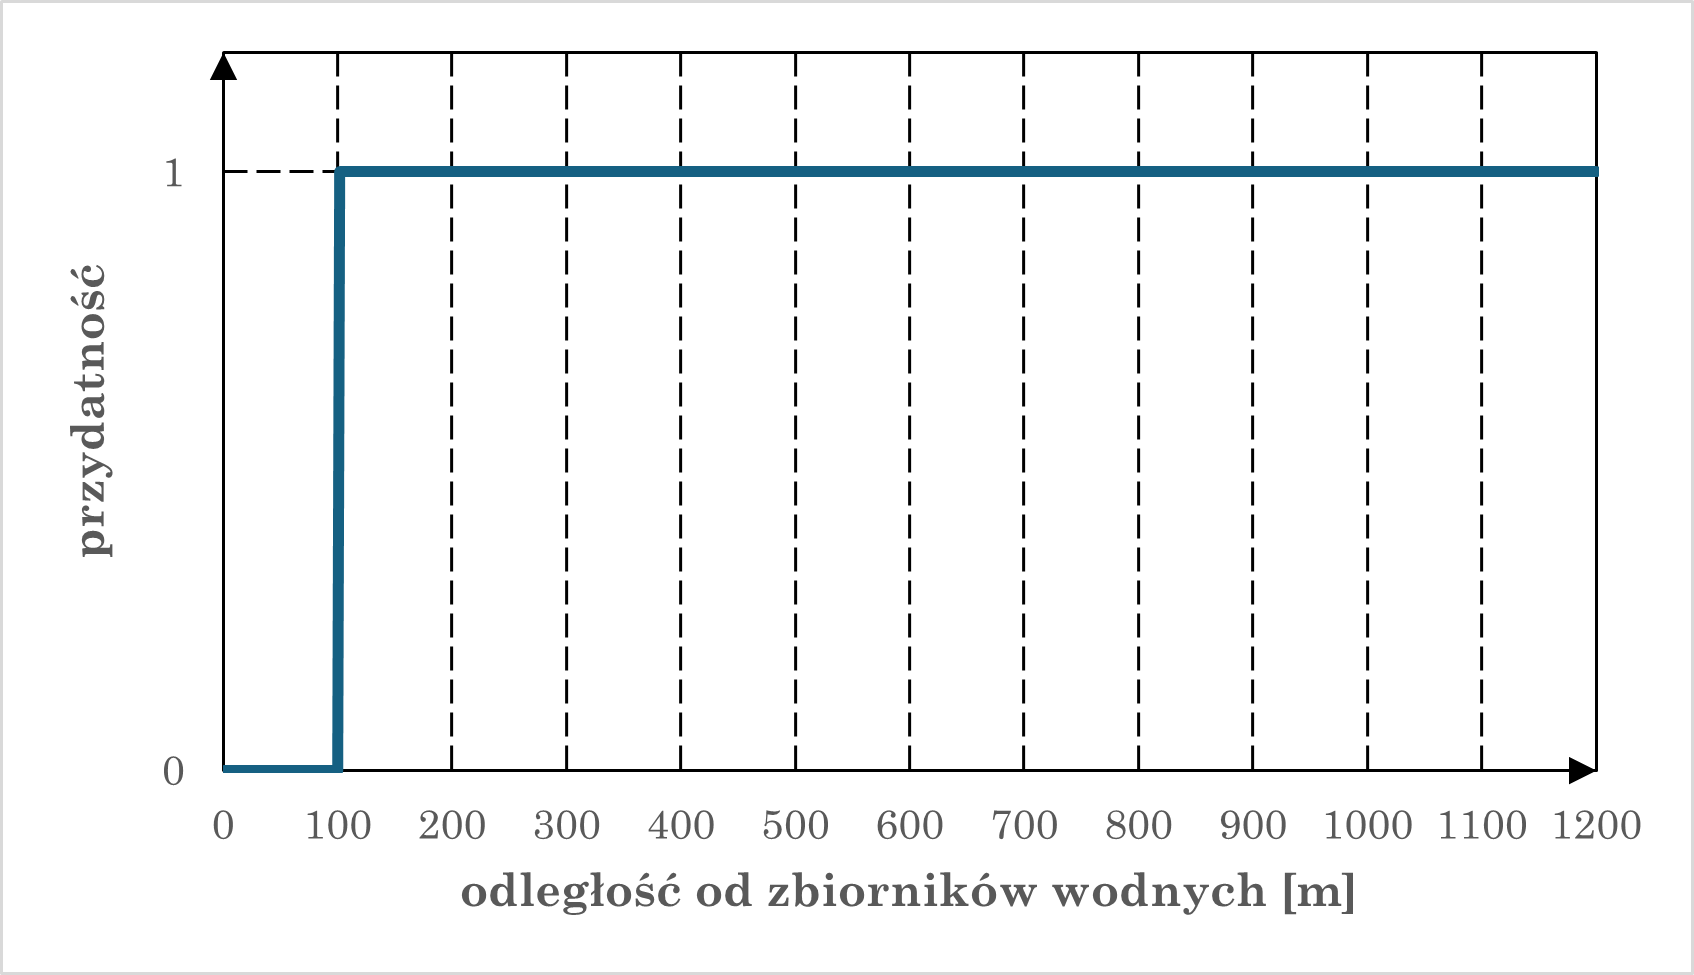
\includegraphics[width=\linewidth]{img/kryterium1-wykres-rosnaca.png}
        \caption{Funkcja rosnąca}
    \end{minipage}
    \begin{minipage}{0.48\textwidth}
        \centering
        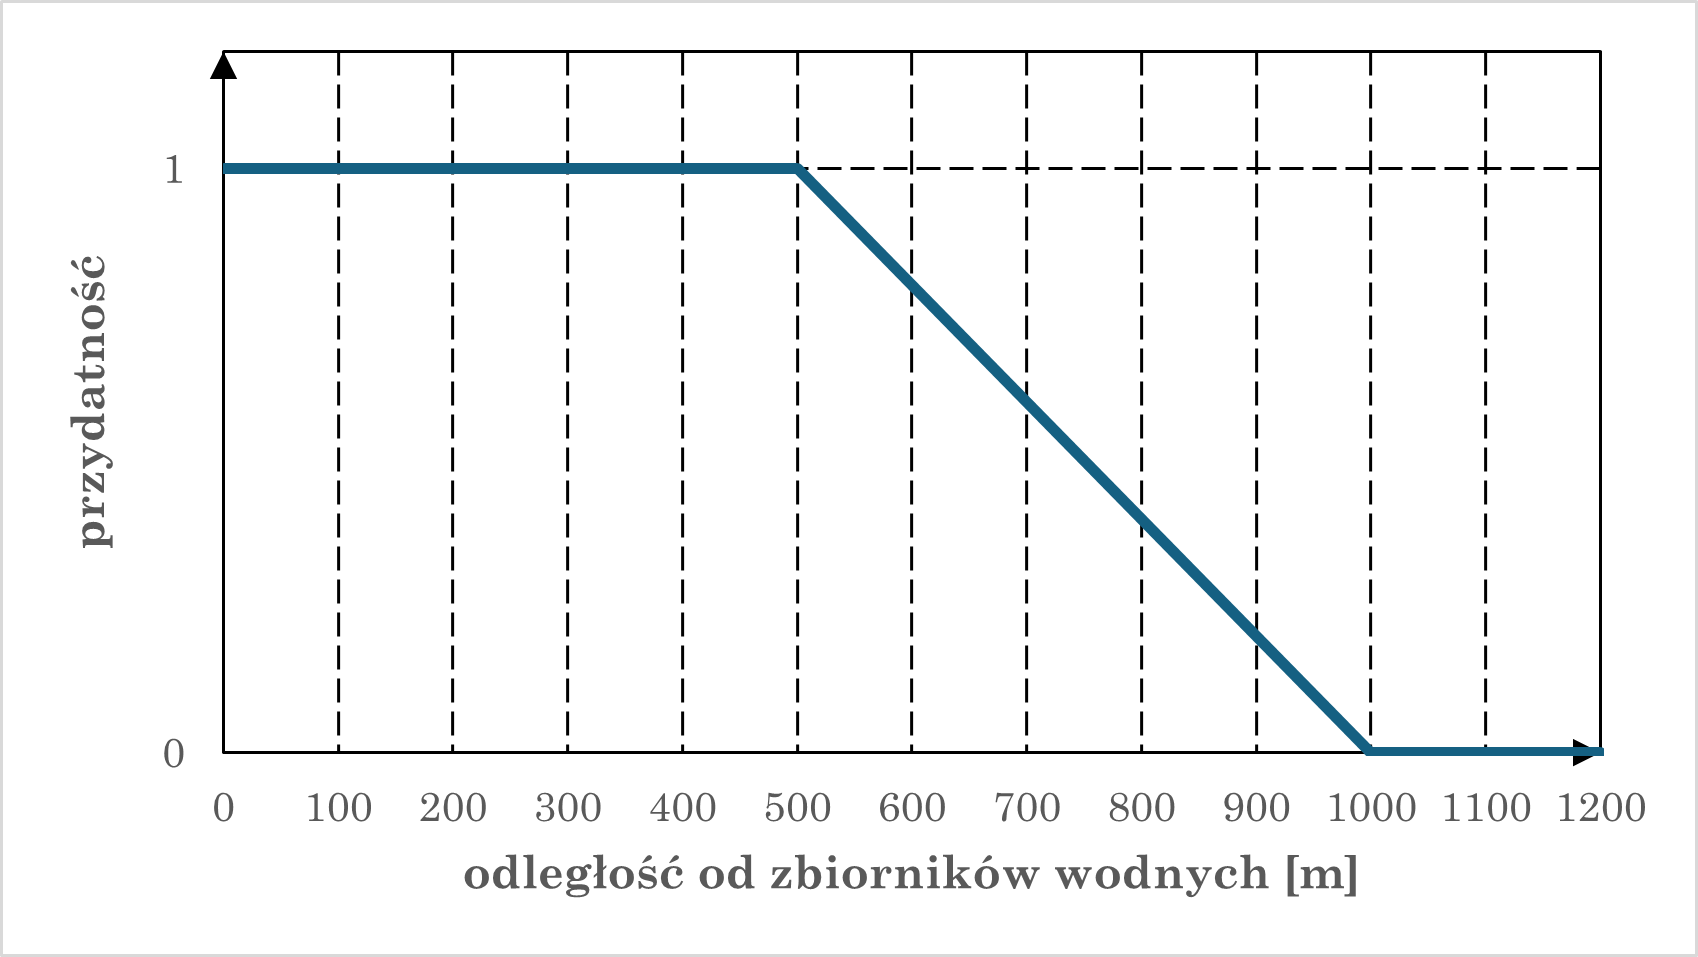
\includegraphics[width=\linewidth]{img/kryterium1-wykres-malejaca.png}
        \caption{Funkcja malejąca}
    \end{minipage}
\end{figure}
\vspace{10pt}

Ostateczny wynik kryterium pierwszego uzyskano po połączeniu obu warstw utworzonych wcześniej przy użyciu fuzzy logic. Wykorzystano do tego narzędzie \textit{FuzzyOverlay}.
\vspace{5pt}

\begin{mintedbox}{python}
woda_mapa = arcpy.sa.FuzzyOverlay([woda_rosnaca, woda_malejaca], 'AND')
woda_mapa.save(f'{geobaza}\\kryterium_1')
\end{mintedbox}
\vspace{5pt}

\begin{figure}[H]
    \centering
    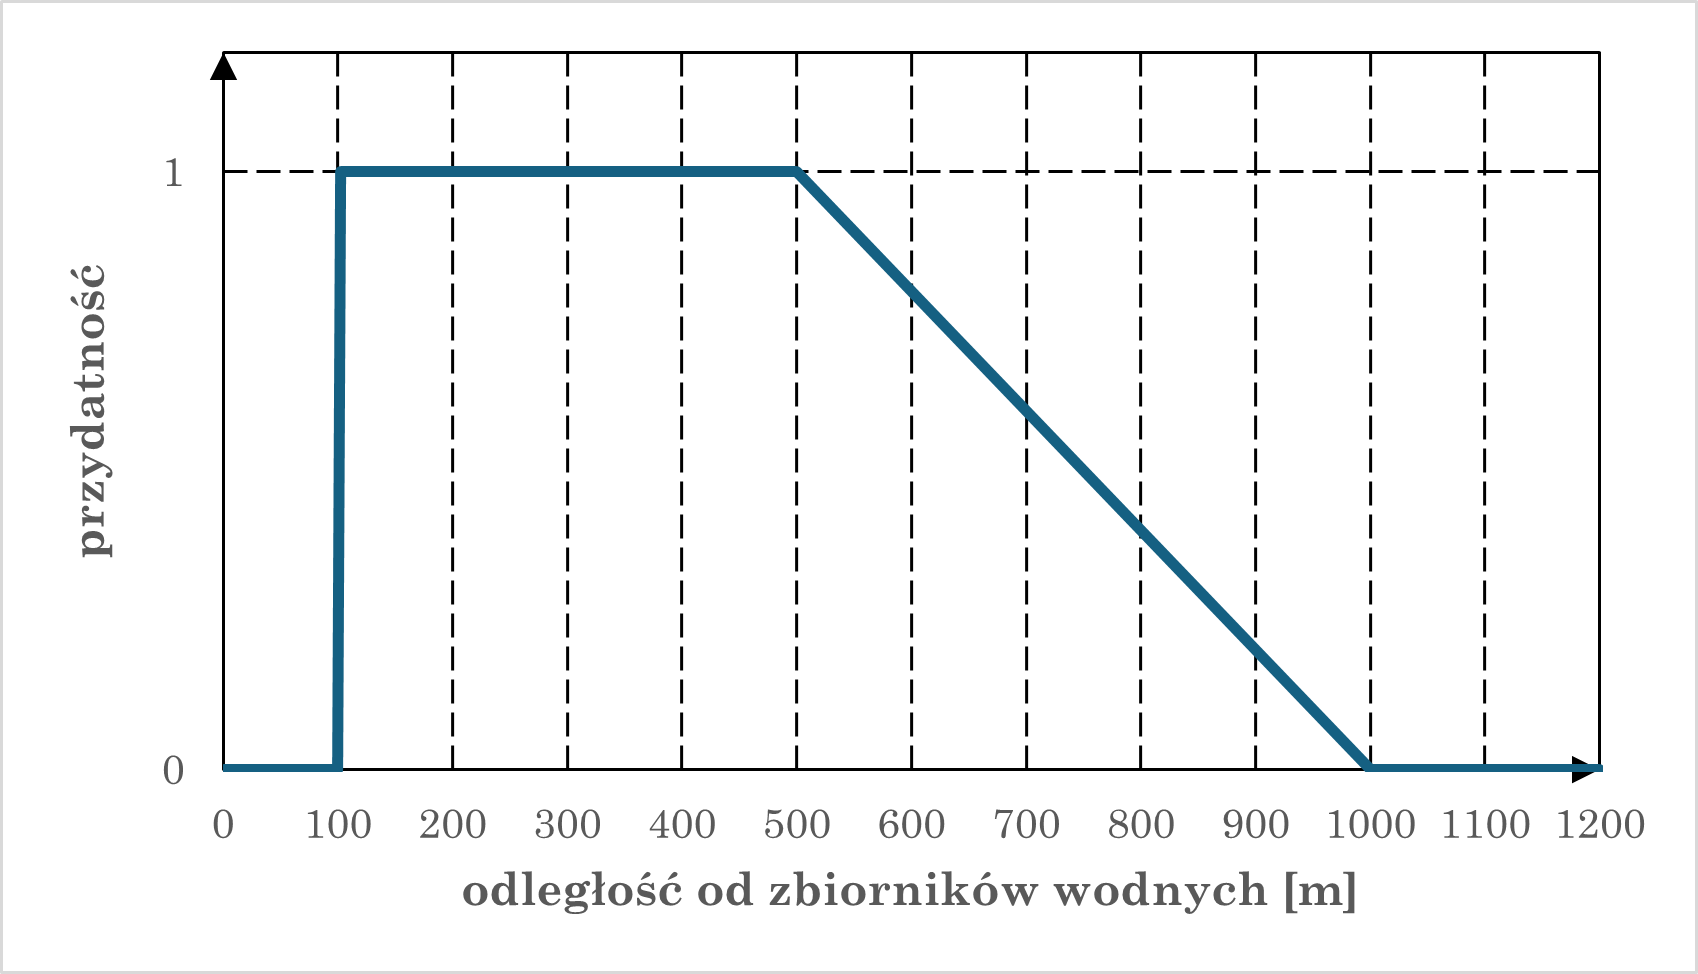
\includegraphics[width=0.6\textwidth]{img/kryterium1-wykres-glowny.png}
    \caption{Reklasyfikacja dla kryterium 1.}
\end{figure}
\newpage

Wynikiem analizy dla kryterium pierwszego była poniższa mapa. Wyklucza ona z przydatności wąską część obszaru położoną wokół wód. Reszta obszaru, ze względu na dosyć szeroki zakres odległości od wody, dla których przydatność reklasyfikowano na 1, ma korzystne warunki do inwestycji.
\vspace{5pt}

\begin{figure}[H]
    \centering
    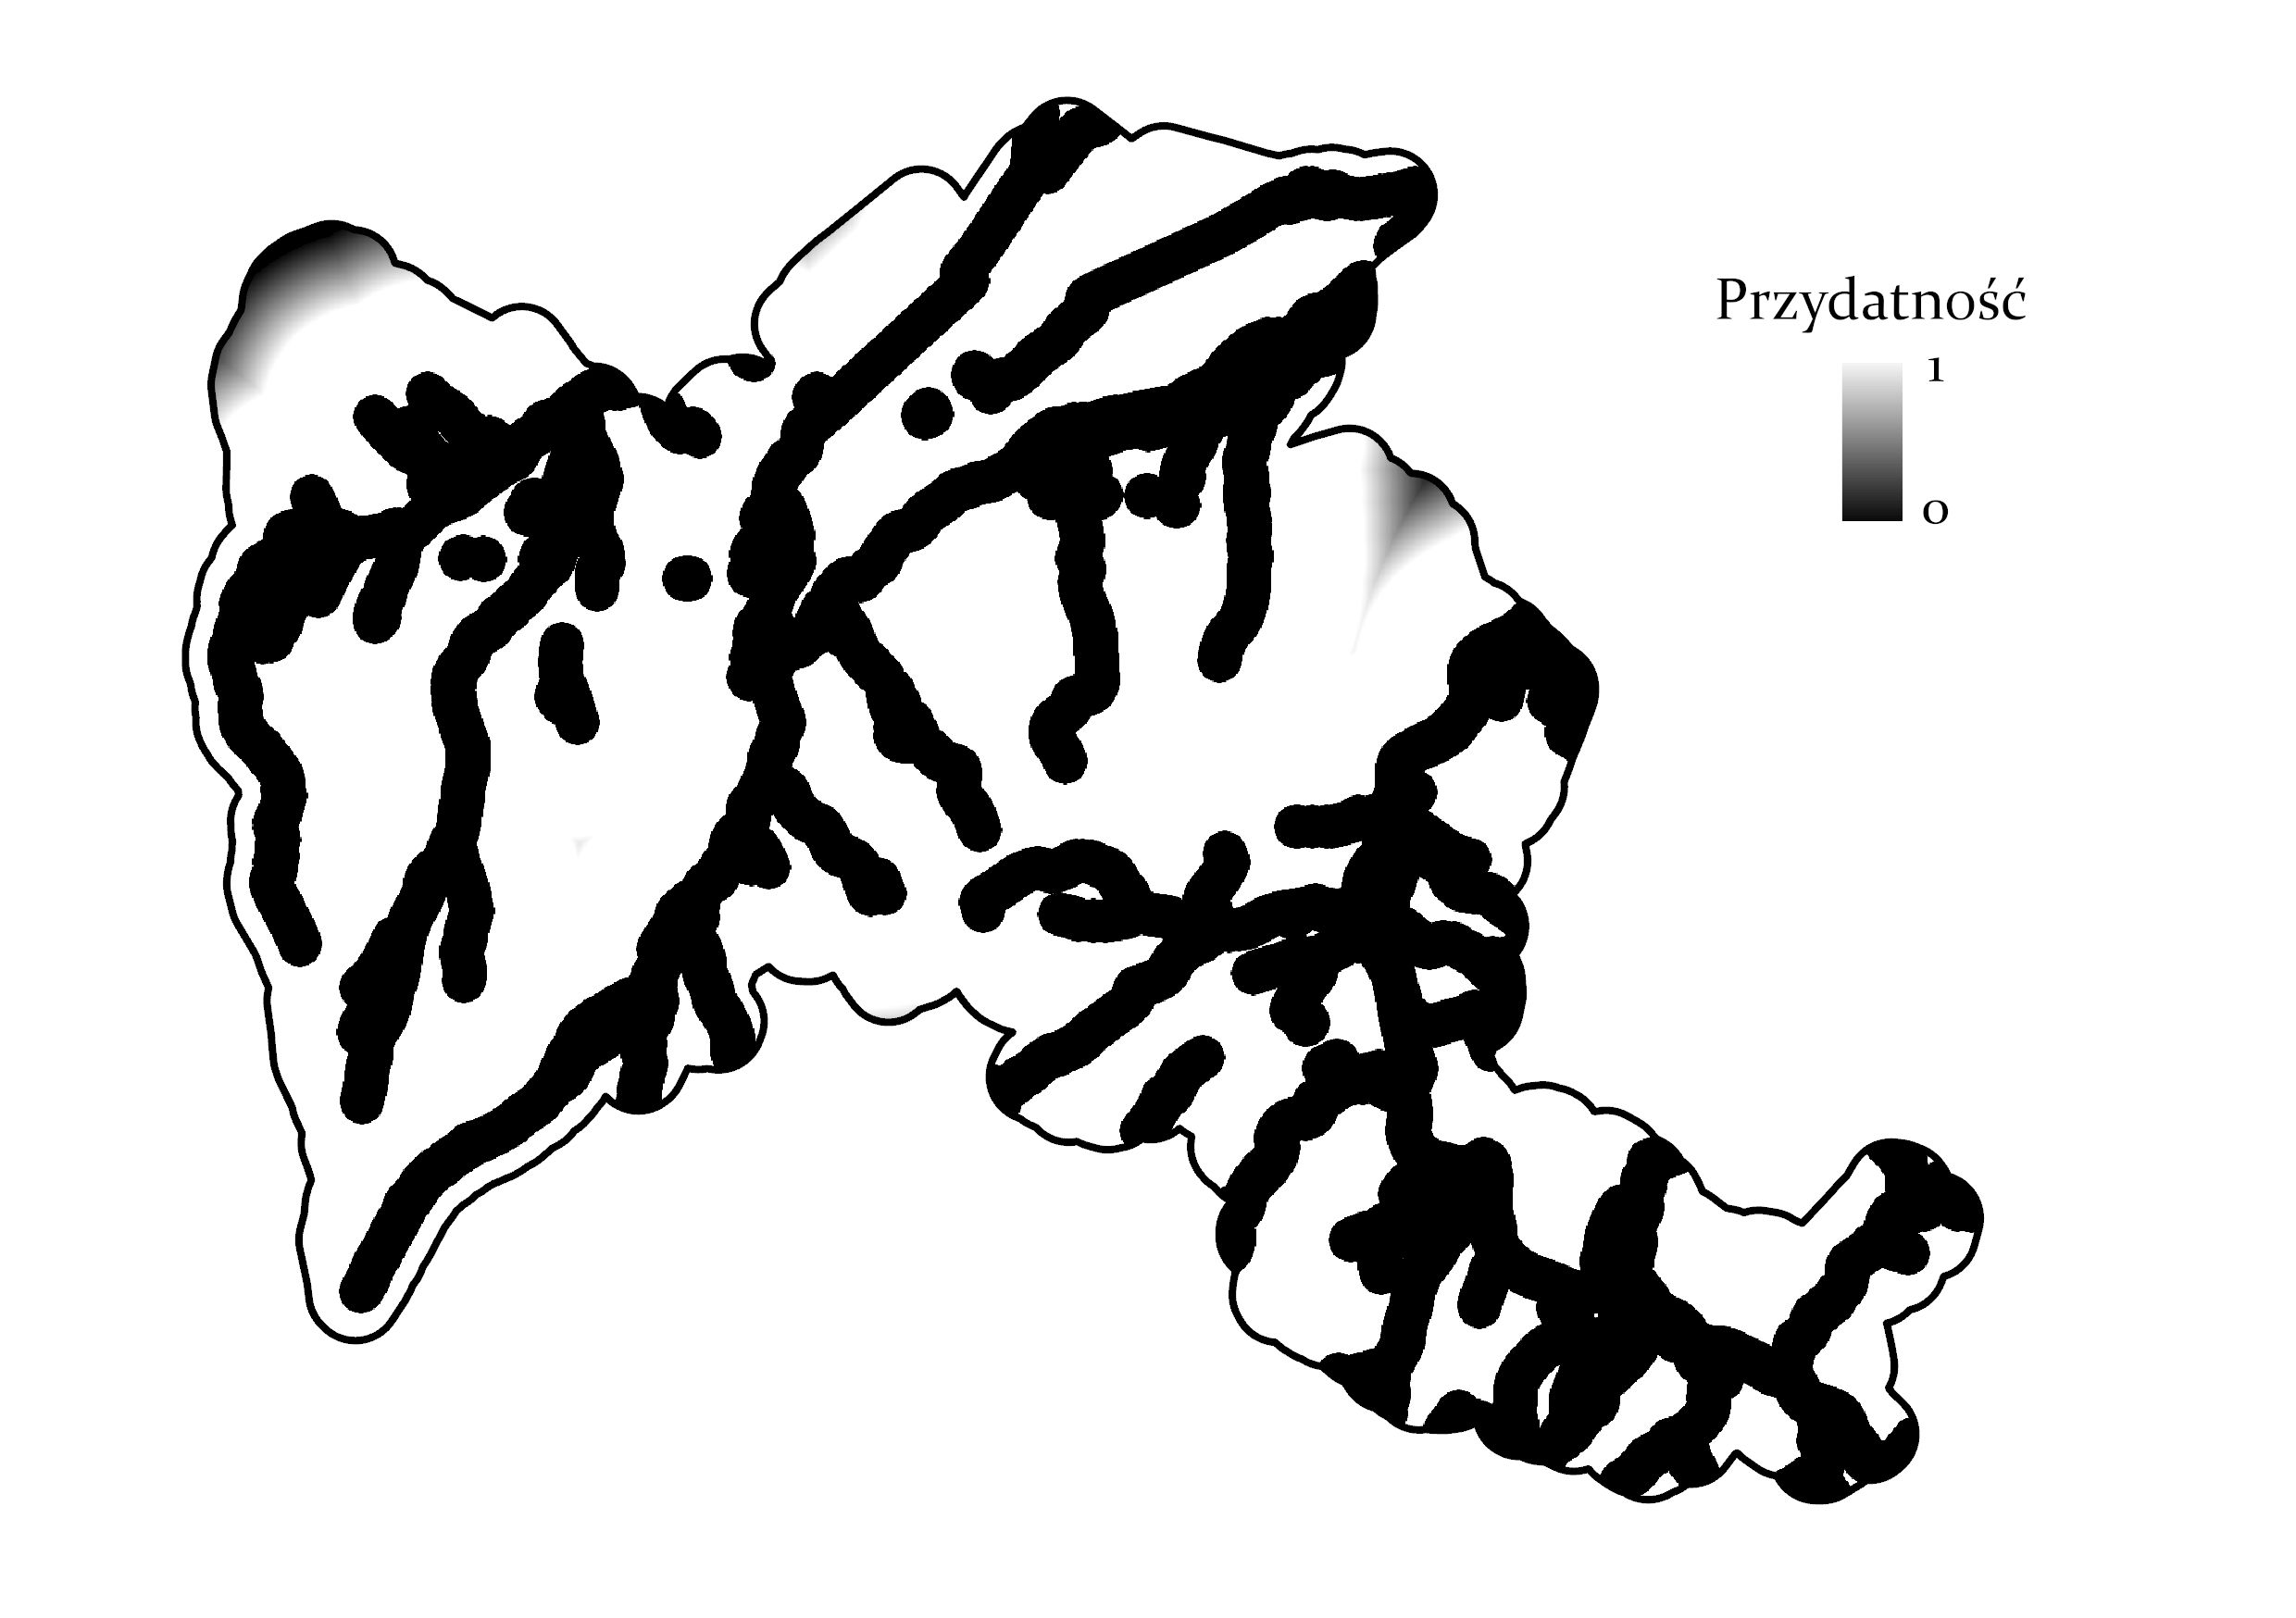
\includegraphics[width=0.75\textwidth]{img/kryterium1-layout.jpg}
    \caption{Mapa przydatności dla kryterium 1.}
\end{figure}
\vspace{10pt}

Mapę zapisano do geobazy w celu użycia w późniejszym etapie.
\vspace{5pt}

\begin{mintedbox}{python}
woda_mapa.save(f'{geobaza}\\kryterium_1')
\end{mintedbox}
\vspace{10pt}

Poniżej zaprezentowano mapę przedstawiającą rzeki i wody powierzchniowe na tle utworzonej mapy przydatności.

\begin{figure}[H]
    \centering
    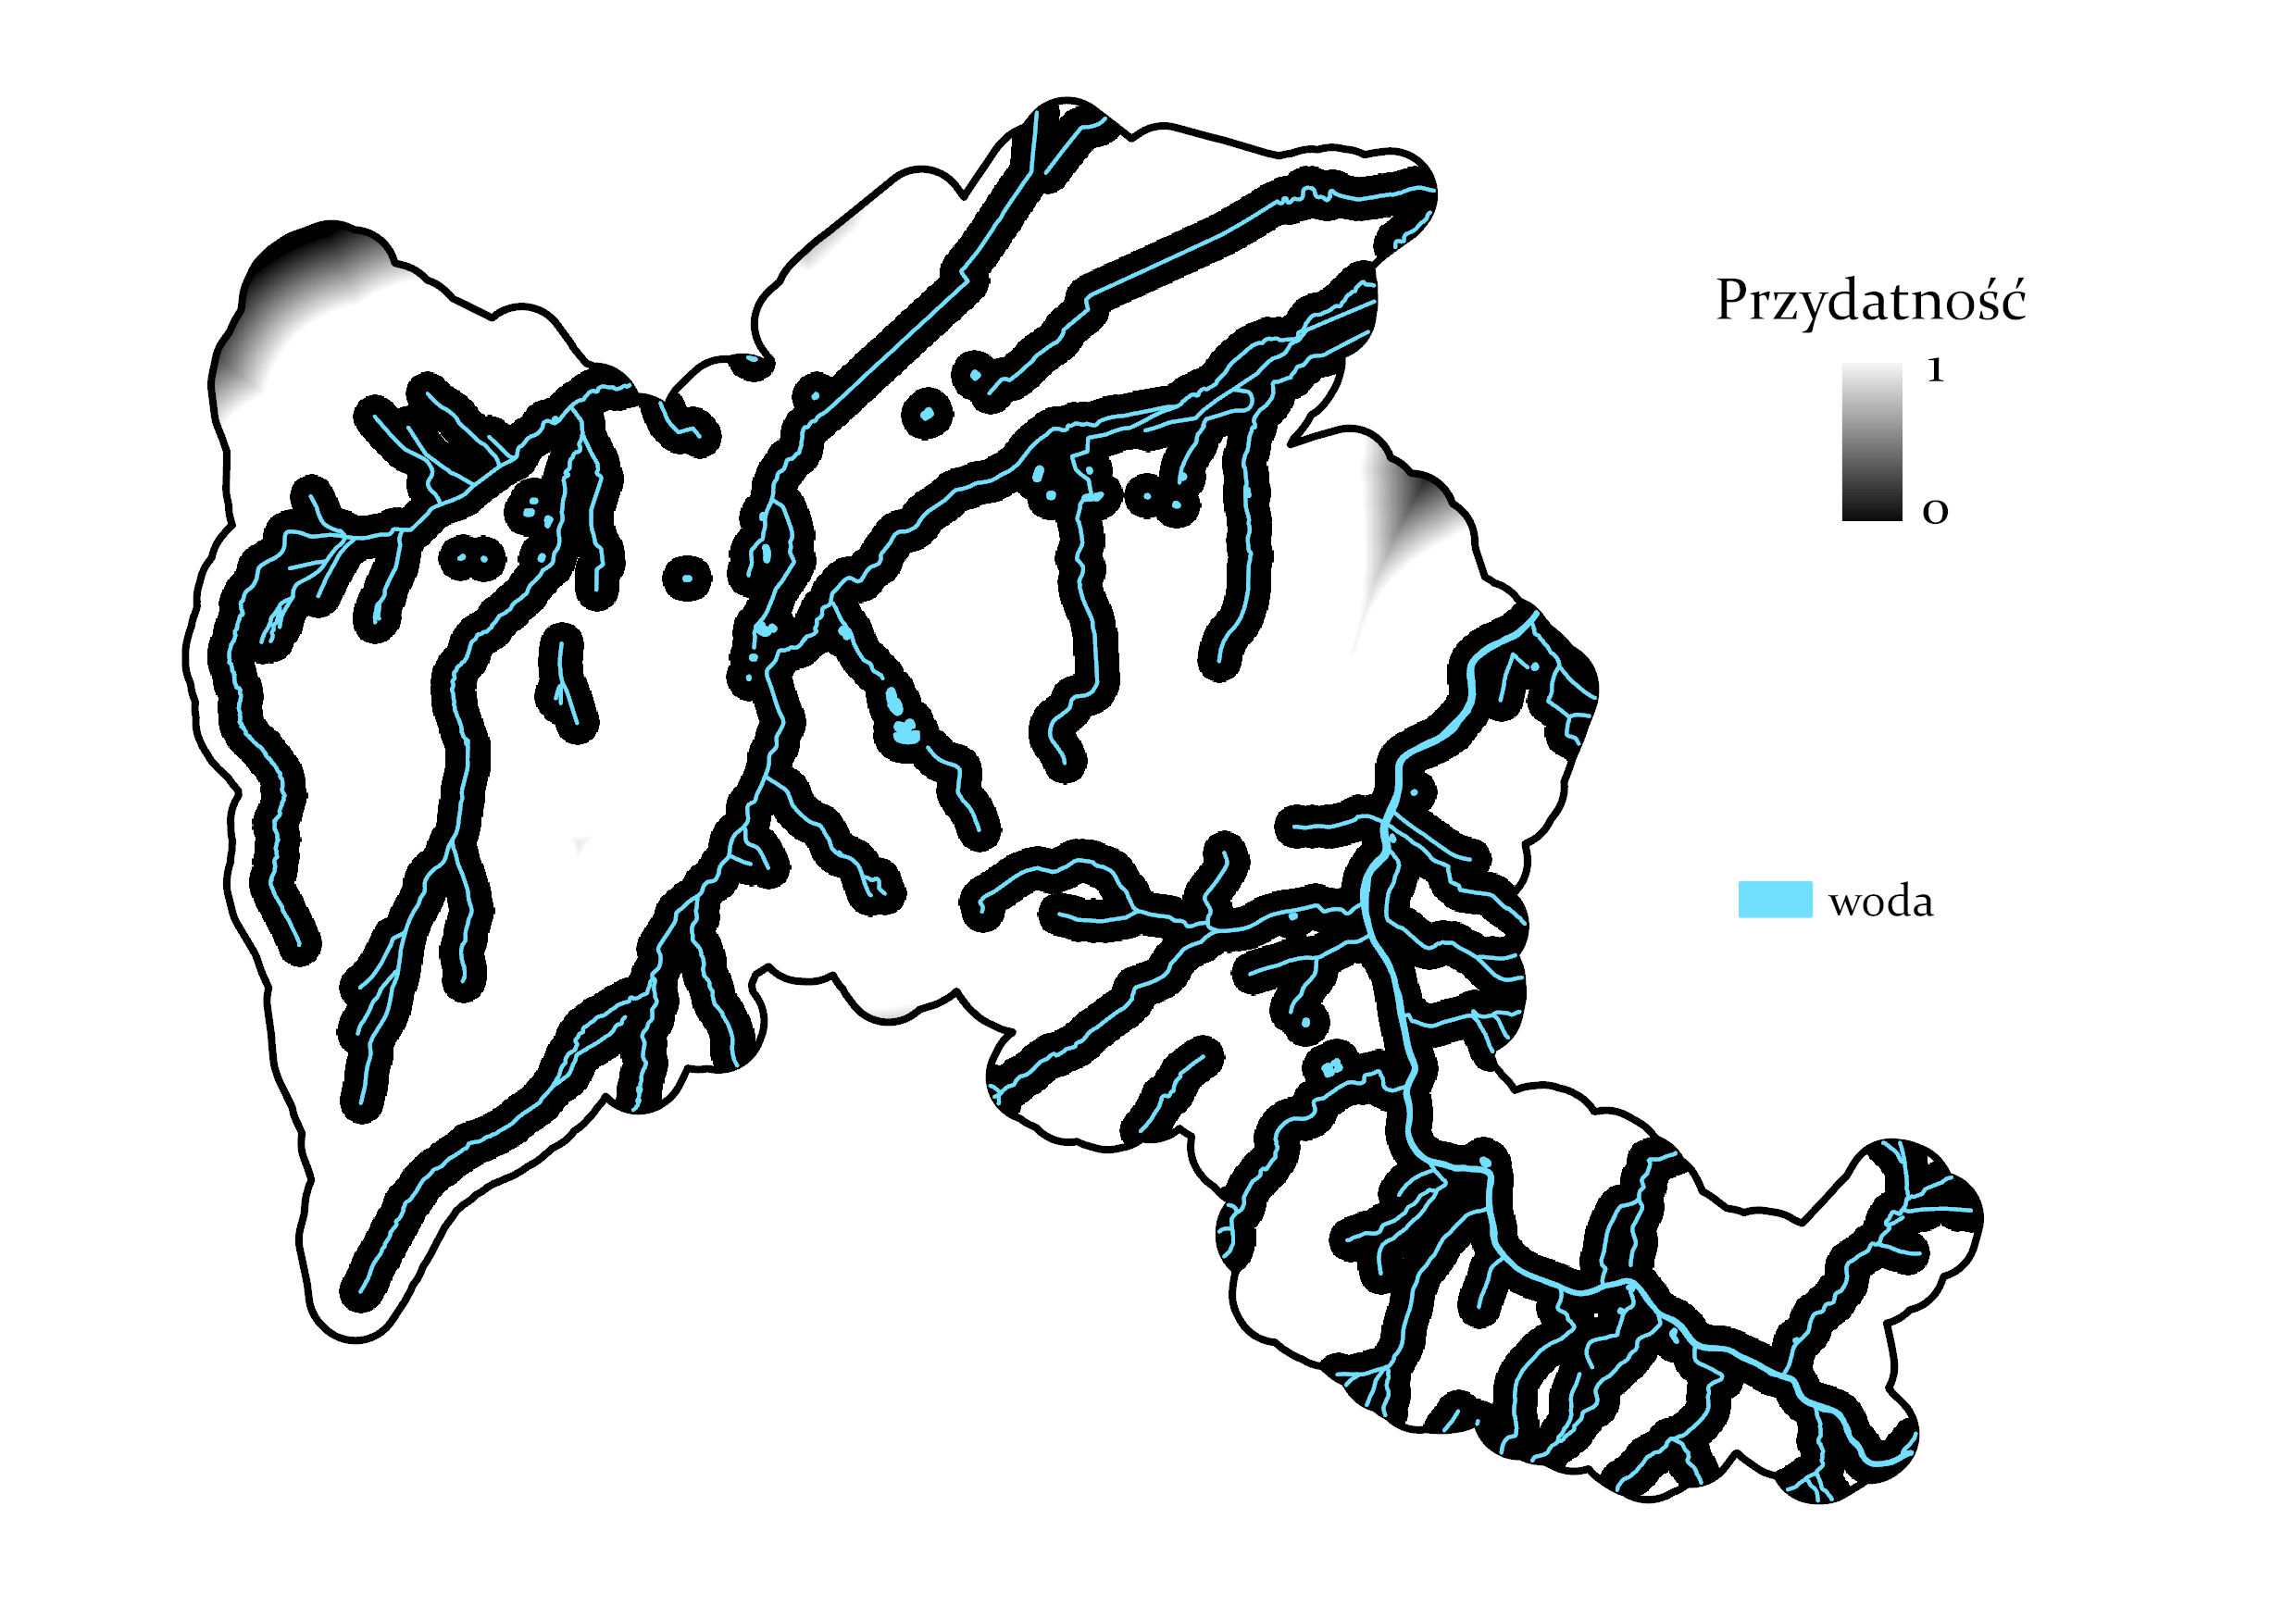
\includegraphics[width=0.75\textwidth]{img/kryterium1-woda.jpg}
    \caption{Mapa przydatności dla kryterium 1. zawierająca rzeki oraz zbiorniki wodne}
\end{figure}
\vspace{10pt}

\subsection{Kryterium 2: odległość od budynków mieszkalnych}
W celu rozpatrzenia kryterium odległościowego od budynków mieszkalnych, pobrano z bazy BDOT10k poligonową warstwę o kodzie OT\_BUBD\_A, reprezentującą budynki. Następnie wybrano z nich jedynie te będące budynkami mieszkalnymi. Skorzystano w tym celu z atrybutu \textit{FOBUD} warstwy, informującego o funkcji ogólnej budynku. Budynki mieszkalne przyjmowały w tym polu wartość \textit{budynki mieszkalne}. Skonstruowano więc zapytanie i wybrano zgodne obiekty, korzystając z funkcji \textit{Select} z zestawu {Analysis}.
\vspace{5pt}

\begin{mintedbox}{python}
arcpy.analysis.Select(budynki, 'budynki_mieszkalne', "FOBUD = 'budynki mieszkalne'")
\end{mintedbox}
\vspace{10pt}

Następnie utworzono raster reprezentujący odległość od budynku mieszkalnego dla każdej komórki z użyciem narzędzia \textit{DistanceAccumulation}.
\vspace{5pt}

\begin{mintedbox}{python}
out_distance_accumulation_buildings = arcpy.sa.DistanceAccumulation(in_source_data='budynki_mieszkalne')
\end{mintedbox}
\vspace{10pt}

Dla utworzonej warstwy dokonano określenia członkostwa z użyciem rosnącej funkcji liniowej. Funkcja każdej komórce odległej od budynku mieszkalnego o mniej niż 150 metrów przyporządkowywała zerową przydatność. Dla obszarów odległych od 150 do 300 metrów przydatność liniowo rosła, i od 300 metrów w górę przyjmowała maksymalną przydatność.
\vspace{5pt}

\begin{mintedbox}{python}
budynki_mieszkalne = arcpy.sa.FuzzyMembership(out_distance_accumulation_buildings, fuzzy_function="LINEAR 150 300")
\end{mintedbox}
\vspace{10pt}

Reklasyfikacji dokonano zgodnie z funkcją przedstawioną poniżej.
\vspace{5pt}

\begin{figure}[H]
    \centering
    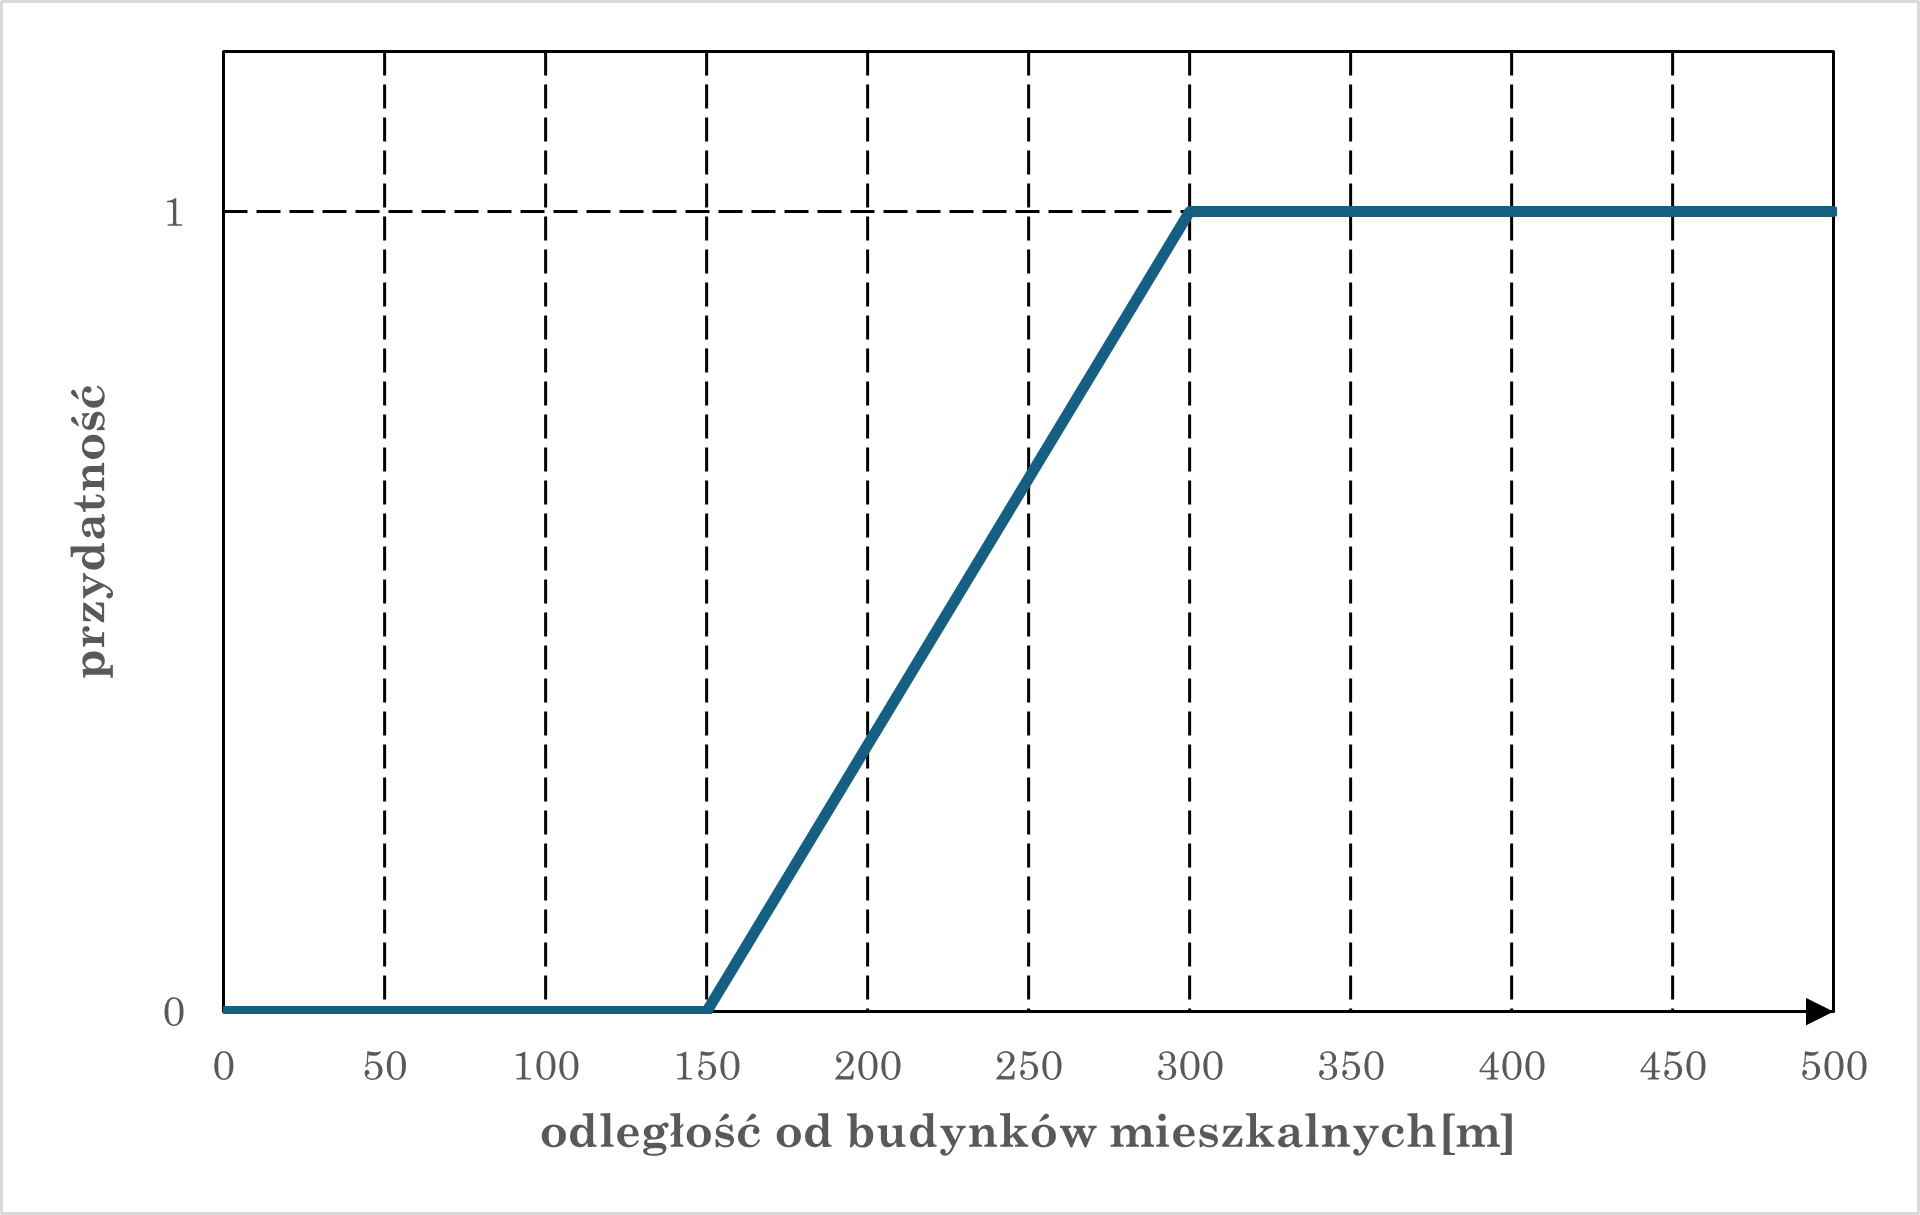
\includegraphics[width=0.6\textwidth]{img/kryterium2-wykres-glowny.png}
    \caption*{Reklasyfikacja dla kryterium 2.}
\end{figure}

\newpage

Wynikiem analizy dla kryterium drugiego była poniższa mapa. Wyklucza ona z przydatności znaczną część obszaru położoną w południowej oraz środkowo-zachodniej części gminy. Północna, zachodnia oraz centralna część obszaru przyjmuje maksymalną przydatność.
\vspace{5pt}

\begin{figure}[H]
    \centering
    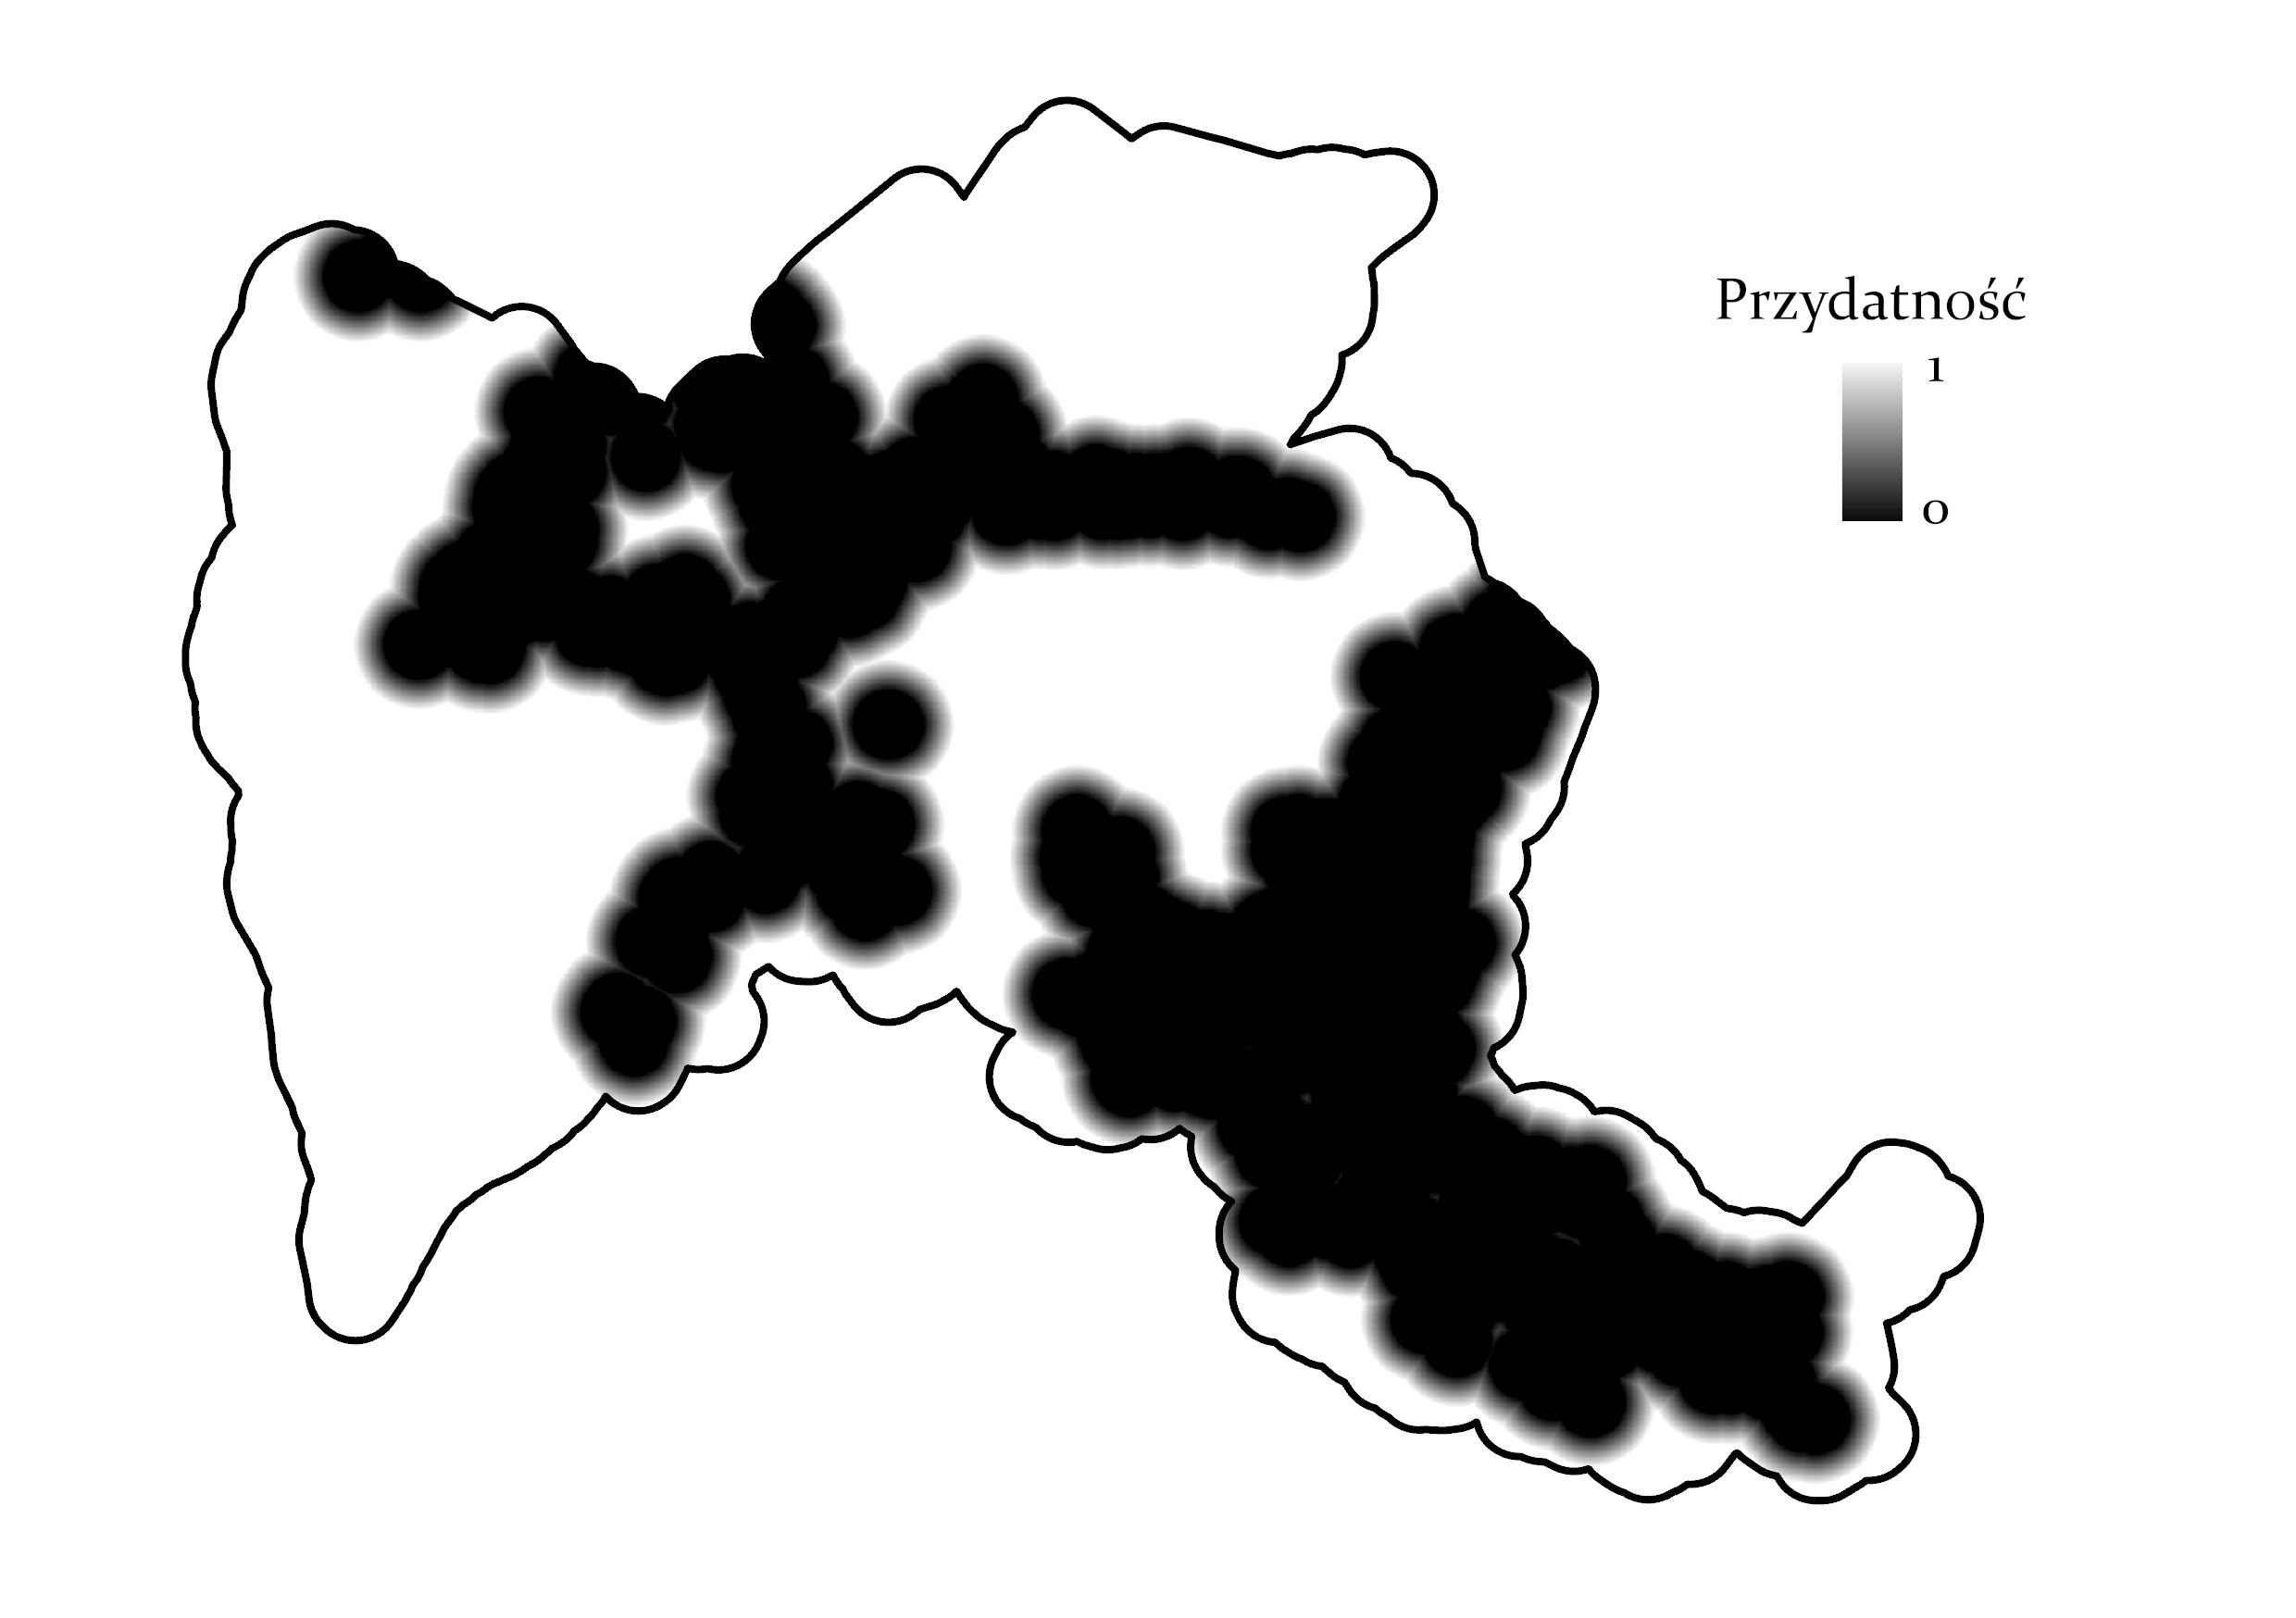
\includegraphics[width=0.75\textwidth]{img/kryterium2-layout.jpg}
    \caption{Mapa przydatności dla kryterium 2.}
\end{figure}
\vspace{10pt}

Mapę zapisano do geobazy w celu użycia w późniejszym etapie.
\vspace{5pt}

\begin{mintedbox}{python}
budynki_mieszkalne.save(f'{geobaza}\\kryterium_2')
\end{mintedbox}
\vspace{10pt}

Poniżej zaprezentowano mapę przedstawiającą budynki mieszkalne na tle utworzonej mapy przydatności.

\begin{figure}[H]
    \centering
    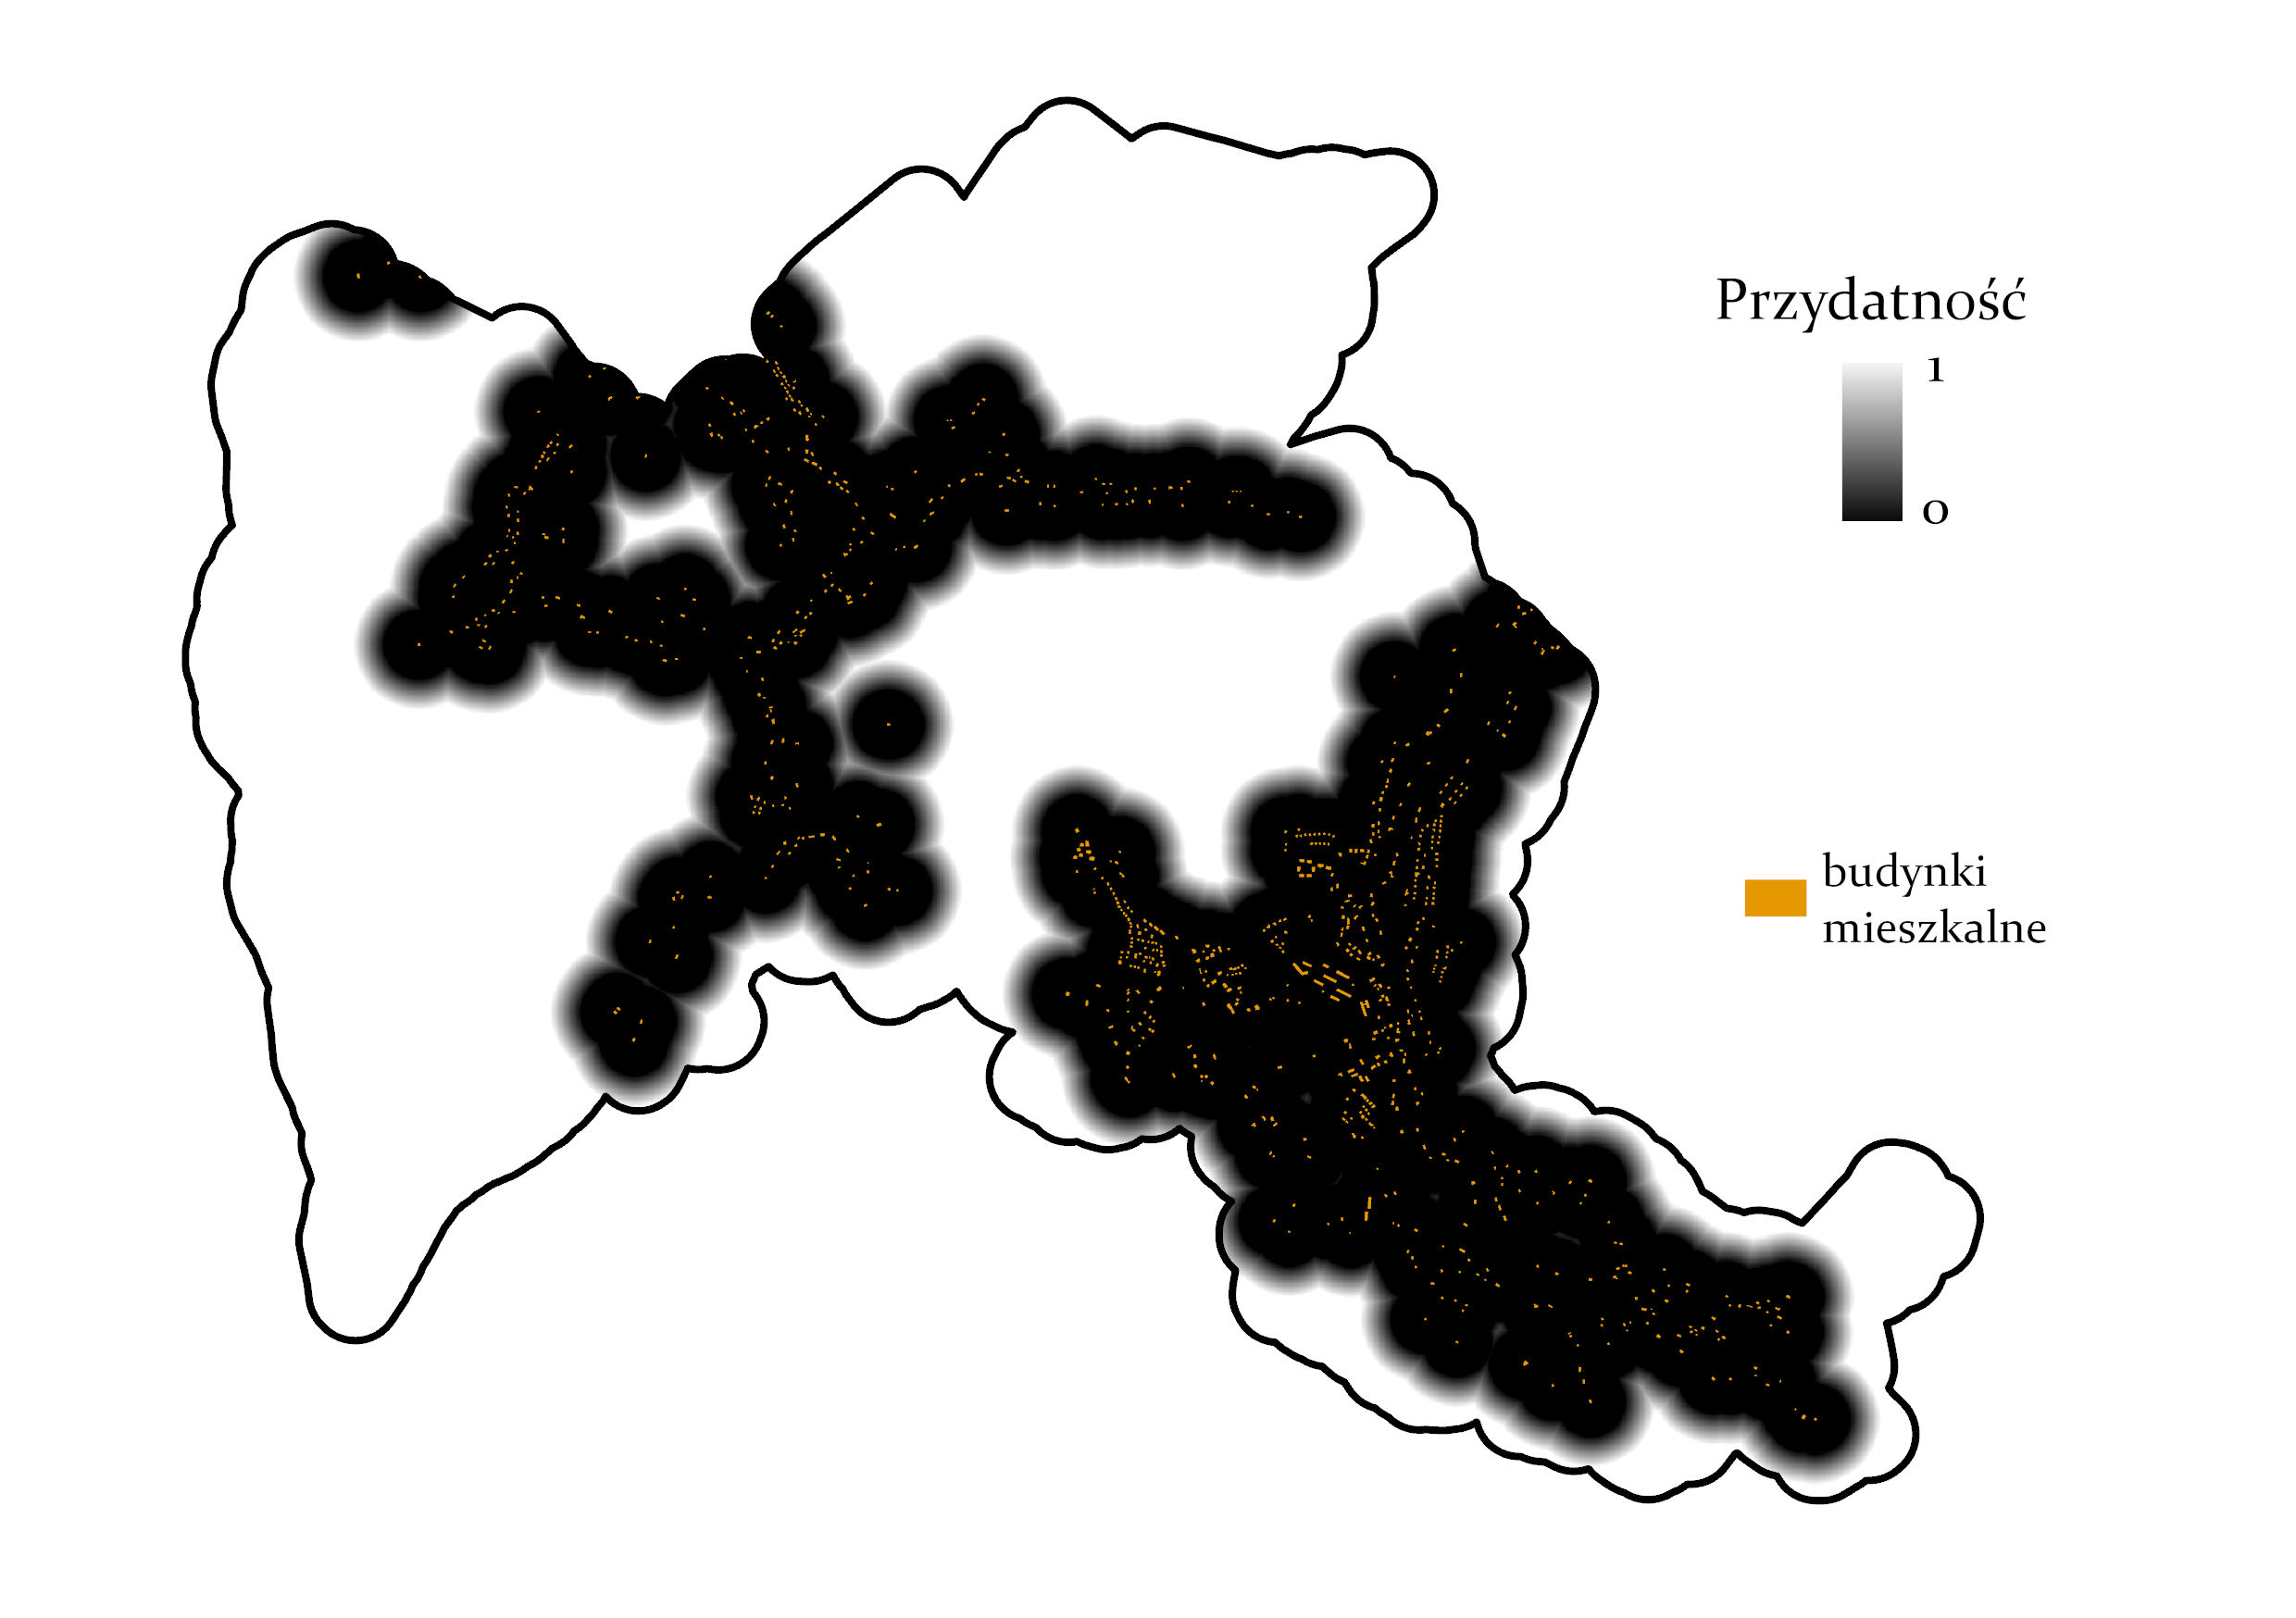
\includegraphics[width=0.75\textwidth]{img/kryterium2-budynki.jpg}
    \caption{Mapa przydatności dla kryterium 2. zawierająca budynki mieszkalne}
\end{figure}
\vspace{10pt}

\subsection{Kryterium 3: pokrycie terenu}
Warstwą wejściową w kryterium trzecim, była warstwa OT\_PTLZ\_A zawierająca tereny leśne i zadrzewione. W celu obliczenia odległości komórek od terenów leśnych, wykorzystano funkcję \textit{DistanceAccumulation}.
\vspace{5pt}

\begin{mintedbox}{python}
out_distance_accumulation_ptlz = arcpy.sa.DistanceAccumulation(in_source_data=ptlz)
\end{mintedbox}
\vspace{10pt}

Następnie określono poziom członkostwa z użyciem FuzzyMembership. Funkcja każdej komórce odległej od lasu o mniej niż 15 metrów przyporządkowywała zerową przydatność. Dla obszarów odległych od 15 do 100 metrów przydatność liniowo rosła, przyjmując od 100 metrów w górę maksymalną przydatność.
\vspace{5pt}

\begin{mintedbox}{python}
lasy_fuzzy = arcpy.sa.FuzzyMembership(out_distance_accumulation_ptlz, fuzzy_function="LINEAR 15 100")
\end{mintedbox}
\vspace{10pt}

Reklasyfikacji dokonano zgodnie z funkcją przedstawioną poniżej.
\vspace{5pt}

\begin{figure}[H]
    \centering
    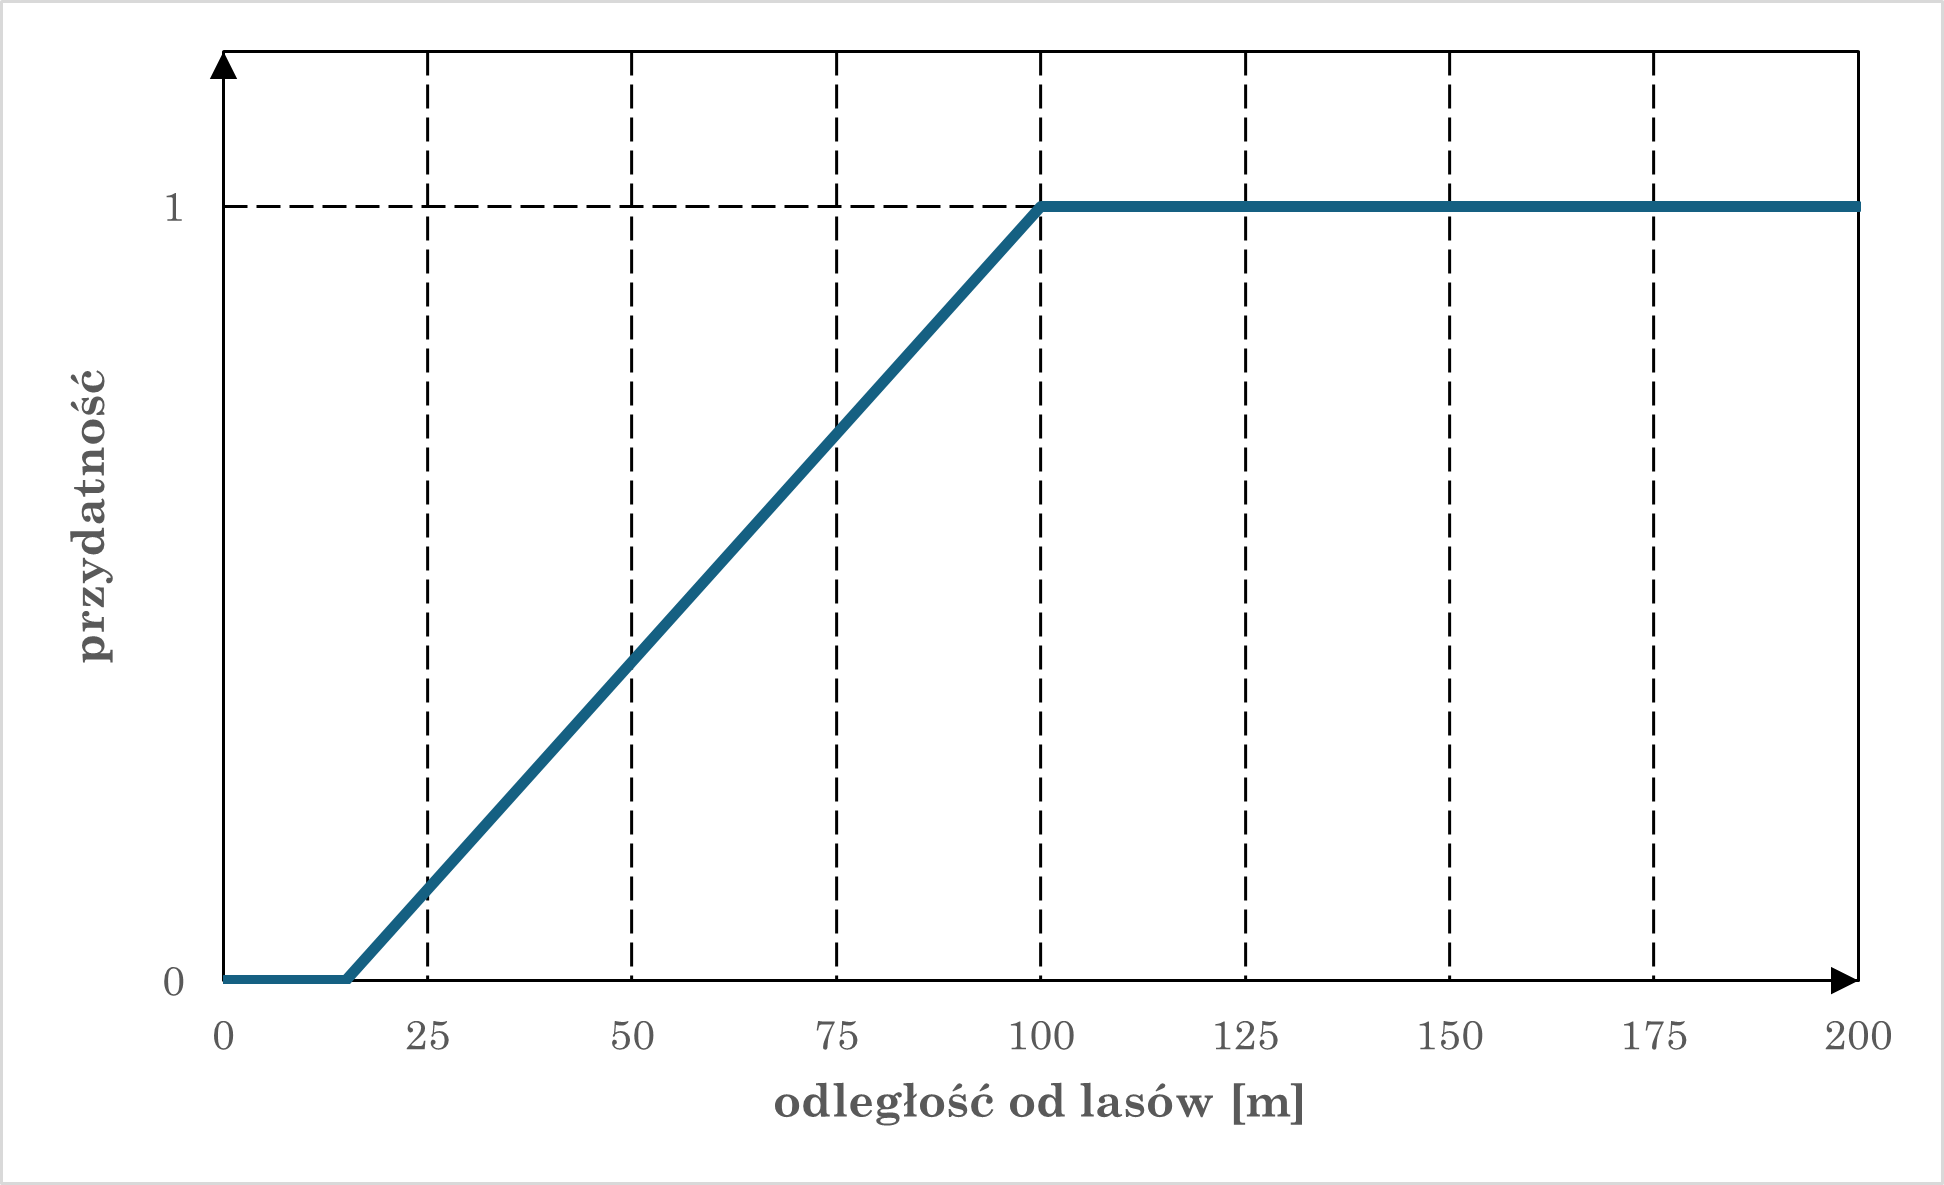
\includegraphics[width=0.6\textwidth]{img/kryterium3-wykres-glowny.png}
    \caption*{Reklasyfikacja dla kryterium 3.}
\end{figure}
\vspace{10pt}

Wynikiem analizy dla kryterium drugiego była poniższa mapa. Ze względu na wysoką lesistość lub niewielką odległość od lasu większość obszaru gminy została wyeliminowana. Przydatny pozostał obszar w północnej części gminy oraz częściowo w południowo-wschodniej.
\vspace{5pt}

\begin{figure}[H]
    \centering
    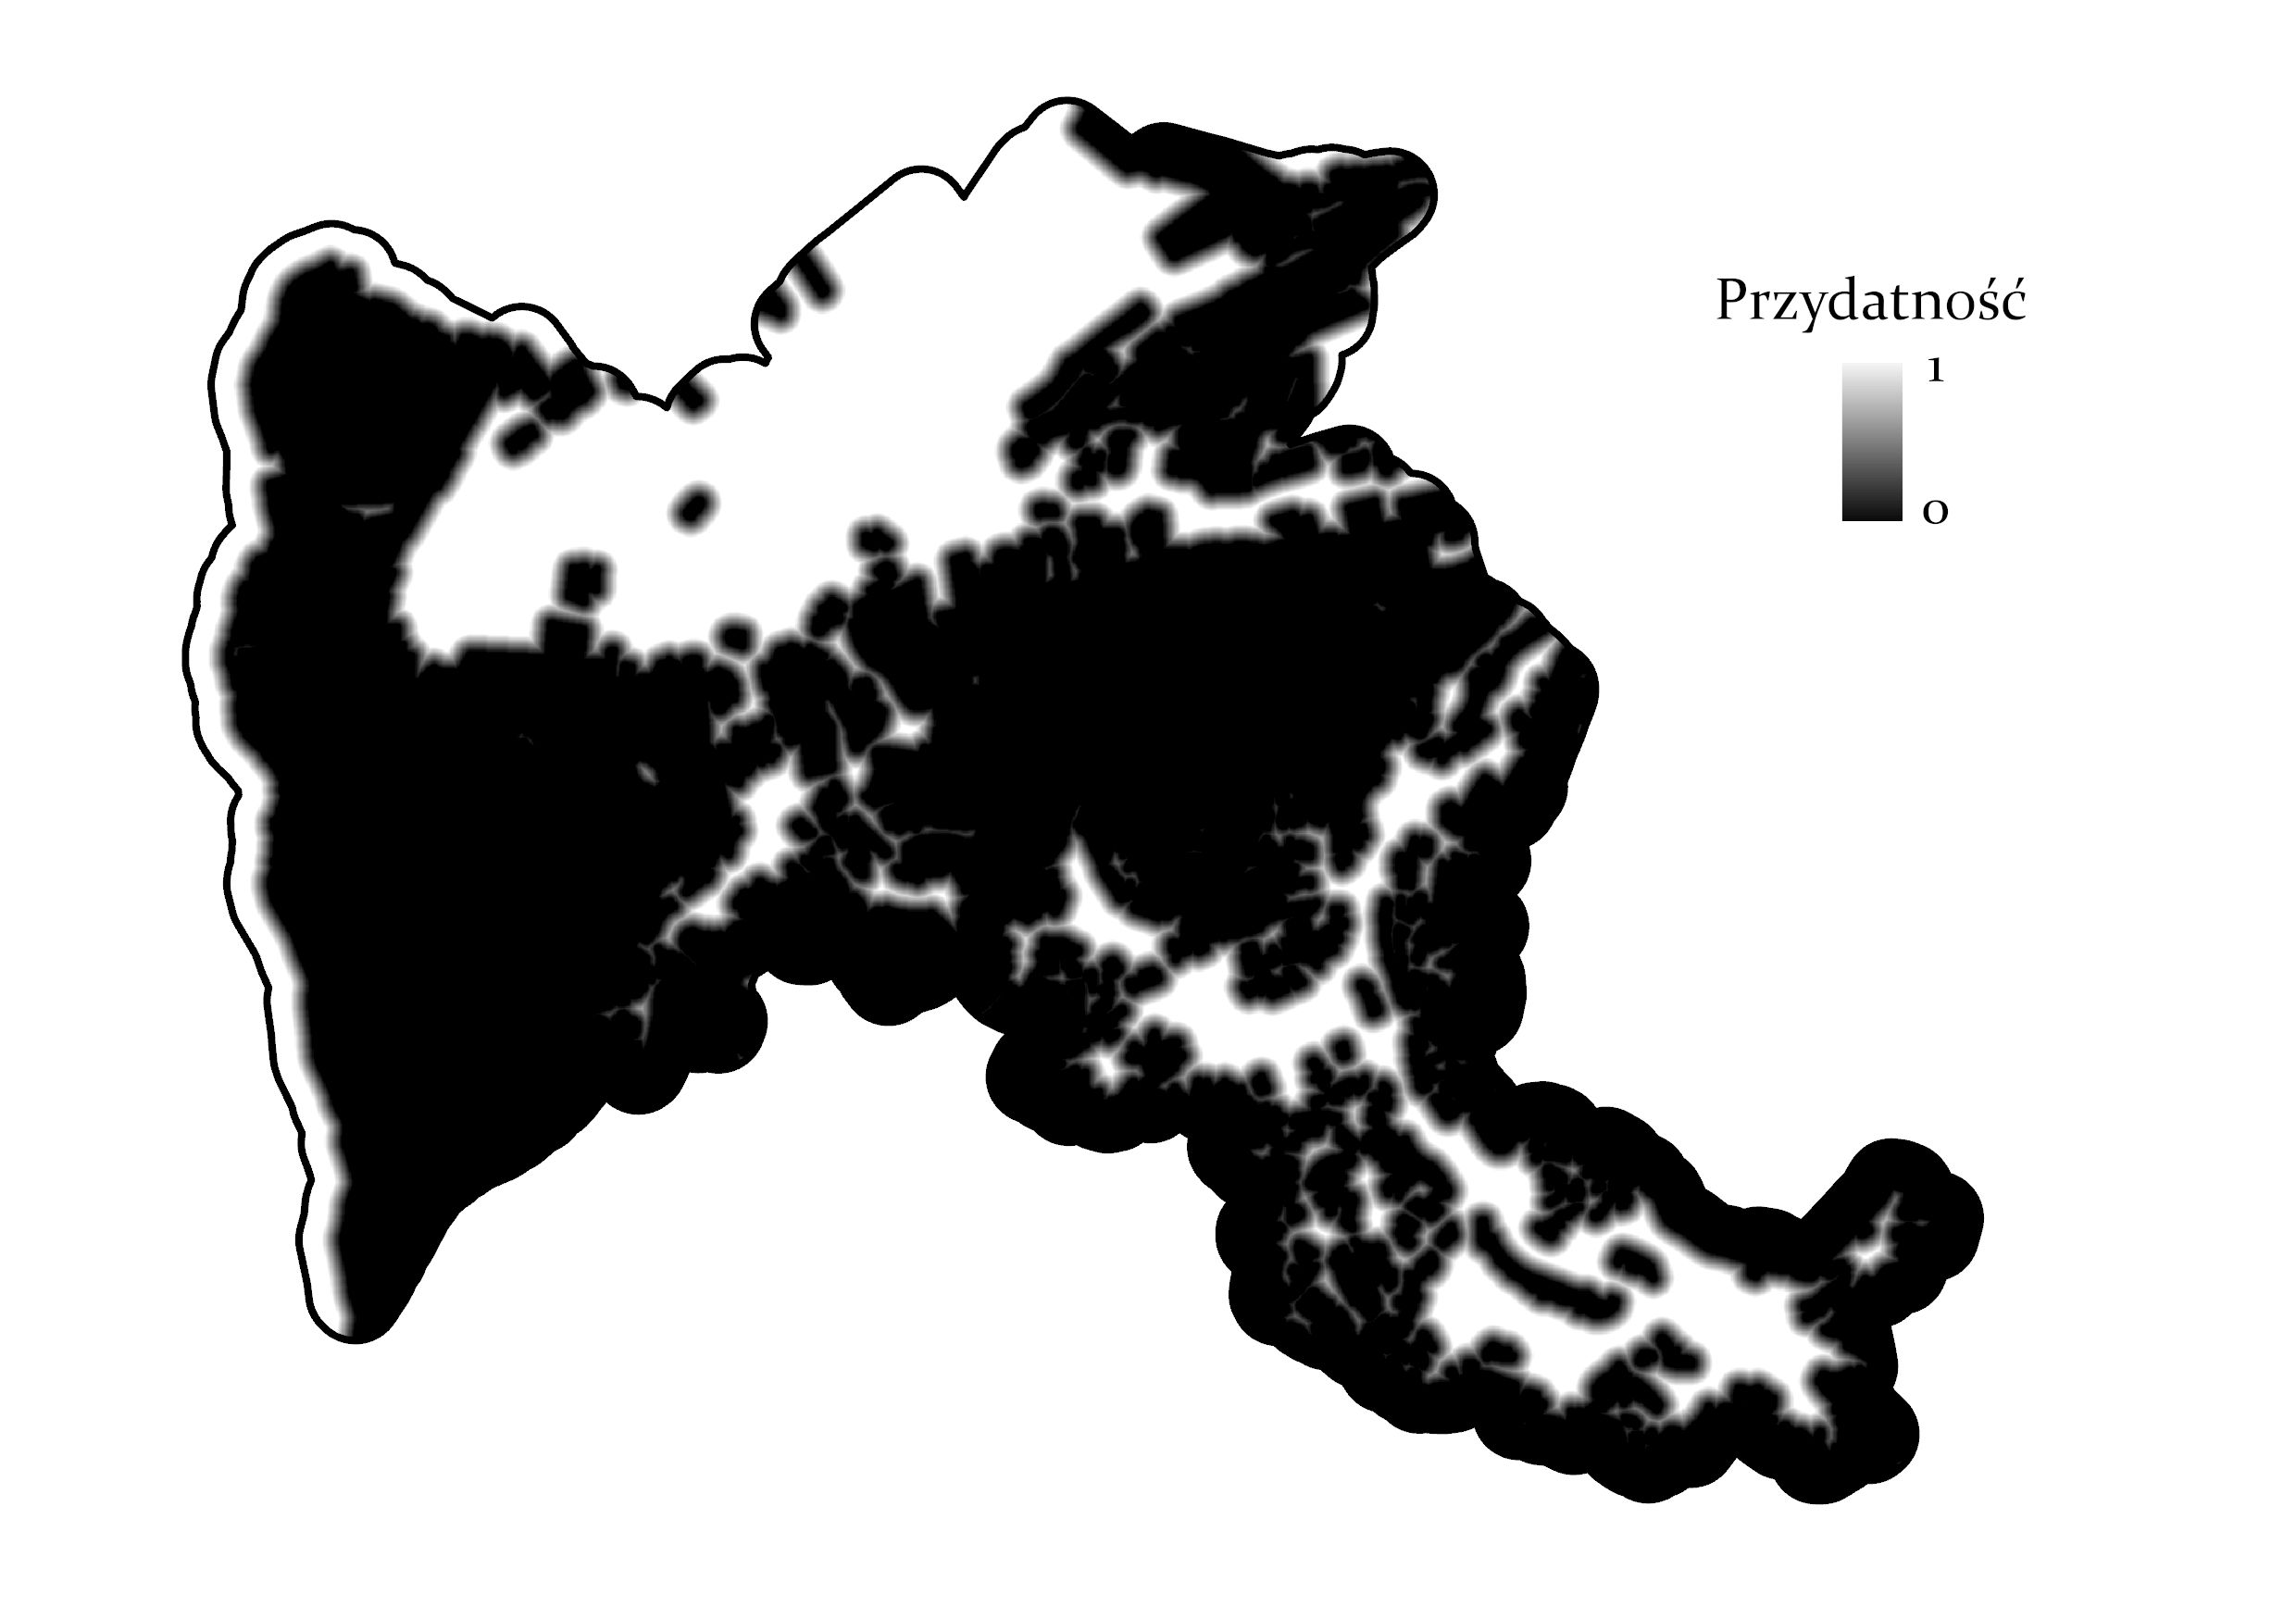
\includegraphics[width=0.75\textwidth]{img/kryterium3-layout.jpg}
    \caption{Mapa przydatności dla kryterium 3.}
\end{figure}
\vspace{10pt}

Mapę zapisano do geobazy w celu użycia w późniejszym etapie.
\vspace{5pt}

\begin{mintedbox}{python}
budynki_mieszkalne.save(f'{geobaza}\\kryterium_3')
\end{mintedbox}
\vspace{10pt}

Poniżej zaprezentowano mapę przedstawiającą lasy na tle utworzonej mapy przydatności.

\begin{figure}[H]
    \centering
    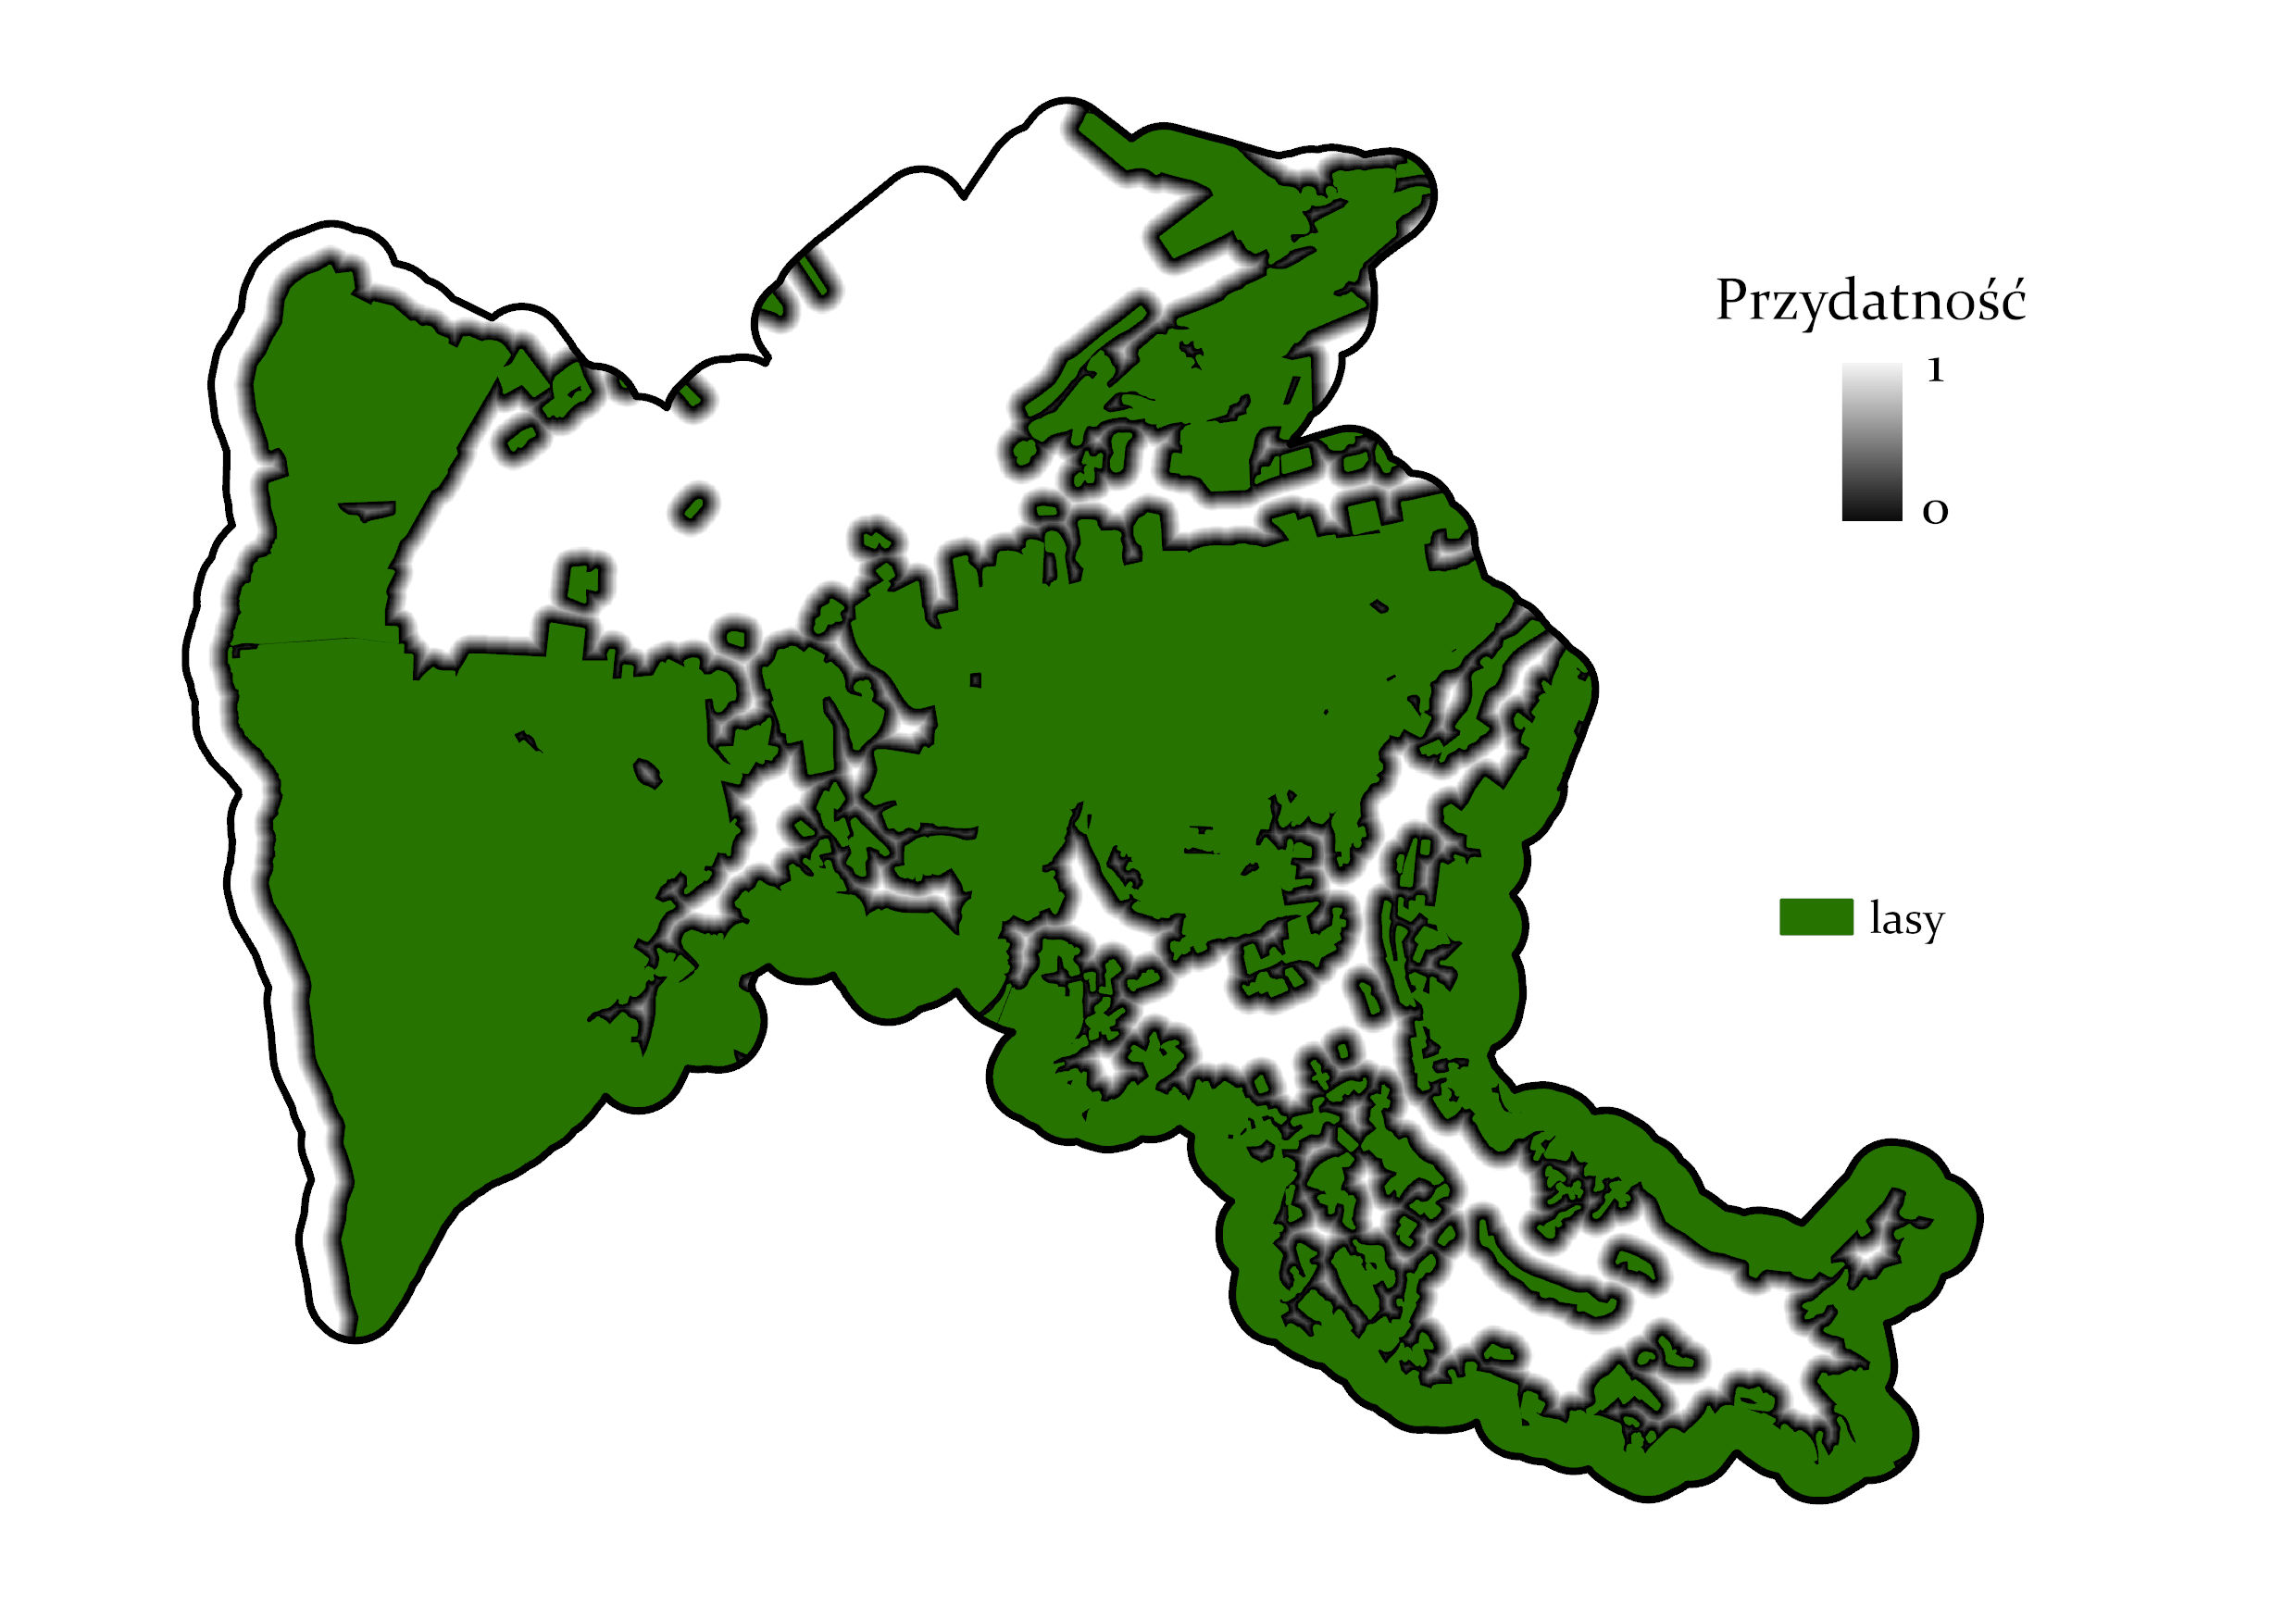
\includegraphics[width=0.75\textwidth]{img/kryterium3-lasy.jpg}
    \caption{Mapa przydatności dla kryterium 3. zawierająca lasy}
\end{figure}
\vspace{10pt}


\subsection{Kryterium 4: dostęp do dróg utwardzonych}
Drogi pobrano z bazy BDOT10k, wybierając obiekty o klasie OT\_SKDR\_L. Ze wszystkich dróg wybrano jedynie te utwardzone, tj. których materiał nawierzchni to beton, bruk, kostka kamienna, kostka prefabrykowana, masa bitumiczna lub płyty betonowe.
\vspace{5pt}

\begin{mintedbox}{python}
drogi_utwardzone = arcpy.analysis.Select(drogi, 'drogi_utwardzone', "MATE_NAWIE IN ('beton', 'bruk', 'kostka kamienna', 'kostka prefabrykowana', 'masa bitumiczna', 'płyty betonowe')")
\end{mintedbox}
\vspace{10pt}

Korzystając z narzędzia \textit{LineDensity} utworzono raster z gęstością dróg utwardzonych na km².
\vspace{5pt}

\begin{mintedbox}{python}
density = arcpy.sa.LineDensity(
    in_polyline_features=drogi_utwardzone,
    population_field=None,
    cell_size=5,
    search_radius=1000,
    area_unit_scale_factor="SQUARE_KILOMETERS",
)
\end{mintedbox}
\vspace{10pt}

Aby móc uzależnić funkcję reklasyfikacyjną od wartości rastra, liczy się maksymalna wartość gęstości dróg w obszarze.
\vspace{5pt}

\begin{mintedbox}{python}
arcpy.management.CalculateStatistics(density)
max_value = density.maximum
\end{mintedbox}
\vspace{10pt}

Zostaje dokonana reklasyfikacja zgodnie z funkcją liniową. Wartości gęstości od 0 do 30\% przyjmują zerową przydatność, od 30\% do 70\% liniowo rosną do maksymalnej przydatności, od 70\% w górę przyjmując maksymalną przydatność.
\vspace{5pt}

\begin{mintedbox}{python}
kryterium_4 = arcpy.sa.RescaleByFunction(
    in_raster=density,
    transformation_function=f"LINEAR {0.3 * max_value} {0.7 * max_value}",
    from_scale=0,
    to_scale=1   
)
\end{mintedbox}
\vspace{10pt}

Reklasyfikacji dokonano zgodnie z funkcją przedstawioną poniżej.
\vspace{5pt}

\begin{figure}[H]
    \centering
    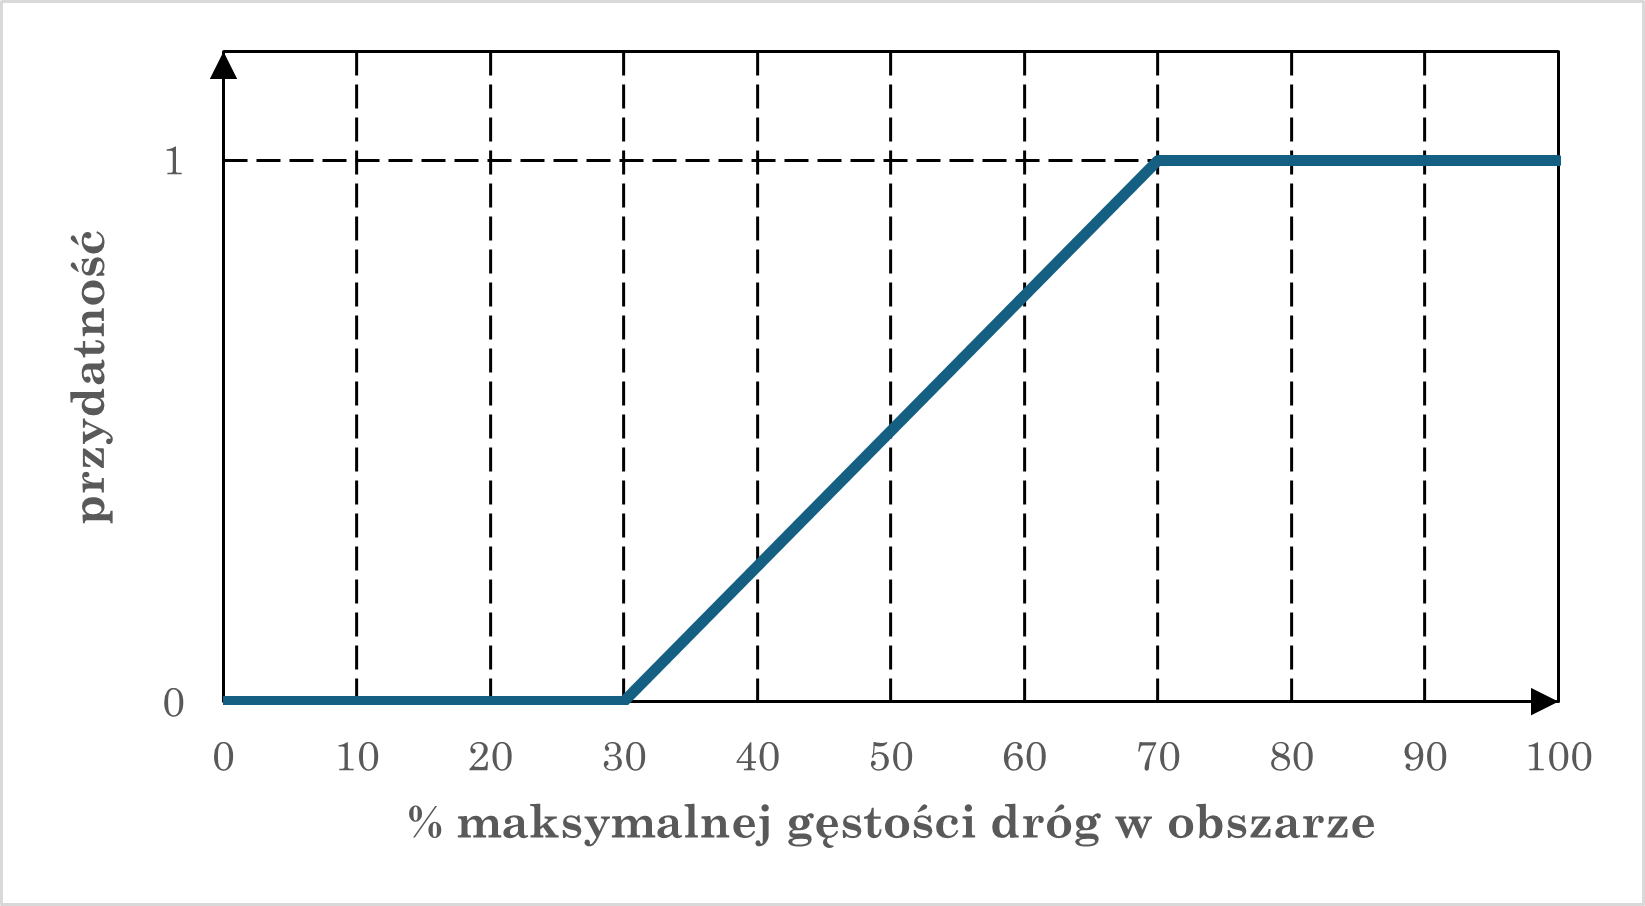
\includegraphics[width=0.6\textwidth]{img/kryterium4-wykres-glowny.png}
    \caption{Reklasyfikacja dla kryterium 4.}
\end{figure}

% \begin{mintedbox}{python}
% kryterium_4.save(f'{geobaza}\\kryterium_4')
% \end{mintedbox}

% \begin{figure}[H]
%     \centering
%     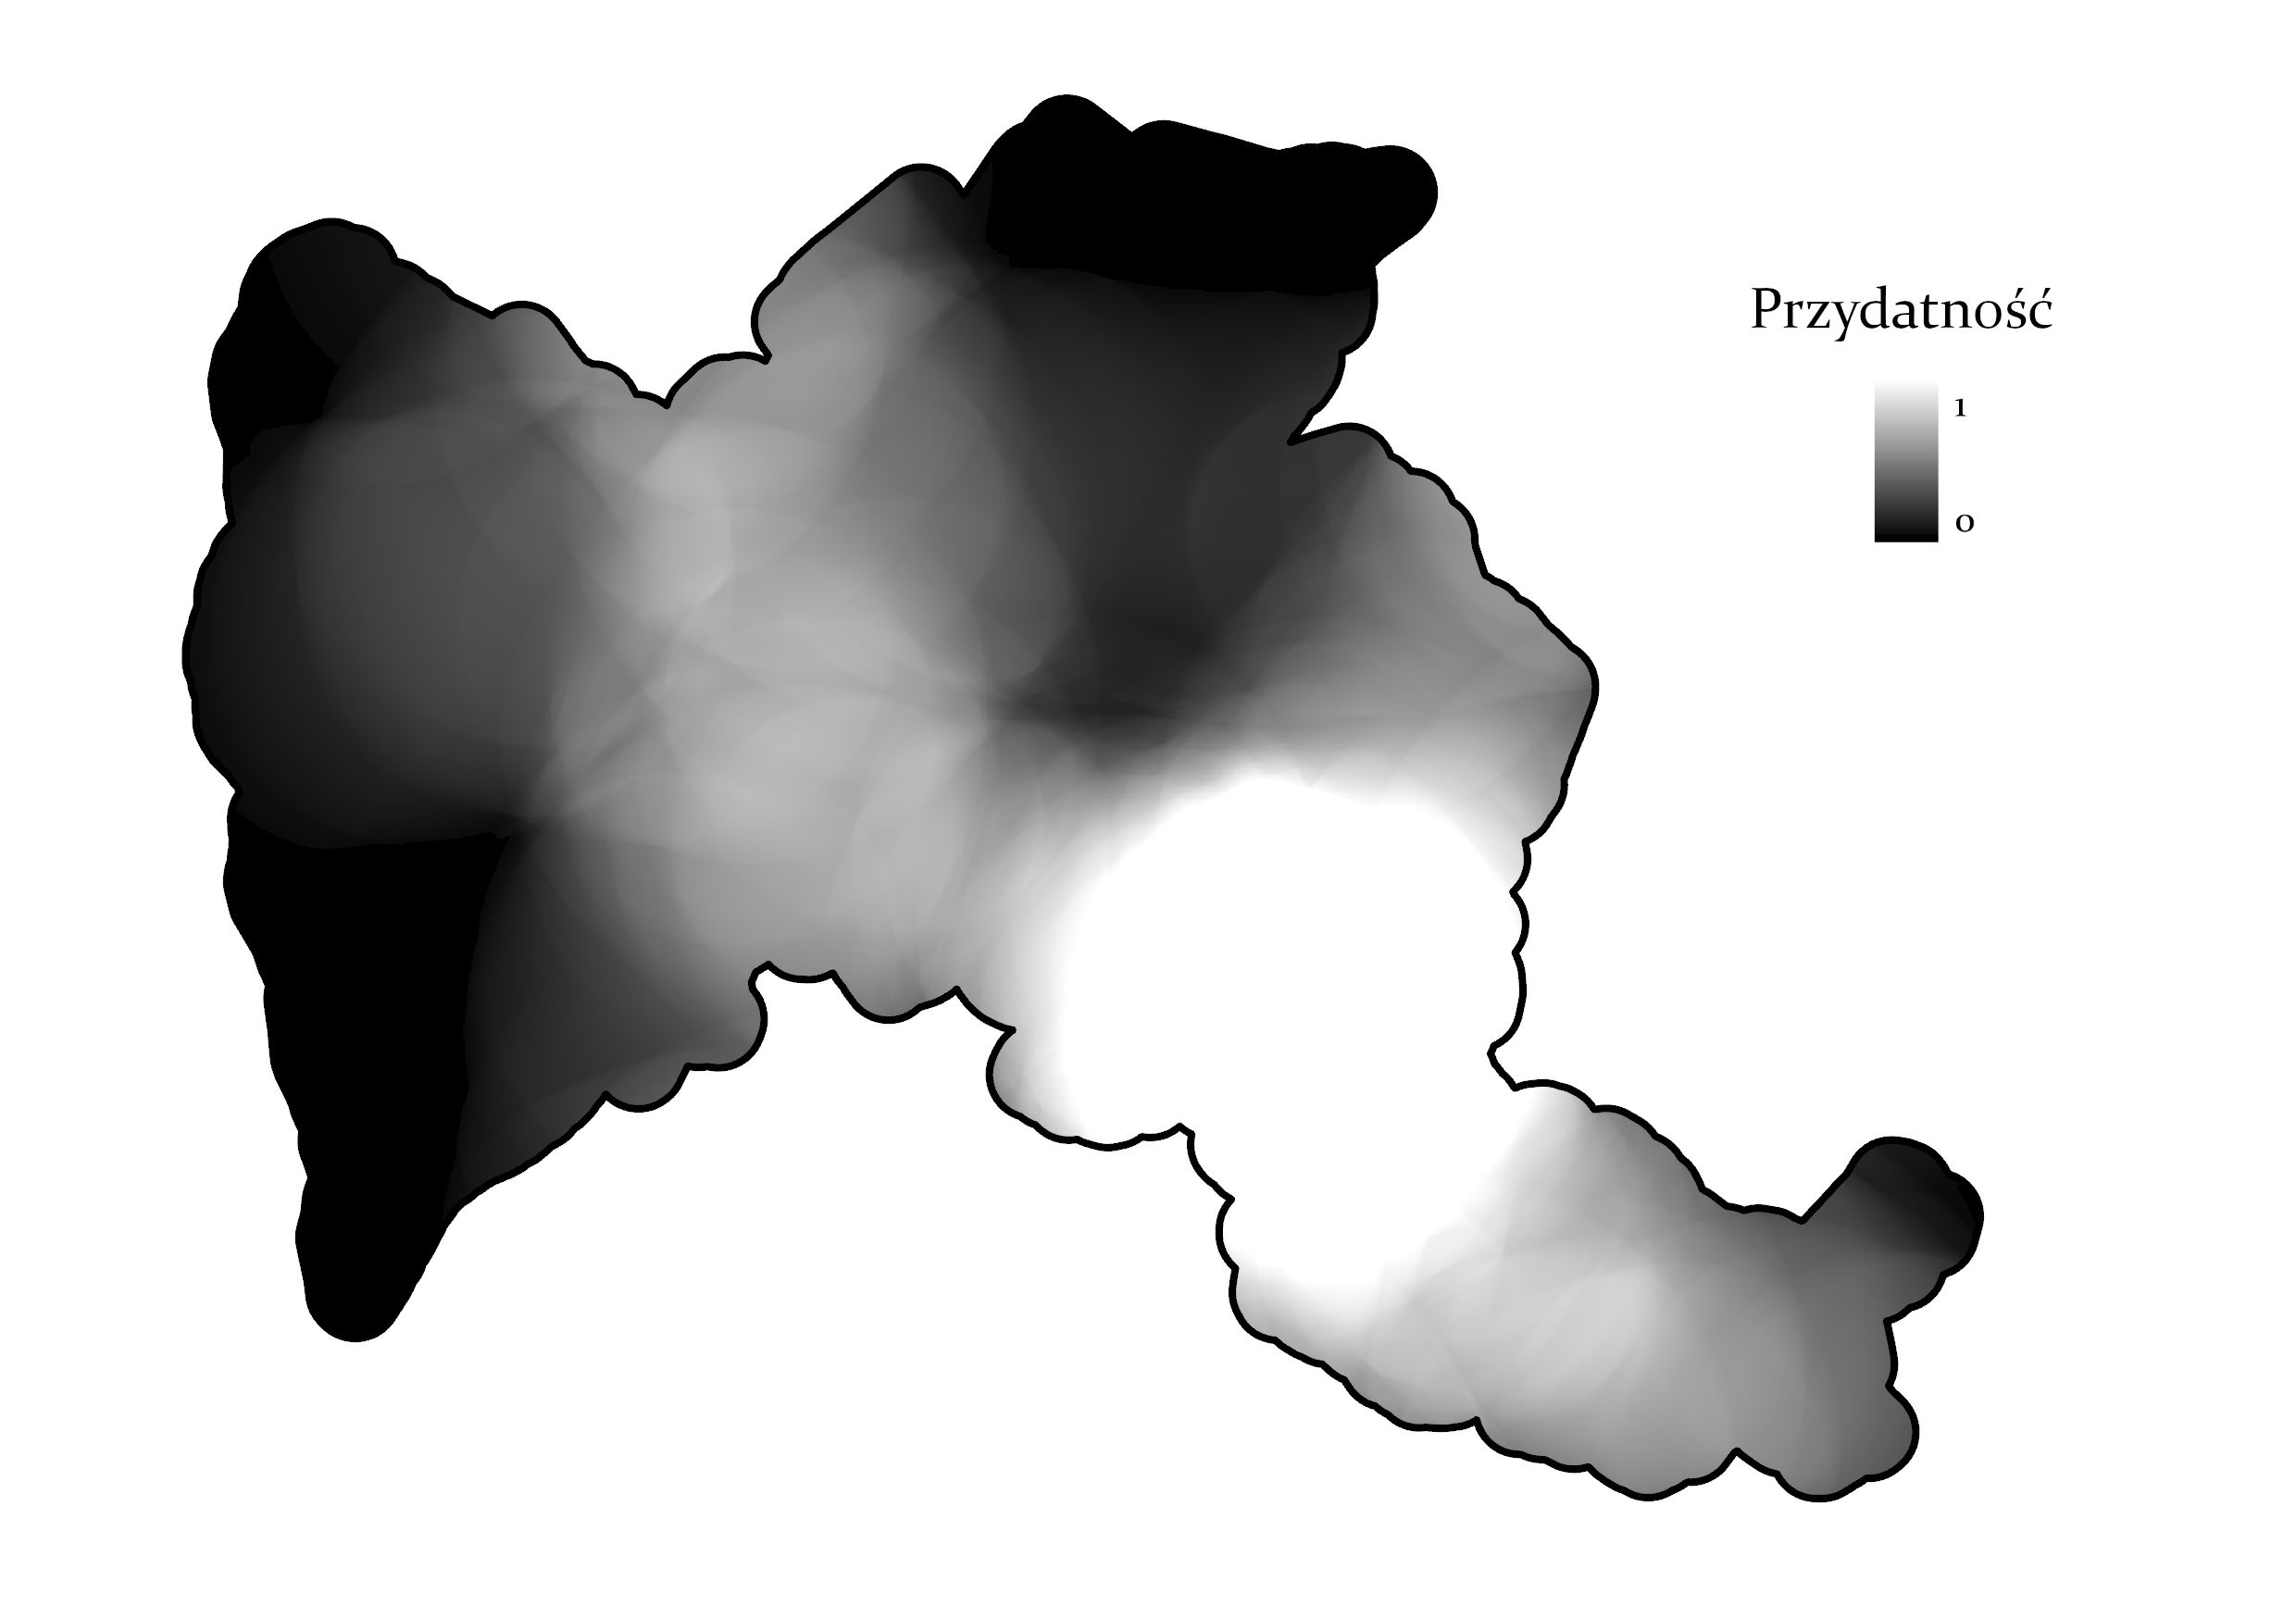
\includegraphics[width=0.75\textwidth]{img/kryterium4-layout.jpg}
%     \caption*{Mapa przydatności dla kryterium 4.}
% \end{figure}

% \begin{figure}[H]
%     \centering
%     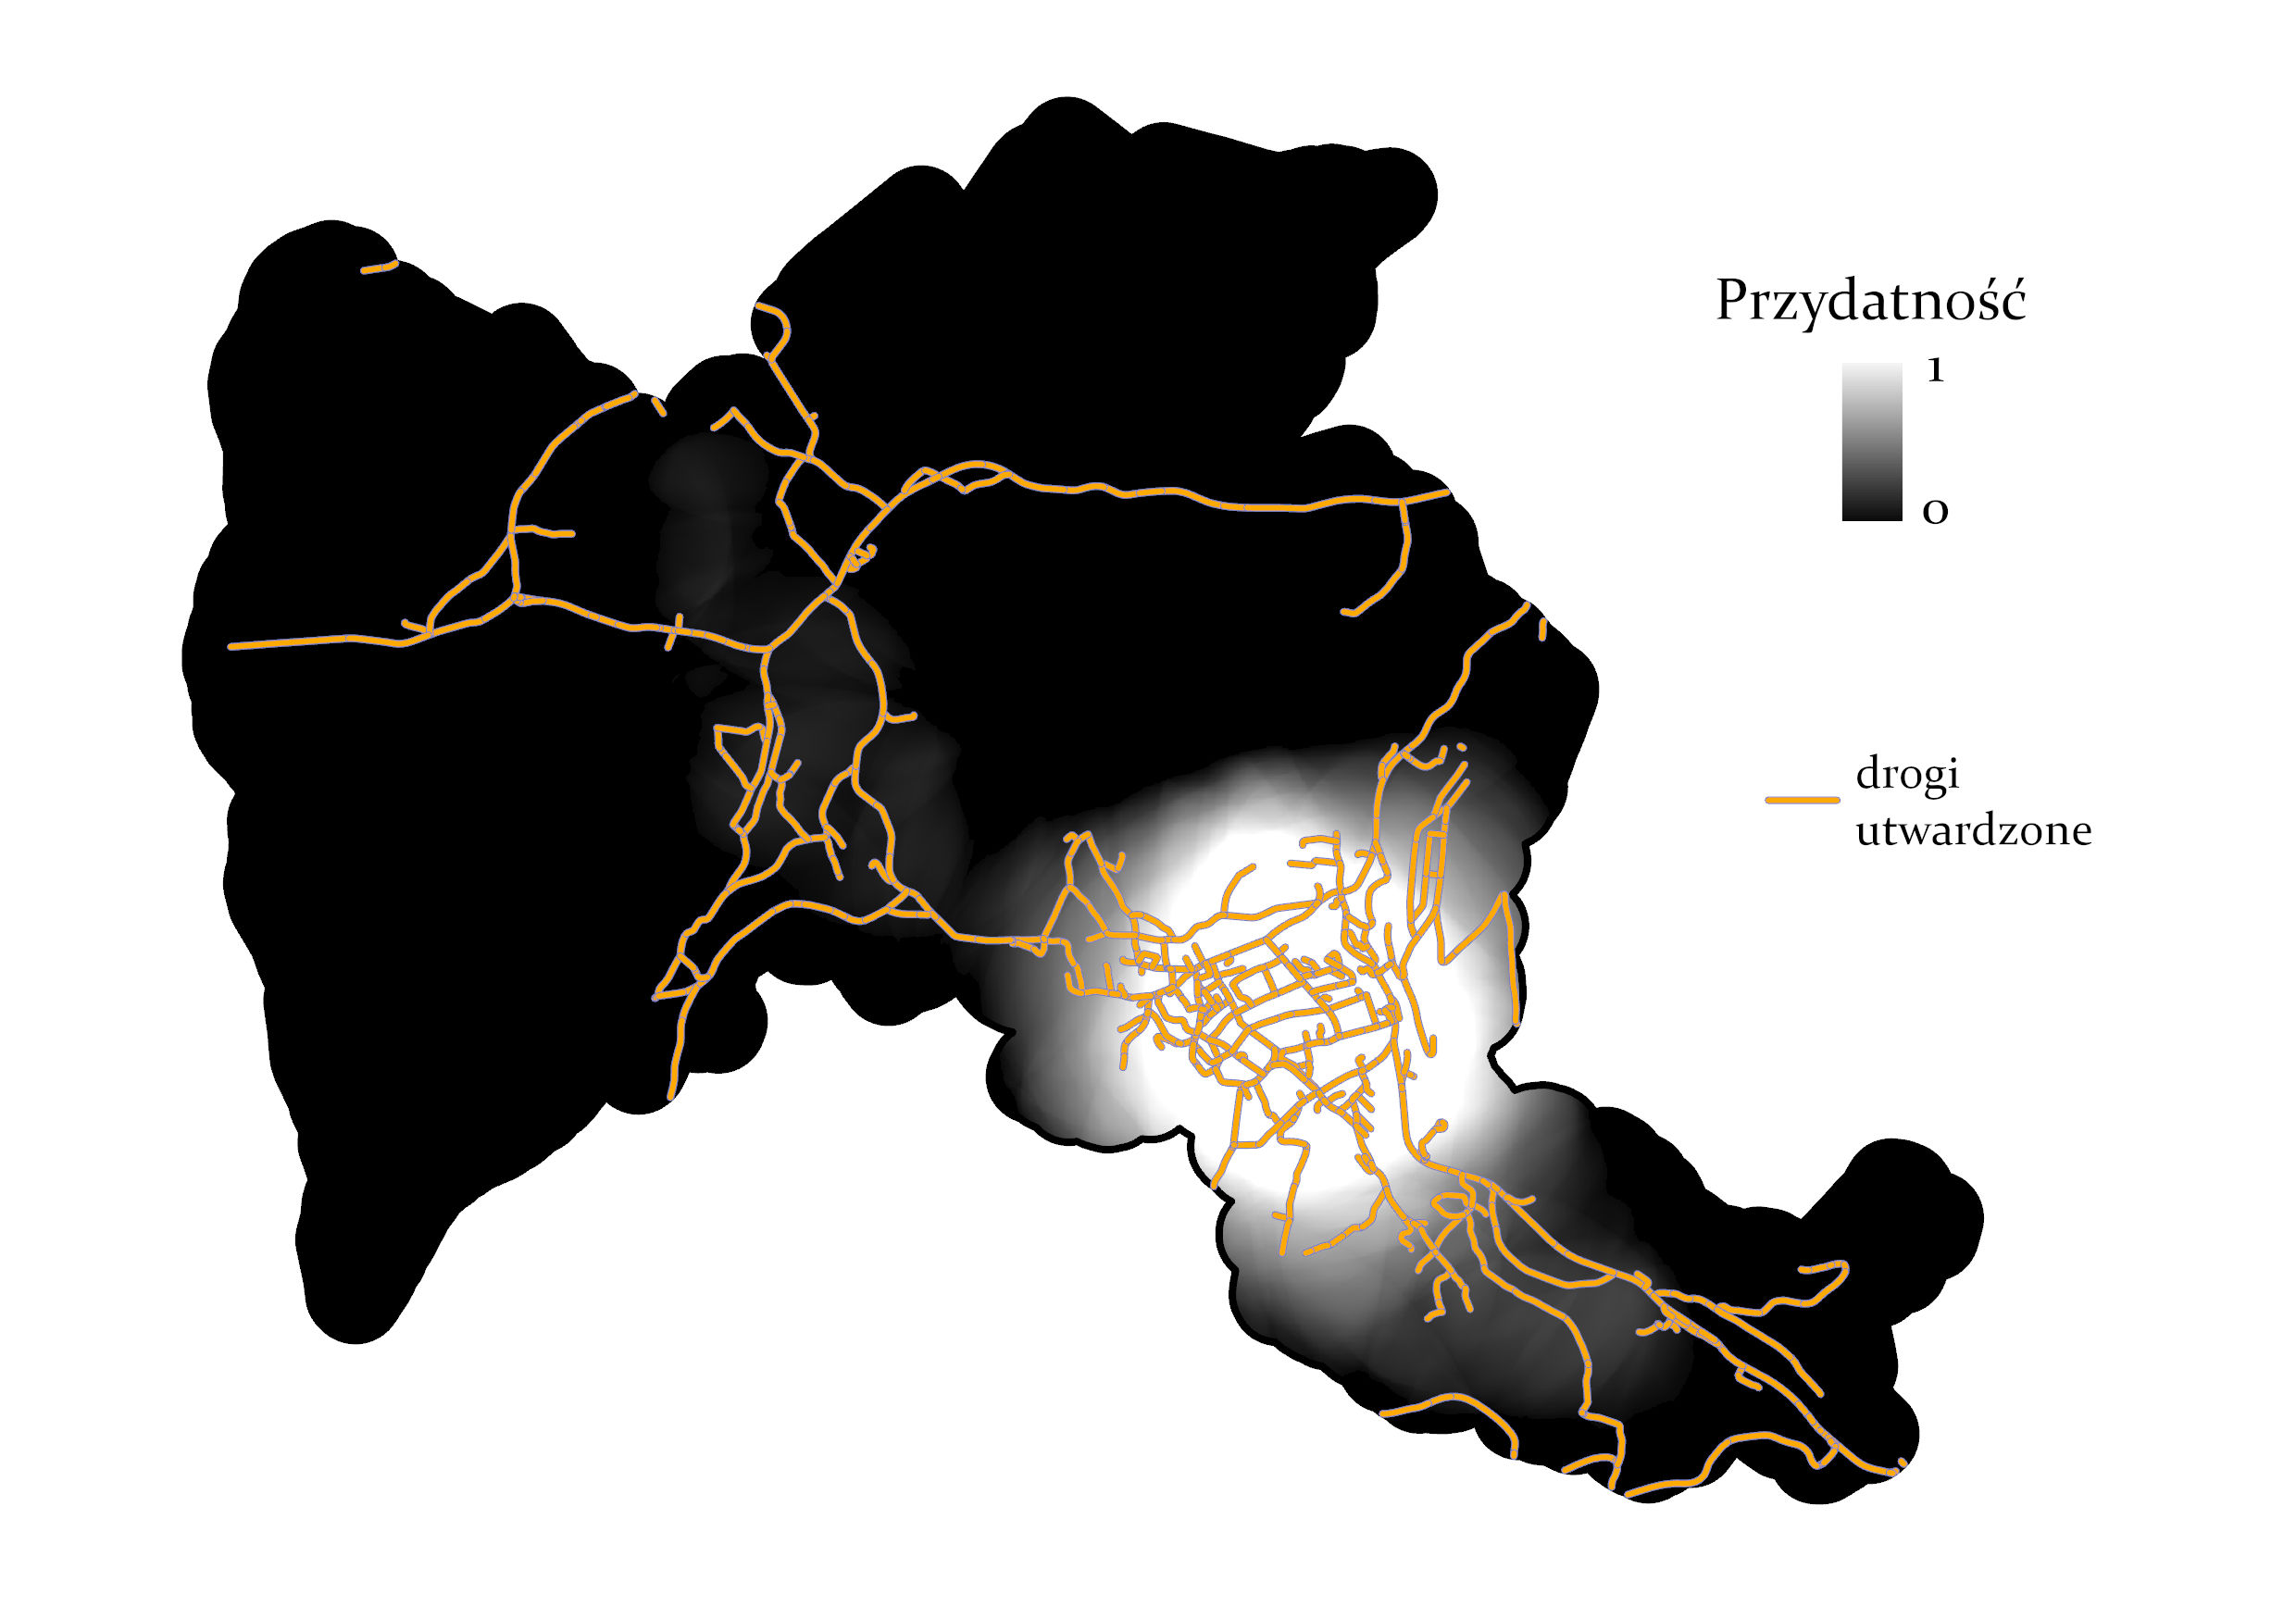
\includegraphics[width=0.75\textwidth]{img/kryterium4-drogi.jpg}
%     \caption*{Mapa przydatności dla kryterium 4. zawierająca drogi utwardzone}
% \end{figure}
\vspace{10pt}

\subsection{Kryterium 5: nachylenie stoków}
W celu realizacji kryterium pobrano kafelki NMT dla obszaru gminy. Połączono je z użyciem narzędzia \textit{Mosaic To New Raster}. Dla nowo powstałego rastra obliczono procentowe nachylenia stoków z użyciem narzędzie \textit{Slope} z zestawu \textit{3D Analyst}.
\vspace{5pt}

\begin{mintedbox}{python}
arcpy.ddd.Slope(nmt, "slope", "PERCENT_RISE", 1)
\end{mintedbox}
\vspace{10pt}

\begin{figure}[H]
    \centering
    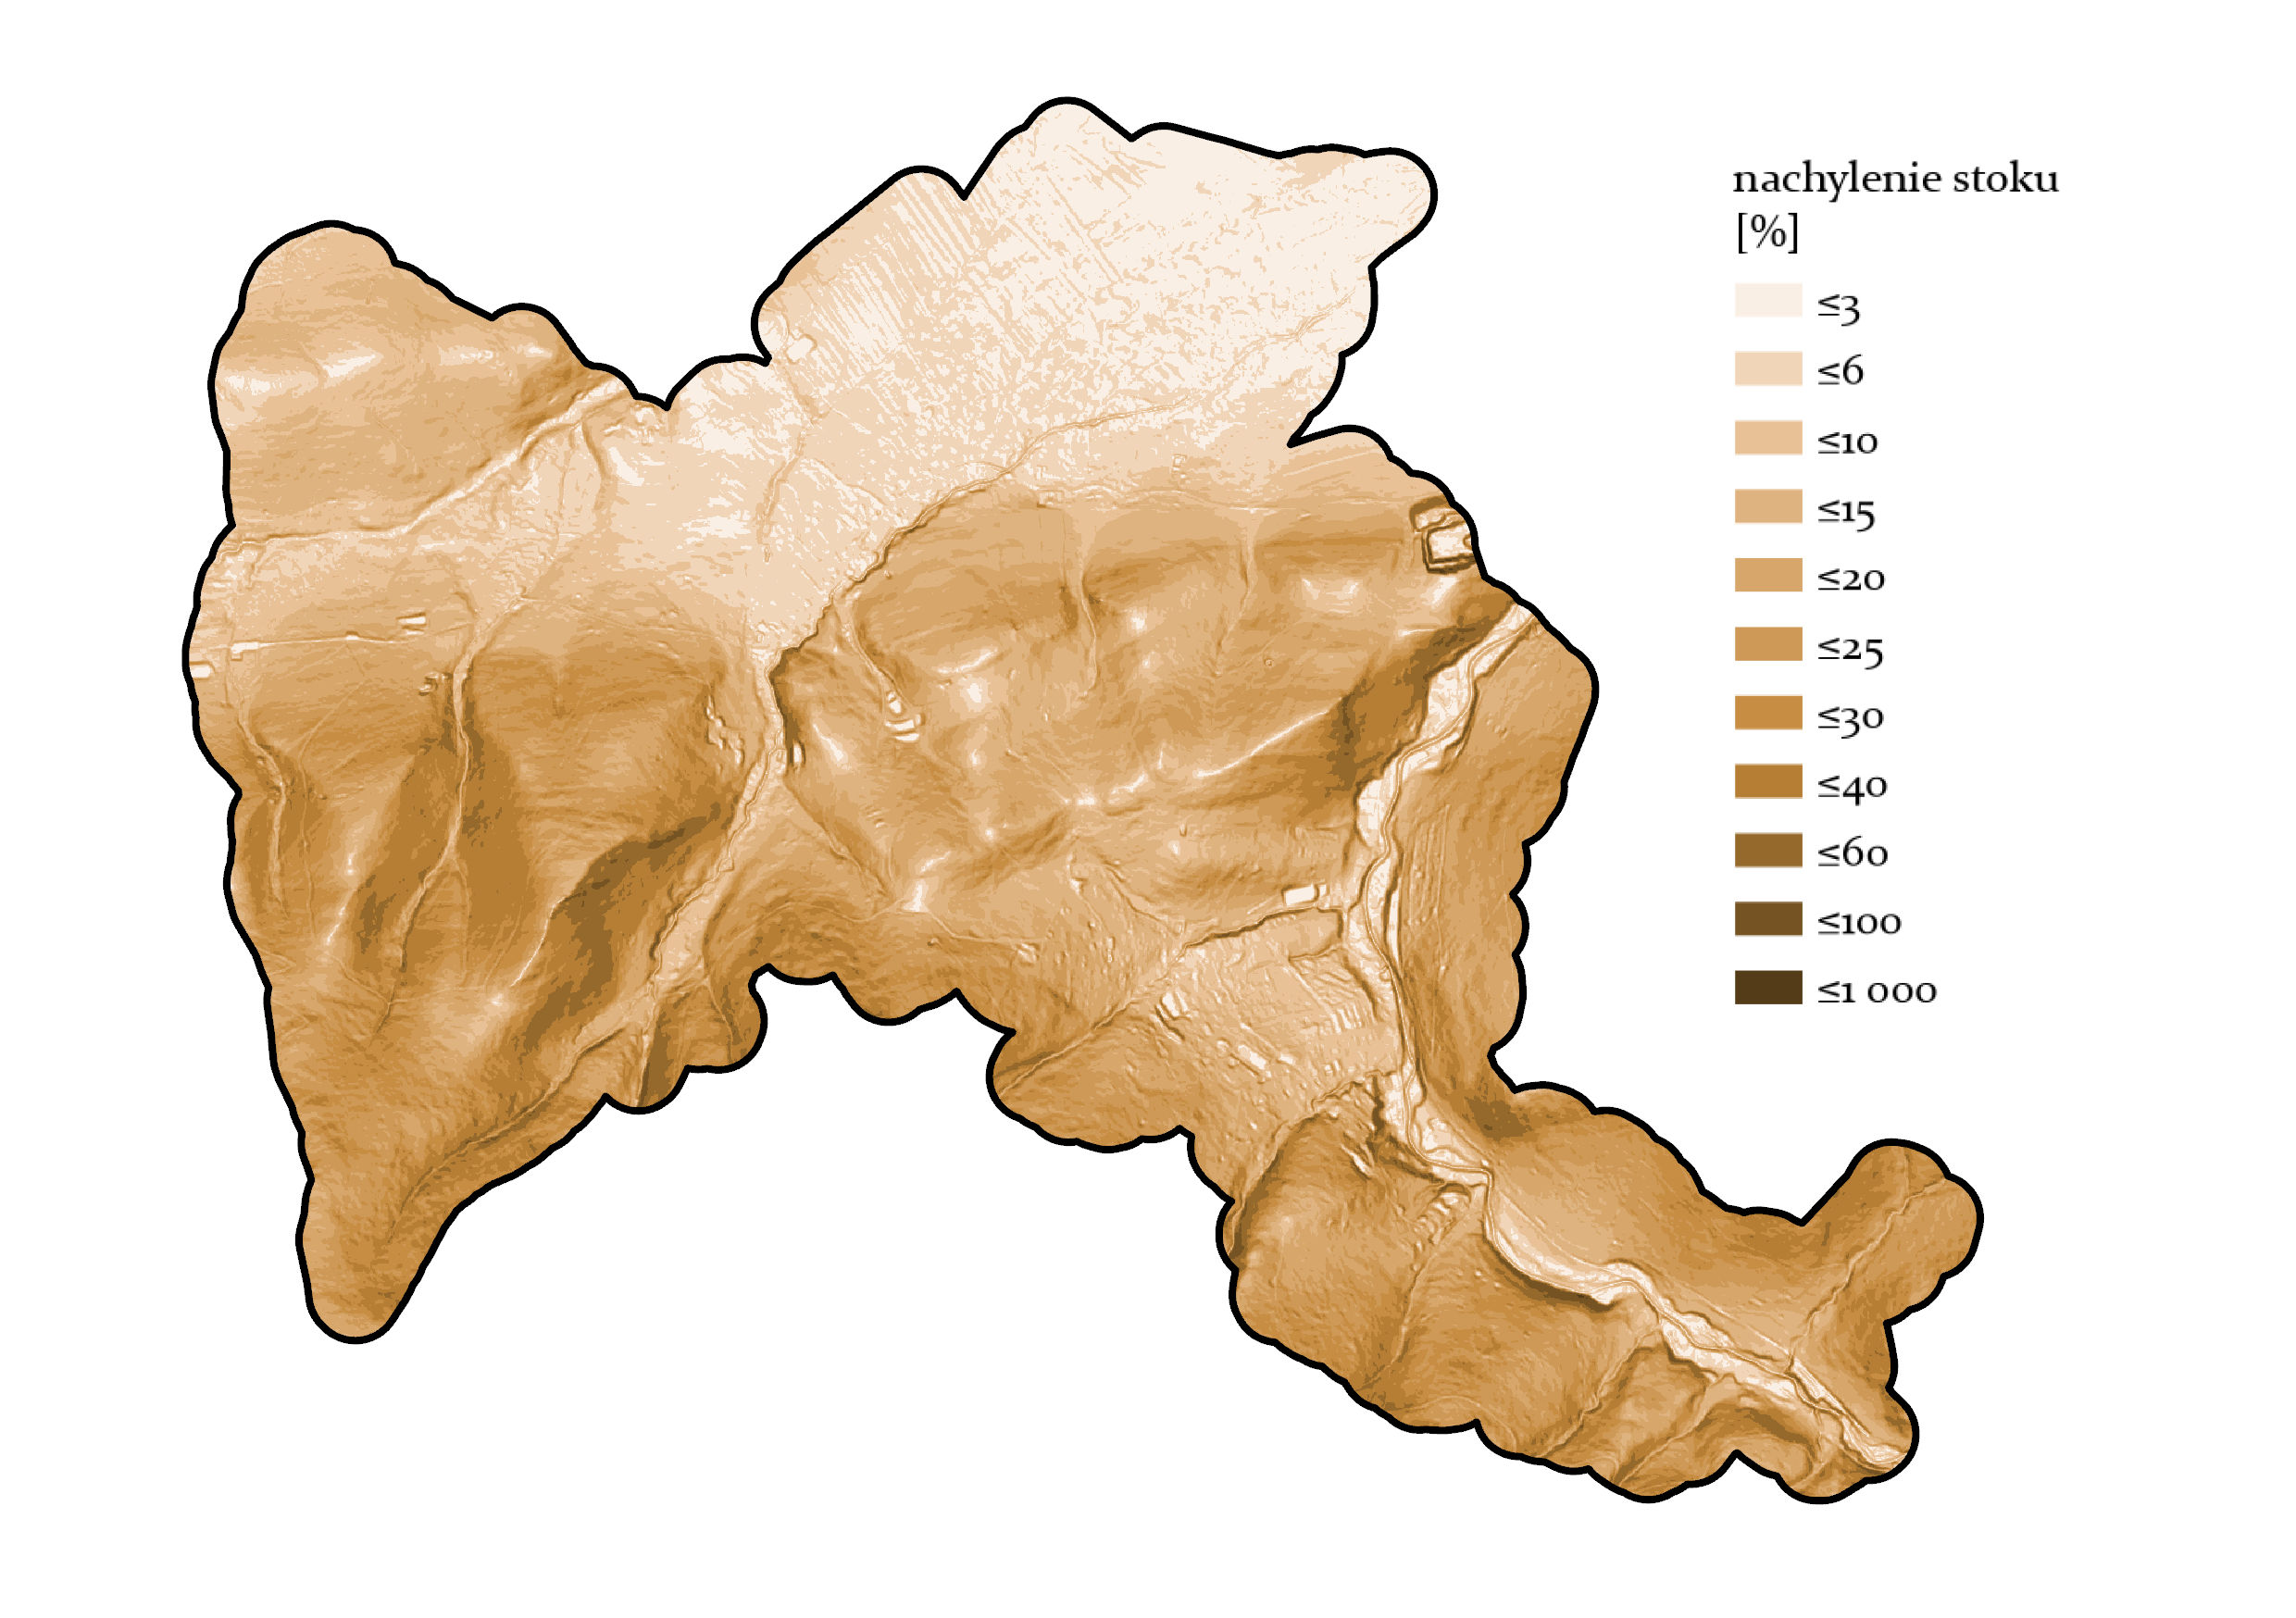
\includegraphics[width=0.6\textwidth]{img/kryterium5-stoki.jpg}
    \caption{Mapa nachyleń stoków powstała z użyciem narzędzie \textit{Slope}}
\end{figure}

Powstały raster zreklasyfikowano, przyporządkowując stokom o nachyleniu od 0 do 7\% maksymalną przydatność, od 7 do 10 \% stopniowo spadając, przyjmując dla stoków o nachyleniu powyżej 10\% zerową przydatność.
\vspace{5pt}

\begin{mintedbox}{python}
slope_fuzzy = arcpy.sa.FuzzyMembership("slope", fuzzy_function="LINEAR 10 7")
\end{mintedbox}
\vspace{10pt}

Reklasyfikacji dokonano zgodnie z funkcją przedstawioną poniżej.
\vspace{5pt}

\begin{figure}[H]
    \centering
    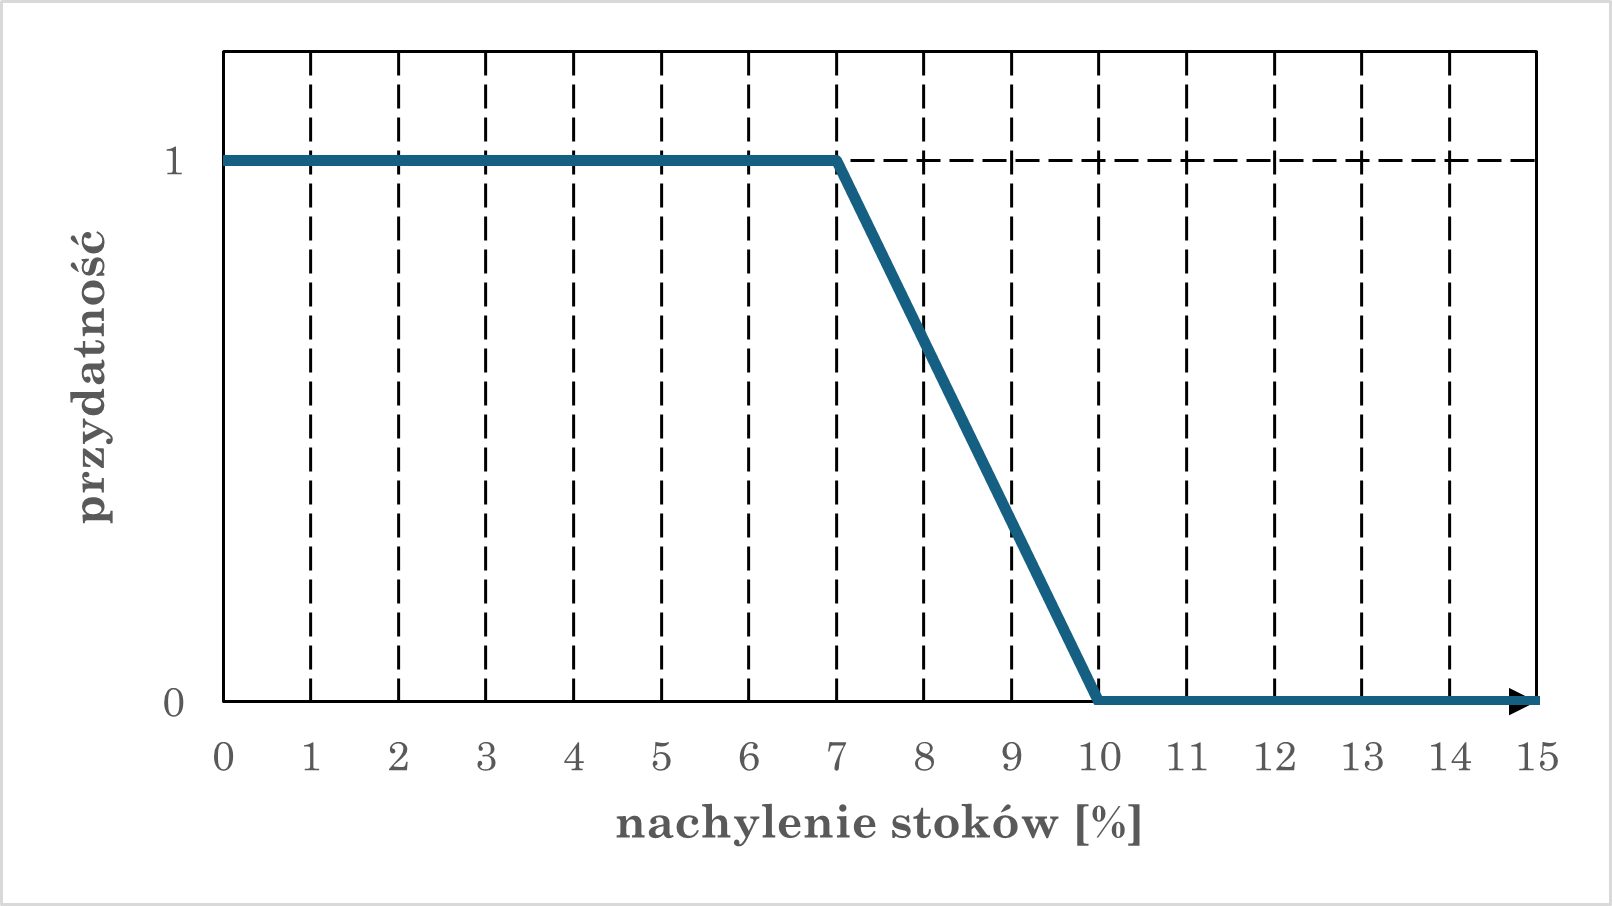
\includegraphics[width=0.6\textwidth]{img/kryterium5-wykres-glowny.png}
    \caption{Reklasyfikacja dla kryterium 5.}
\end{figure}
\vspace{10pt}

Kryterium eliminuje dużą część obszaru ze względu na dużą górzystość terenu. Przydatna pozostaje północna i północno-wschodnia część gminy oraz niewielkie obszary w pozostałej części gminy.
\vspace{5pt}

\begin{figure}[H]
    \centering
    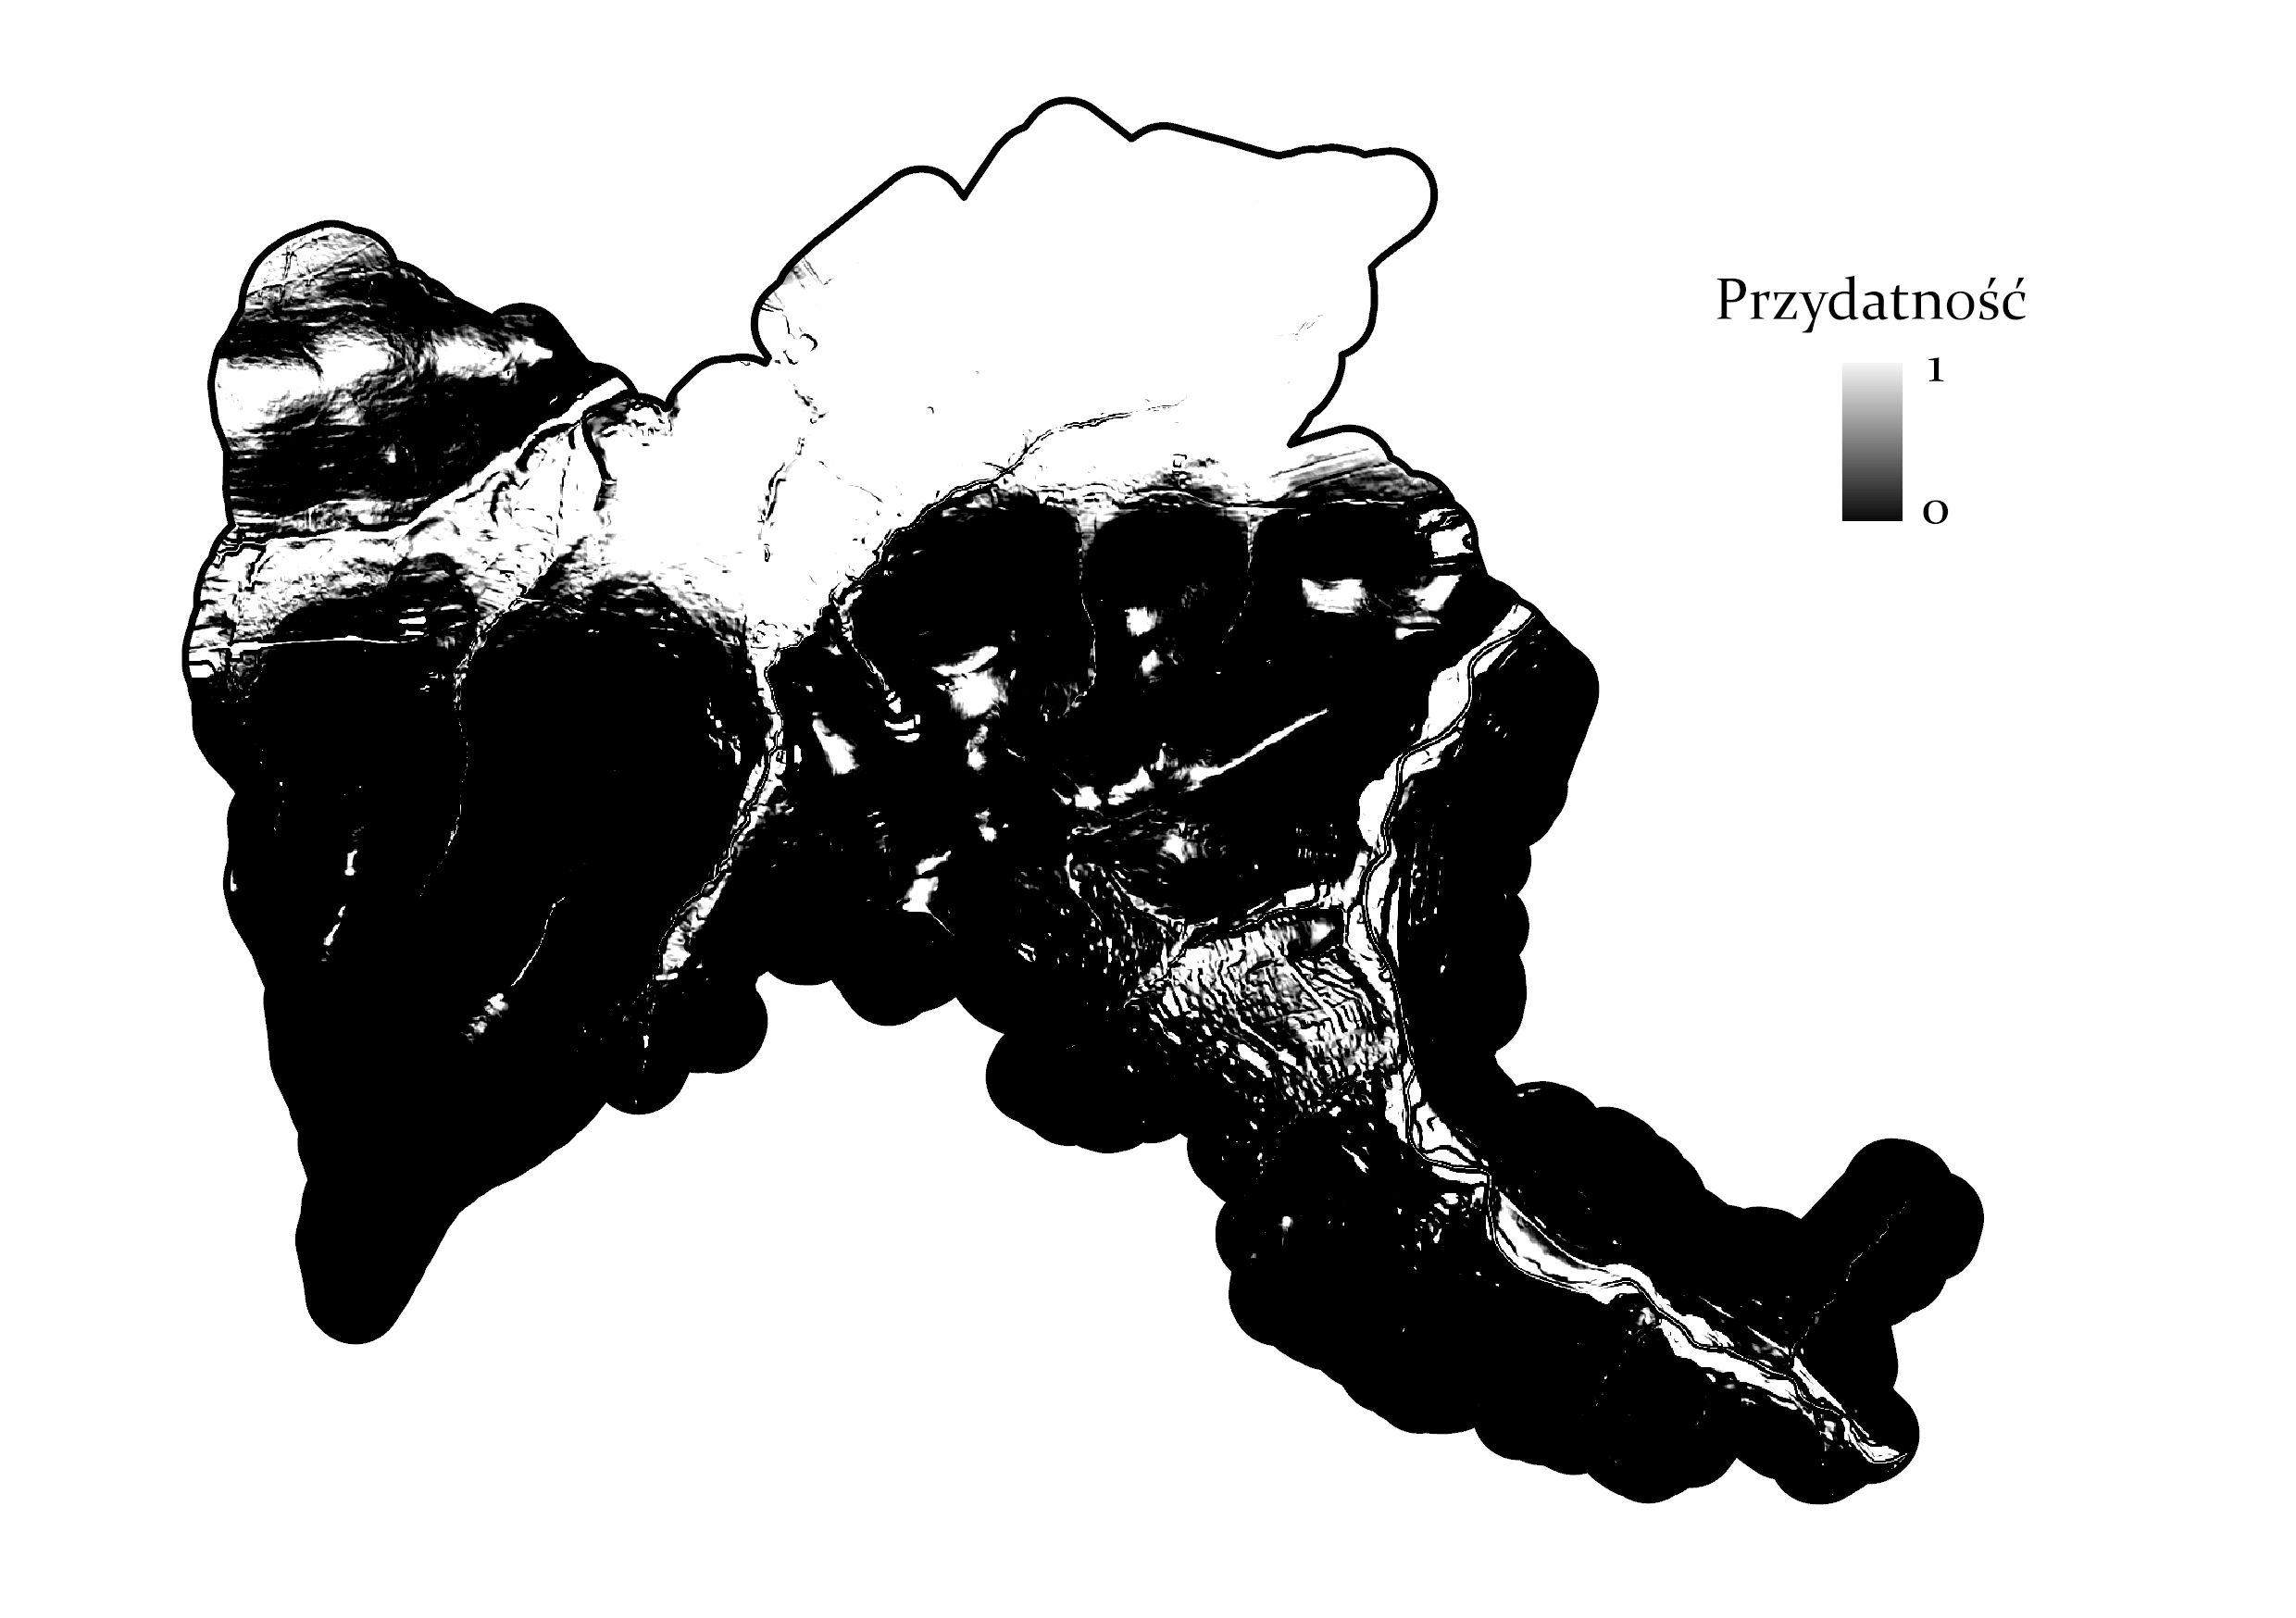
\includegraphics[width=0.75\textwidth]{img/kryterium5-layout.jpg}
    \caption{Mapa przydatności dla kryterium 5.}
\end{figure}
\vspace{10pt}

Mapę zapisano do geobazy w celu użycia w późniejszym etapie.
\vspace{5pt}

\begin{mintedbox}{python}
woda_mapa.save(f'{geobaza}\\kryterium_5')
\end{mintedbox}
\newpage

\subsection{Kryterium 6: dostęp do światła słonecznego}

Do tego kryterium również wykorzystano NMT, a także narzędzie \textit{Aspect} z zestawu \textit{3D Analyst}.
\vspace{5pt}

\begin{mintedbox}{python}
aspect = arcpy.ddd.Aspect(nmt)
\end{mintedbox}
\vspace{10pt}

Efektem działania funkcji był poniższy raster, przedstawiający, na którą stronę świata wystawiony jest stok.
\vspace{5pt}

\begin{figure}[H]
    \centering
    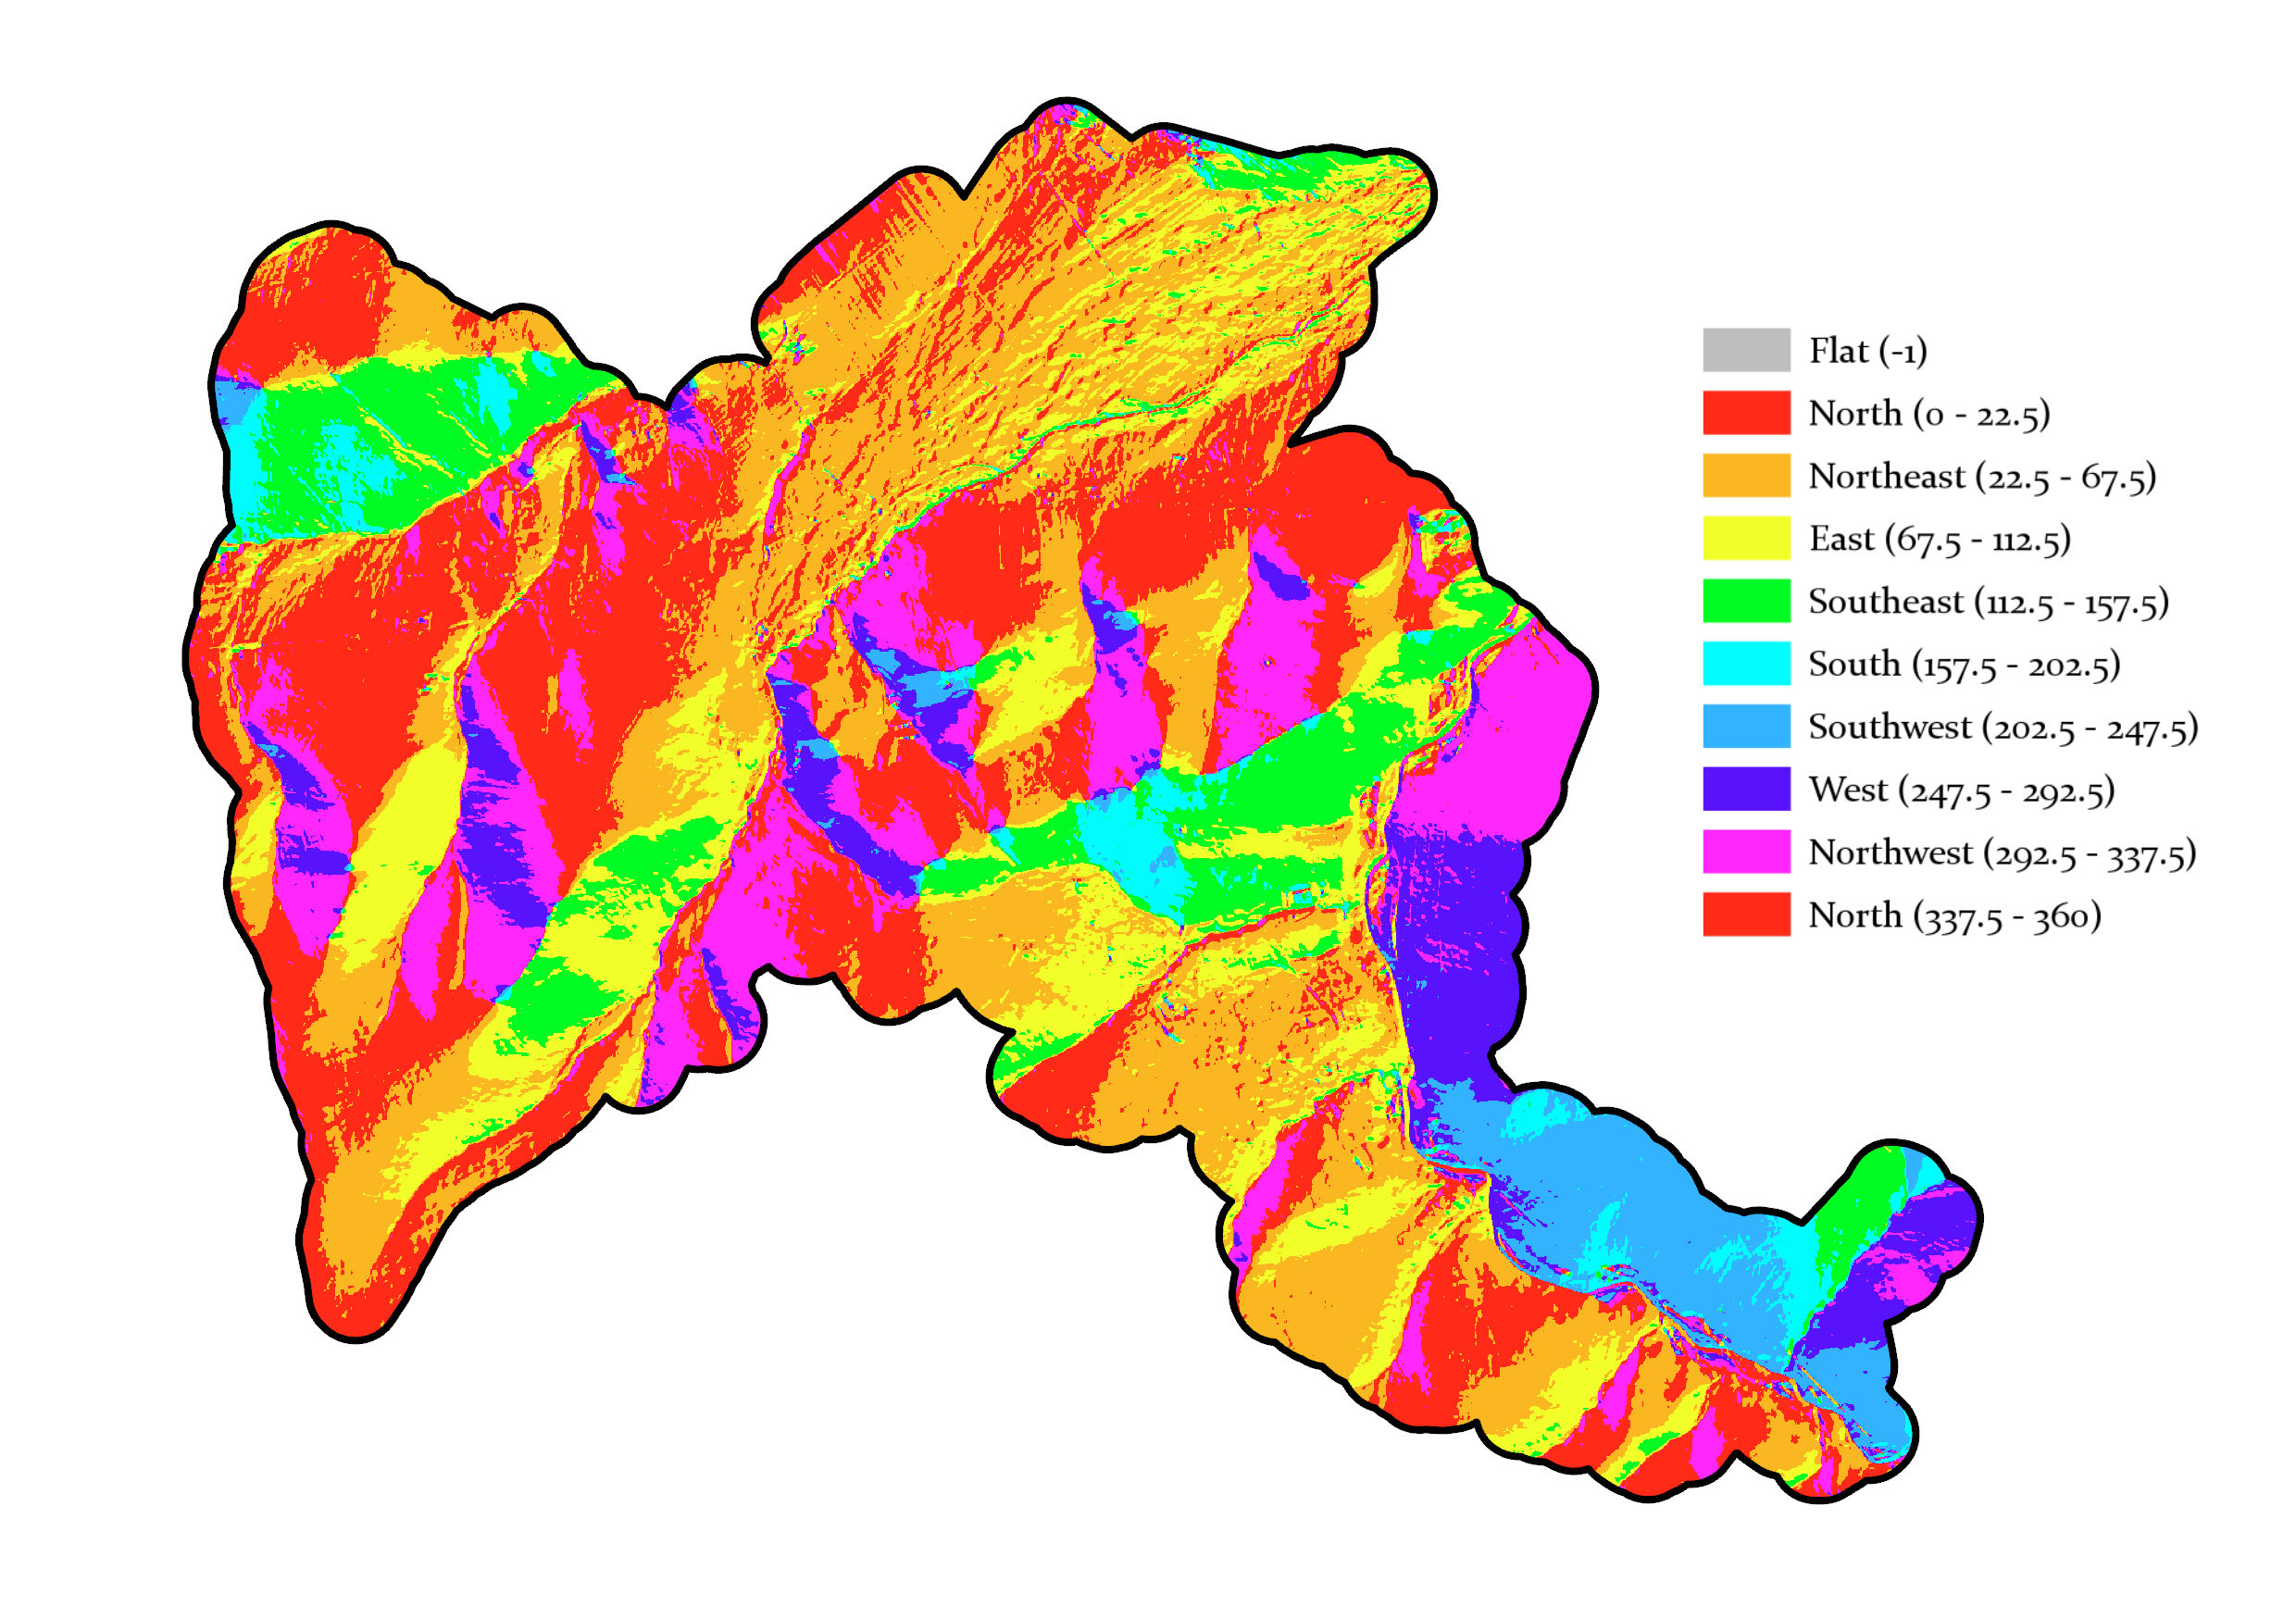
\includegraphics[width=0.75\textwidth]{img/kryterium6-aspect.jpg}
    \caption{Mapa przydatności dla kryterium 6. zawierająca stopień wystawy słonecznej}
\end{figure}
\vspace{10pt}

Przydatne w kontekście naszego projektu są stoki południowo-zachodnie, południowe i południowo-wschodnie. Stworzono więc dwie funkcje reklasyfikacyjne: rosnącą od 90 do 113 stopni oraz malejącą od 248 do 270 stopni. 
\vspace{5pt}

\begin{mintedbox}{python}
aspect_fuzzy = arcpy.sa.FuzzyMembership(aspect, fuzzy_function="LINEAR 90 113")
aspect_fuzzy_1 = arcpy.sa.FuzzyMembership(aspect, fuzzy_function="LINEAR 270 248")
\end{mintedbox}
\vspace{10pt}

\begin{figure}[H]
    \centering
    \begin{minipage}{0.48\textwidth}
        \centering
        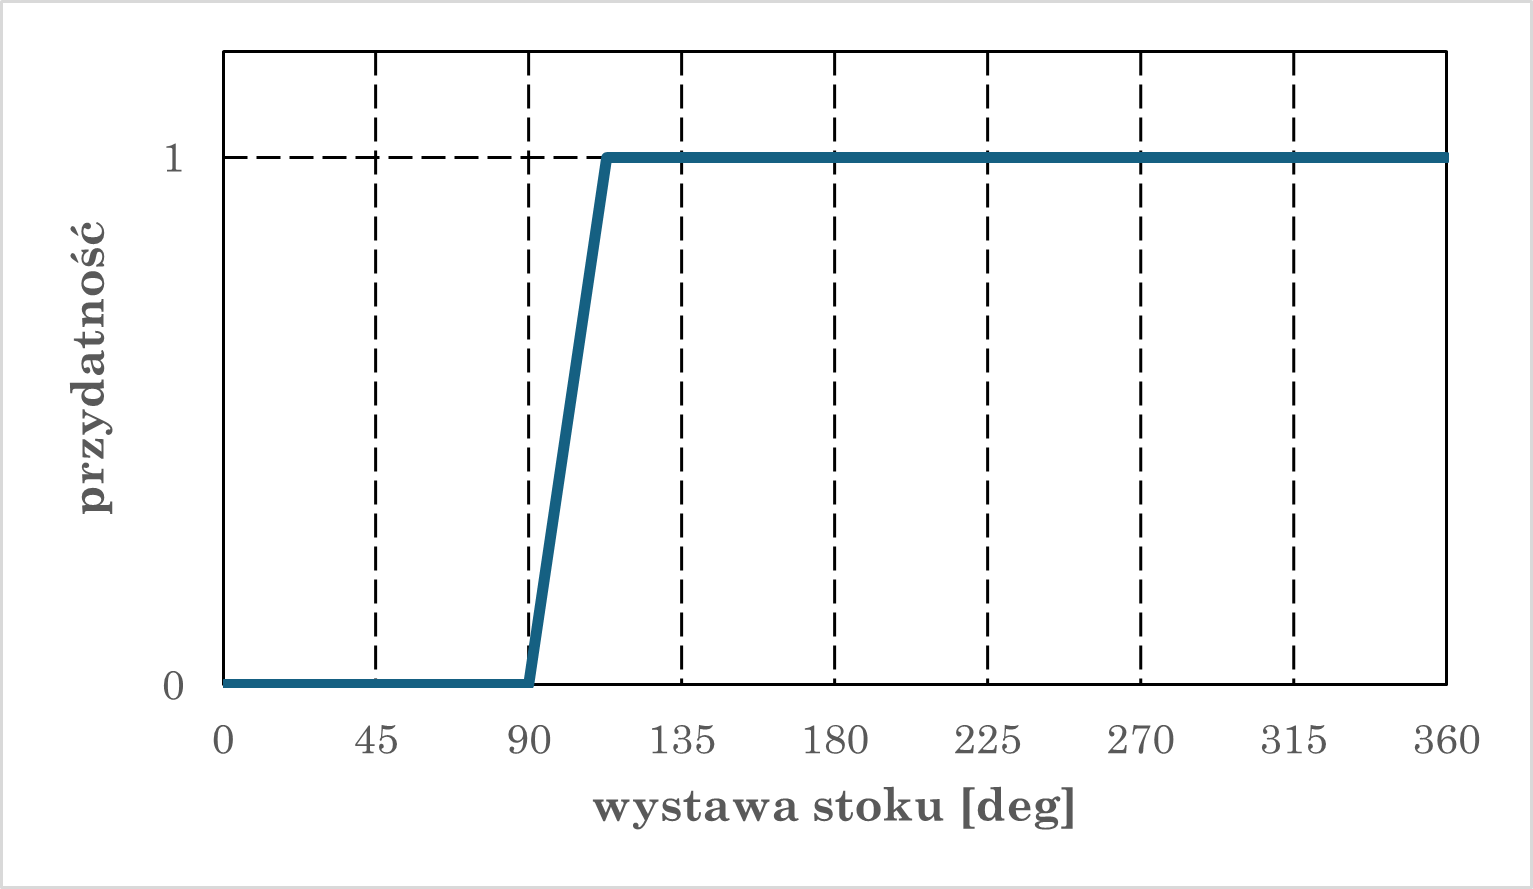
\includegraphics[width=\linewidth]{img/kryterium6-wykres-pierwszy.png}
        \caption{Funkcja rosnąca}
    \end{minipage}
    \begin{minipage}{0.48\textwidth}
        \centering
        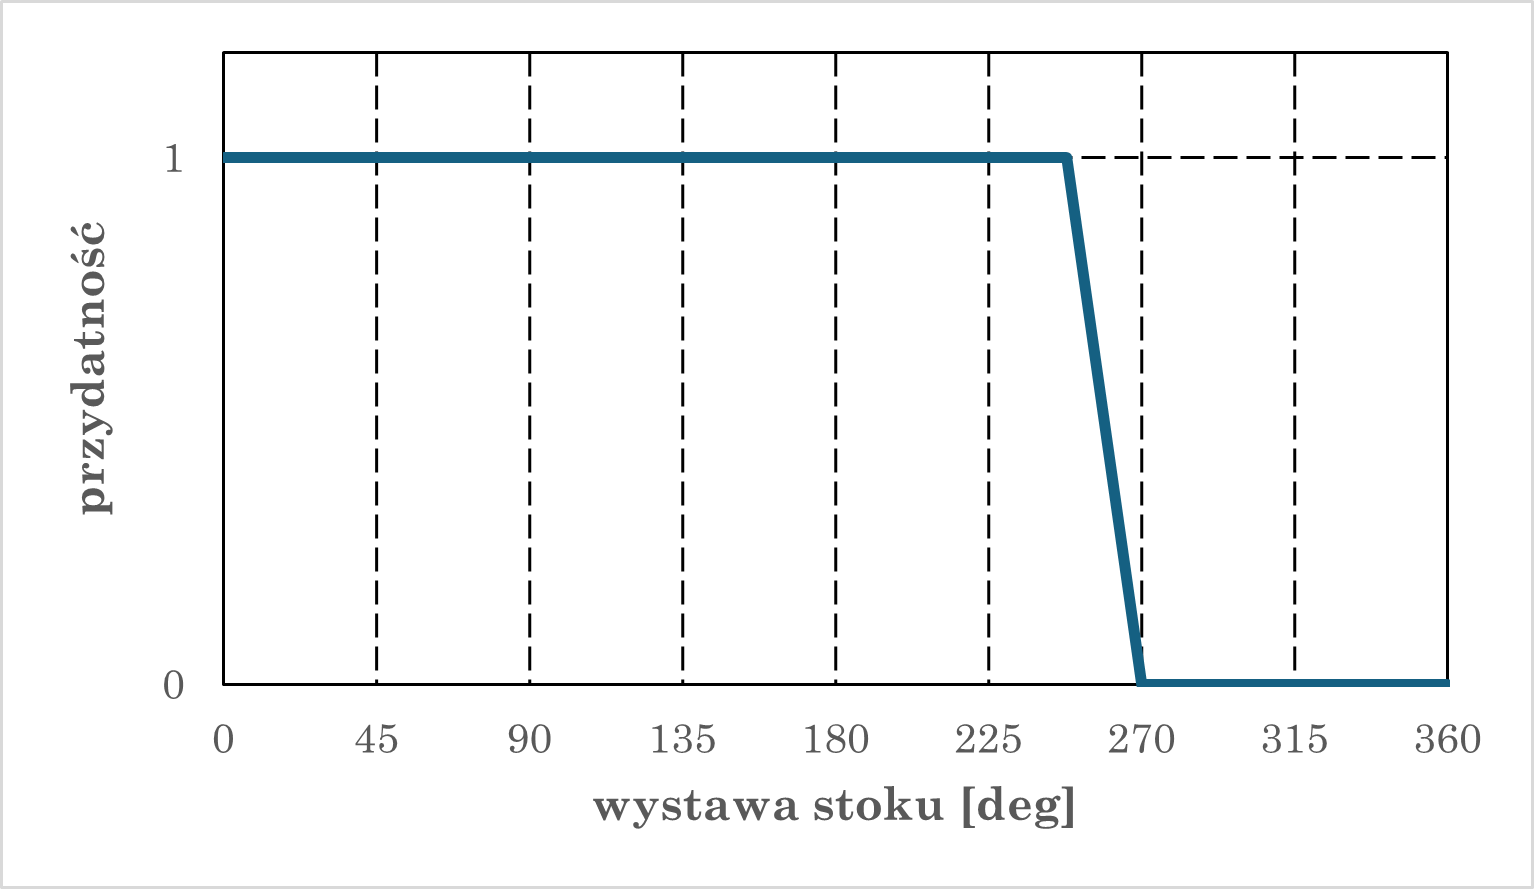
\includegraphics[width=\linewidth]{img/kryterium6-wykres-drugi.png}
        \caption{Funkcja malejąca}
    \end{minipage}
\end{figure}
\newpage

Ostateczny wynik kryterium szóstego uzyskano po połączeniu obu warstw utworzonych wcześniej przy użyciu fuzzy logic. Wykorzystano do tego narzędzie \textit{FuzzyOverlay}.
\vspace{5pt}

\begin{mintedbox}{python}
aspect_overlay = arcpy.sa.FuzzyOverlay([aspect_fuzzy, aspect_fuzzy_1], 'AND')
\end{mintedbox}
\vspace{5pt}

\begin{figure}[H]
    \centering
    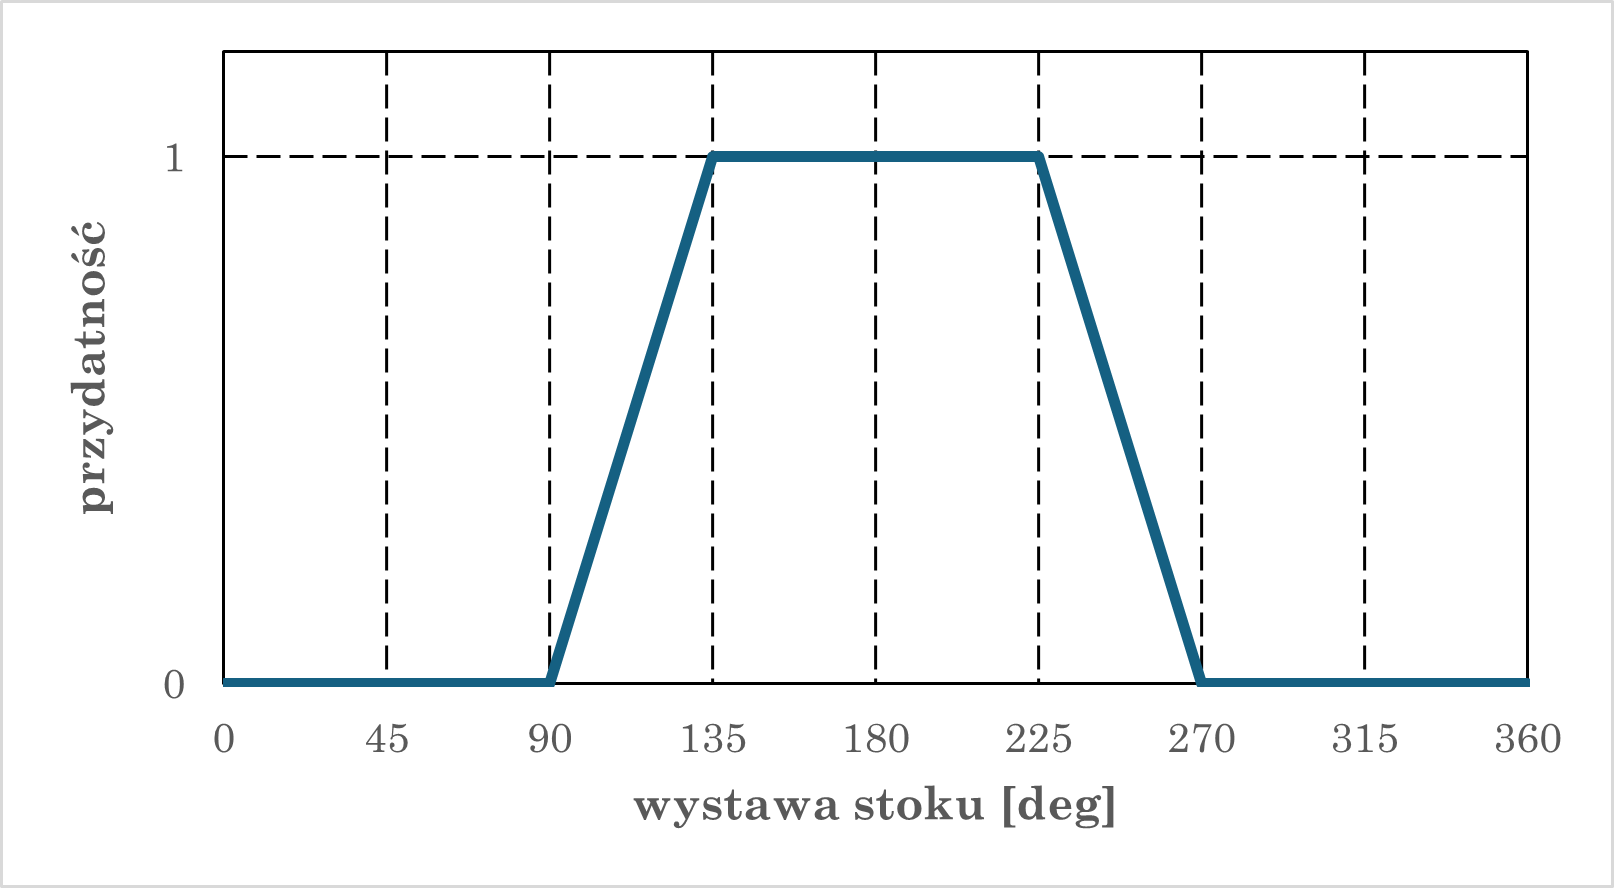
\includegraphics[width=0.7\textwidth]{img/kryterium6-wykres-glowny.png}
    \caption{Reklasyfikacja dla kryterium 6.}
\end{figure}
\vspace{10pt}

Kryterium wyłoniło tereny przydatne w północno-zachodniej, środkowej oraz południowo-wschodniej części obszaru. Znaczna część terenów charakteryzuje się niekorzystną wystawą słoneczną.
\vspace{5pt}

\begin{figure}[H]
    \centering
    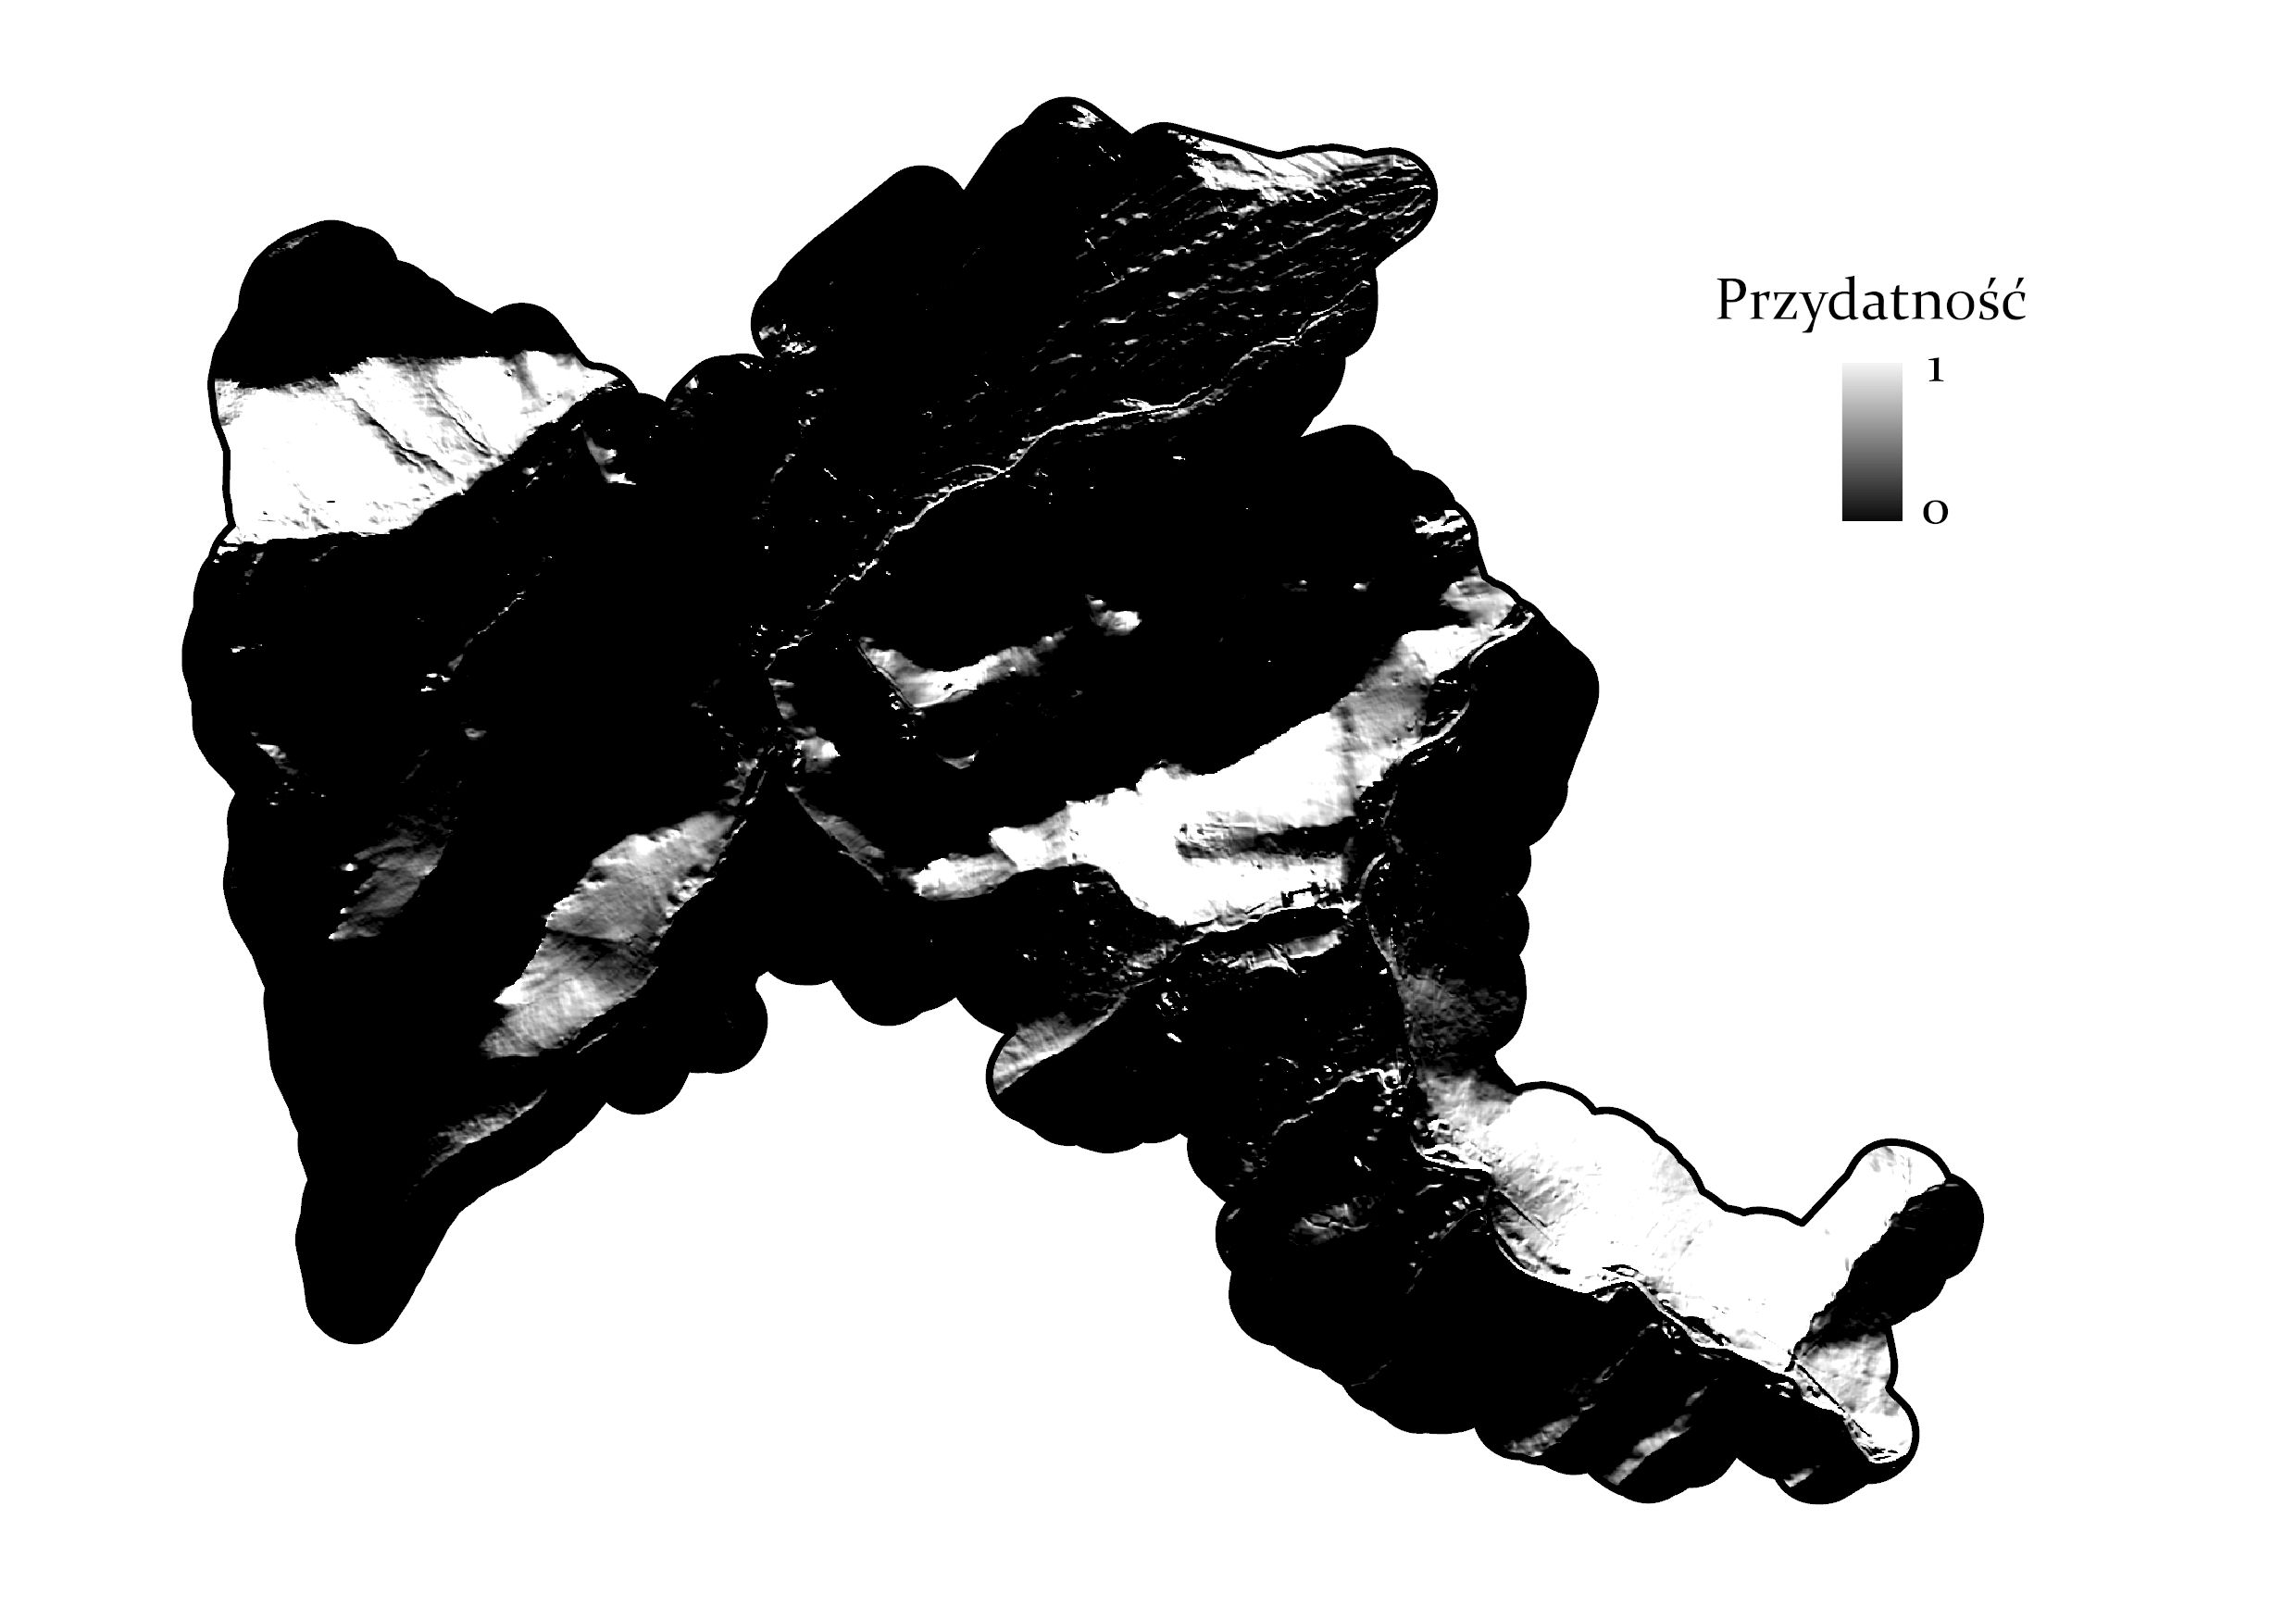
\includegraphics[width=0.75\textwidth]{img/kryterium6-layout.jpg}
    \caption*{Mapa przydatności dla kryterium 6.}
\end{figure}
\vspace{10pt}

Mapę zapisano do geobazy w celu użycia w późniejszym etapie.
\vspace{5pt}

\begin{mintedbox}{python}
aspect_overlay.save(f'{geobaza}\\kryterium_6')
\end{mintedbox}

\newpage
\subsection{Kryterium 7: dojazd do istotnych drogowych węzłów komunikacyjnych}
Warstwę rastrową zawierającą istotne drogowe węzły komunikacyjne utworzono manualnie na podstawie warstwy OT\_SKDR\_L z bazy BDOT10k. Przefiltrowano drogi, pozostawiając jedynie najważniejsze z nich - krajowe, wojewódzkie. Utworzono warstwę punktową, na której umieszczono kilka punktów w miejscach styku tych dróg. Następnie, korzystając z wtyczki \textit{QNEAT3 - QGIS Network Analysis Toolbox 3} oraz dostępnego w niej algorytmu \textit{Iso-Area as Interpolation (from Layer)}. Na podstawie sieci dróg, utworzyła ona raster zawierający dla każdej komórki odległość od węzła komunikacyjnego.

\begin{figure}[H]
    \centering
    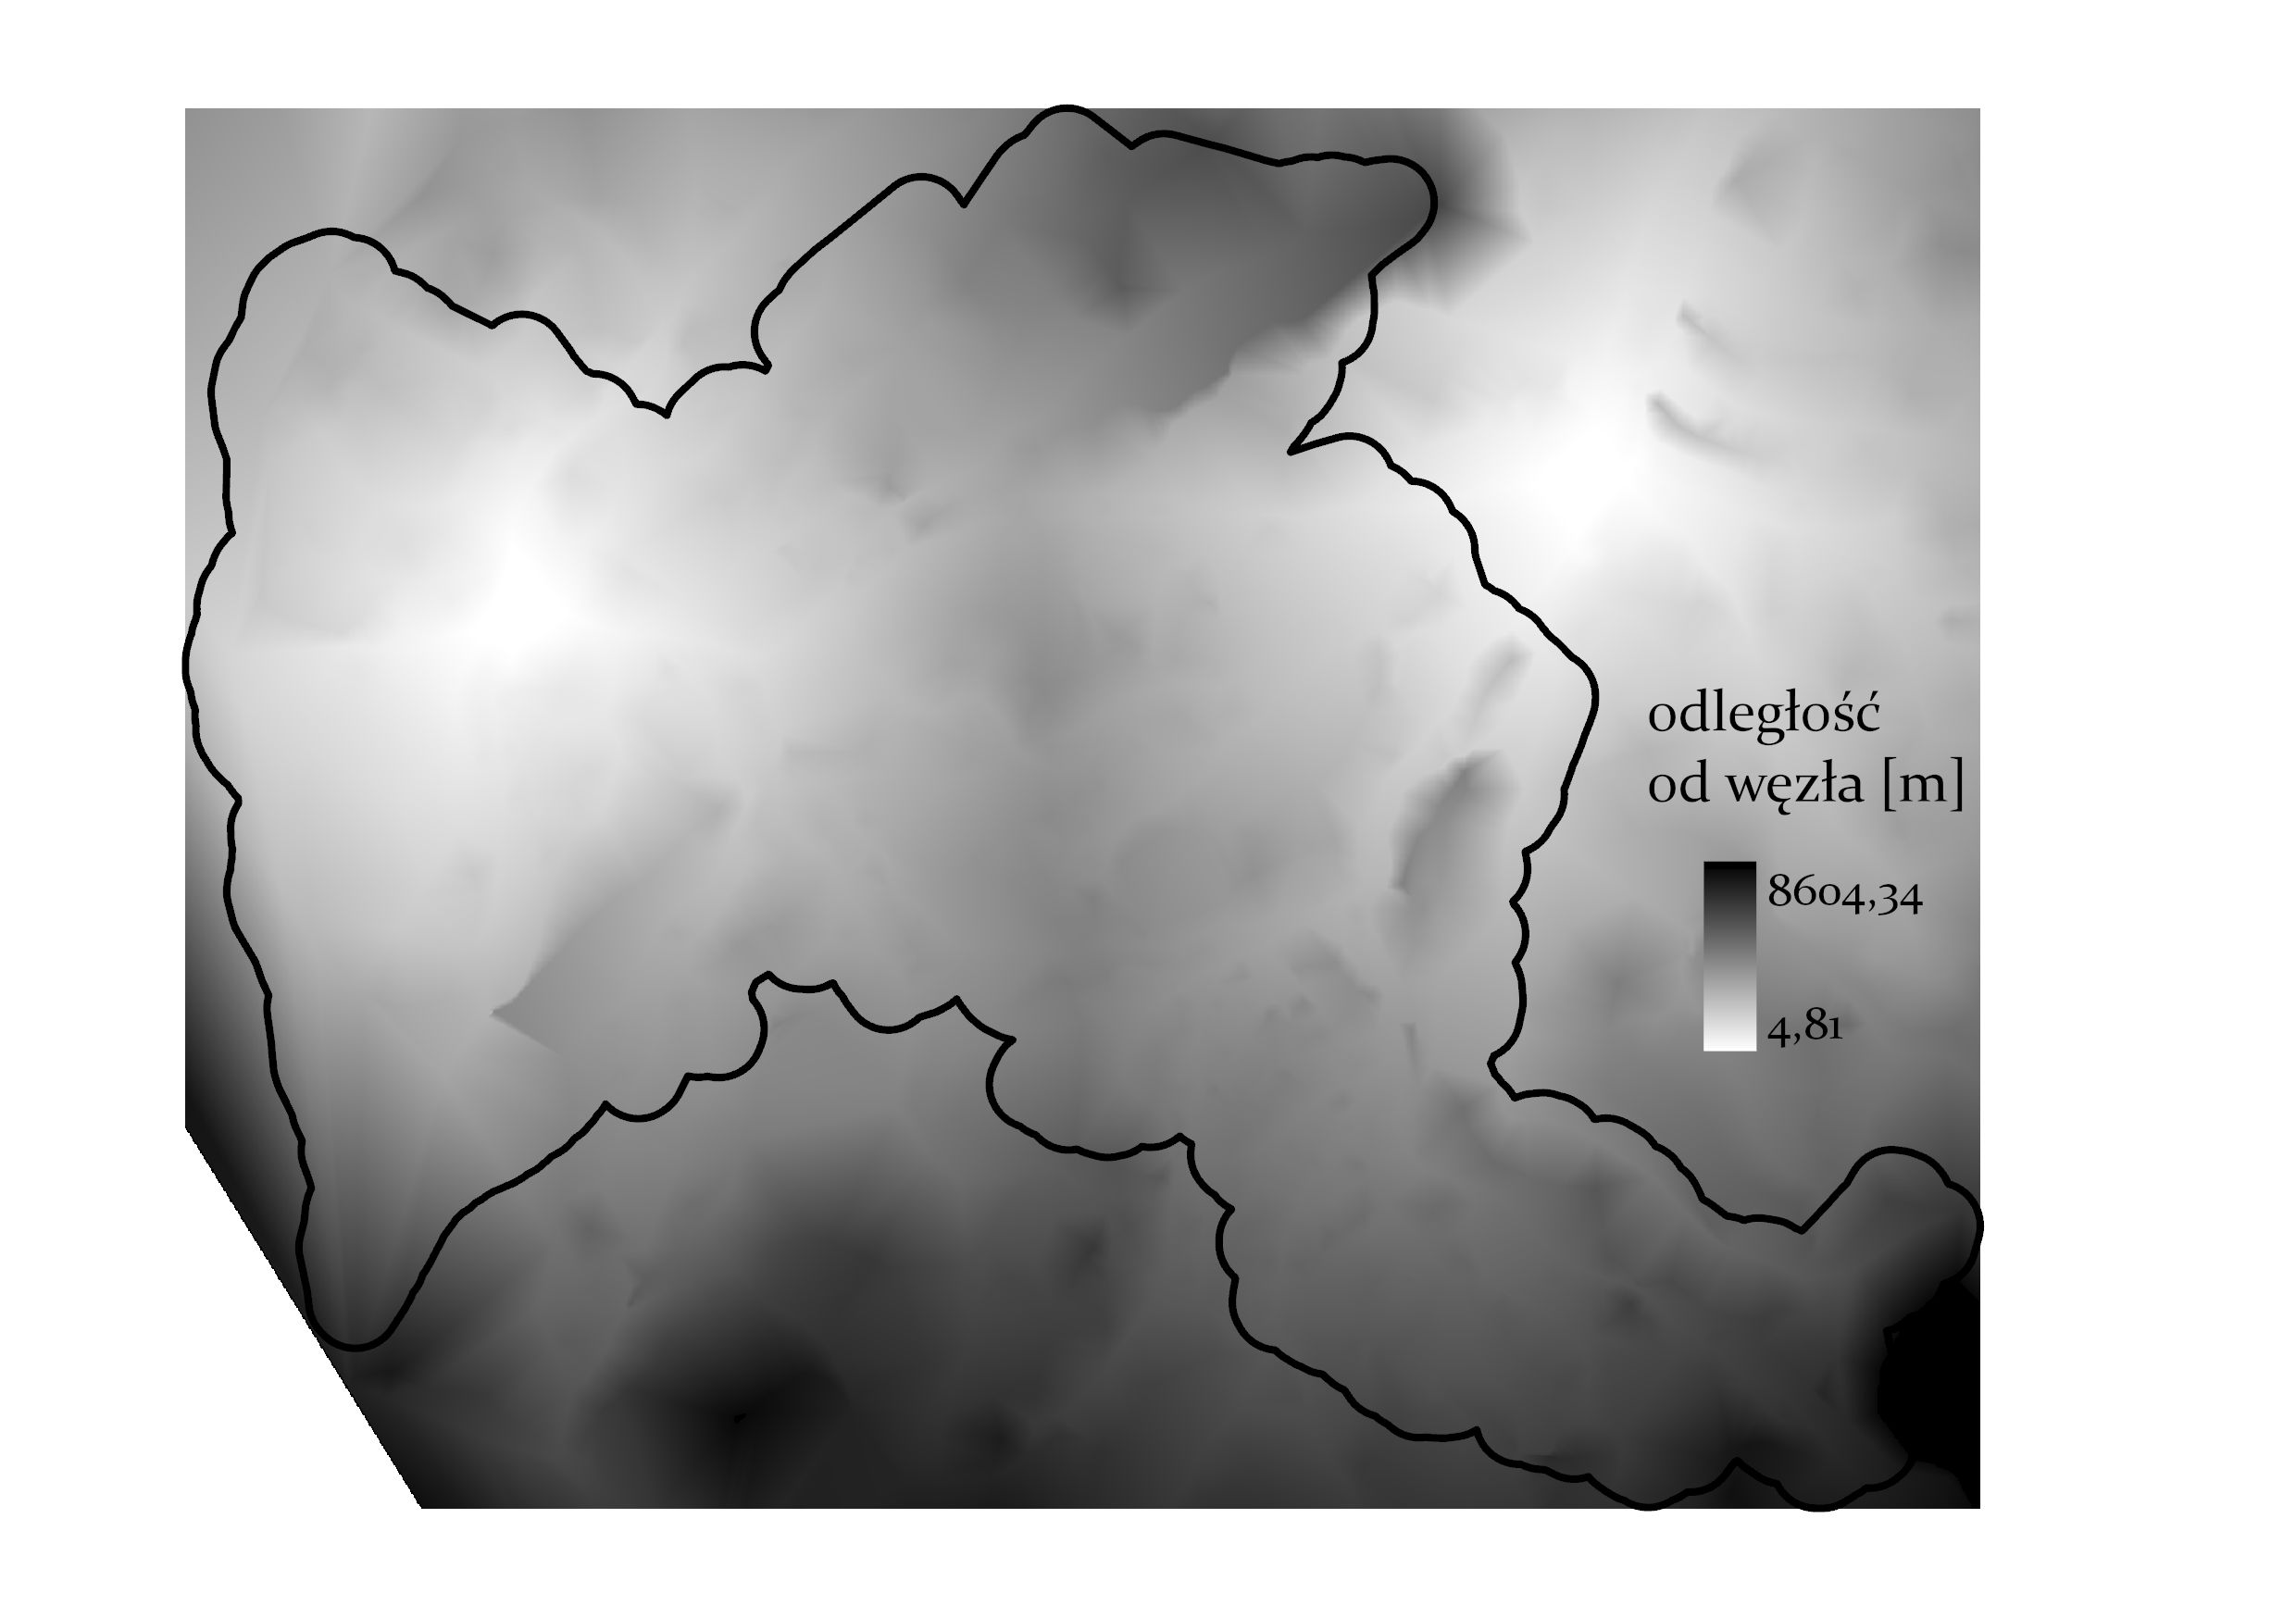
\includegraphics[width=0.75\textwidth]{img/kryterium7-wezly.jpg}
    \caption{Raster utworzony poprzez wtyczkę \textit{QNEAT3}}
\end{figure}
\vspace{10pt}

Dla powyższego rastra obliczono maksymalną odległość od węzła w celu wykorzystania wartości dla funkcji w fuzzy membership.
\vspace{5pt}

\begin{mintedbox}{python}
wezly_max = float(arcpy.management.GetRasterProperties(wezly, "MAXIMUM")[0].replace(',', '.'))
\end{mintedbox}
\vspace{10pt}

Sprawdzono członkostwo na podstawie funkcji liniowej, komórkom od maksymalnej odległości od węzła do połowy maksymalnej odległości od węzła przypisując odpowiednią wartość funkcji, a komórkom położonym bliżej przyporządkowując maksymalną przydatność. 
\vspace{5pt}

\begin{figure}[H]
    \centering
    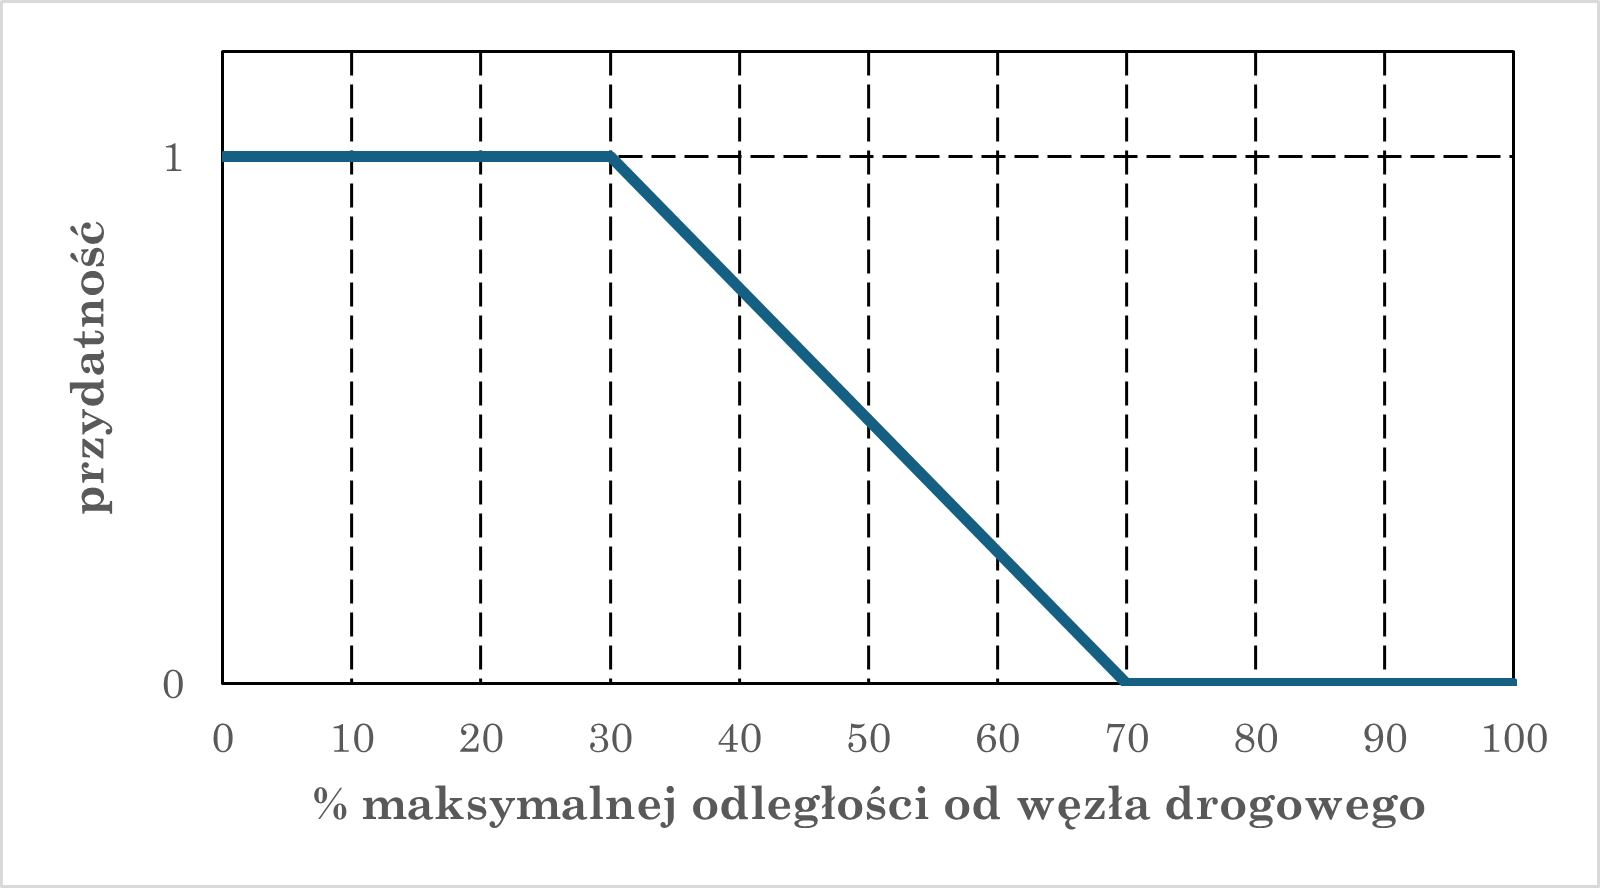
\includegraphics[width=0.6\textwidth]{img/kryterium7-wykres-glowny.png}
    \caption{Reklasyfikacja dla kryterium 7.}
\end{figure}
\vspace{10pt}

Tereny położone w centralnej części rastra okazały się być najbardziej przydatne. Skraje najbardziej na południe oraz północno-wschodnie mają najniższą przydatność.
\vspace{5pt}

\begin{figure}[H]
    \centering
    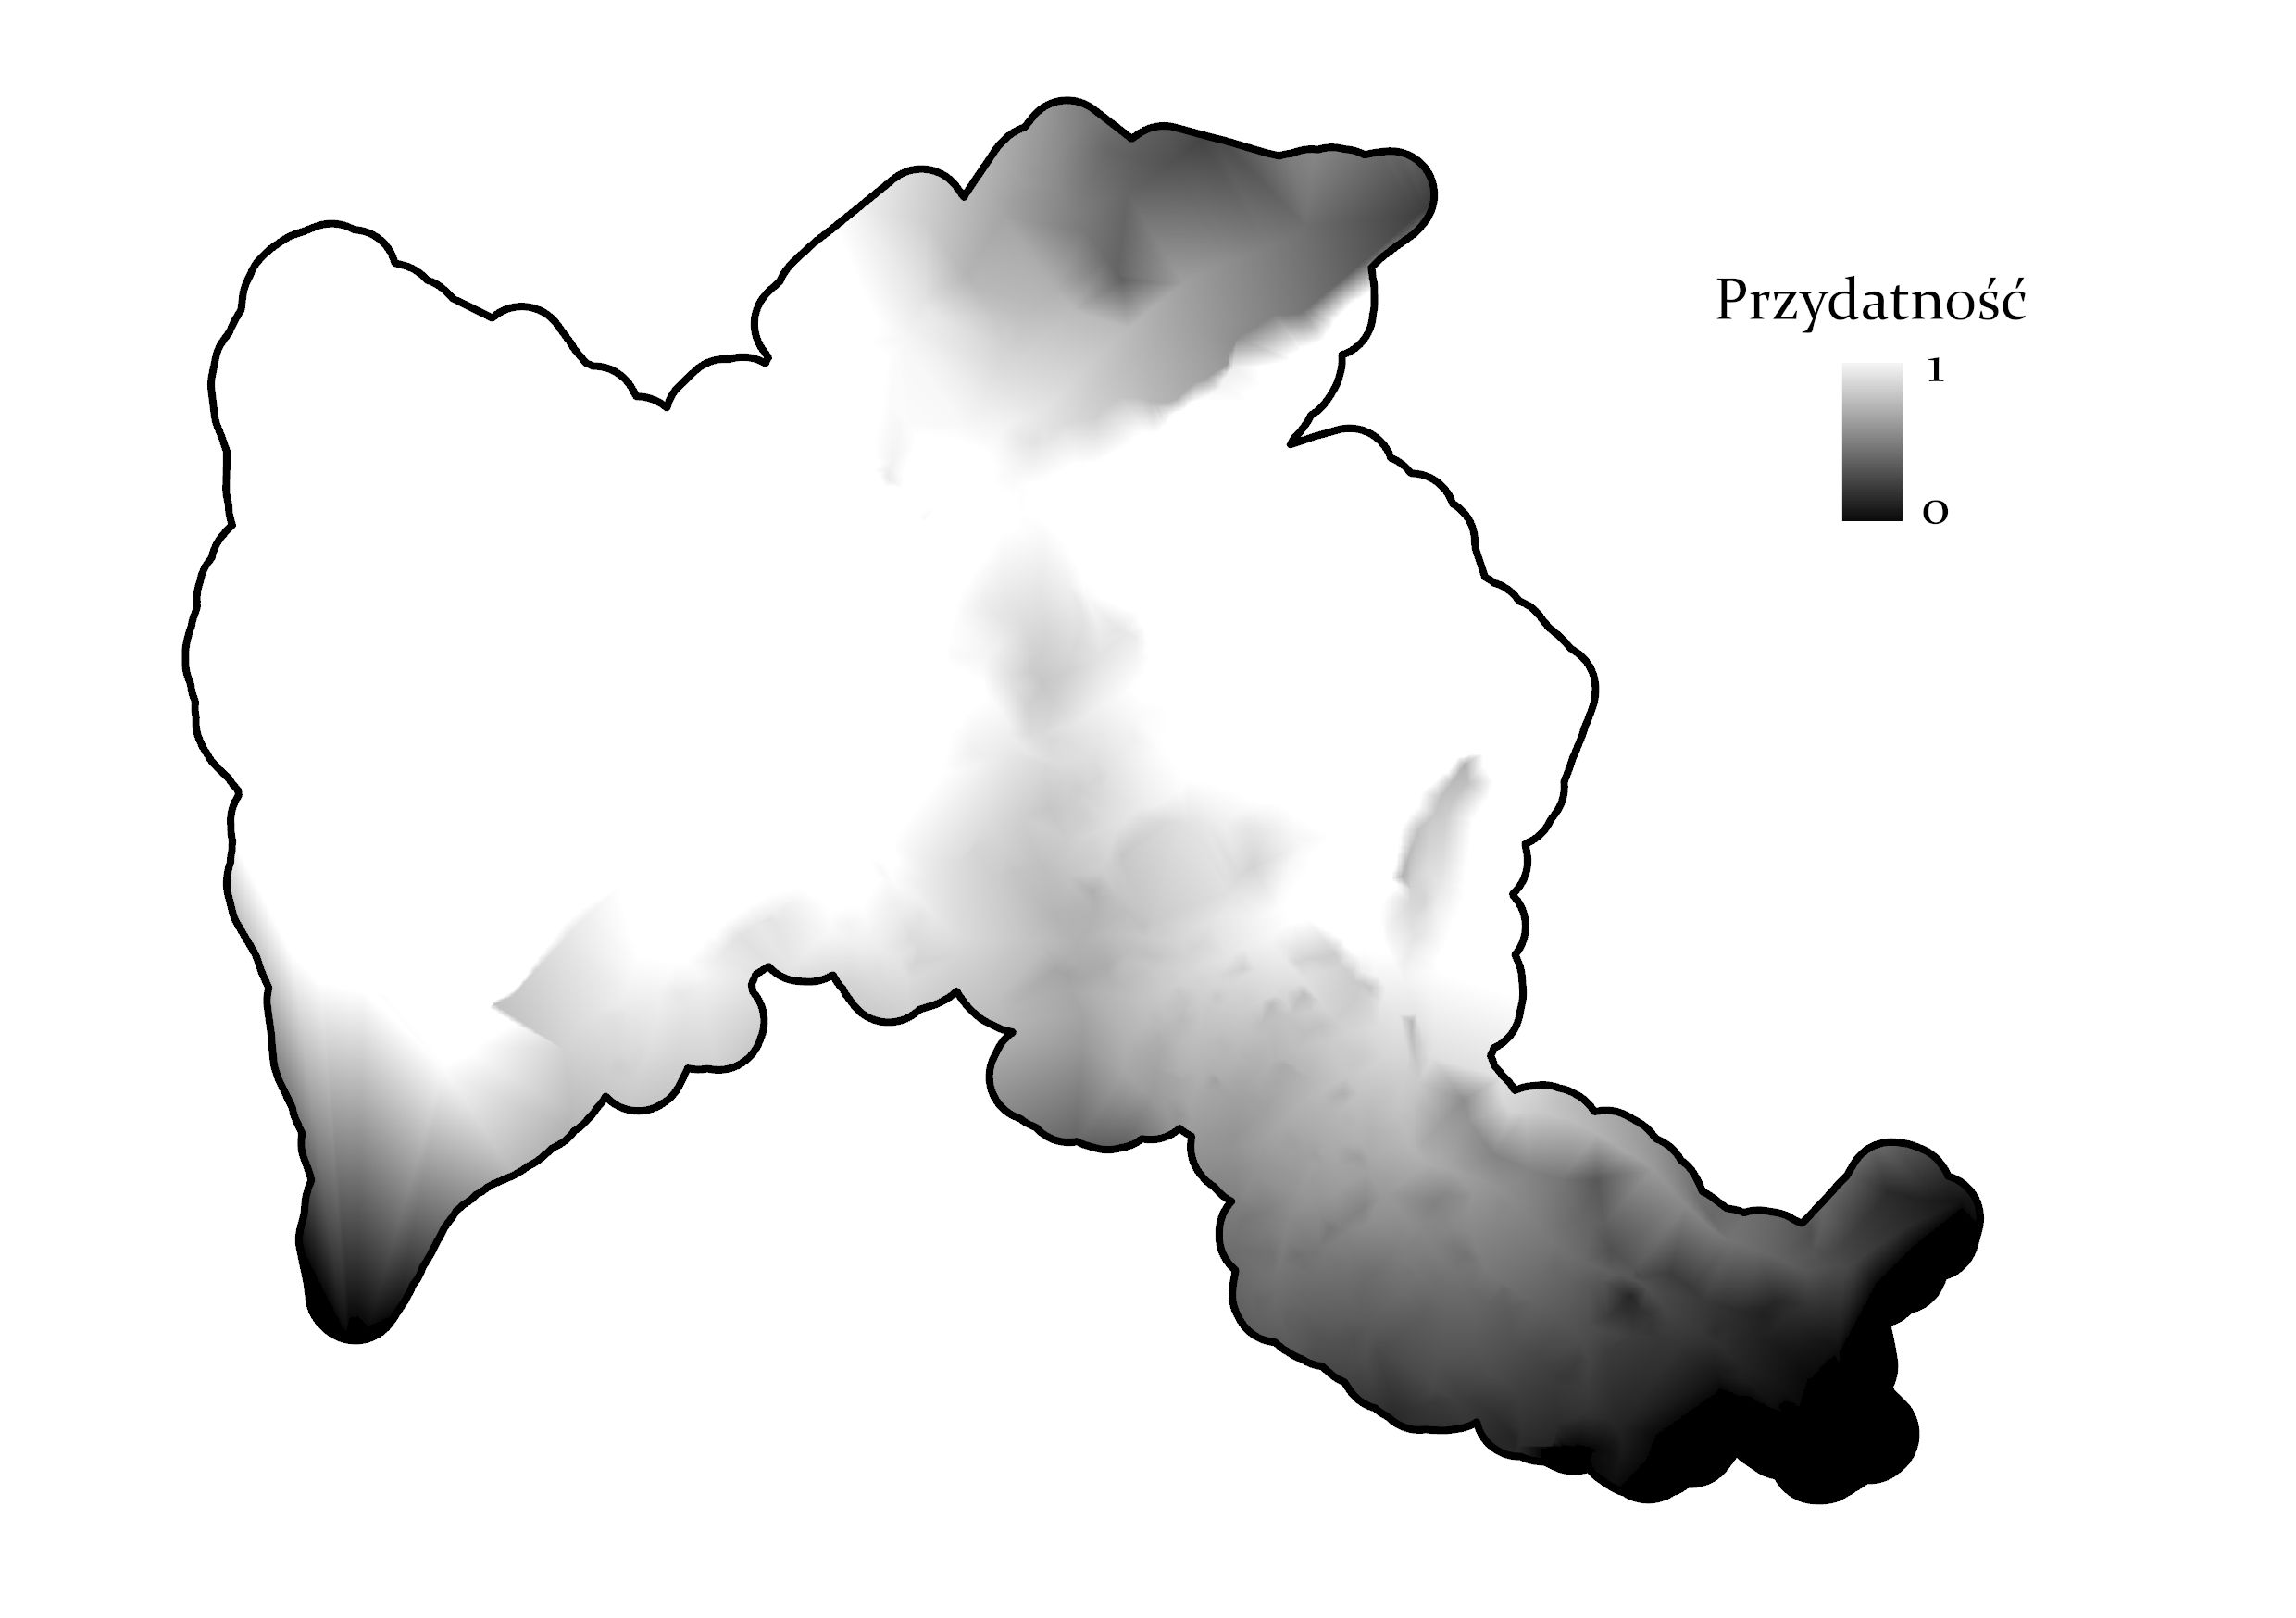
\includegraphics[width=0.75\textwidth]{img/kryterium7-layout.jpg}
    \caption{Mapa przydatności dla kryterium 7.}
\end{figure}
\vspace{10pt}

Mapę zapisano do geobazy w celu użycia w późniejszym etapie.
\vspace{5pt}

\begin{mintedbox}{python}
wezly_fuzzy.save(f'{geobaza}\\kryterium_7')
\end{mintedbox}

\newpage
\subsection{Ocena przydatności terenu}
Poniższy kod najpierw tworzy tabelę zawierającą wagi dla każdego z kryteriów, zmienne w zależności od wariantu. 
\vspace{5pt}

\begin{mintedbox}{python}
tabela_kryteriow = arcpy.sa.WSTable([[f'{geobaza}\\kryterium_1', "VALUE", waga_woda], [f'{geobaza}\\kryterium_2', "VALUE", waga_budynki], [f'{geobaza}\\kryterium_3', "VALUE", waga_lasy], [f'{geobaza}\\kryterium_4', "VALUE", waga_drogi], [f'{geobaza}\\kryterium_5', "VALUE", waga_wysokosc], [f'{geobaza}\\kryterium_6', "VALUE", waga_aspect], [f'{geobaza}\\kryterium_7', "VALUE", waga_wezly]])
\end{mintedbox}
\vspace{10pt}

Następnie tworzy sumę ważoną wszystkich z kryteriów.
\vspace{5pt}

\begin{mintedbox}{python}
weighted_sum = arcpy.sa.WeightedSum(tabela_kryteriow)
weighted_sum.save(f'{geobaza}\\{wariant}_suma_rozmyte')
\end{mintedbox}
\vspace{10pt}

Od teraz do końca sekcji przedstawiane będą podwójne wyniki - pierwszy wynik będzie dla przypadku, gdzie dla każdego kryterium przyjęto tę samą wagę, a drugi dla przypadku, gdzie wagi są różne. Poniżej przedstawiono przyjęte wagi w obu podejściach.
\begin{table}[ht]
    \begin{minipage}{0.48\textwidth}
        \centering
        \renewcommand{\arraystretch}{1.2}
        \begin{tabular}{|p{4cm}|p{1.4cm}|}
        \hline
        \textbf{Kryterium} & \textbf{Waga}\\
        \hline
        1 (odległość od rzek i zbiorników wodnych) & 0.142857\\
        \hline
        2 (odległość od budynków mieszkalnych) & 0.142857\\
        \hline
        3 (pokrycie terenu) & 0.142857\\
        \hline
        4 (dostęp do dróg utwardzonych) & 0.142857\\
        \hline
        5 (nachylenie stoków) & 0.142857\\    
        \hline
        6 (dostęp światła słonecznego) & 0.142857\\
        \hline
        7 (dobry dojazd do istotnych węzłów komunikacyjnych) & 0.142857\\
        \hline
        \end{tabular}
        \caption{Tabela z równymi wagami dla kryteriów}
        \label{tab:bdot_costs_equal}
    \end{minipage}
    \hfill
    \begin{minipage}{0.48\textwidth}
        \centering
        \renewcommand{\arraystretch}{1.2}
        \begin{tabular}{|p{4cm}|p{1cm}|}
        \hline
        \textbf{Kryterium} & \textbf{Waga}\\
        \hline
        1 (odległość od rzek i zbiorników wodnych) & 0.10\\
        \hline
        2 (odległość od budynków mieszkalnych) & 0.15\\
        \hline
        3 (pokrycie terenu) & 0.20\\
        \hline
        4 (dostęp do dróg utwardzonych) & 0.10\\
        \hline
        5 (nachylenie stoków) & 0.15\\    
        \hline
        6 (dostęp światła słonecznego) & 0.25\\
        \hline
        7 (dobry dojazd do istotnych węzłów komunikacyjnych) & 0.05\\
        \hline
        \end{tabular}
        \caption{Tabela z różnymi wagami dla kryteriów}
        \label{tab:bdot_costs_different}
    \end{minipage}
\end{table}


\begin{figure}[H]
    \begin{minipage}[t]{0.48\textwidth}
        \centering
        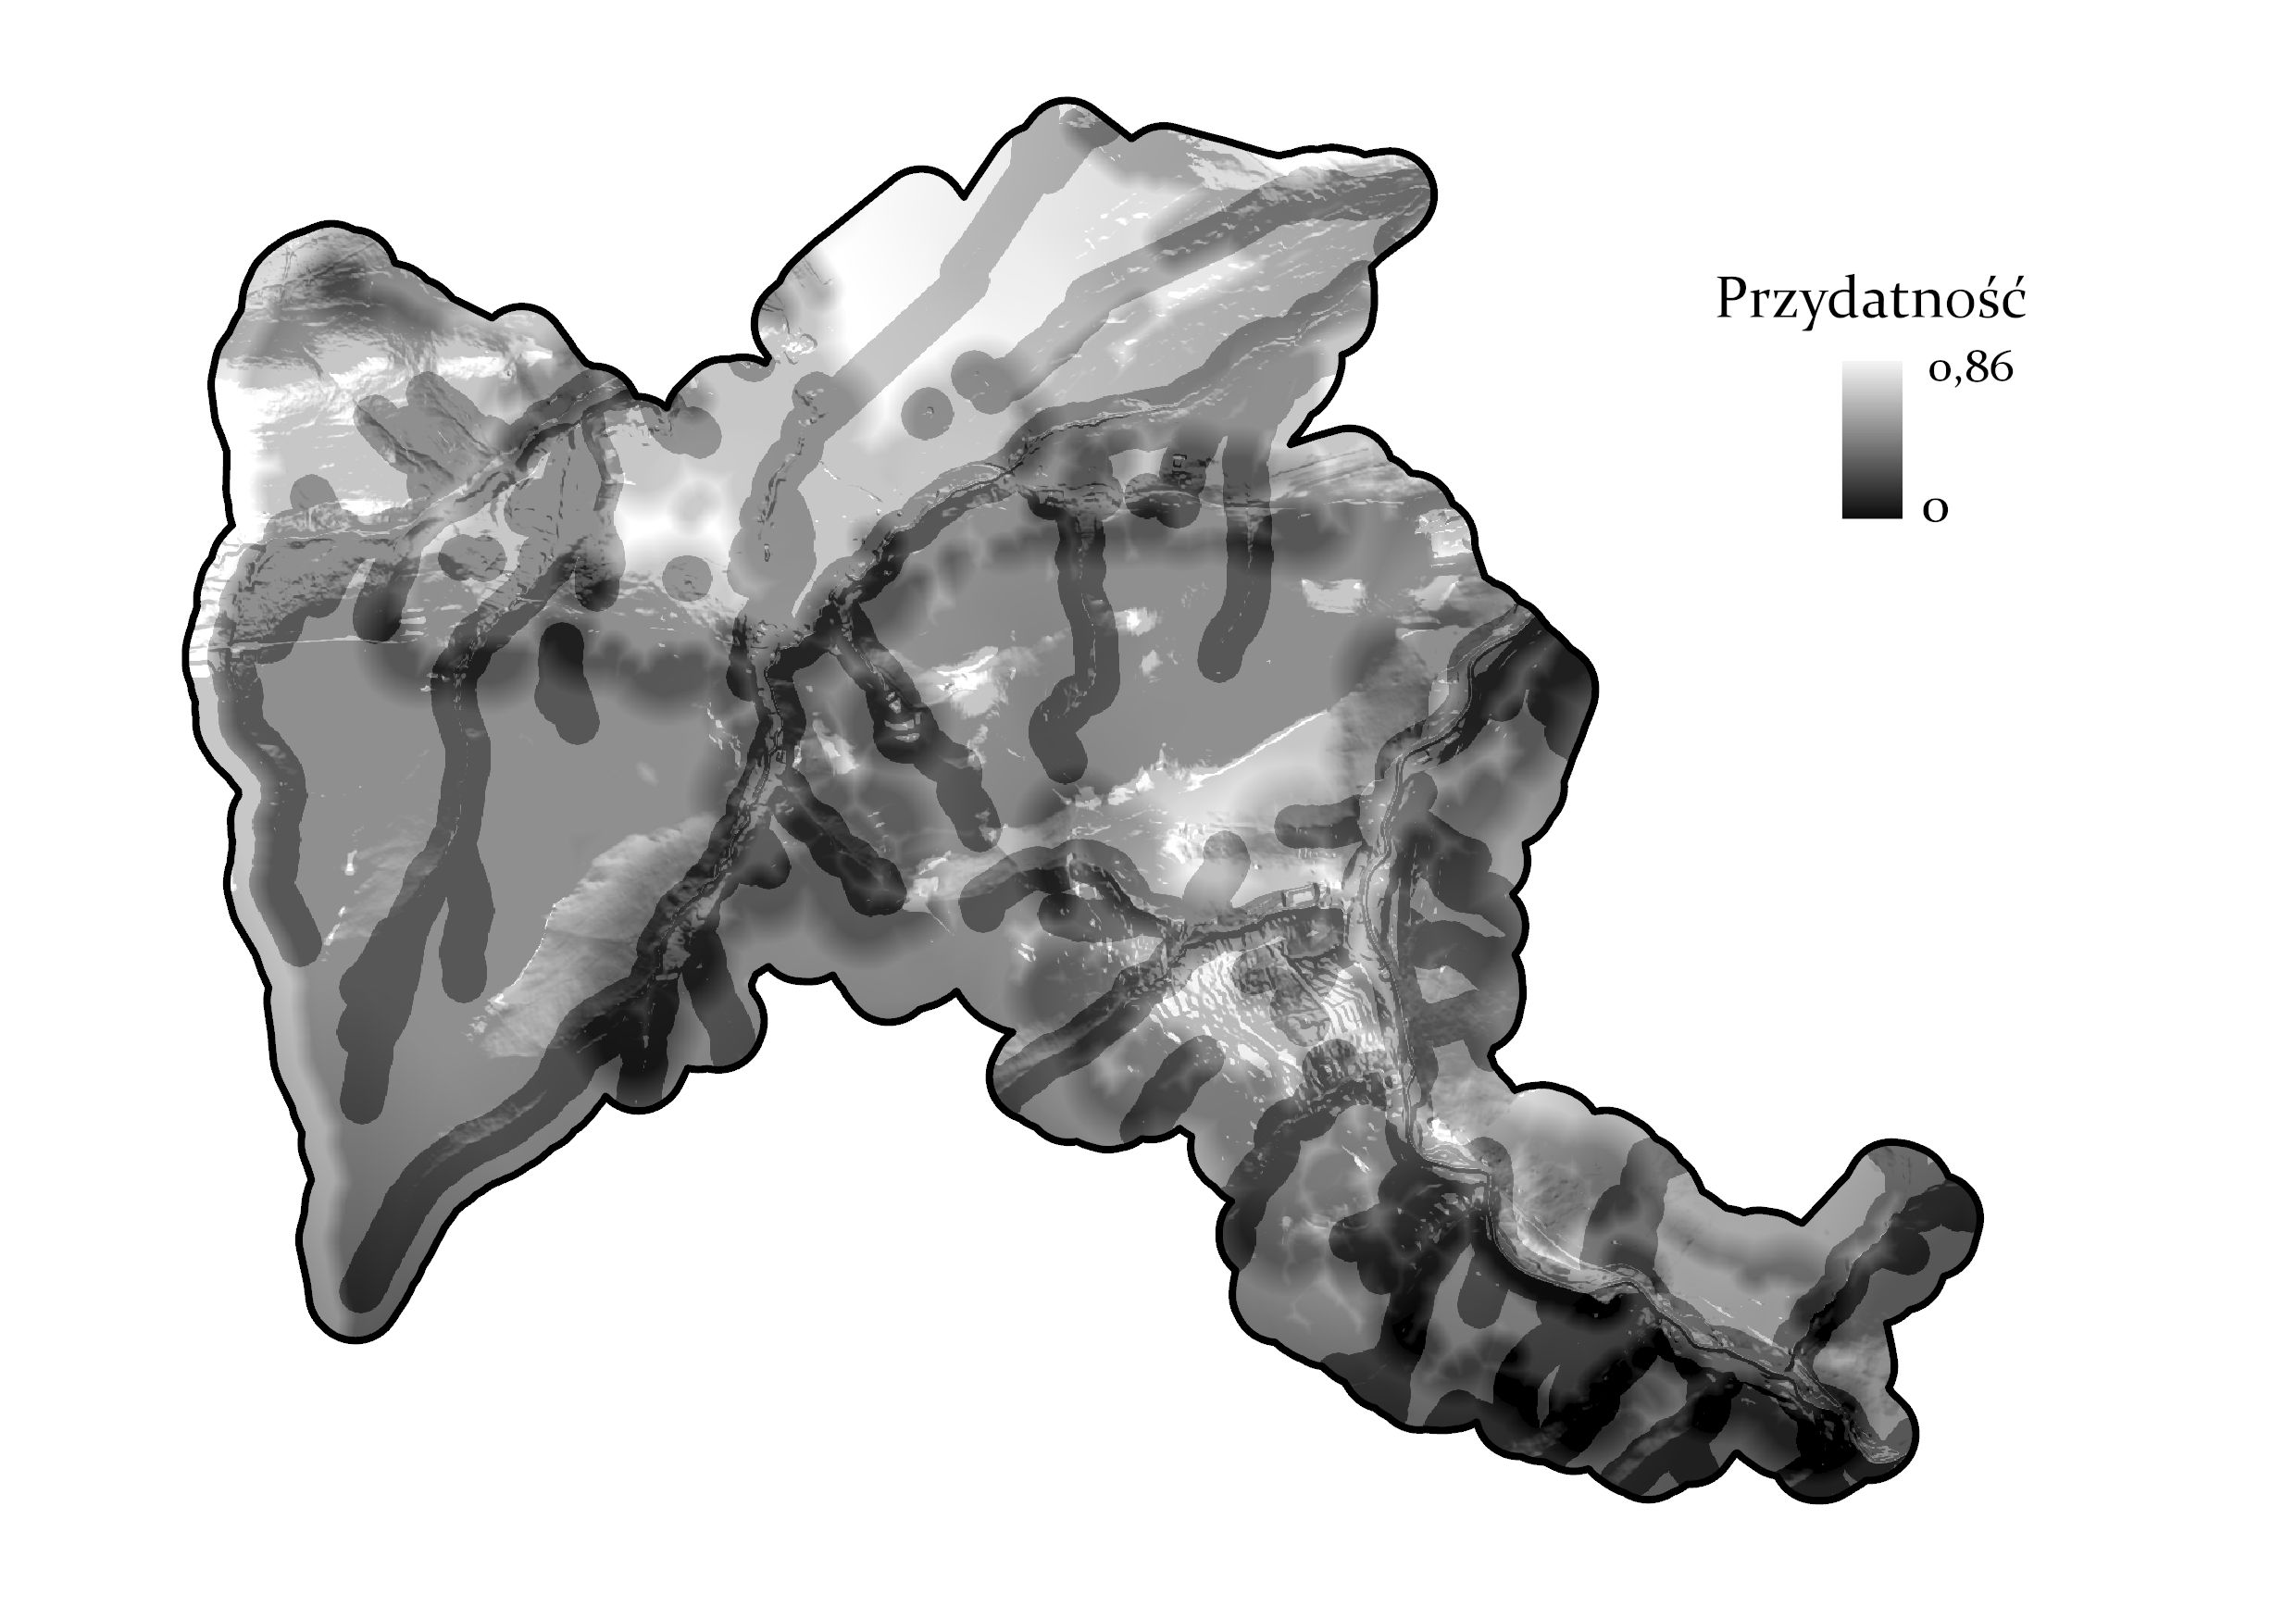
\includegraphics[width=\linewidth]{img/rozmyte-layout.jpg}
        \caption{Suma kryteriów rozmytych - wagi równe}
        \label{fig:rozmyte-rowne}
    \end{minipage}
    \hfill
    \begin{minipage}[t]{0.48\textwidth}
        \centering
        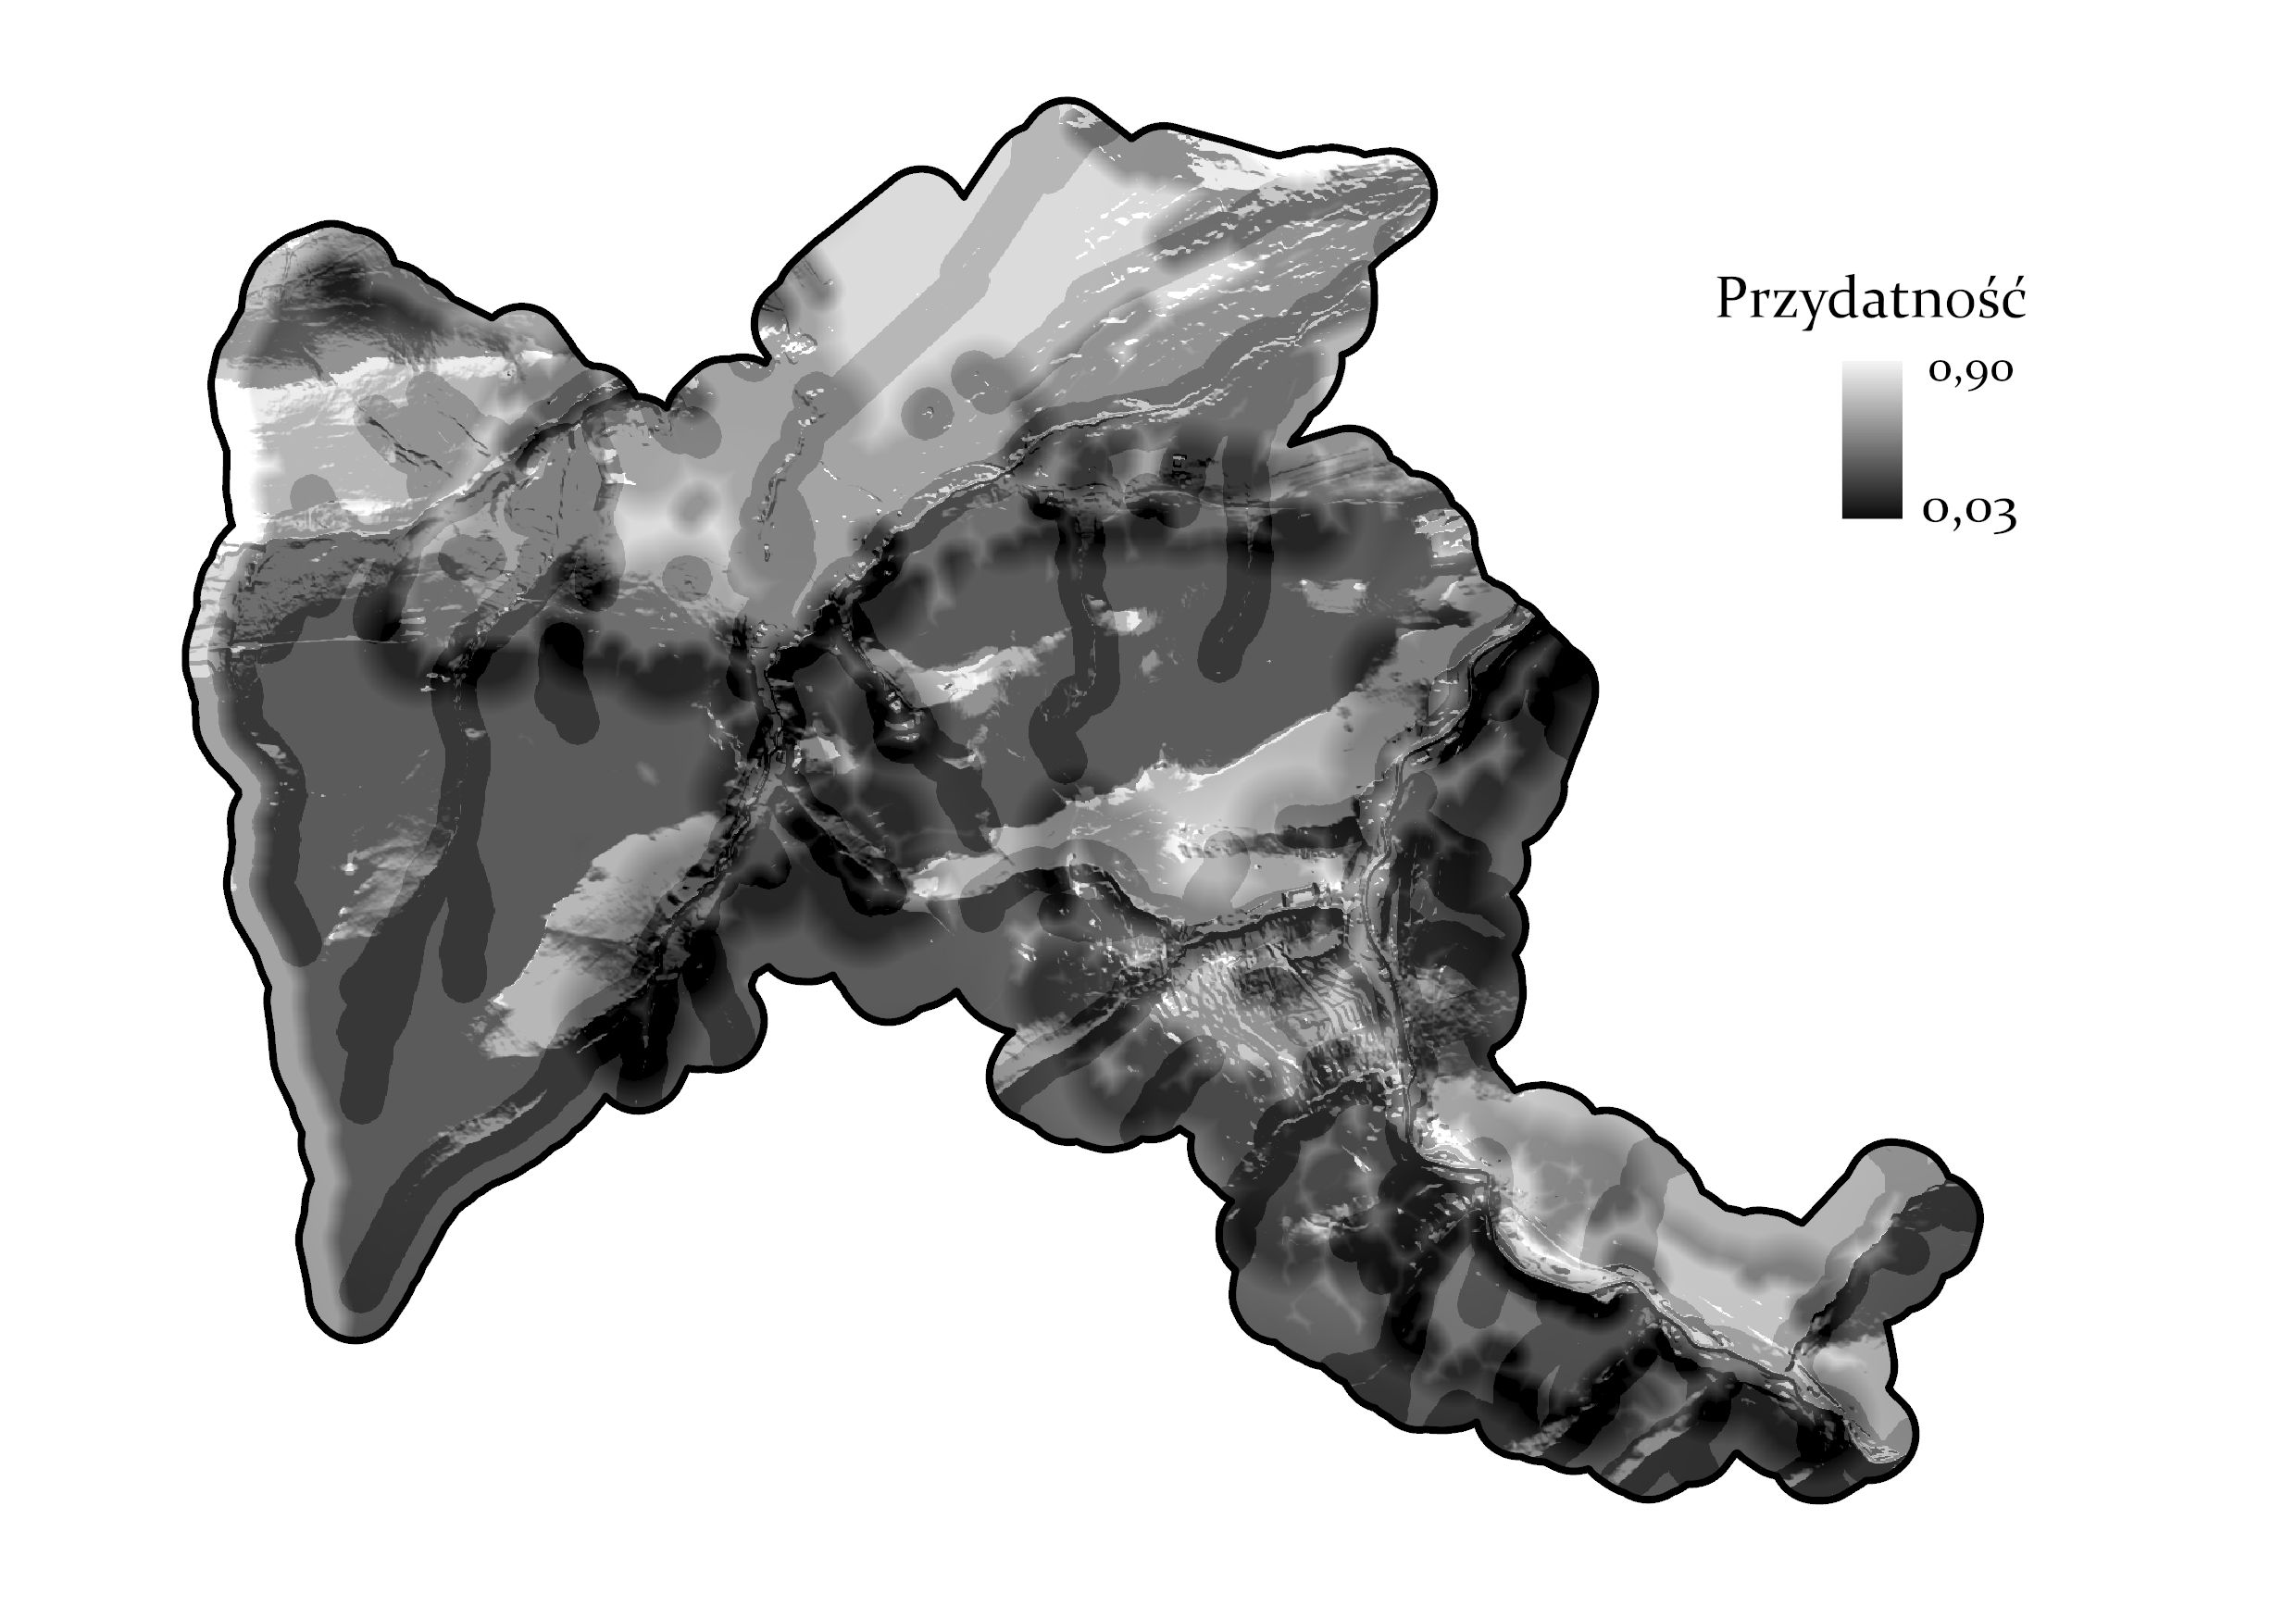
\includegraphics[width=\linewidth]{img/roznewagi-rozmyte-layout.jpg}
        \caption{Suma kryteriów rozmytych - wagi różne}
        \label{fig:rozmyte-rozne}
    \end{minipage}
\end{figure}

\vspace{5pt}

Później brane są pod uwagę kryteria ostre, tj. 100-metrowa strefa ochronna od wód, 150-metrowa odległość od budynków mieszkalnych oraz 15-metrowa odległość od lasów. W funkcji \textit{FuzzyOverlay} wybrano parametr \textit{AND}, dzięki czemu zostaje utworzony raster, który przyjmuje najniższą możliwą wartość dla komórki. 
\vspace{5pt}

\begin{mintedbox}{python}
kryteria_ostre = arcpy.sa.FuzzyOverlay([woda_rosnaca, f"{geobaza}\\kryterium_2", f"{geobaza}\\kryterium_3"], 'AND')
kryteria_ostre.save(f'{geobaza}\\kryteria_ostre')
\end{mintedbox}
\vspace{10pt}

\begin{figure}[H]
    \centering
    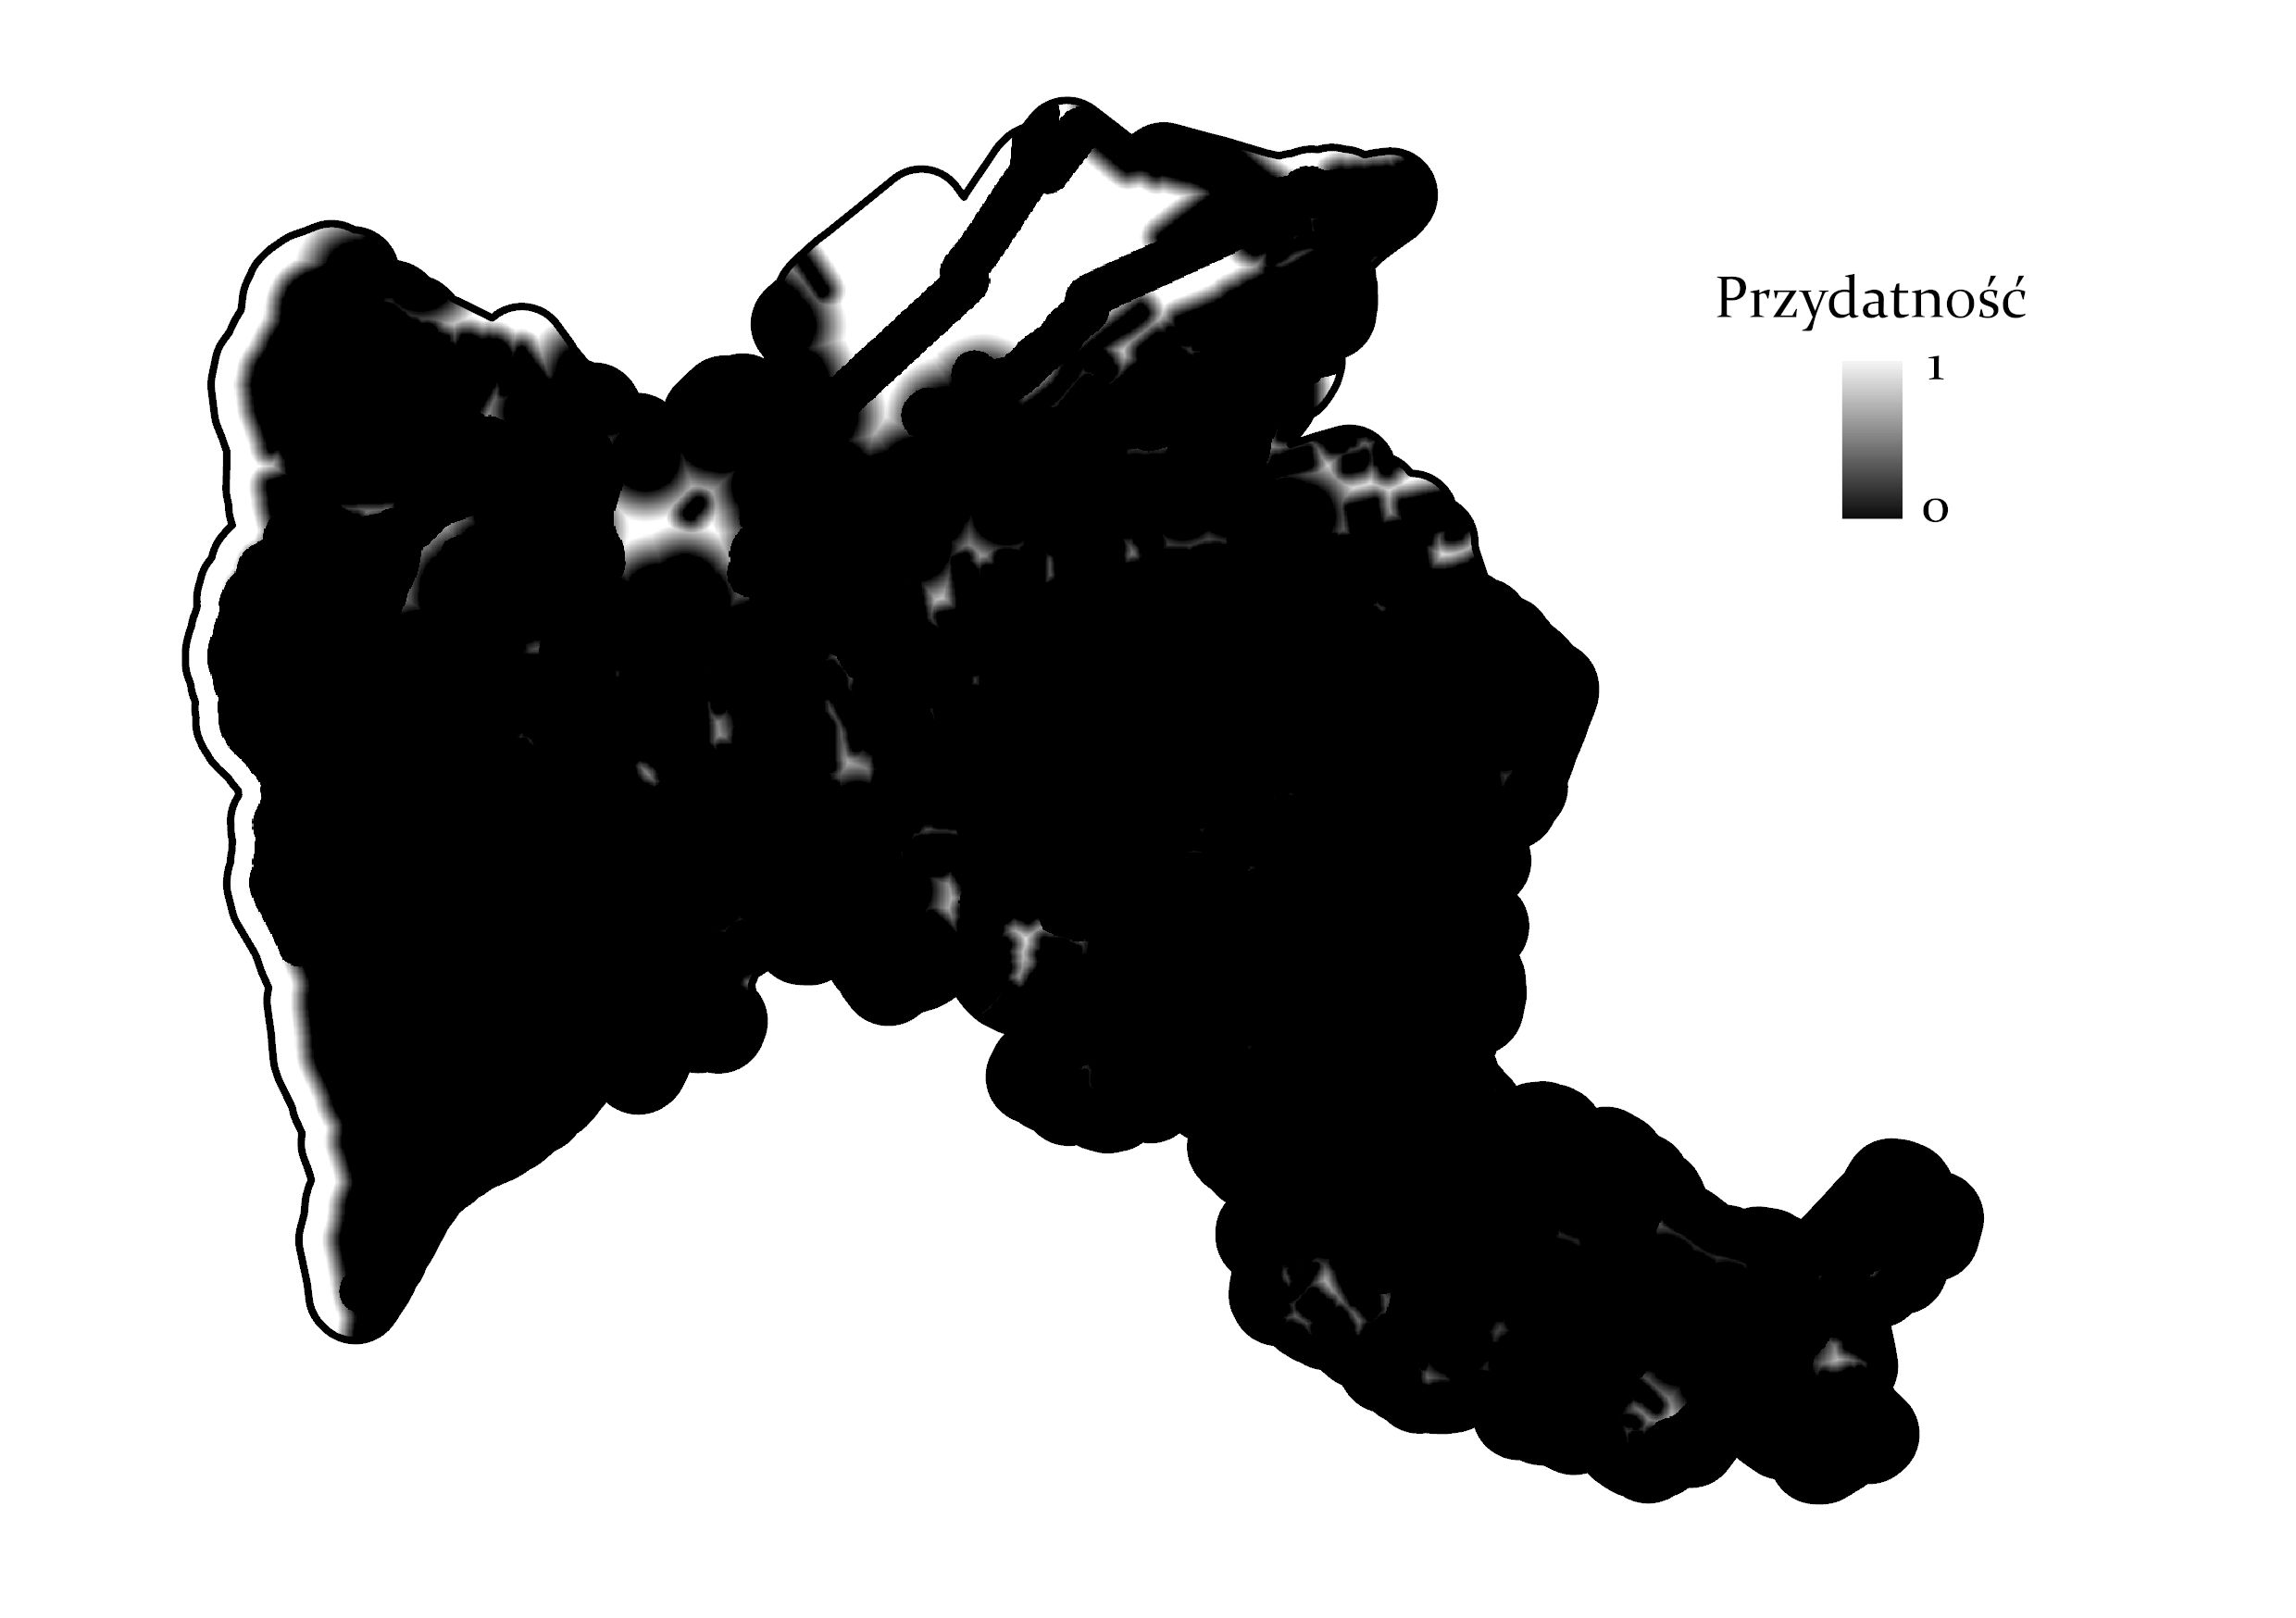
\includegraphics[width=0.65\textwidth]{img/ostre-layout.jpg}
    \caption{Suma kryteriów ostrych}
\end{figure}
\vspace{10pt}

Następnie zostaje utworzony iloczyn kryteriów ostrych i rozmytych. W ten sposób eliminowane z dalszych analiz są komórki wykluczone przez któreś z kryteriów ostrych.
\vspace{5pt}

\begin{mintedbox}{python}
iloczyn = arcpy.sa.FuzzyOverlay([kryteria_ostre, weighted_sum], 'AND')
iloczyn.save(f'{geobaza}\\{wariant}_wynik')
\end{mintedbox}
\vspace{10pt}

\begin{figure}[H]
    \begin{minipage}[t]{0.48\textwidth}
        \centering
        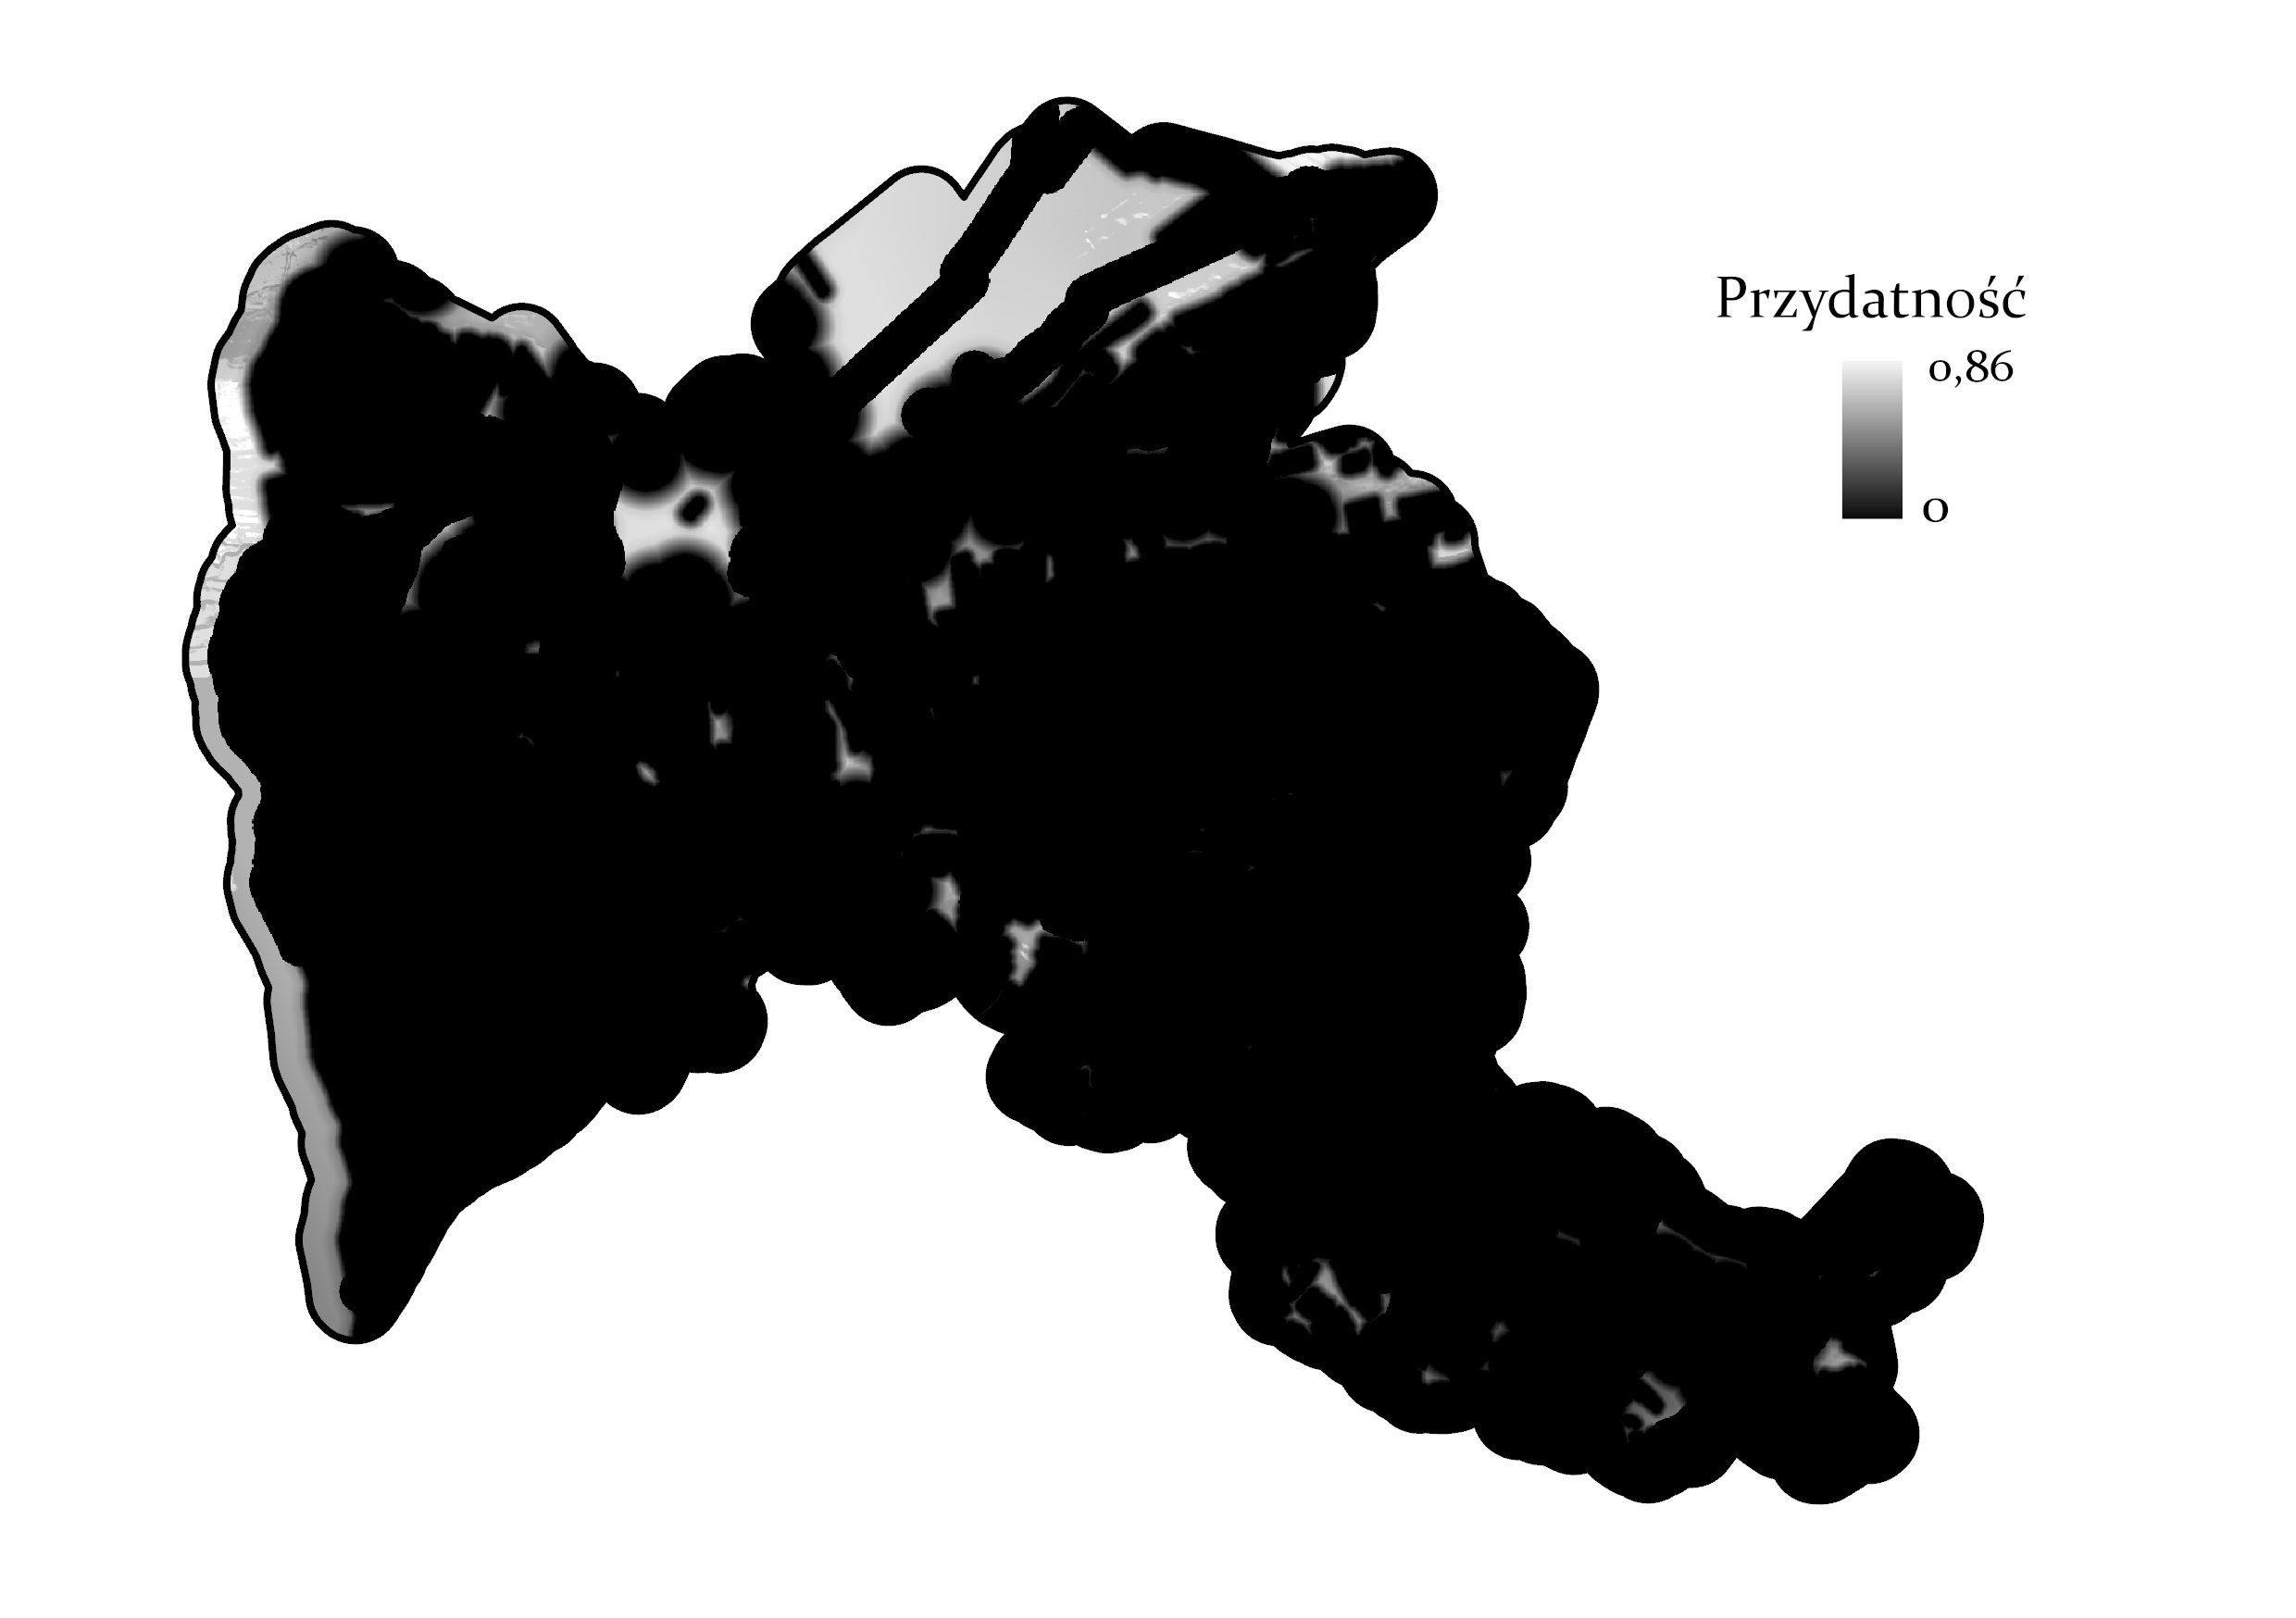
\includegraphics[width=\linewidth]{img/wynik.jpg}
        \caption{Wynik łączenia kryteriów ostrych i rozmytych - wagi równe}
        \label{fig:wynik-rowne}
    \end{minipage}
    \hfill
    \begin{minipage}[t]{0.48\textwidth}
        \centering
        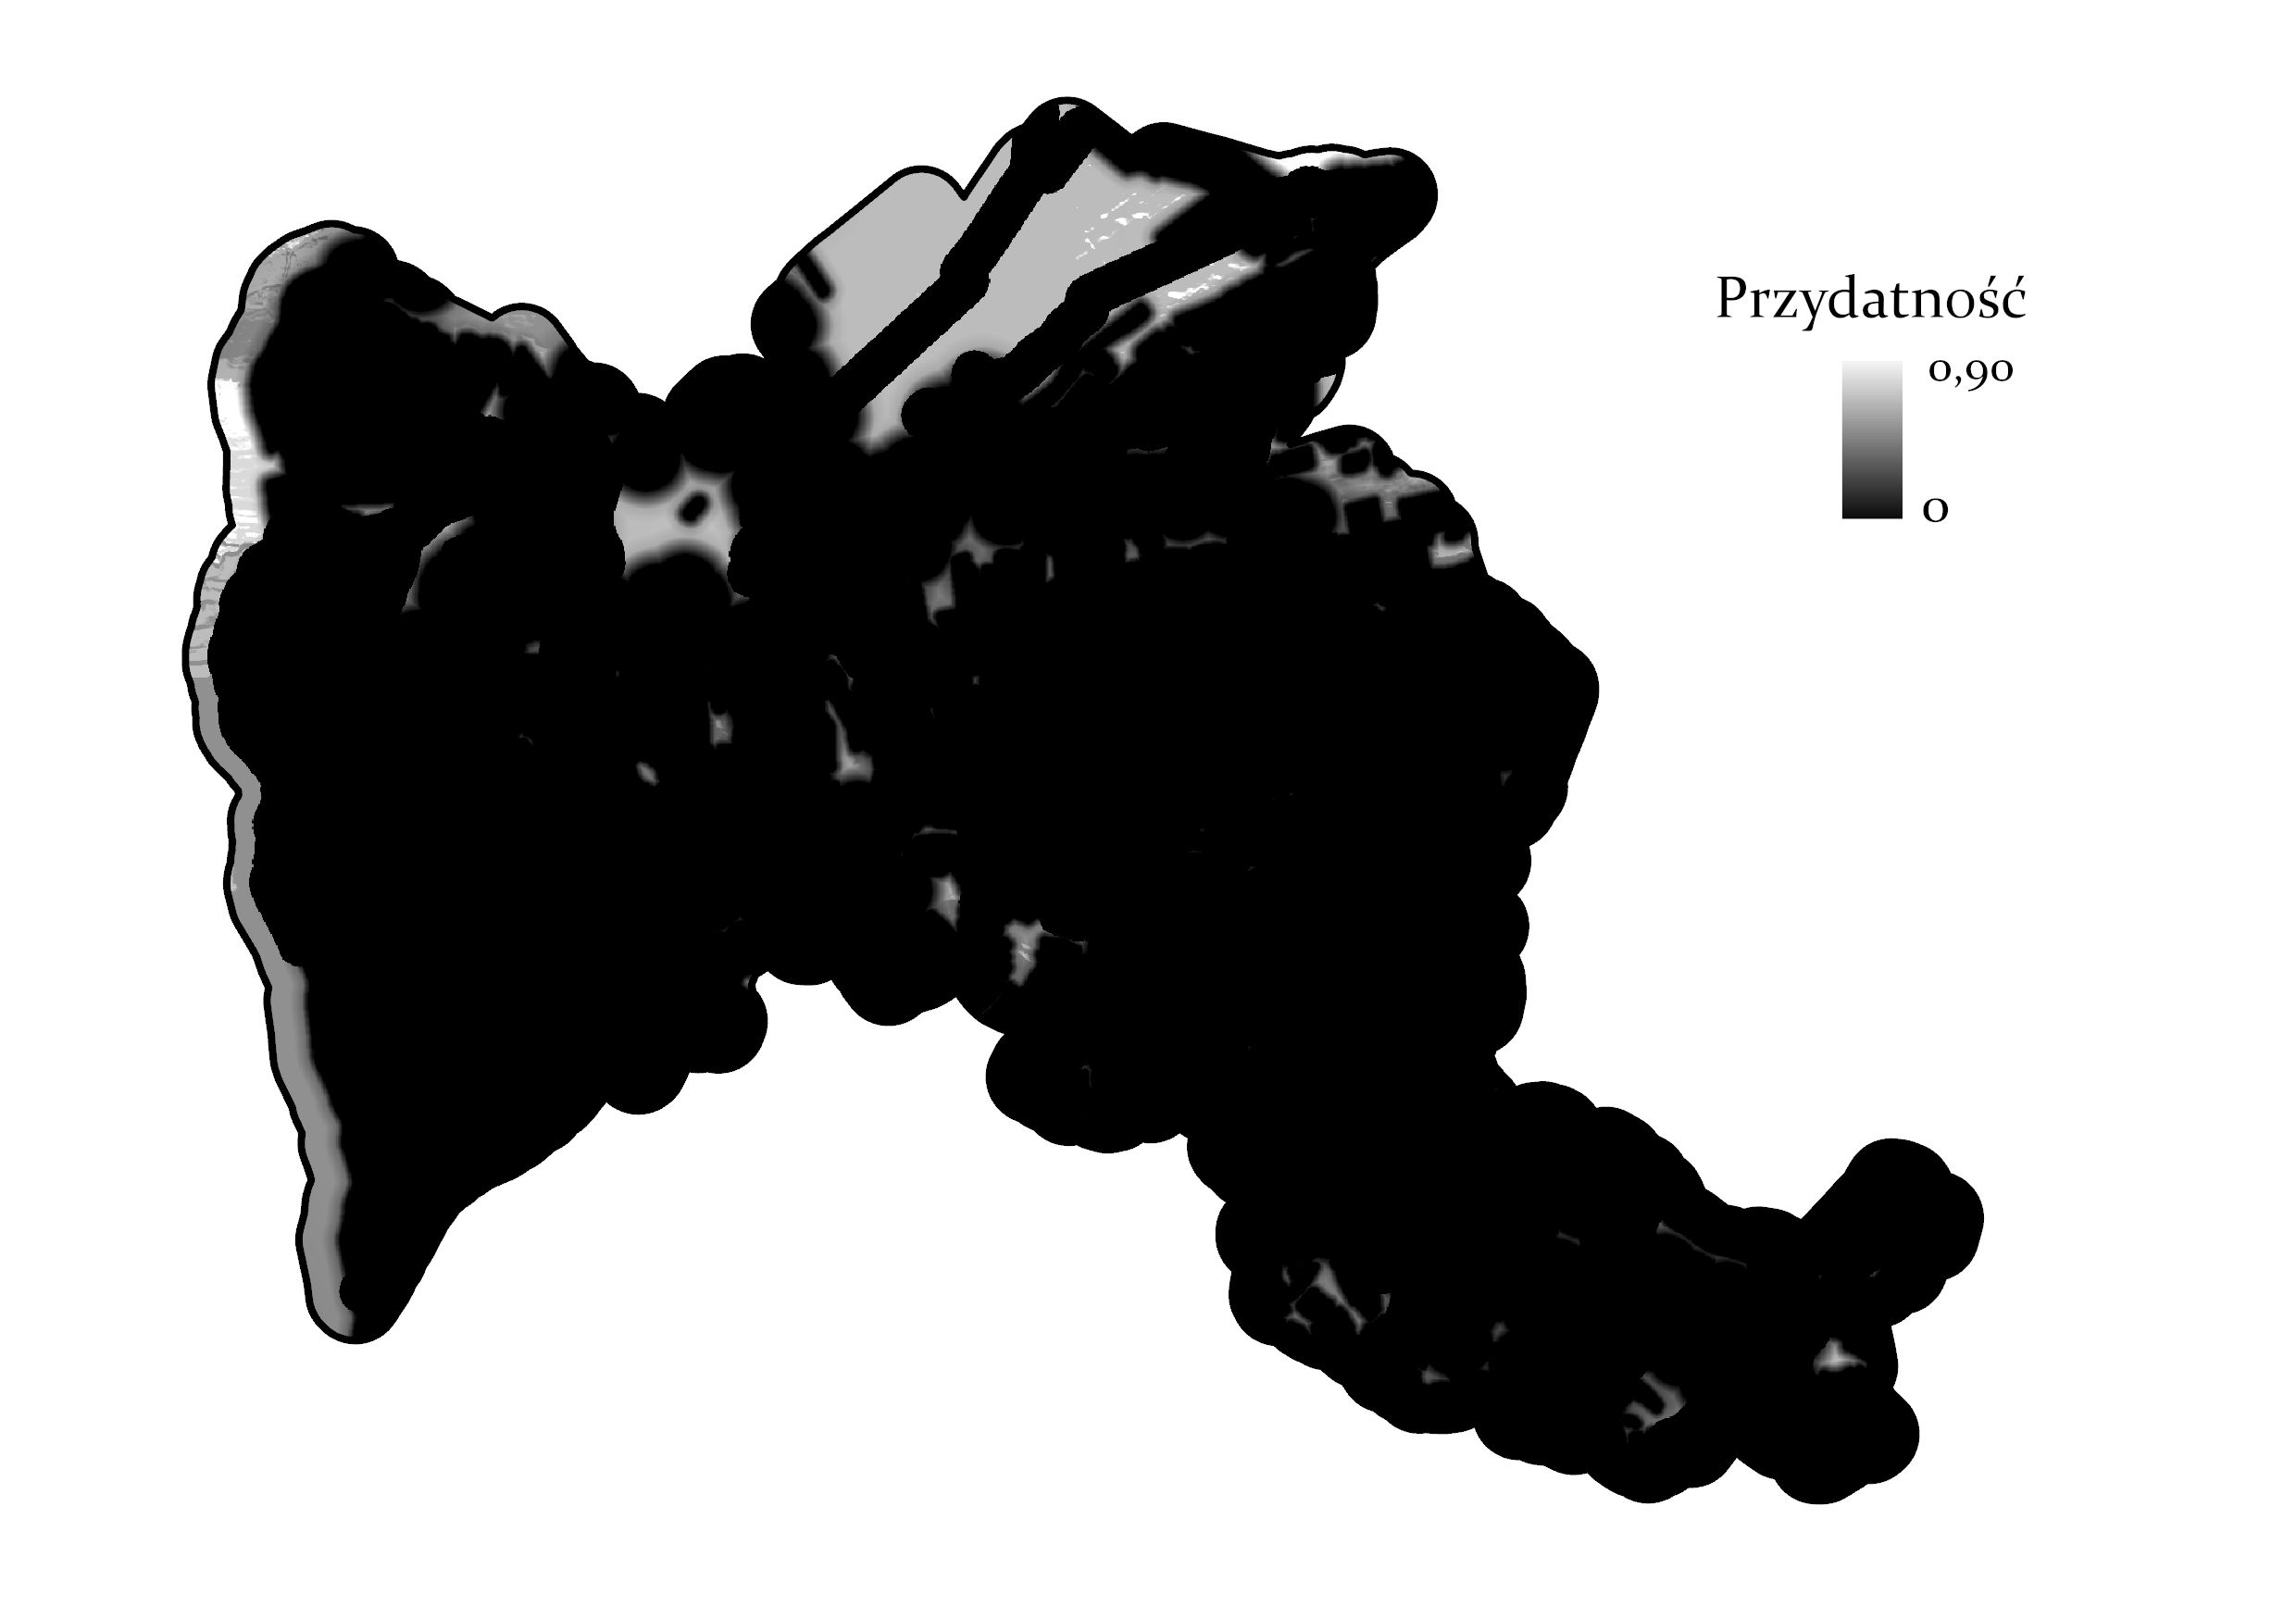
\includegraphics[width=\linewidth]{img/roznewagi-wynik.jpg}
        \caption{Wynik łączenia kryteriów ostrych i rozmytych - wagi różne}
        \label{fig:wynik-rozne}
    \end{minipage}
\end{figure}

\vspace{10pt}

Przed reklasyfikacją, obliczana jest maksymalna przydatność na obszarze.
\vspace{5pt}

\begin{mintedbox}{python}
arcpy.management.CalculateStatistics(iloczyn)
max_przydatnosc = iloczyn.maximum
\end{mintedbox}
\vspace{10pt}

Utworzony przez połączenie kryteriów ostrych i rozmytych raster reklasyfikujemy, przyporządkowując komórkom o przydatności powyżej określonego progu przydatności wartość 1, a pozostałym komórkom - wartość 0.
\vspace{5pt}

\begin{mintedbox}{python}
wynik_reclassified = arcpy.sa.Reclassify(iloczyn, "VALUE", arcpy.sa.RemapRange([[0, prog_przydatnosci * max_przydatnosc, 0], [prog_przydatnosci * max_przydatnosc, 1, 1]]))
wynik_reclassified.save(f'{geobaza}\\{wariant}_wynik_reclassified')
\end{mintedbox}
\vspace{5pt}

\begin{figure}[H]
    \begin{minipage}[t]{0.48\textwidth}
        \centering
        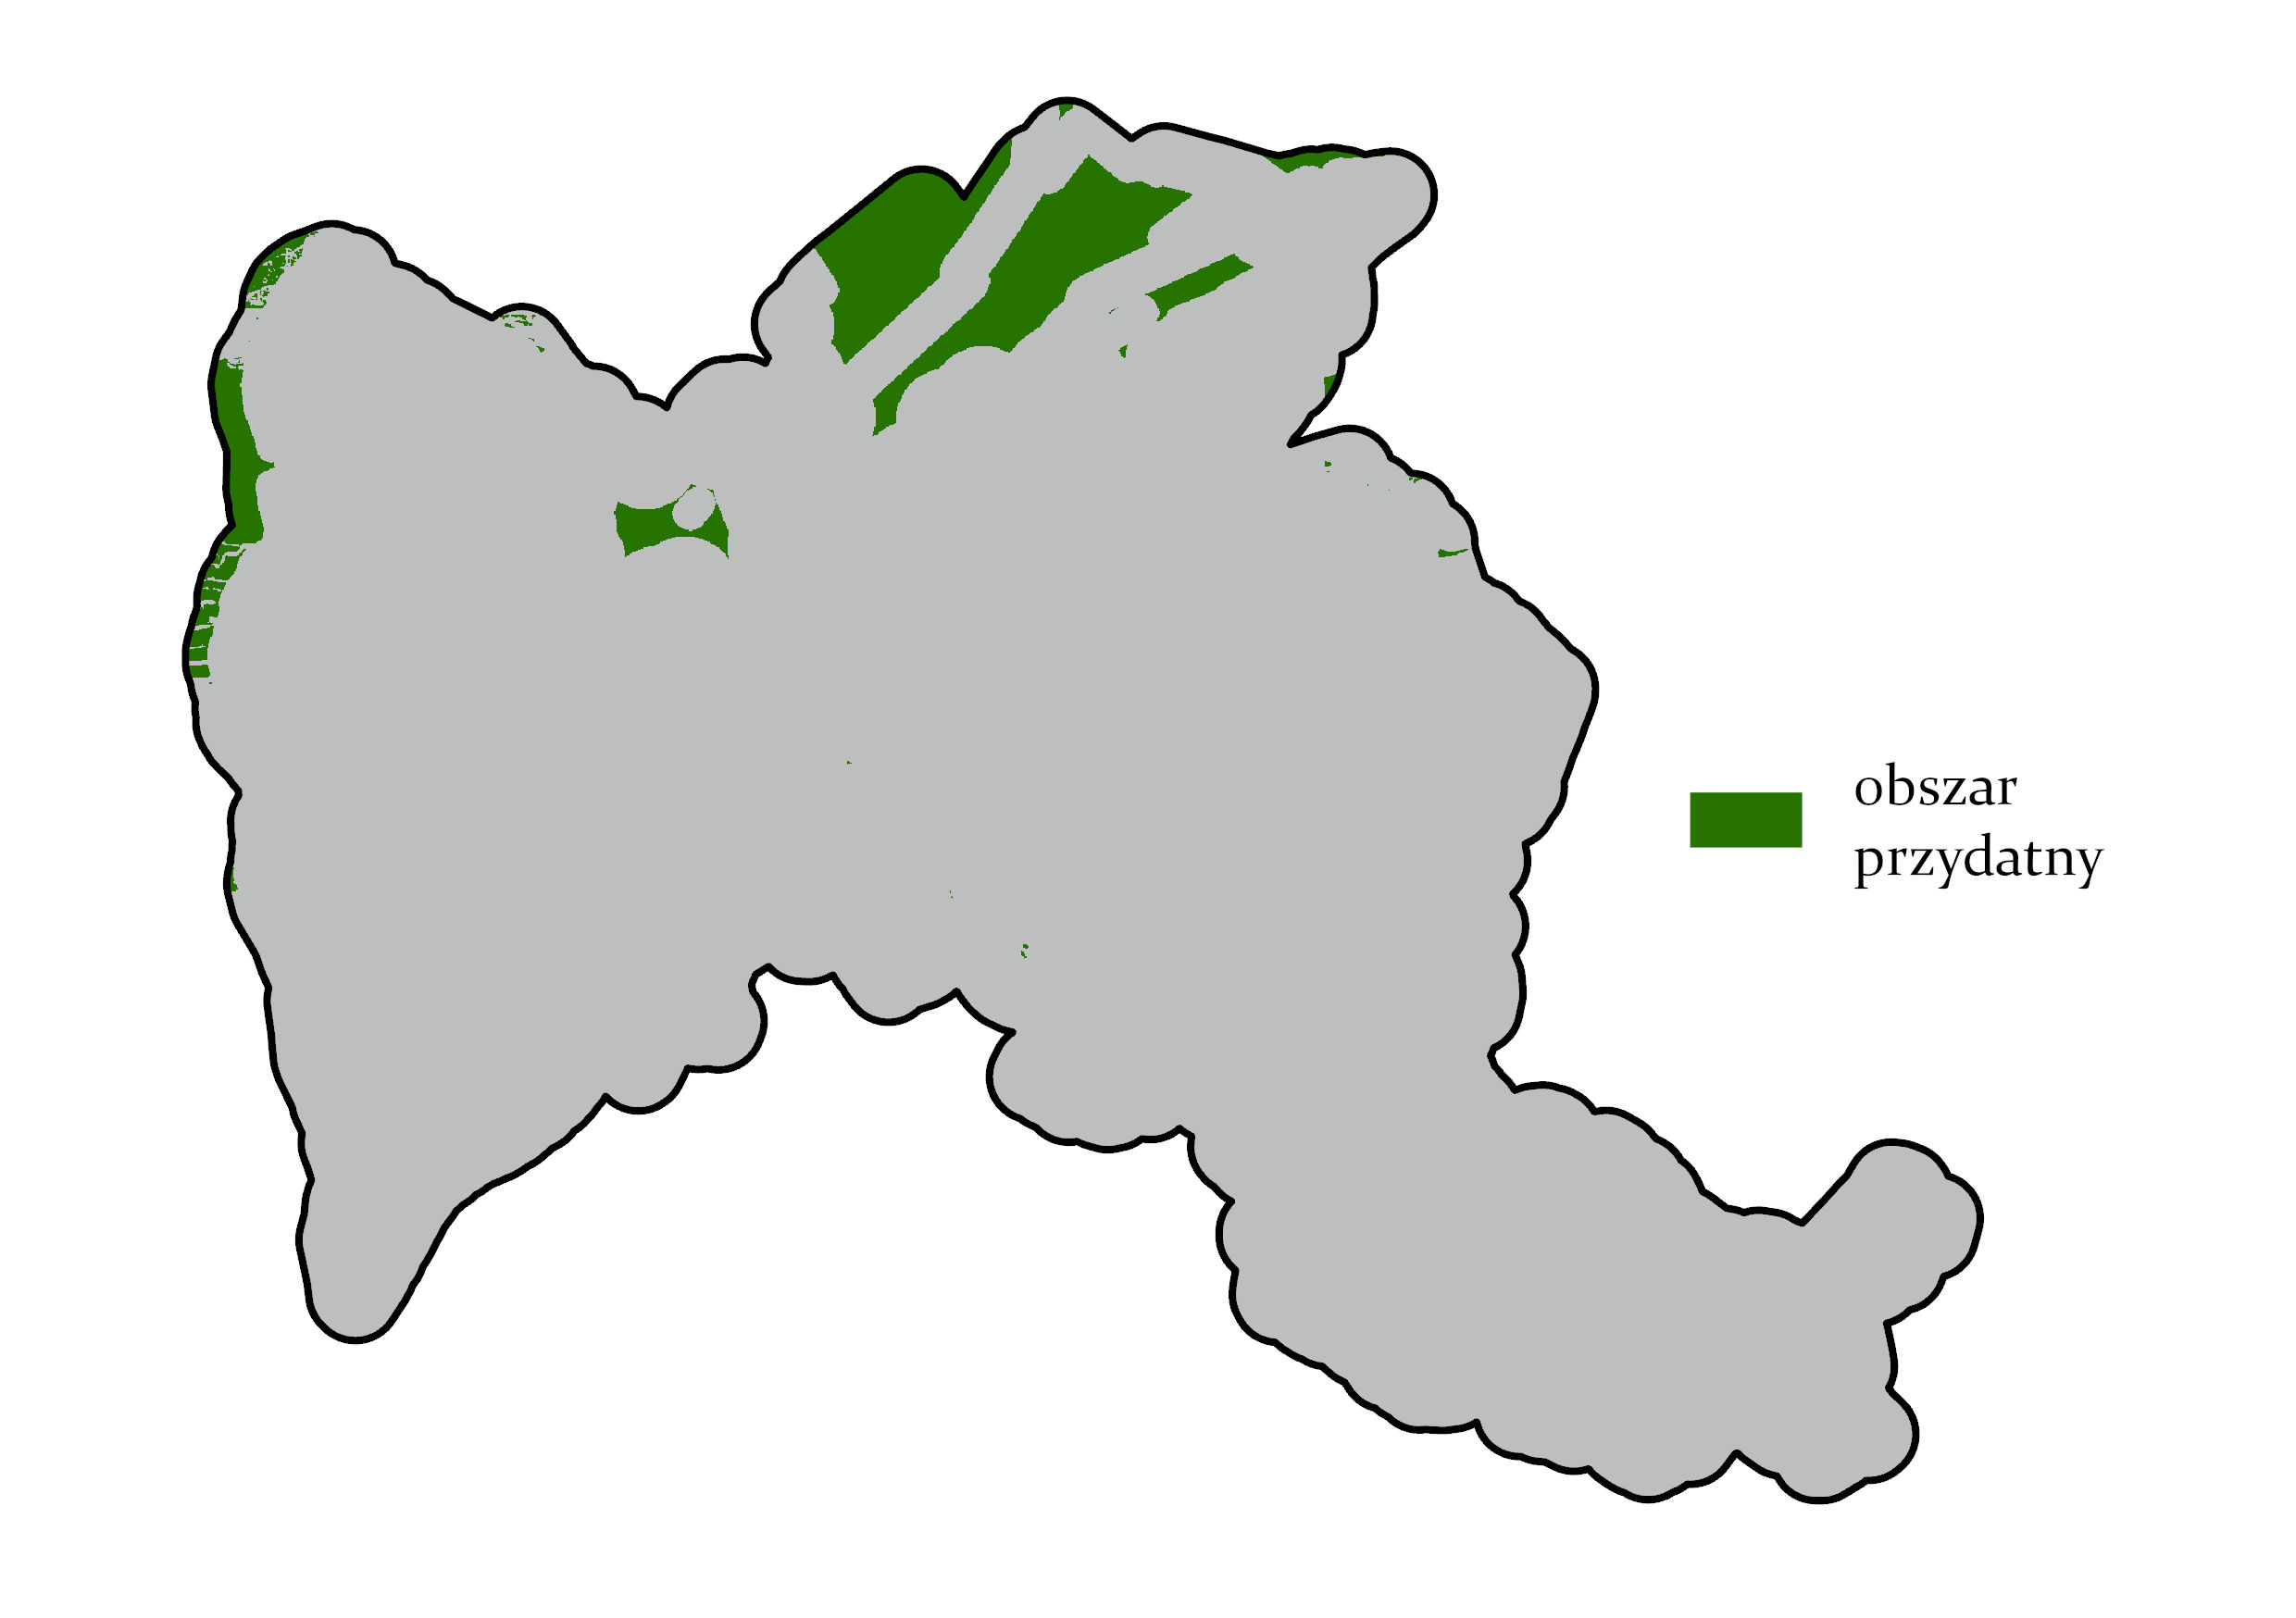
\includegraphics[width=\linewidth]{img/wynik-po-reklasyfikacji.jpg}
        \caption{Wynik łączenia kryteriów ostrych i rozmytych po reklasyfikacji - wagi równe}
        \label{fig:wynik-reklasyfikacja-rowne}
    \end{minipage}
    \hfill
    \begin{minipage}[t]{0.48\textwidth}
        \centering
        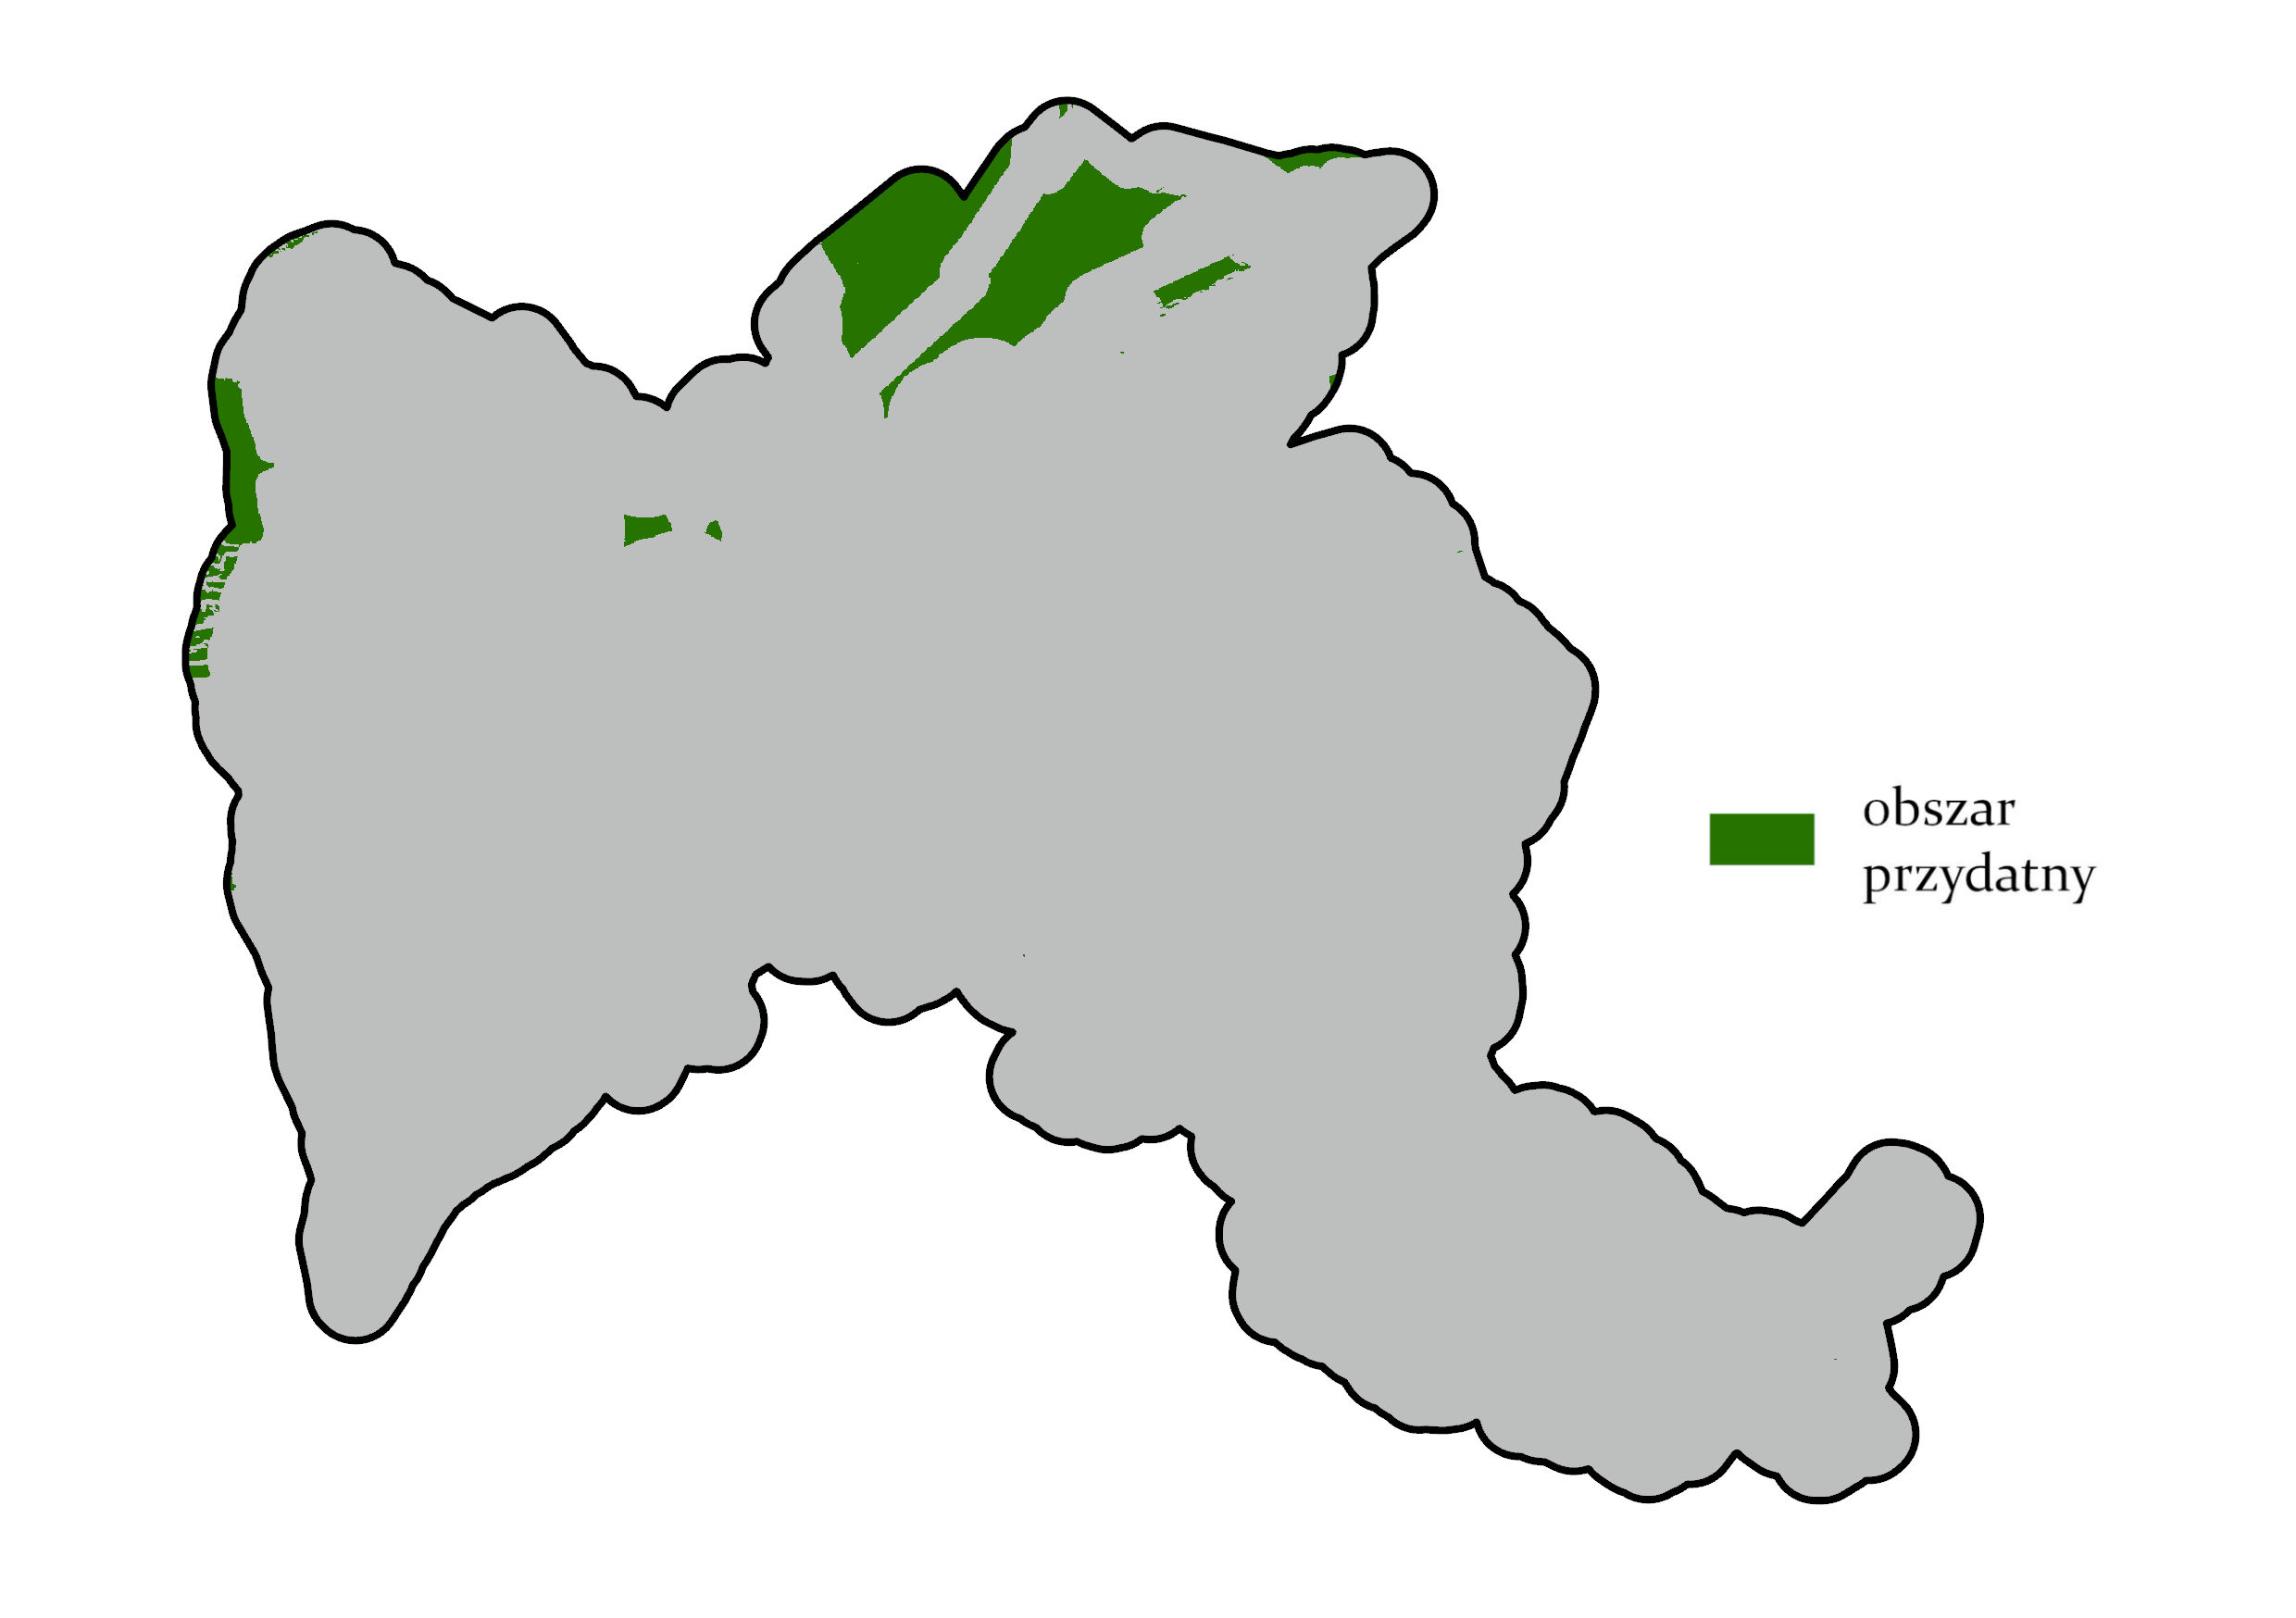
\includegraphics[width=\linewidth]{img/roznewagi-wynik-po-reklasyfikacji.jpg}
        \caption{Wynik łączenia kryteriów ostrych i rozmytych po reklasyfikacji - wagi różne}
        \label{fig:wynik-reklasyfikacja-rozne}
    \end{minipage}
\end{figure}

\newpage

\subsection{Wybór przydatnych działek}
Kod najpierw zamienia uzyskany wcześniej raster na warstwę poligonową. Następnie zostają wybrane tylko te poligony, które stanowią teren przydatny.

Później warstwa z działkami zostaje przecięta powstałymi poligonami. Dzięki temu działka zostaje podzielona na części przydatne i nieprzydatne. Kolejno, aby uzyskać procentową przydatność każdej z działek, pętla przechodzi przez warstwę z działkami przeciętymi oraz pierwotną warstwę z działkami. 
Jeżeli pętla natrafi na część przydatną działki, zostaje znaleziona odpowiednia działka w warstwie pierwotnej, i pole części przydatnej działki zostaje dodane do pola pole\_przydatne.

Dzięki temu możemy obliczyć przydatność działki - stosunek powierzchni przydatnej do powierzchni całkowitej. Wybieramy jedynie te działki, których przydatność jest wyższa od wybranego progu przydatności oraz takie, które mają powierzchnię co najmniej 2ha.

\begin{mintedbox}{python}
arcpy.conversion.RasterToPolygon(f'{geobaza}\\{wariant}_wynik_reclassified', 'poligon_przydatnosci', "NO_SIMPLIFY", "VALUE")
arcpy.management.MakeFeatureLayer('poligon_przydatnosci', "poligon_przydatnosci_layer")
arcpy.management.SelectLayerByAttribute("poligon_przydatnosci_layer", "NEW_SELECTION", "gridcode = 1")
arcpy.management.CopyFeatures("poligon_przydatnosci_layer", f"{geobaza}\\{wariant}_poligon_przydatnosci")

arcpy.analysis.SummarizeWithin(
    in_polygons=dzialki,
    in_sum_features=f"{geobaza}\\{wariant}_poligon_przydatnosci",
    out_feature_class=f'{geobaza}\\{wariant}_summarized_within',
    keep_all_polygons="ONLY_INTERSECTING",
    shape_unit="SQUAREMETERS",
    add_group_percent="NO_PERCENT",
)

arcpy.management.CalculateField(
    in_table=f'{geobaza}\\{wariant}_summarized_within',
    field="pow_przyd",
    expression="100*!sum_Area_squaremeters!/!Shape_Area!",
    expression_type="PYTHON3",
    code_block="",
    field_type="FLOAT"
)

dzialki_przydatne_powyzej_progu = arcpy.management.SelectLayerByAttribute(f'{geobaza}\\{wariant}_summarized_within', "NEW_SELECTION", f"pow_przyd >= 60")
arcpy.management.CopyFeatures(dzialki_przydatne_powyzej_progu, f"{geobaza}\\{wariant}_dzialki_przydatne_powyzej")

arcpy.management.Dissolve(
in_features=f"{geobaza}\\{wariant}_dzialki_przydatne_powyzej",
out_feature_class=f"{geobaza}\\{wariant}_dzialki_przydatne_powyzej_dissolve",
multi_part="SINGLE_PART",
unsplit_lines="DISSOLVE_LINES",
concatenation_separator=""
)
arcpy.management.MakeFeatureLayer(f"{geobaza}\\{wariant}_dzialki_przydatne_powyzej_dissolve", f"{geobaza}\\{wariant}_dzialki_przydatne_powyzej_dissolve_layer")
arcpy.management.SelectLayerByAttribute(f"{geobaza}\\{wariant}_dzialki_przydatne_powyzej_dissolve_layer", "NEW_SELECTION", "Shape_Area >= 20000")
arcpy.management.CopyFeatures(f"{geobaza}\\{wariant}_dzialki_przydatne_powyzej_dissolve_layer", f"{geobaza}\\{wariant}_grupy_dzialek_przydatne_powyzej_{prog_przydatnosci}")
\end{mintedbox}

\begin{figure}[H]
    \begin{minipage}[t]{0.48\textwidth}
        \centering
        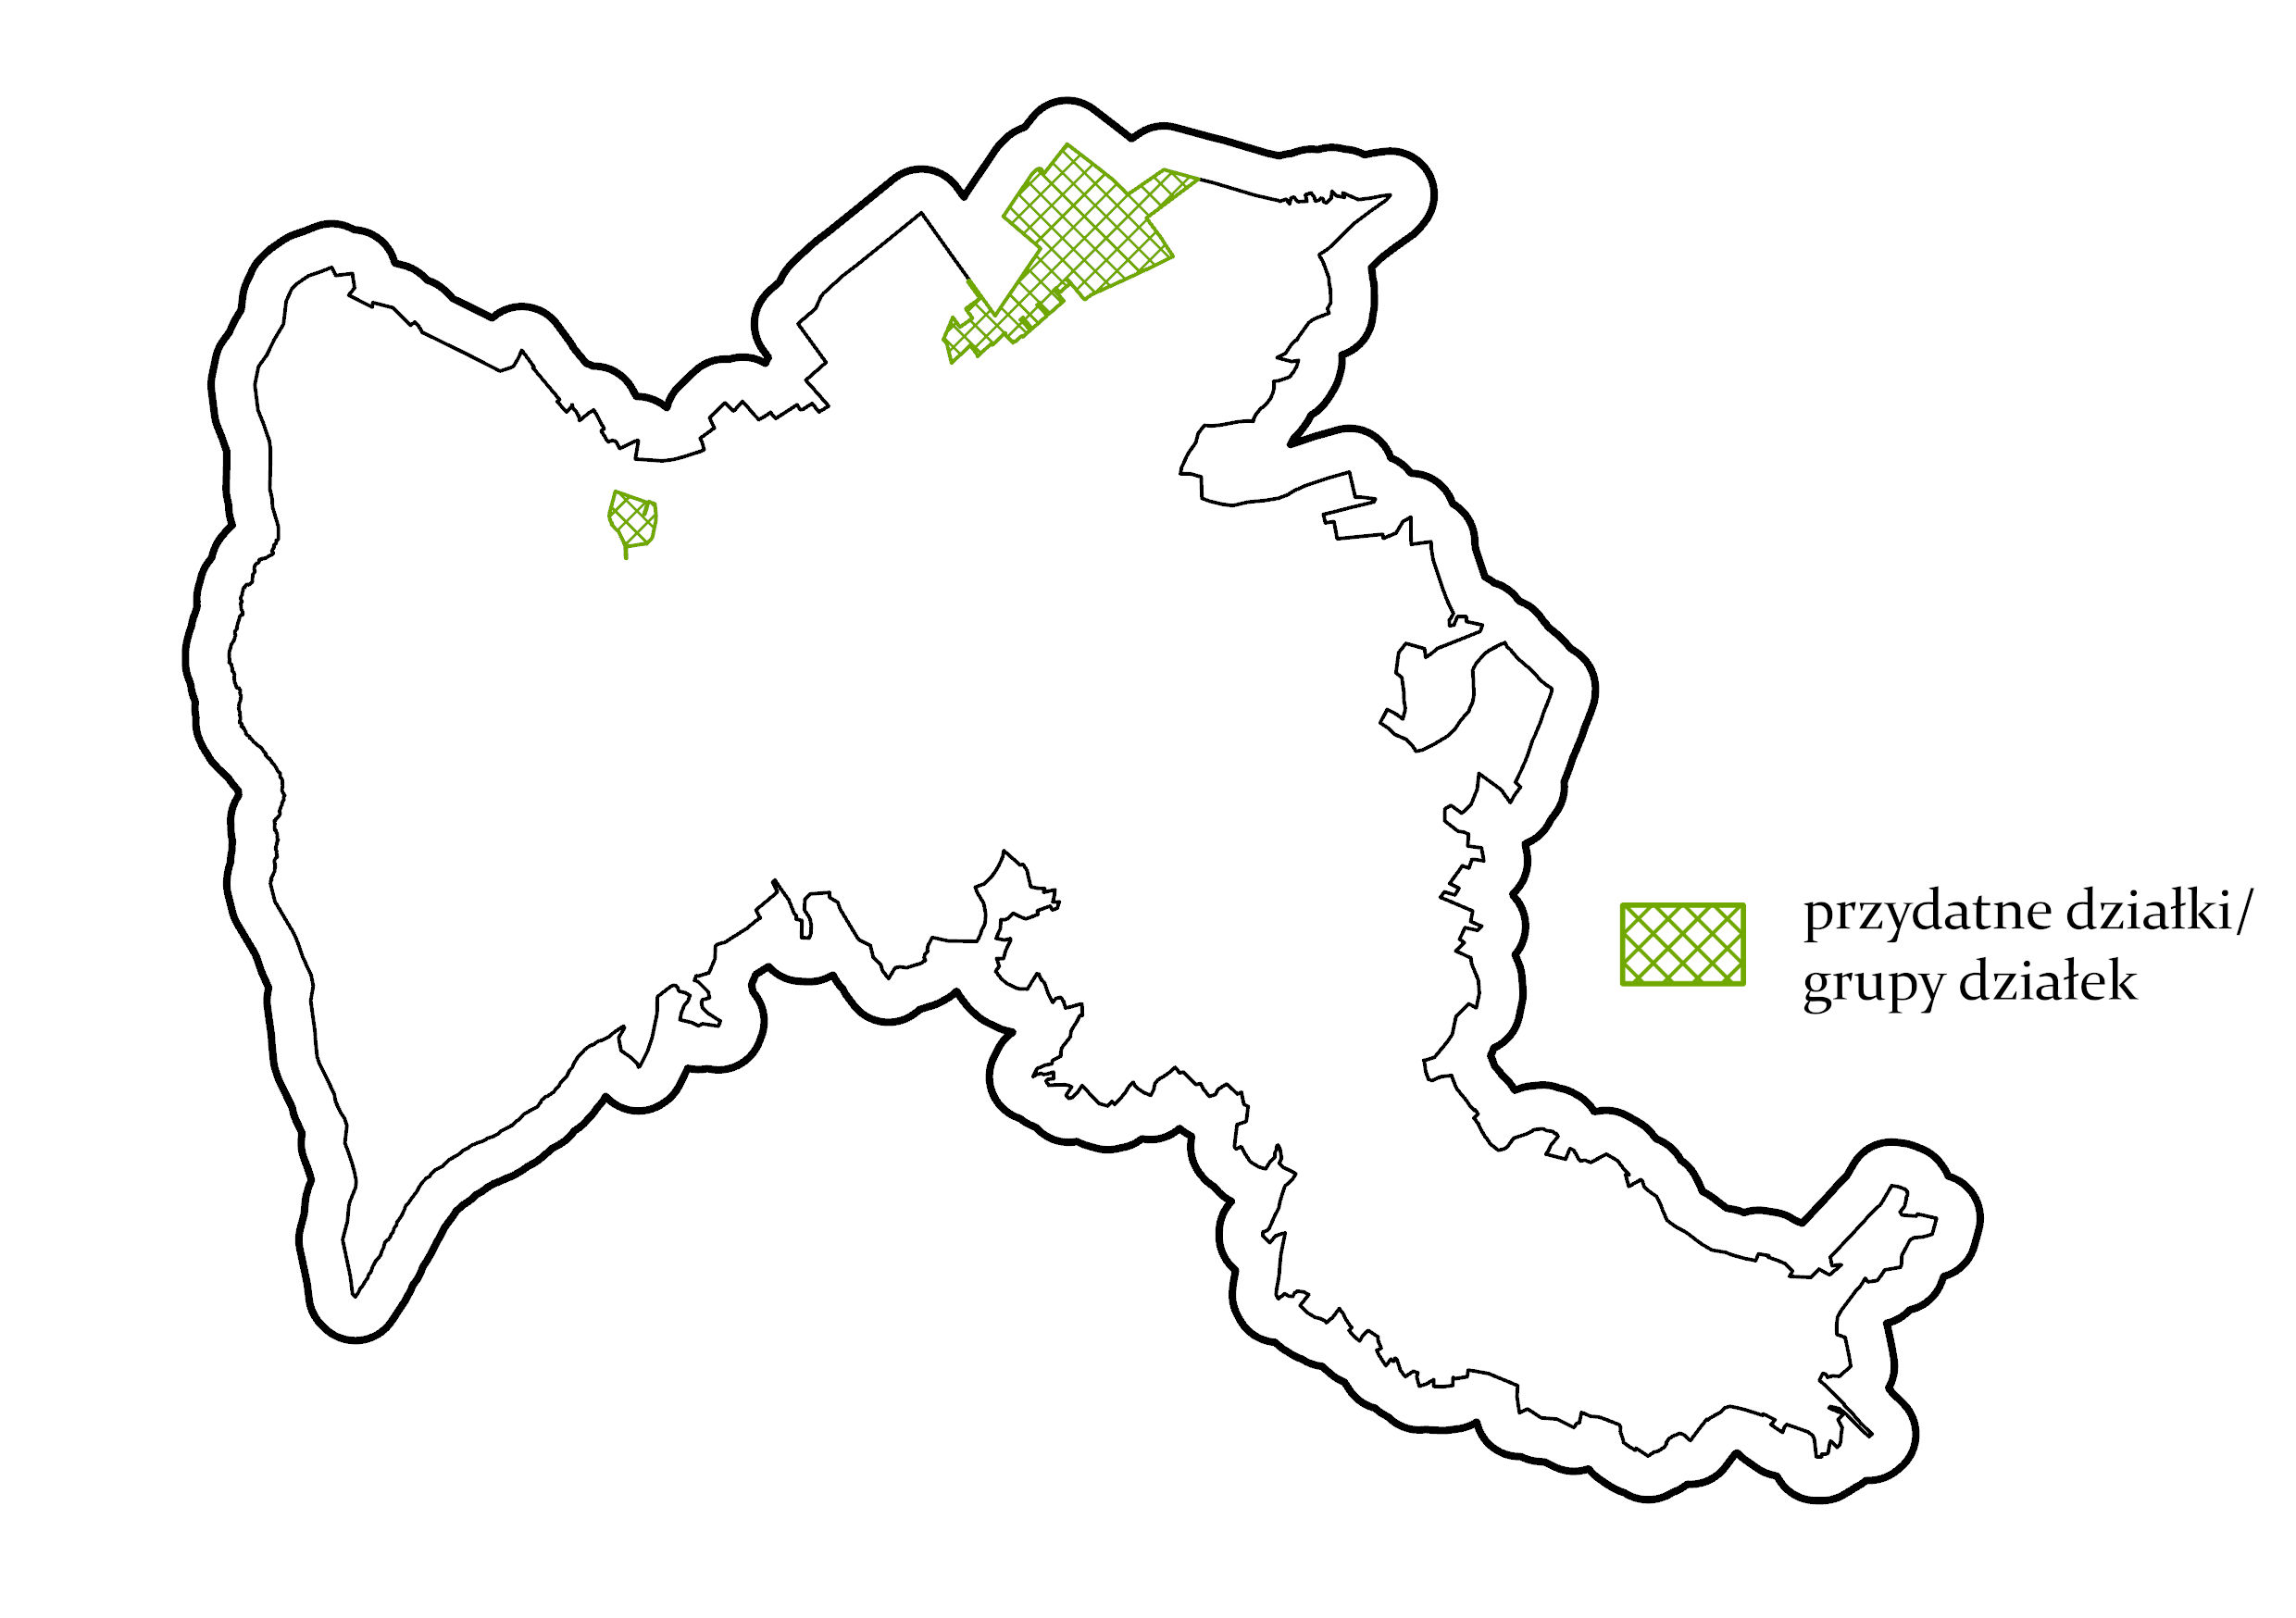
\includegraphics[width=\linewidth]{img/przydatne-dzialki.jpg}
        \caption{Mapa przedstawiająca przydatne działki - wagi równe}
        \label{fig:przydatne-dzialki-rowne}
    \end{minipage}
    \hfill
    \begin{minipage}[t]{0.48\textwidth}
        \centering
        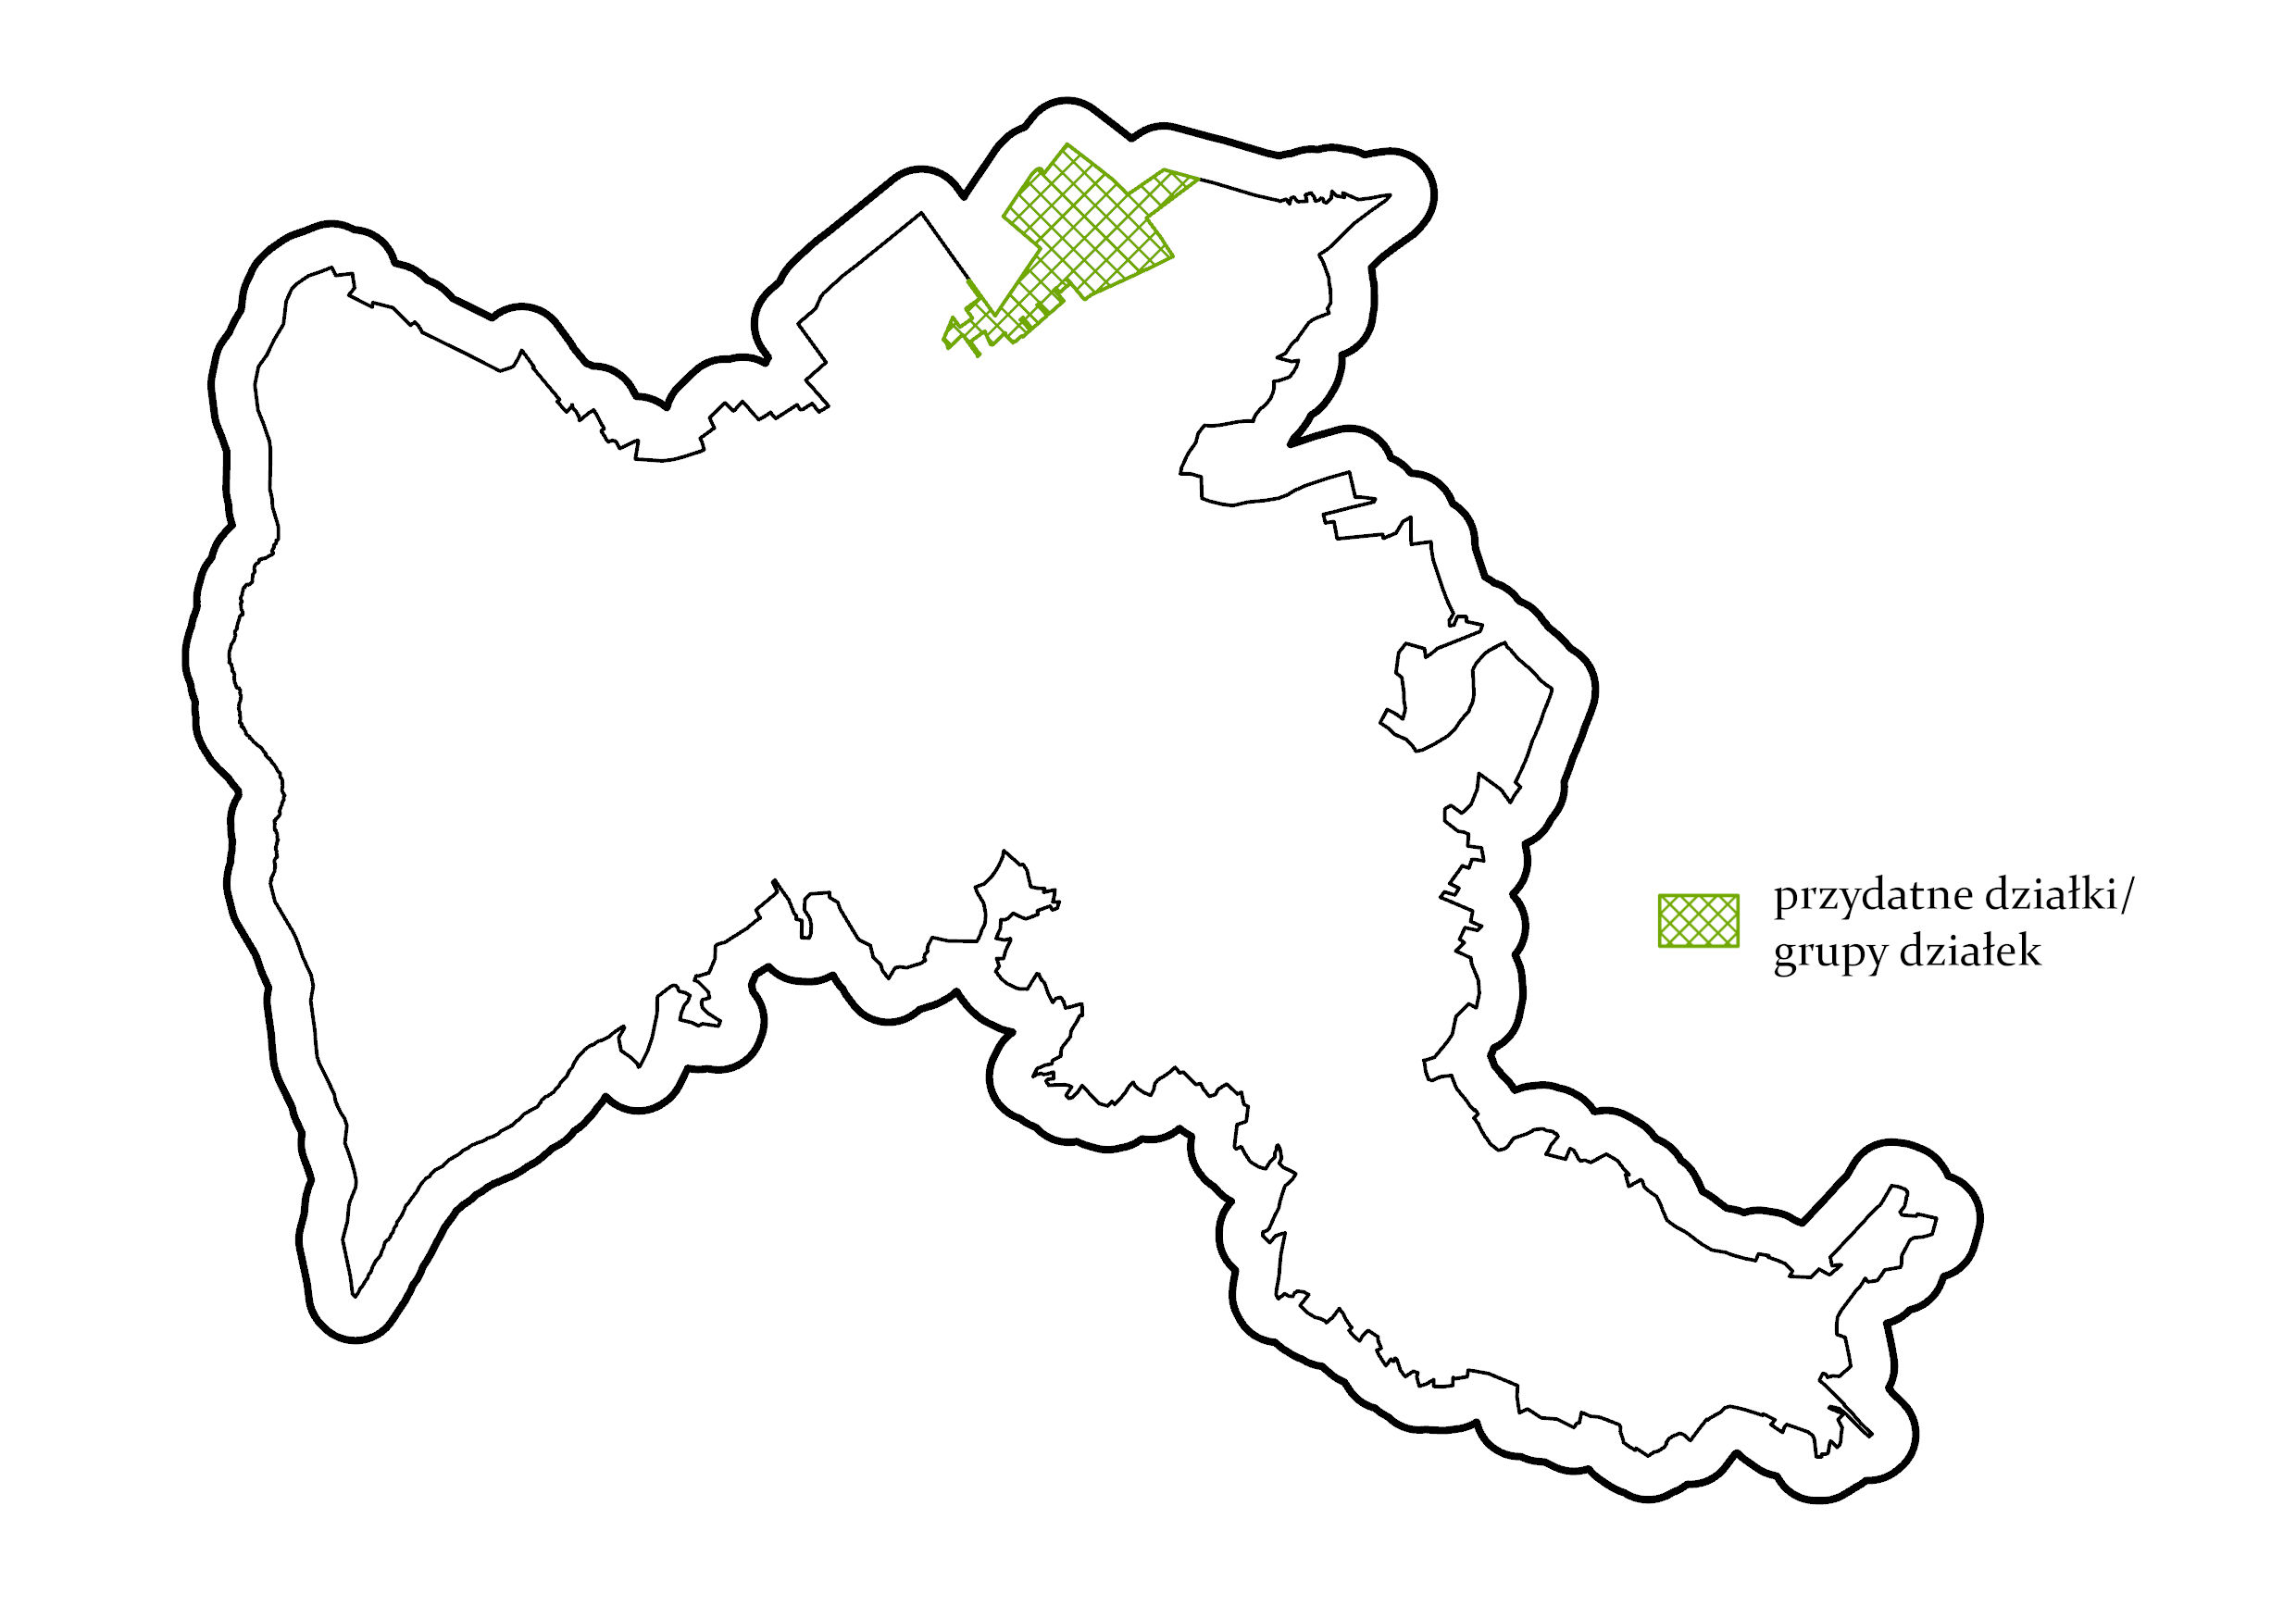
\includegraphics[width=\linewidth]{img/roznewagi-przydatne-dzialki.jpg}
        \caption{Mapa przedstawiająca przydatne działki - wagi różne}
        \label{fig:przydatne-dzialki-rozne}
    \end{minipage}
\end{figure}


\begin{figure}[H]
    \begin{minipage}[t]{0.48\textwidth}
        \centering
        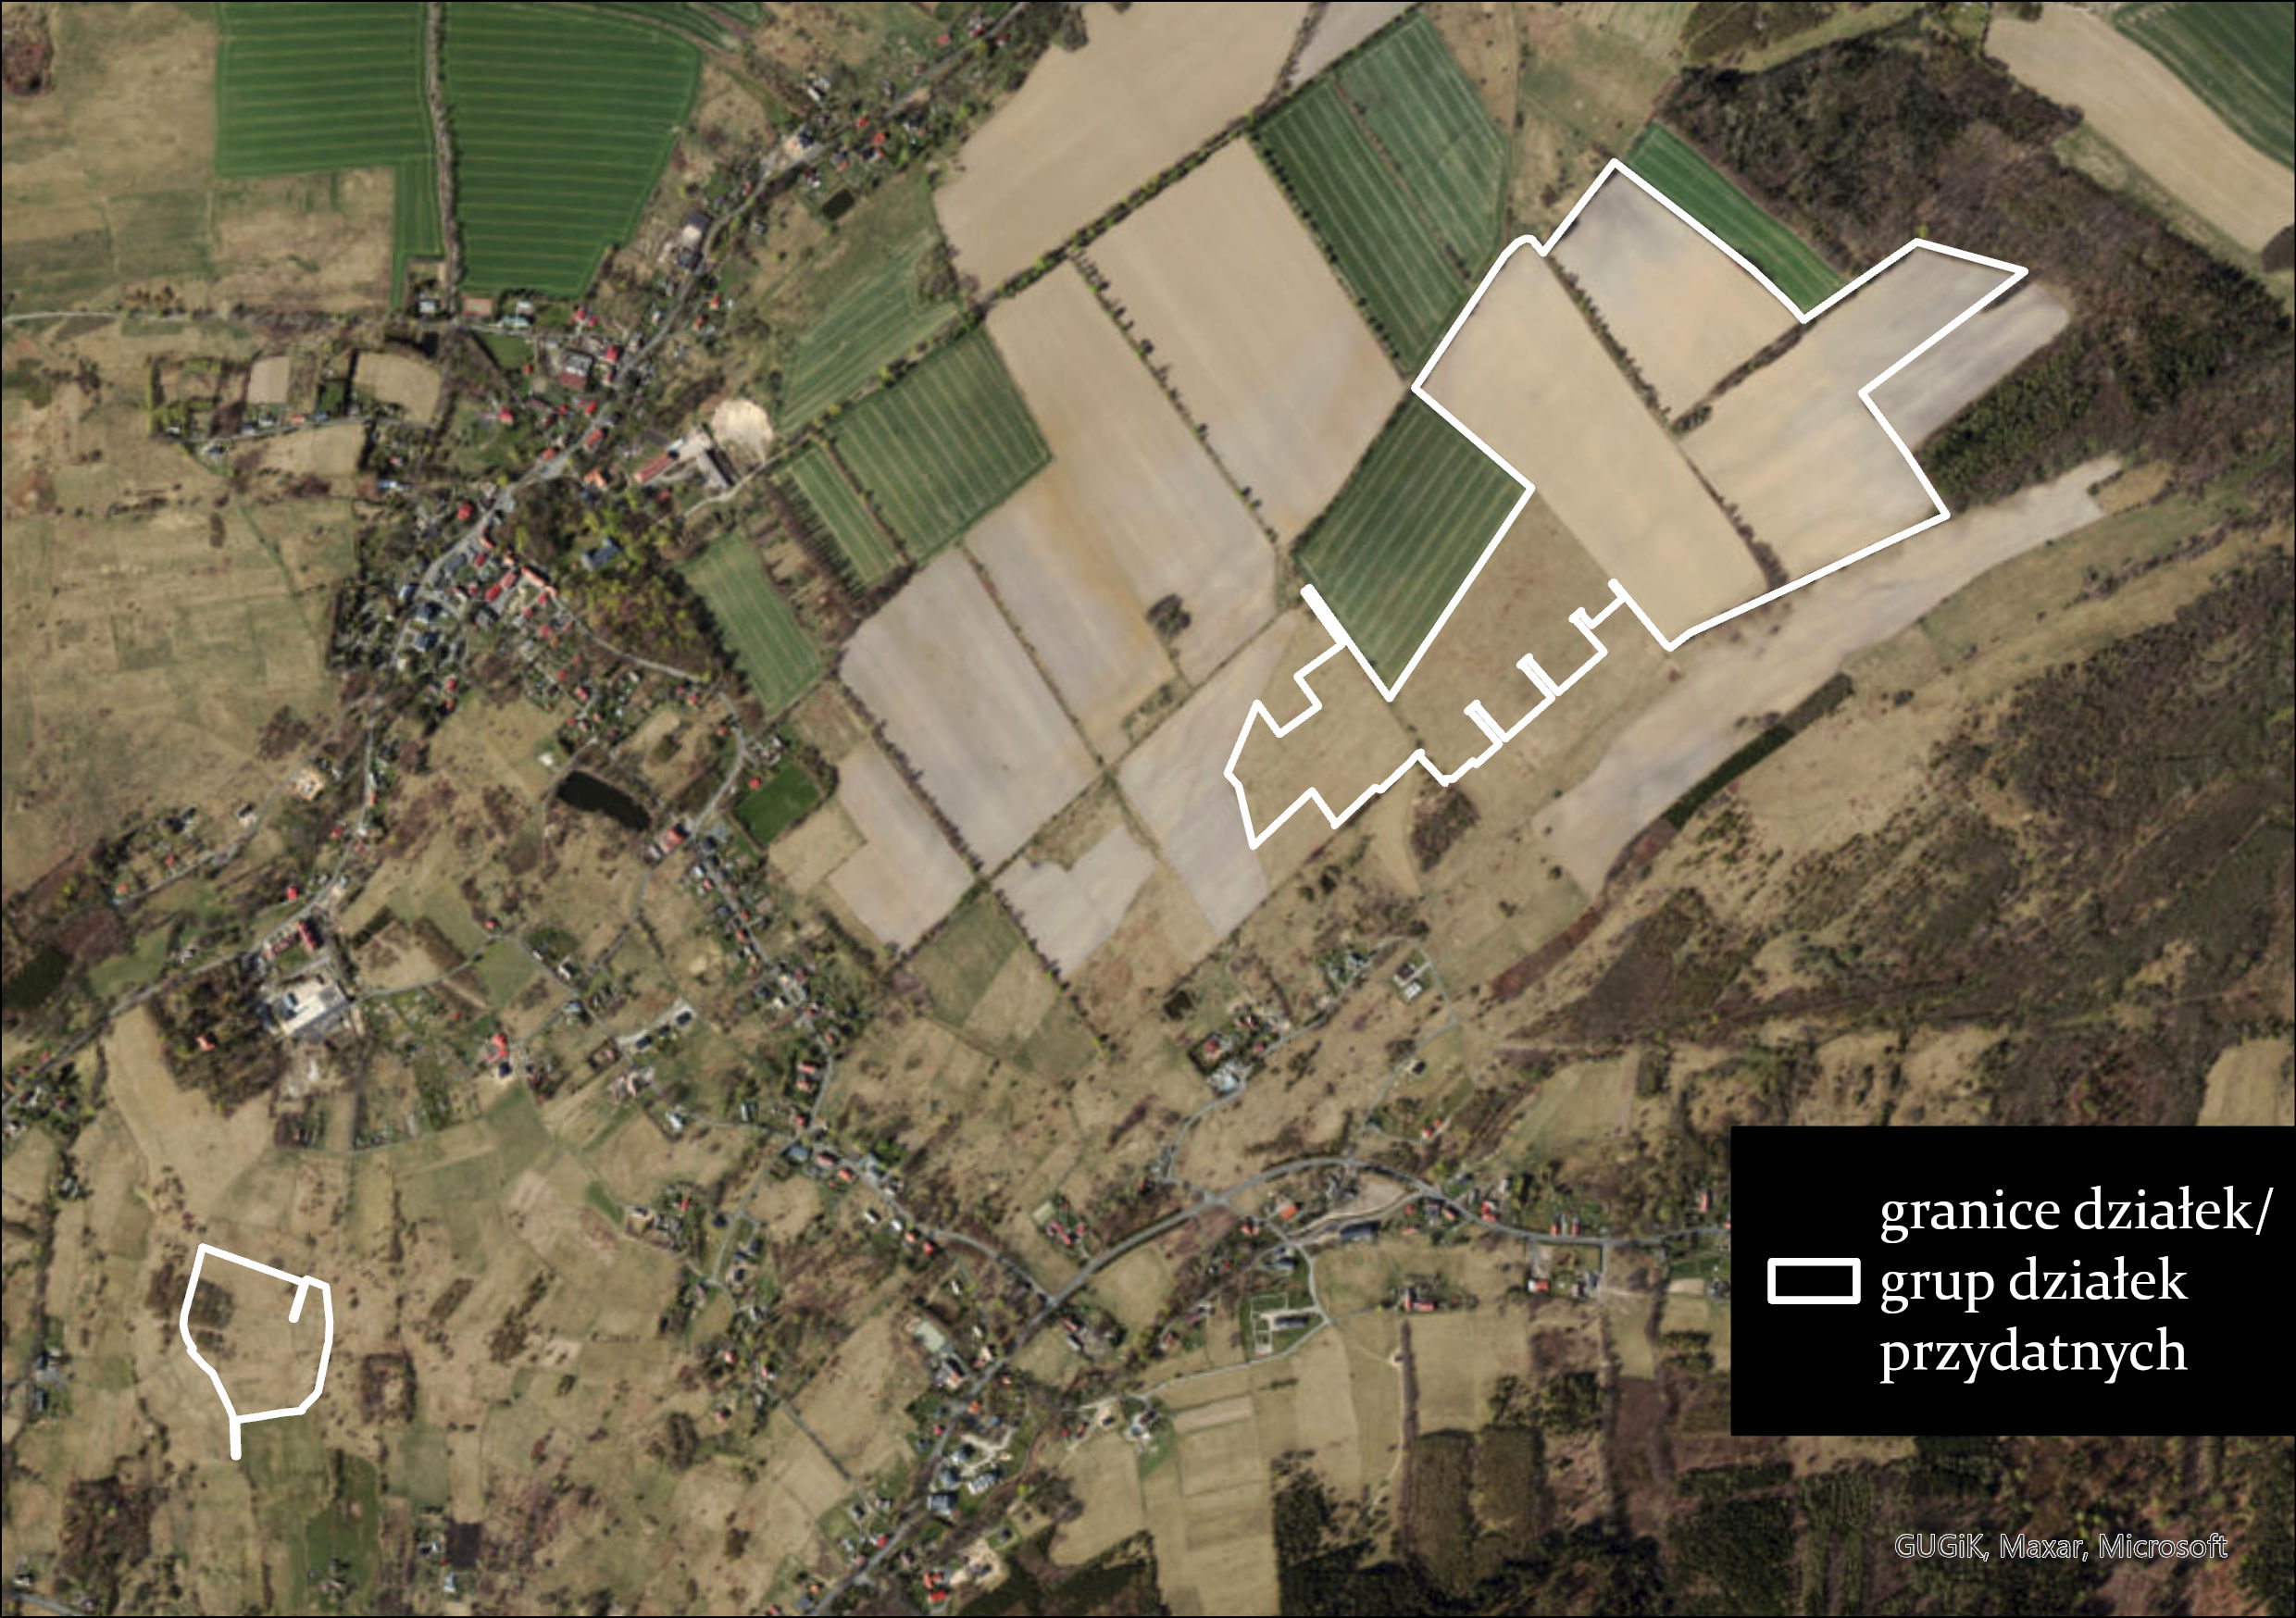
\includegraphics[width=\linewidth]{img/dzialki-przydatne-ortofoto.jpg}
        \caption{Mapa przedstawiająca przydatne działki na ortofotomapie - wagi równe}
        \label{fig:dzialki-ortofoto-rowne}
    \end{minipage}
    \hfill
    \begin{minipage}[t]{0.48\textwidth}
        \centering
        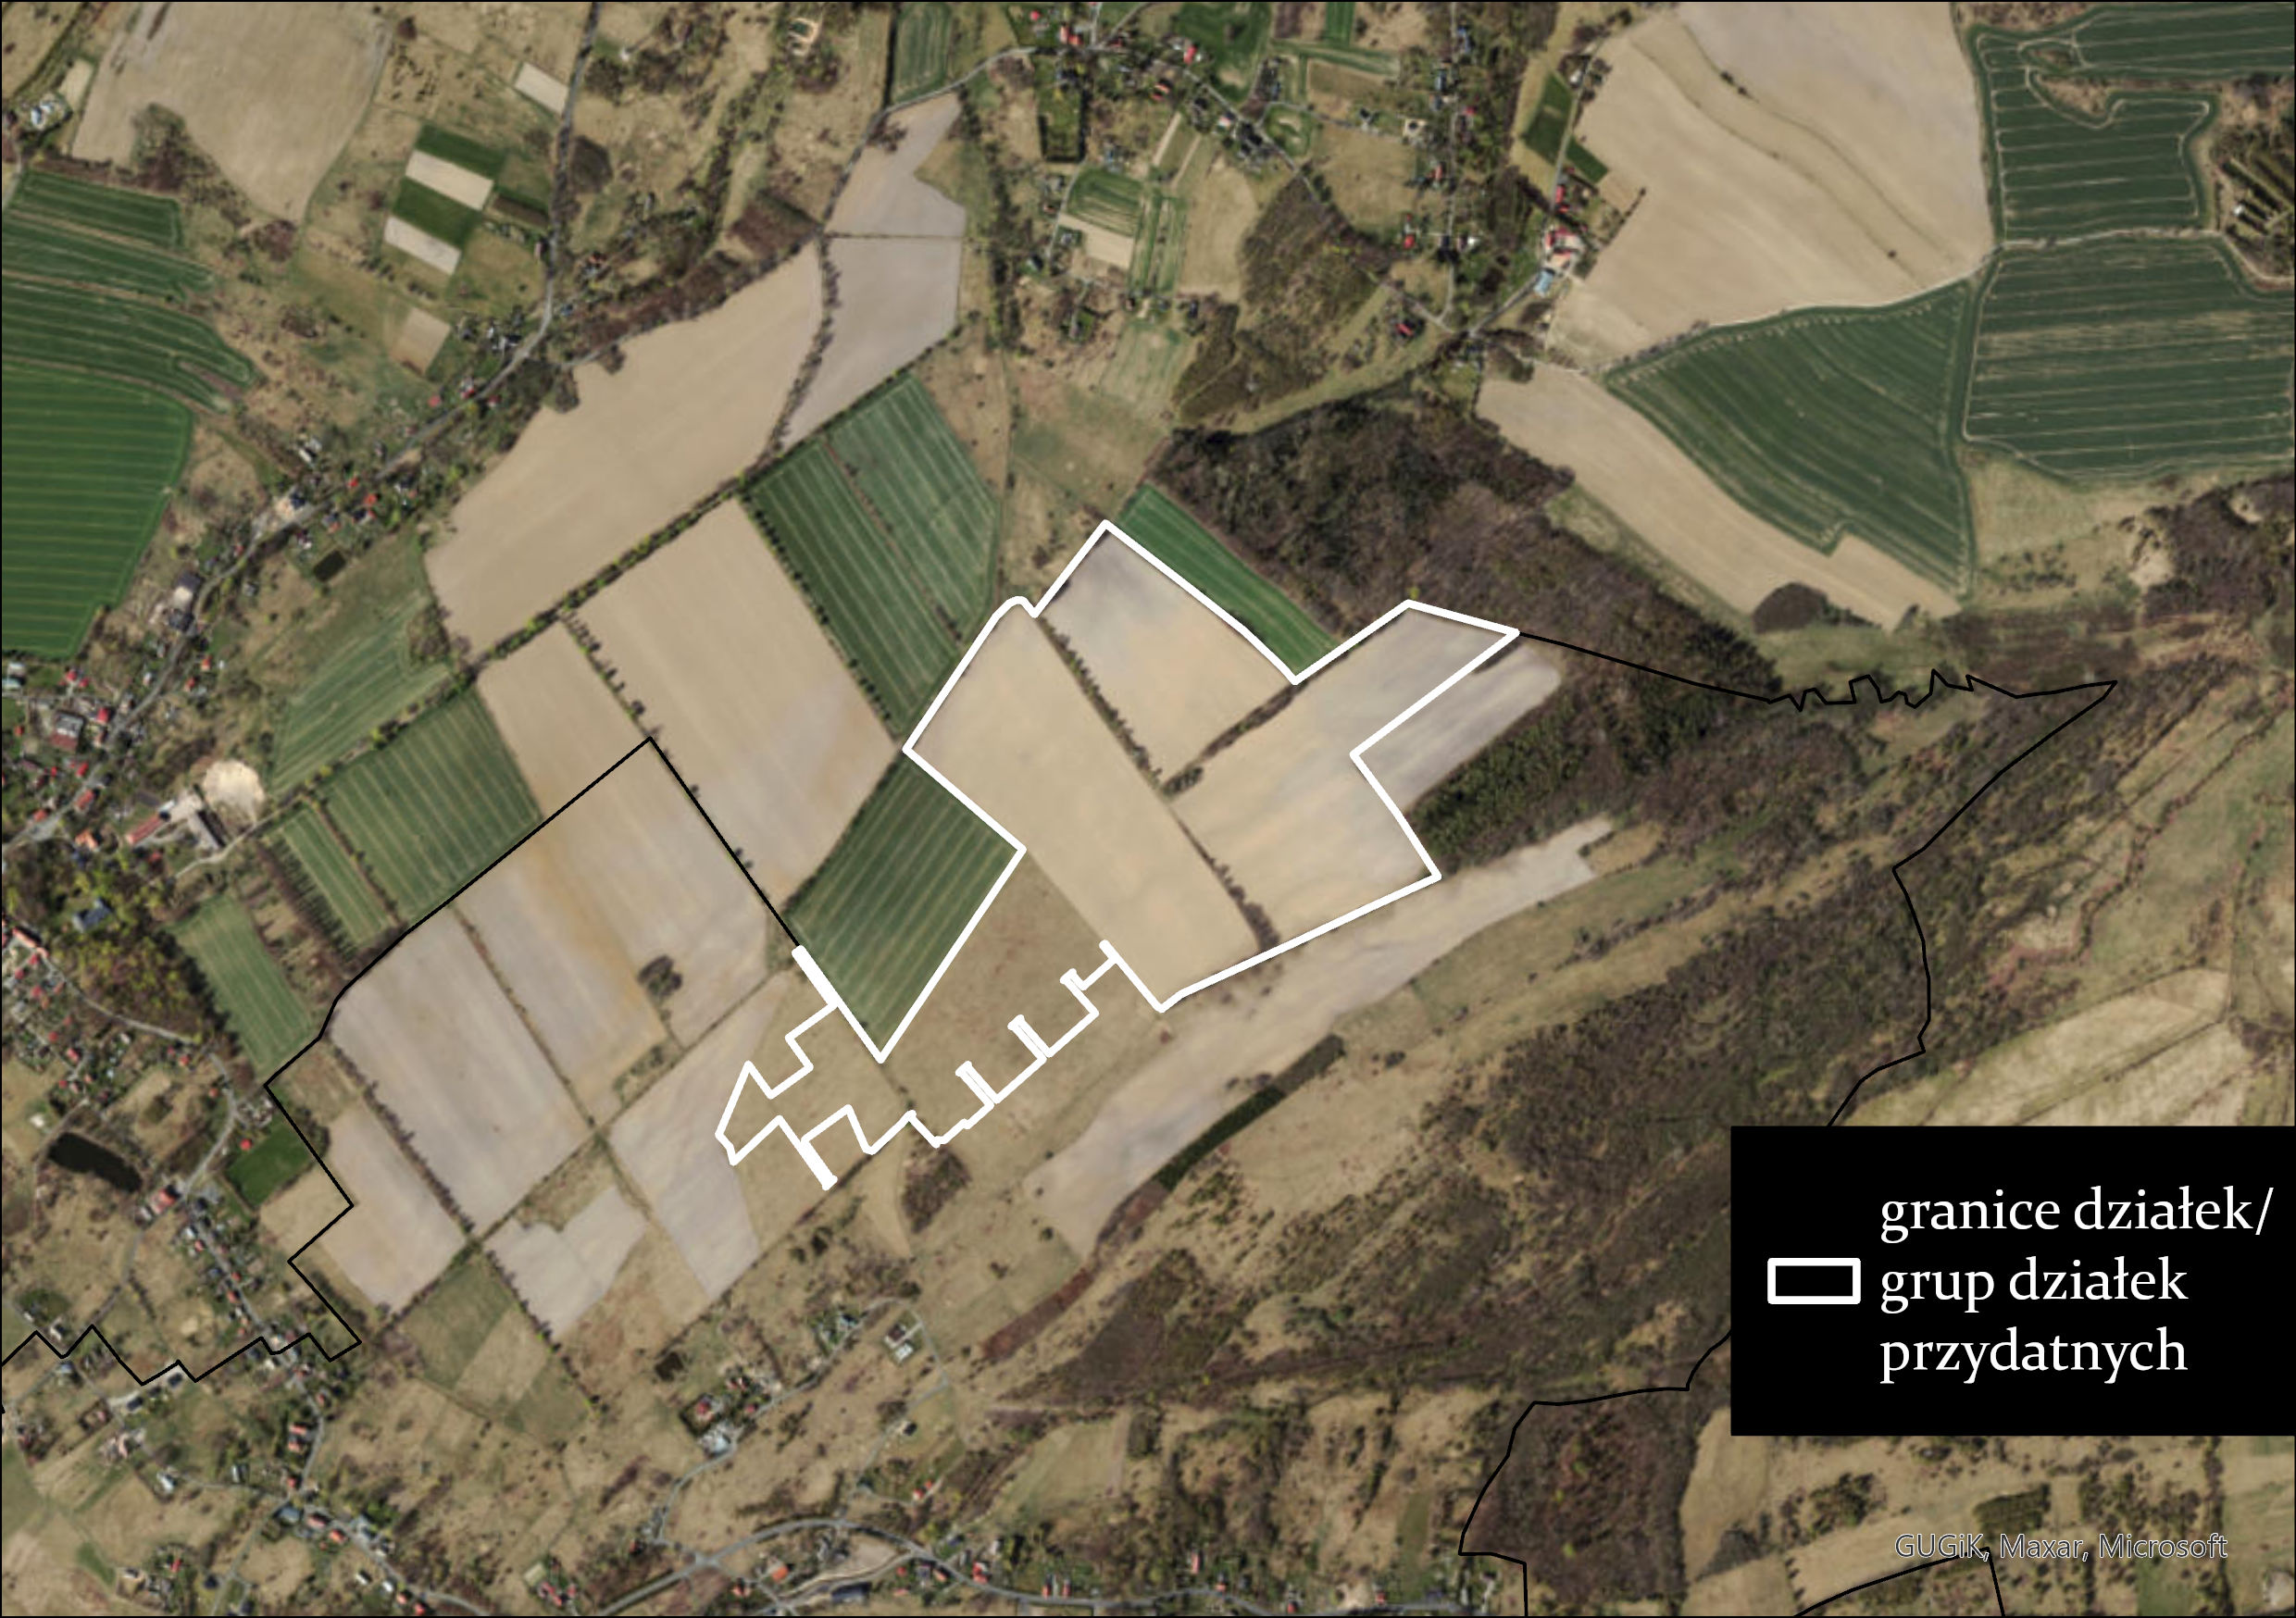
\includegraphics[width=\linewidth]{img/roznewagi-dzialki-przydatne-ortofoto.jpg}
        \caption{Mapa przedstawiająca przydatne działki na ortofotomapie - wagi różne}
        \label{fig:dzialki-ortofoto-rozne}
    \end{minipage}
\end{figure}


\subsection{Koszt przyłącza do sieci SN}
Przed rozpoczęciem analiz należało stworzyć tzw. mapę kosztów względnych(jednostkowych), która przedstawia faktyczną lub umowną wartość kosztu zbudowania
przyłącza przez dany obszar. Dla mapy kosztów względnych w postaci rastrowej, będzie to względny koszt budowy przyłącza na obszarze o powierzchni odpowiadającej rozmiarowi
piksela. W ćwiczeniu przyjęto, że koszt = 1 jest odniesiony do obszarów rolniczych (najmniejszy koszt prac ziemnych / budowlanych dla 1 piksela). Koszty względne dla innych obszarów są obliczane jako wielokrotność kosztów dla terenów rolniczych. Przypisane koszty dla wszystkich kategorii użytkowania terenu dla doprowadzenia do
farmy przyłącza przedstawia tabela.

Następnie, dla każdego obiektu połączonej warstwy zawierającej pokrycie terenu gminy dodano odpowiedni koszt, na podstawie pola x\_kod, mówiącego o typie terenu, jaki stanowi. Warstwę nastepnie zamieniamy na raster, wykorzystując do tego nowo dodane pole z kosztem. Tworzymy mapę kosztów skumulowanych (cost map) oraz mapę kierunków (backlink raster) z użyciem narzędzia Cost Distance. Wykorzystując utworzone mapy, tworzymy ścieżkę przyłącza o najmniejszym koszcie (cost path). Rastrowa ścieżka zostaje przekonwertowana na warstwę wektorową.

\begin{figure}[H]
    \centering
    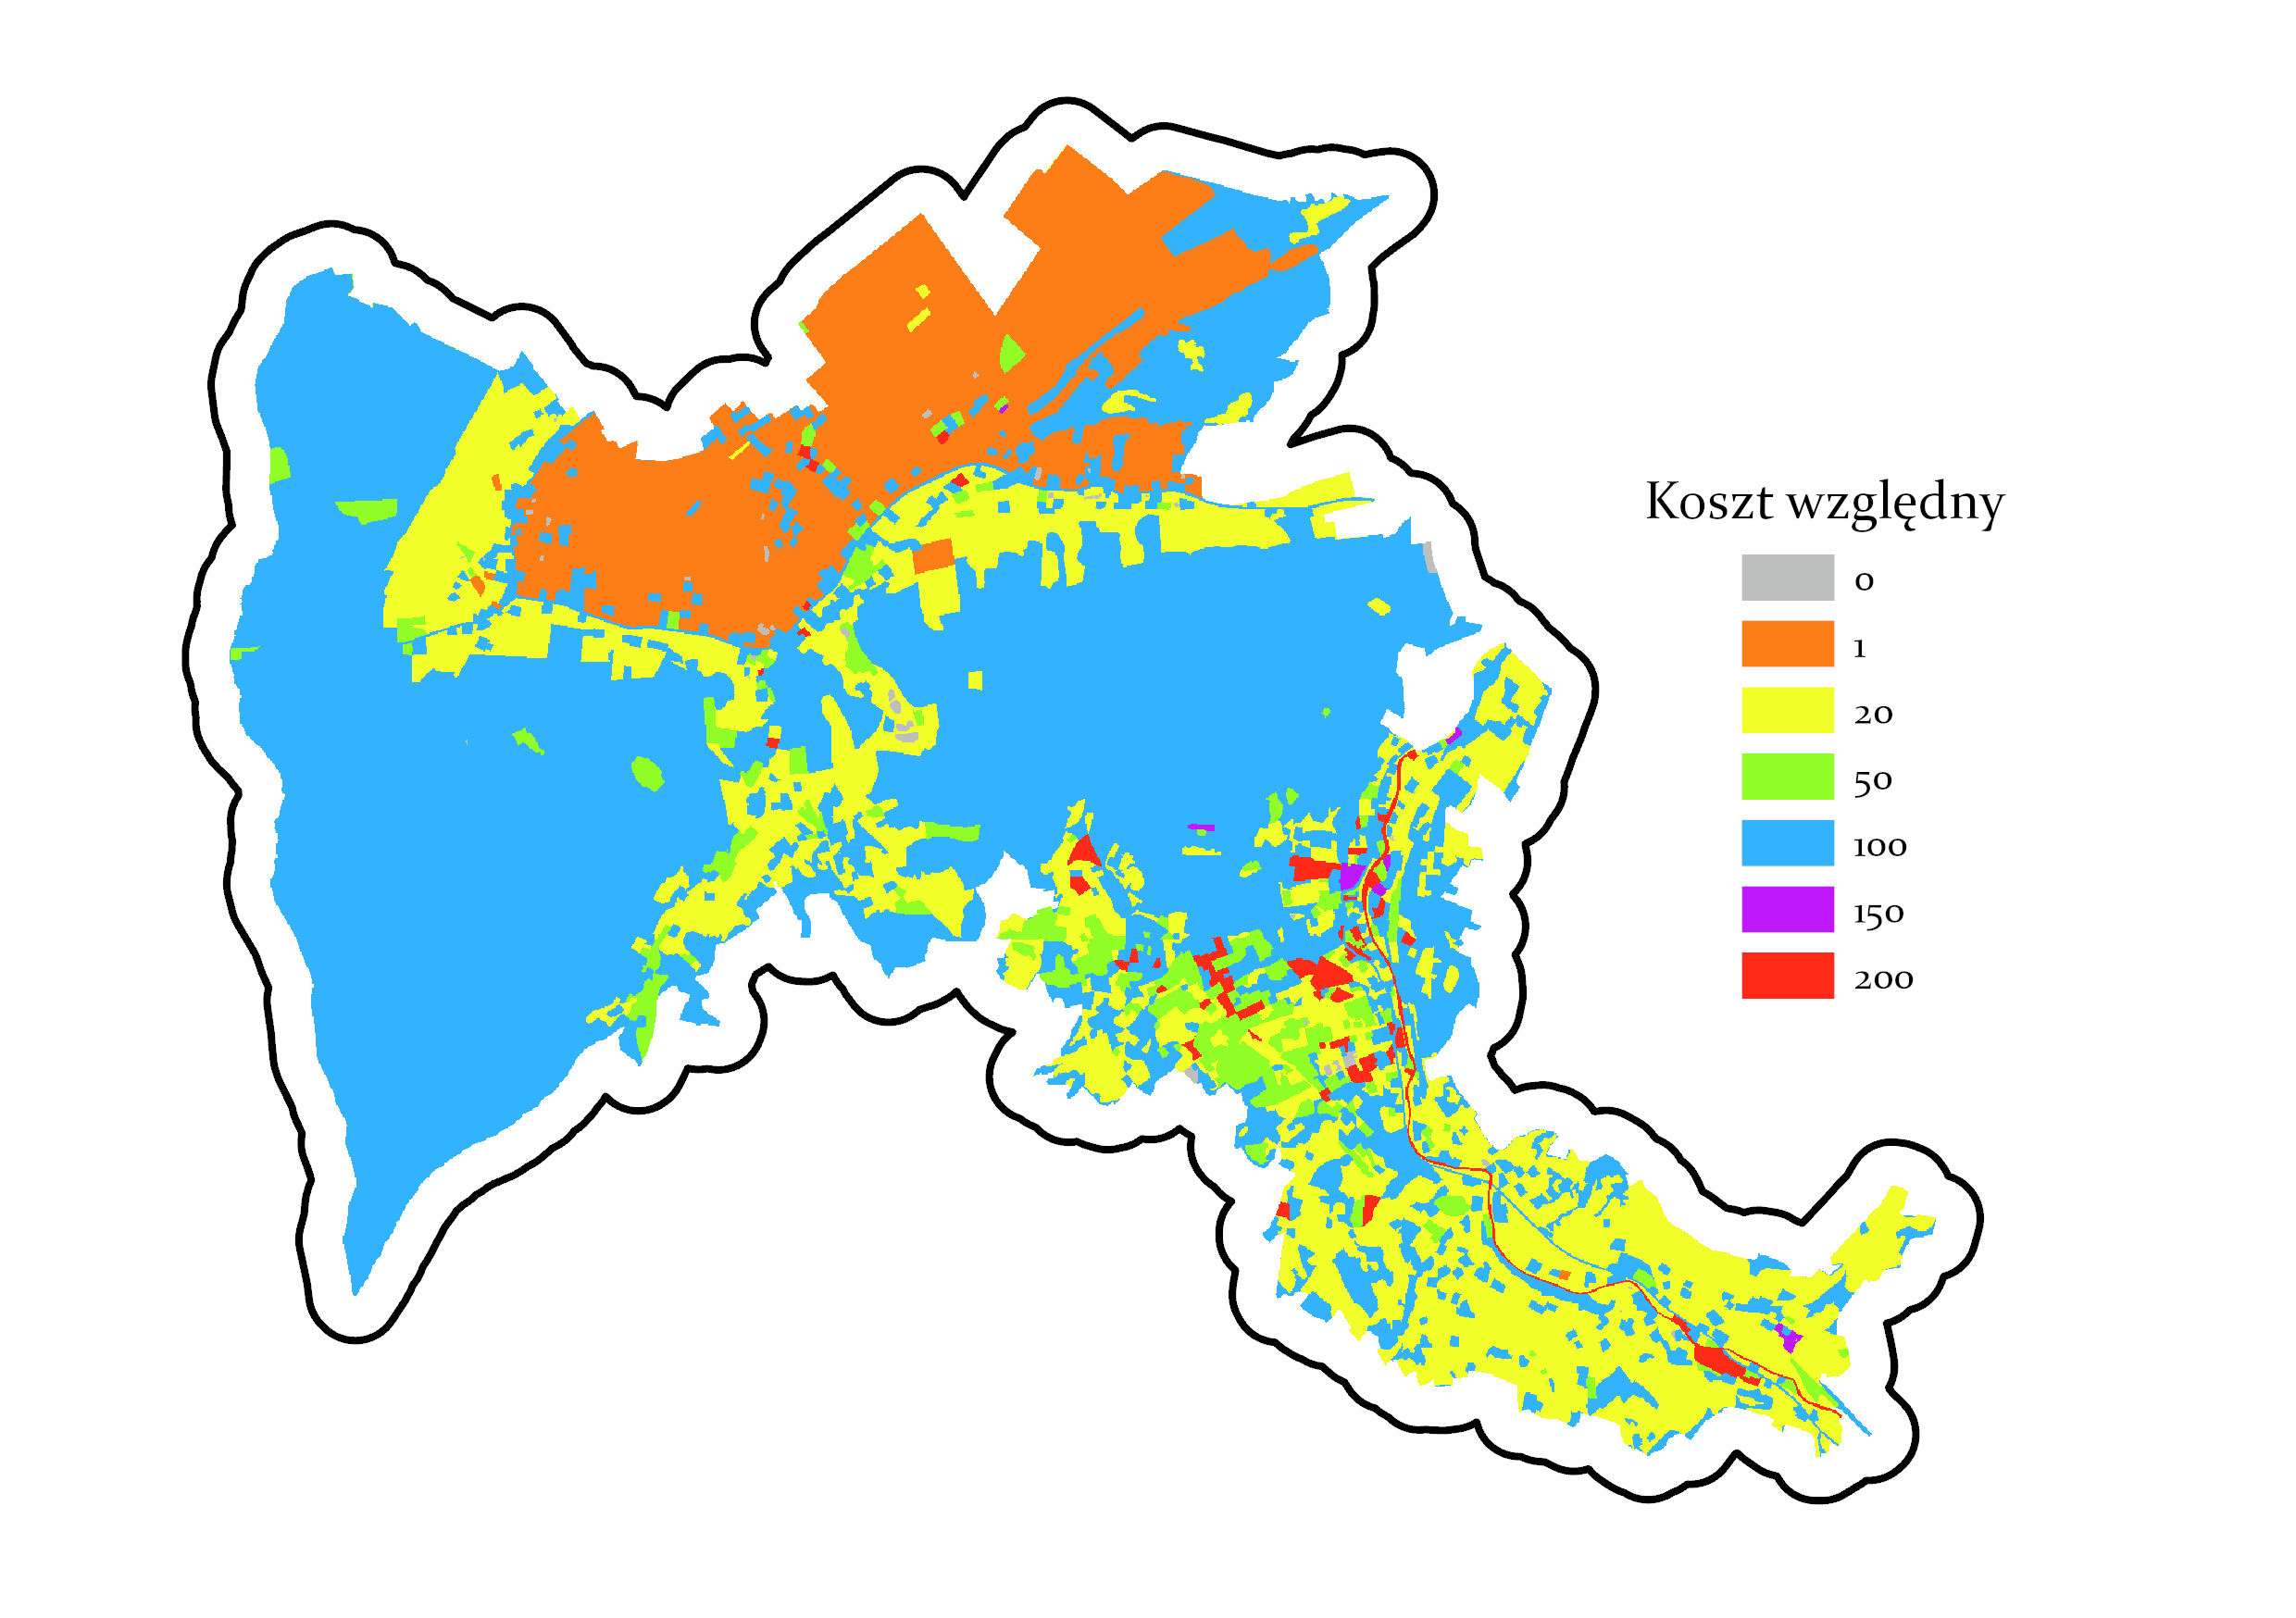
\includegraphics[width=0.75\textwidth]{img/cost-raster.jpg}
    \caption{Mapa kosztów względnych}
\end{figure}

% \begin{table}[ht]
%     \centering % Wyśrodkowanie tabeli
%     \renewcommand{\arraystretch}{1.2} % Zwiększenie odstępów między wierszami
%     \begin{tabular}{|p{2cm}|p{4.5cm}|p{2cm}|p{3cm}|p{2cm}|}
%     \hline
%     \textbf{Kod klasy obiektów BDOT} & \textbf{Nazwa klasy obiektów BDOT} & \textbf{X\_kod} & \textbf{Typ obiektu} & \textbf{Koszt względny} \\
%     \hline
%     PTWP & woda powierzchniowa & PTWP01 & woda morska & 0 $\rightarrow$ NoData \\ \cline{3-5}
%     & & PTWP02 & woda płynąca & 200 \\ \cline{3-5}
%     & & PTWP03 & woda stojąca & 0 $\rightarrow$ NoData \\ 
%     \hline
%     PTZB & zabudowa & PTZB02 & jednorodzinna & 100 \\ \cline{3-5}
%     & & PTZB01 & wielorodzinna & 200 \\ \cline{3-5}
%     & & PTZB05 & pozostała \newline zabudowa & 50 \\ \cline{3-5}
%     & & PTZB04 & handlowo-usługowa & 200 \\ \cline{3-5}
%     & & PTZB03 & przemysłowo-składowa & 200 \\ 
%     \hline
%     PTLZ & teren leśny i zadrzewiony & PTLZ01 & las & 100 \\ \cline{3-5}
%     & & PTLZ02 & zagajnik & 50 \\ \cline{3-5}
%     & & PTLZ03 & zadrzewienie & 50 \\ 
%     \hline
%     PTRK & roślinność krzewiasta & PTRK01 & kępy krzewów & 20 \\ \cline{3-5}
%     & & PTRK02 & krzewy & 15 \\ 
%     \hline
%     PTUT & uprawa trwała & PTUT03 & sad & 100 \\ \cline{3-5}
%     & & PTUT02 & plantacja & 90 \\ \cline{3-5}
%     & & PTUT04, PTUT05 & inne & 20 \\ \cline{3-5}
%     & & PTUT01 & ogród działkowy & 0 $\rightarrow$ NoData \\ 
%     \hline
%     PTTR & roślinność trawiasta i uprawa rolna & PTTR02 & grunt orny & 1 \\ \cline{3-5}
%     & & PTTR01 & roślinność \newline trawiasta & 20 \\ 
%     \hline
%     PTKM & teren pod drogami kołowymi, szynowymi i lotniskowymi & PTKM02 & torowisko & 200 \\ \cline{3-5}
%     & & PTKM01 & droga kołowa & 200 \\ \cline{3-5}
%     & & PTKM03 & teren pod drogą \newline kołową \newline i torowiskiem & 200 \\ \cline{3-5}
%     & & PTKM04 & teren pod drogą \newline lotniskową & 0 $\rightarrow$ NoData \\ 
%     \hline
%     PTGN & grunt nieużytkowany & PTGN01, PTGN02, PTGN03, PTGN04 & - & 1 \\ 
%     \hline
%     PTPL & plac & PTPL01 & - & 50 \\ 
%     \hline
%     PTSO & składowisko odpadów & PTSO01, PTSO02 & - & 0 $\rightarrow$ NoData \\ 
%     \hline
%     PTWZ & wyrobisko i zwałowisko & PTWZ01, PTWZ02 & - & 0 $\rightarrow$ NoData \\ 
%     \hline
%     PTNZ & pozostały teren niezabudowany & PTNZ01, PTNZ02 & - & 150 \\ 
%     \hline
%     \end{tabular}
%     \caption{Tabela kosztów względnych dla różnych typów obiektów BDOT.}
%     \label{tab:bdot_costs}
% \end{table}

\begin{mintedbox}{python}
pt_merged_layer = "pt_merged_layer"
arcpy.management.MakeFeatureLayer(pt_merged, pt_merged_layer)
arcpy.management.AddField(pt_merged_layer, "cost", "FLOAT")
arcpy.management.CalculateField(
    in_table=pt_merged_layer,
    field="cost",
    expression="costs.get(!x_kod!, 0)",
    expression_type="PYTHON3",
    code_block="""costs = {
    "PTWP01": 0, 
    "PTWP02": 200,
    "PTWP03": 0,
    "PTZB02": 100,
    "PTZB01": 200,
    "PTZB05": 50,
    "PTZB04": 200,
    "PTZB03": 200,
    "PTLZ01": 100,
    "PTLZ02": 50,
    "PTLZ03": 50,
    "PTRK01": 15,
    "PTRK02": 15,
    "PTUT03": 100,
    "PTUT02": 90,
    "PTUT04": 20,
    "PTUT05": 20,
    "PTUT01": 0,
    "PTTR02": 1,
    "PTTR01": 20,
    "PTKM02": 200,
    "PTKM01": 100,
    "PTKM03": 200,
    "PTKM04": 0,
    "PTGN01": 1,
    "PTGN02": 1,
    "PTGN03": 1,
    "PTGN04": 1,
    "PTPL01": 50,
    "PTSO01": 0,
    "PTSO02": 0,
    "PTWZ01": 0,
    "PTWZ02": 0,
    "PTNZ01": 150,
    "PTNZ02": 150
    }"""
)

out_cost = arcpy.conversion.PolygonToRaster(
    in_features=pt_merged_layer,
    value_field="cost",
    out_rasterdataset=f"{geobaza}\\{wariant}_cost_raster",
    cell_assignment="CELL_CENTER",
    cellsize=5
)

out_distance = arcpy.sa.CostDistance(
    in_source_data=f"{geobaza}\\{wariant}_dzialki_przydatne_powyzej_{prog_przydatnosci}",
    in_cost_raster=f"{geobaza}\\{wariant}_cost_raster",
    maximum_distance=None,
    out_backlink_raster=f"{geobaza}\\{wariant}_cost_backlink",
    source_cost_multiplier=None,
    source_start_cost=None,
    source_resistance_rate=None,
    source_capacity=None,
    source_direction=""
)
out_distance.save(f"{geobaza}\\{wariant}_cost_distance")

out_path = arcpy.sa.CostPath(
    in_destination_data=linie_elektroenergetyczne,
    in_cost_distance_raster=f"{geobaza}\\{wariant}_cost_distance",
    in_cost_backlink_raster=f"{geobaza}\\{wariant}_cost_backlink",
    path_type="BEST_SINGLE",
    force_flow_direction_convention="INPUT_RANGE"
)
out_path.save(f"{geobaza}\\{wariant}_cost_path")

path_vector = arcpy.conversion.RasterToPolyline(in_raster=out_path, out_polyline_features=f"{geobaza}\\{wariant}_cost_path_vector")
\end{mintedbox}

\begin{figure}[H]
    \begin{minipage}[t]{0.48\textwidth}
        \centering
        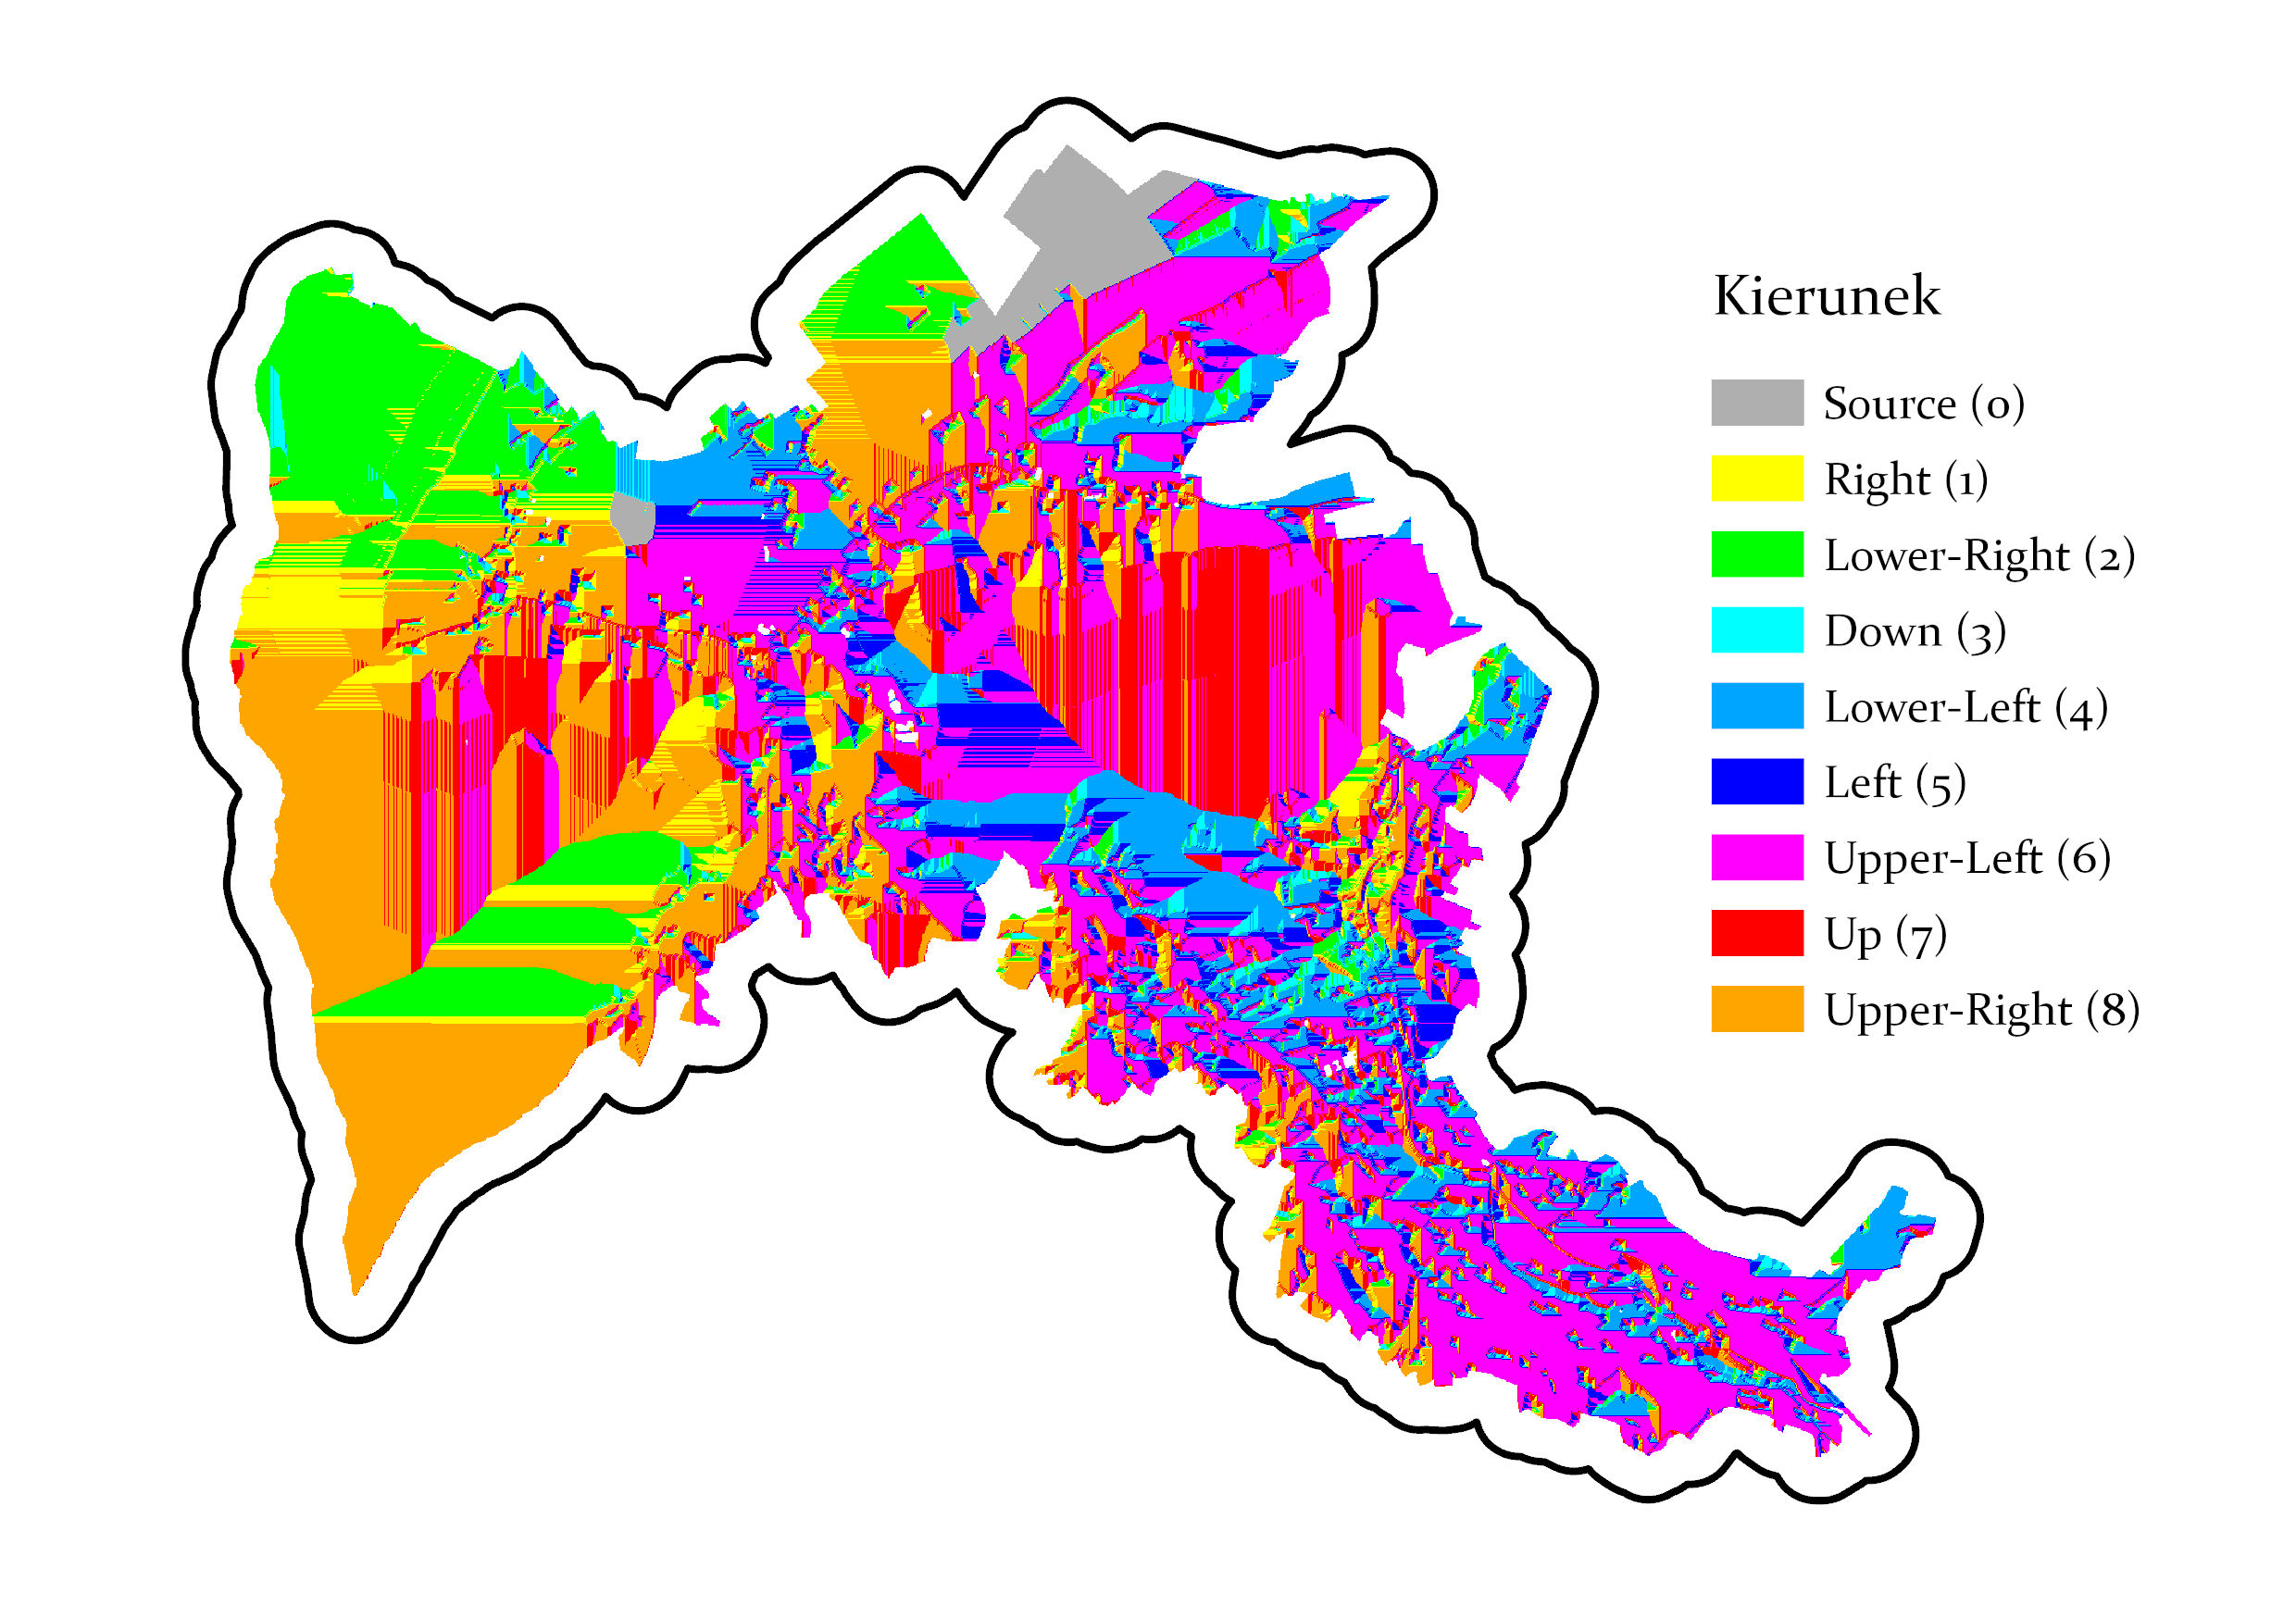
\includegraphics[width=\linewidth]{img/cost-backlink.jpg}
        \caption{Mapa kierunków (backlink) - równe wagi}
        \label{fig:backlink-rowne}
    \end{minipage}
    \hfill
    \begin{minipage}[t]{0.48\textwidth}
        \centering
        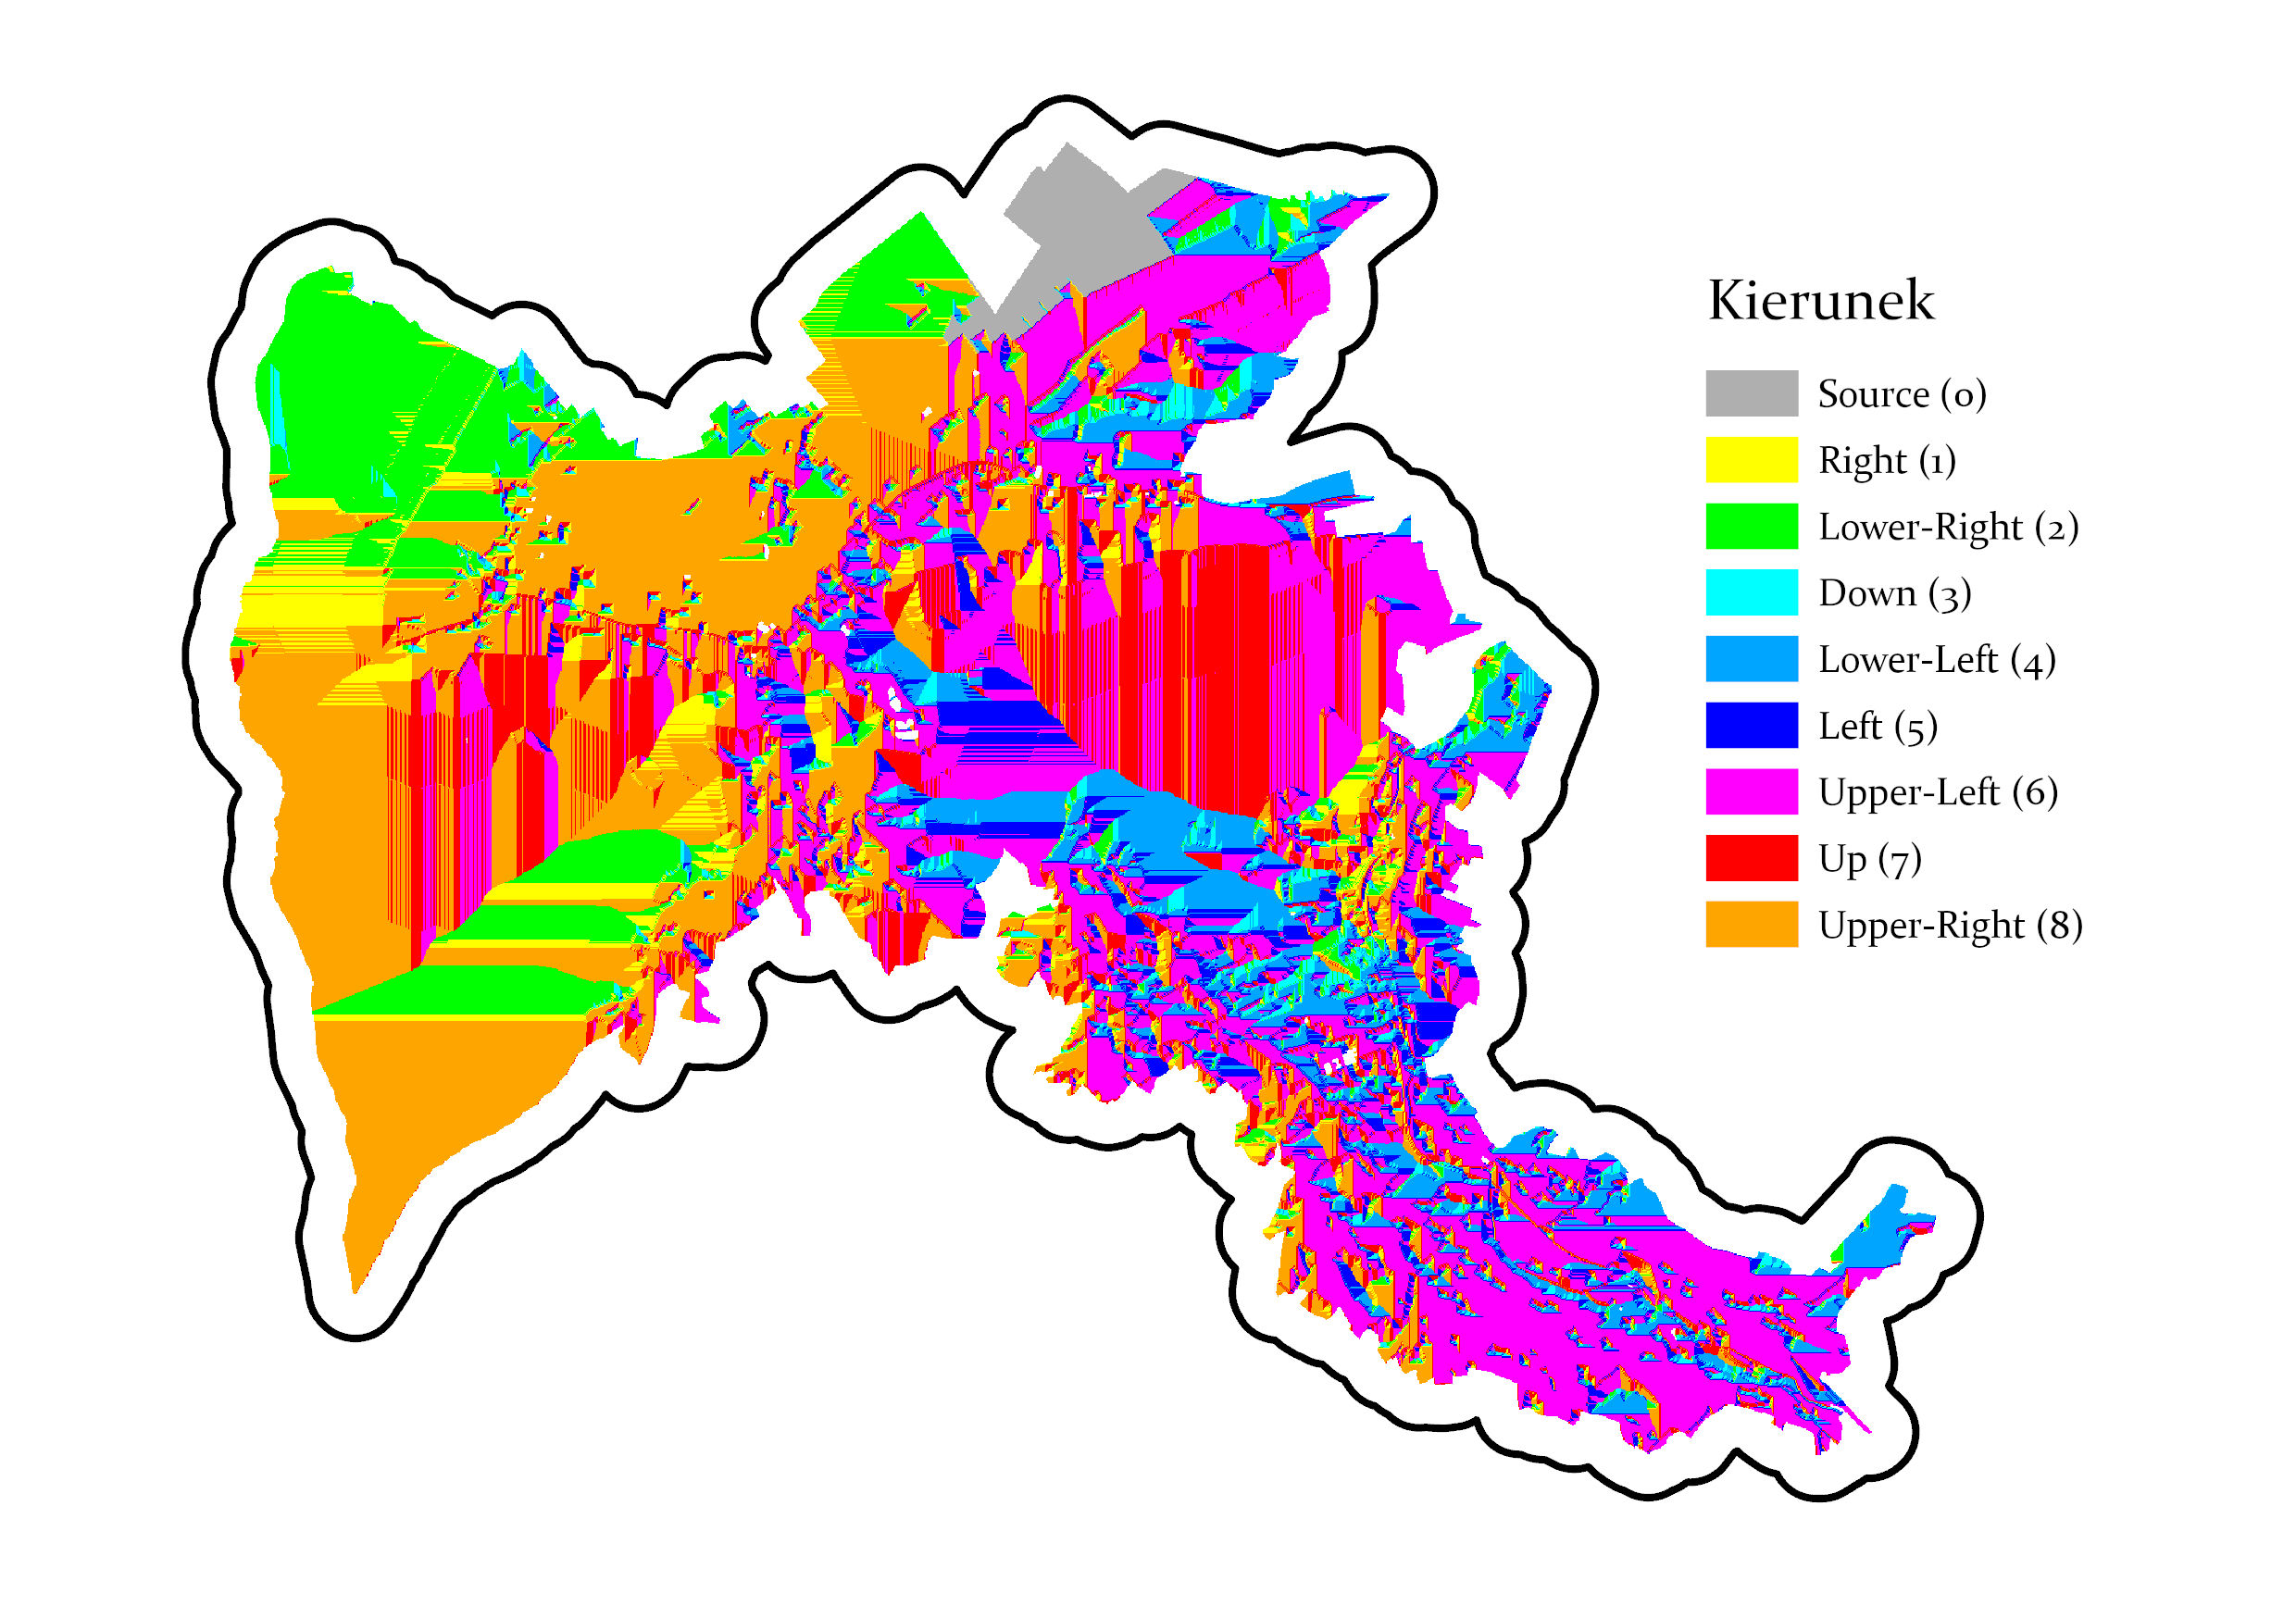
\includegraphics[width=\linewidth]{img/roznewagi-cost-backlink.jpg}
        \caption{Mapa kierunków (backlink) - różne wagi}
        \label{fig:backlink-rozne}
    \end{minipage}
\end{figure}


\begin{figure}[H]
    \begin{minipage}[t]{0.48\textwidth}
        \centering
        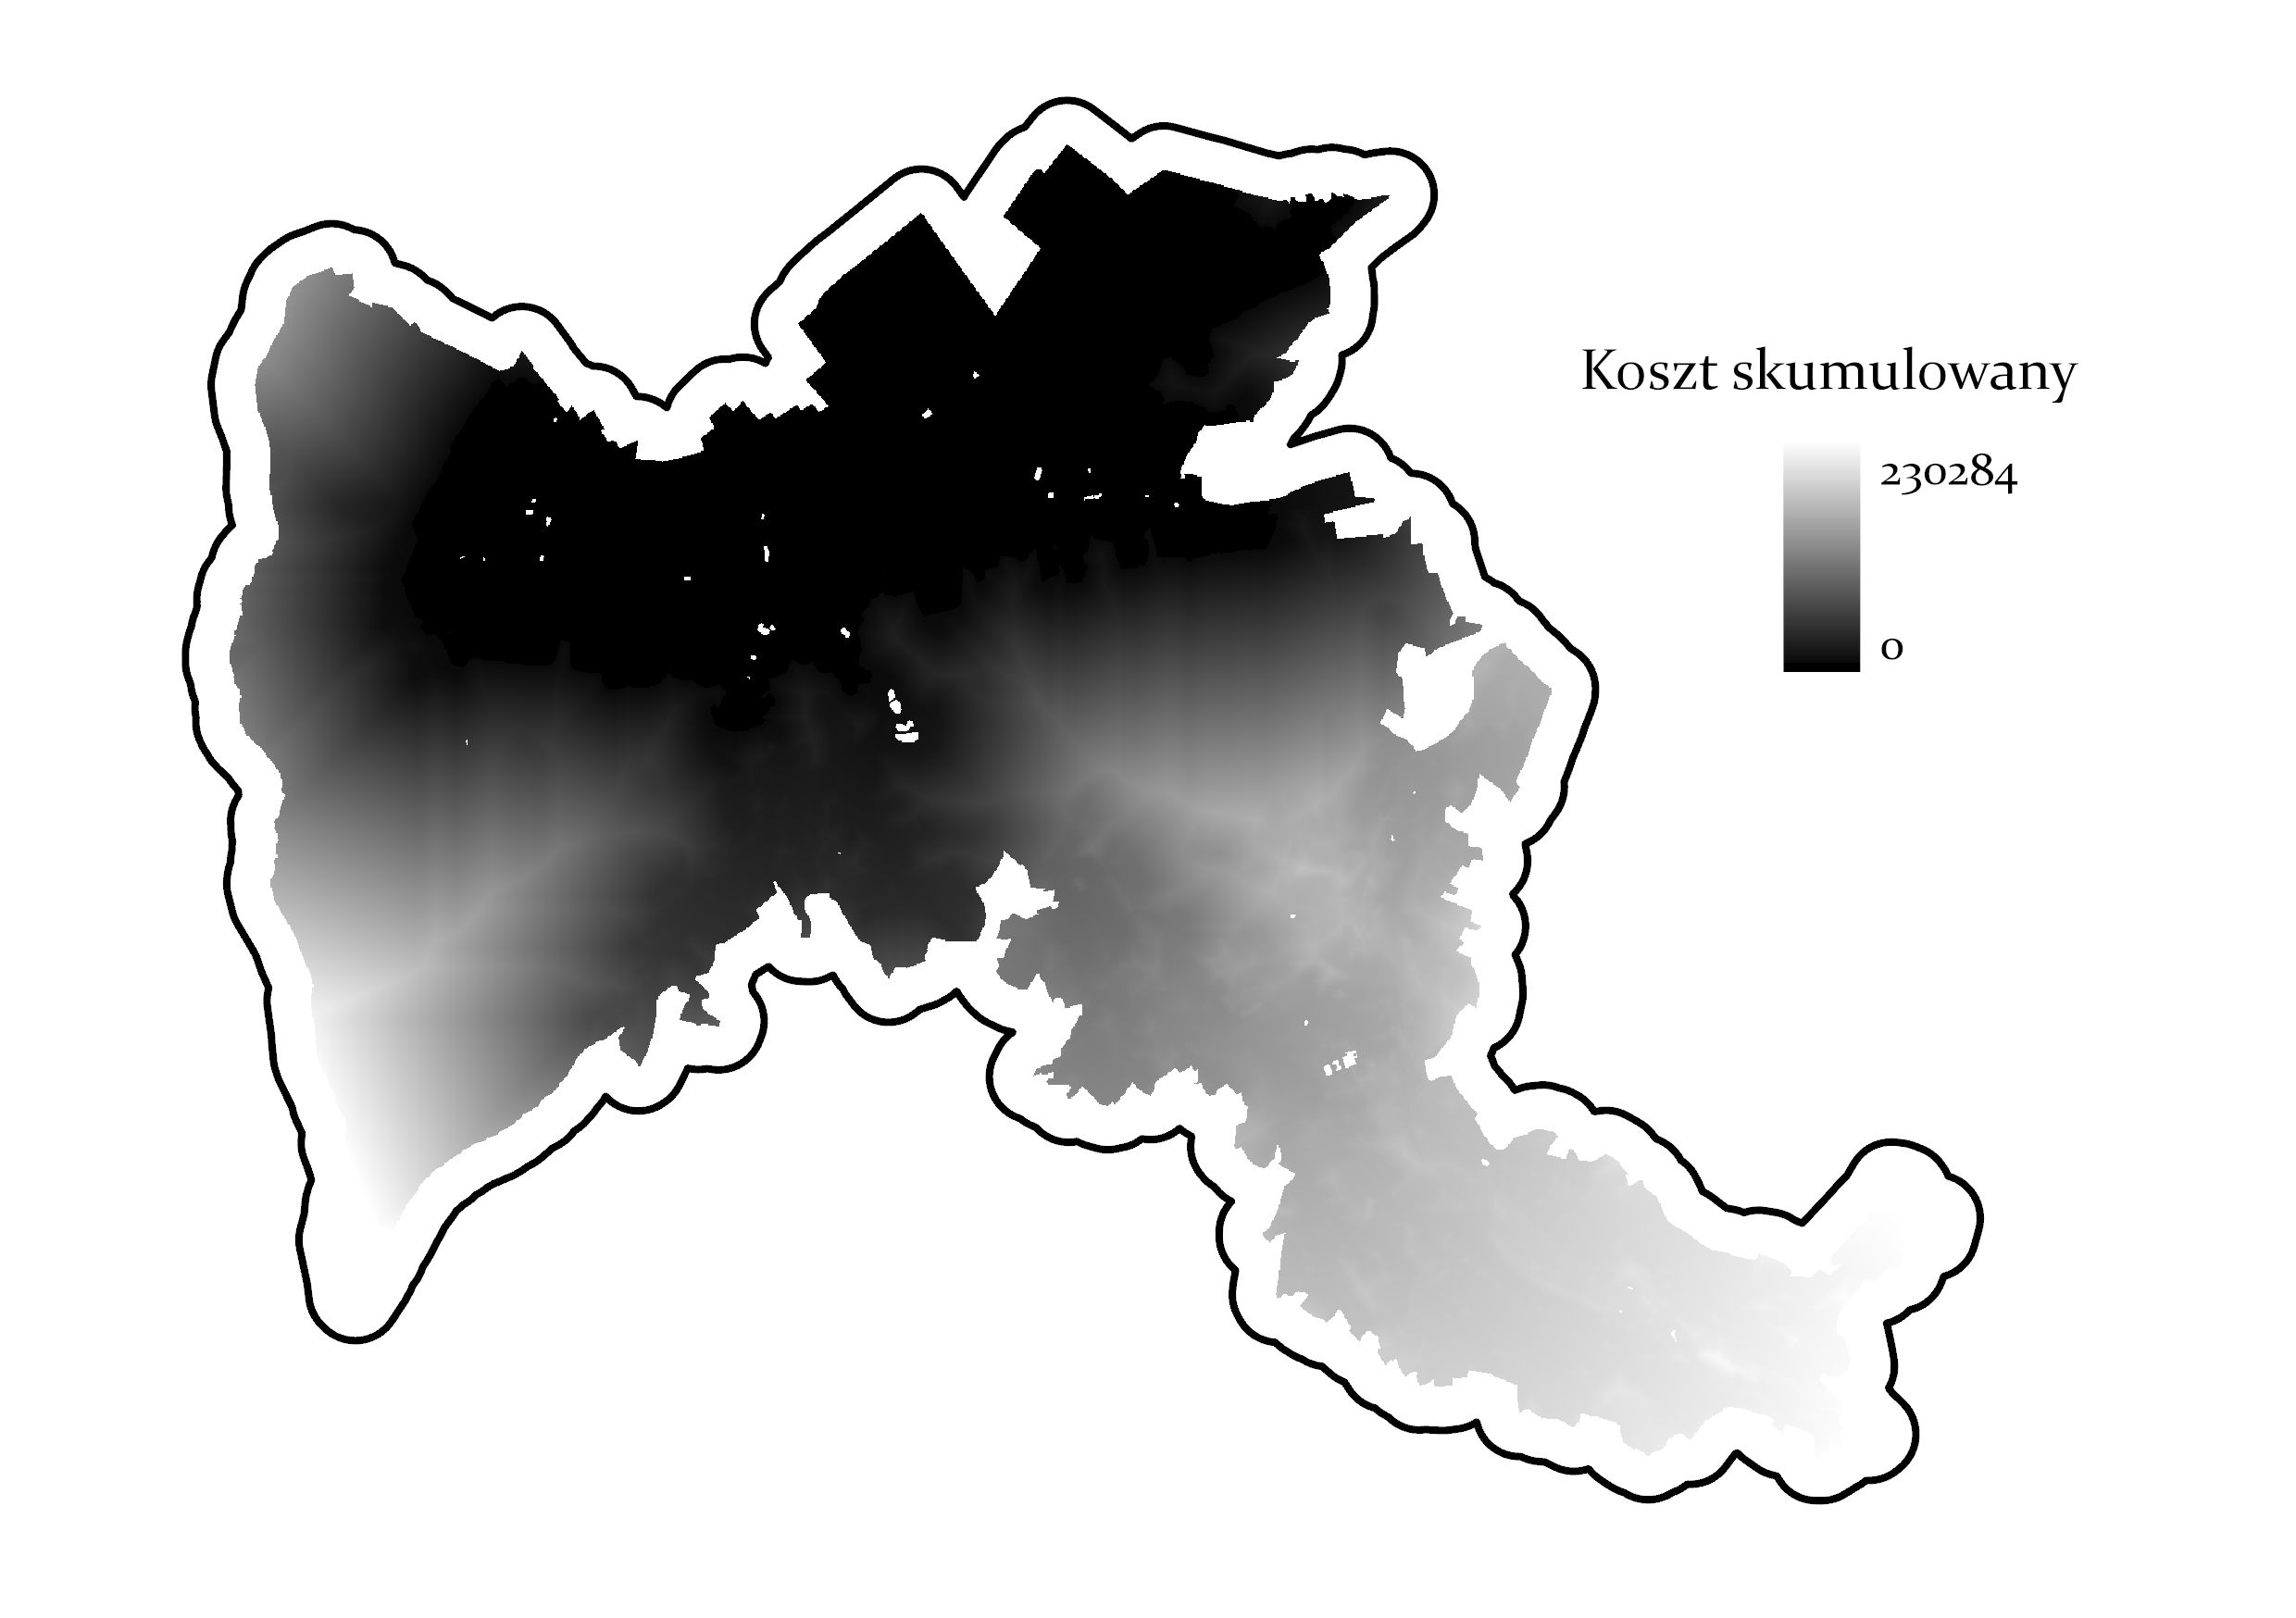
\includegraphics[width=\linewidth]{img/cost-distance.jpg}
        \caption{Mapa kosztów skumulowanych - równe wagi}
        \label{fig:cost-distance-rowne}
    \end{minipage}
    \hfill
    \begin{minipage}[t]{0.48\textwidth}
        \centering
        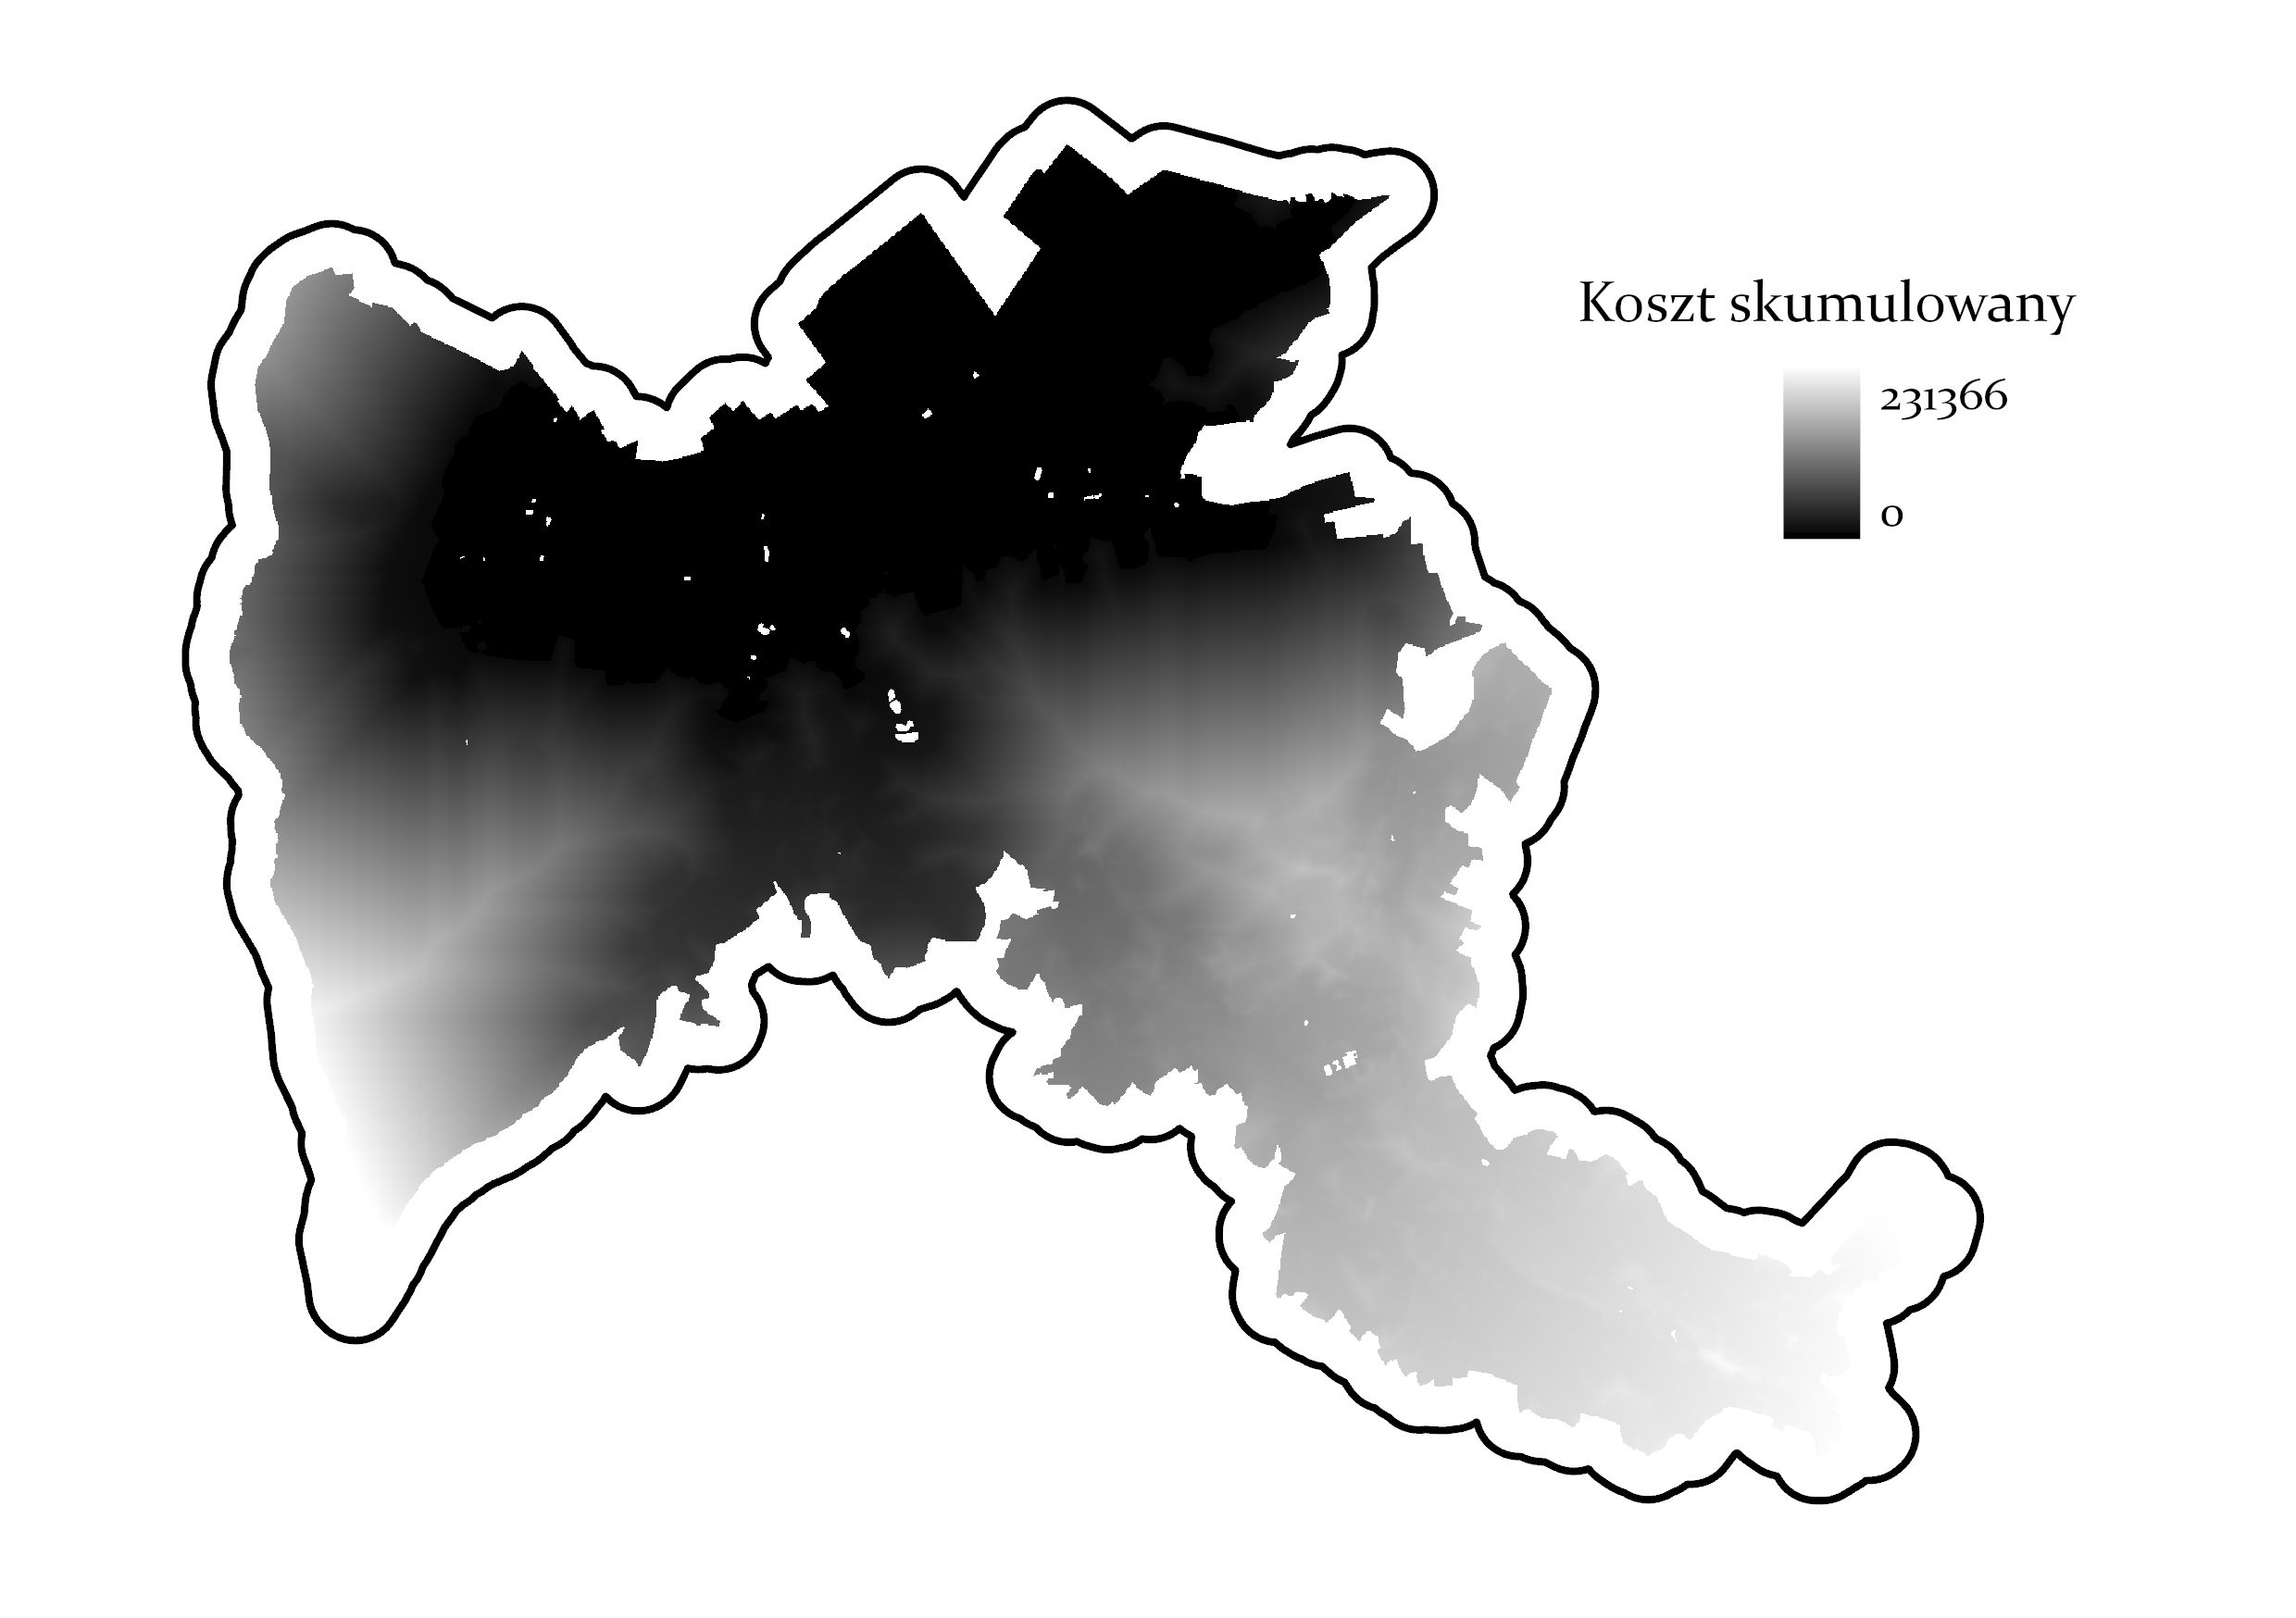
\includegraphics[width=\linewidth]{img/roznewagi-cost-distance.jpg}
        \caption{Mapa kosztów skumulowanych - różne wagi}
        \label{fig:cost-distance-rozne}
    \end{minipage}
\end{figure}


\begin{figure}[H]
    \begin{minipage}[t]{0.48\textwidth}
        \centering
        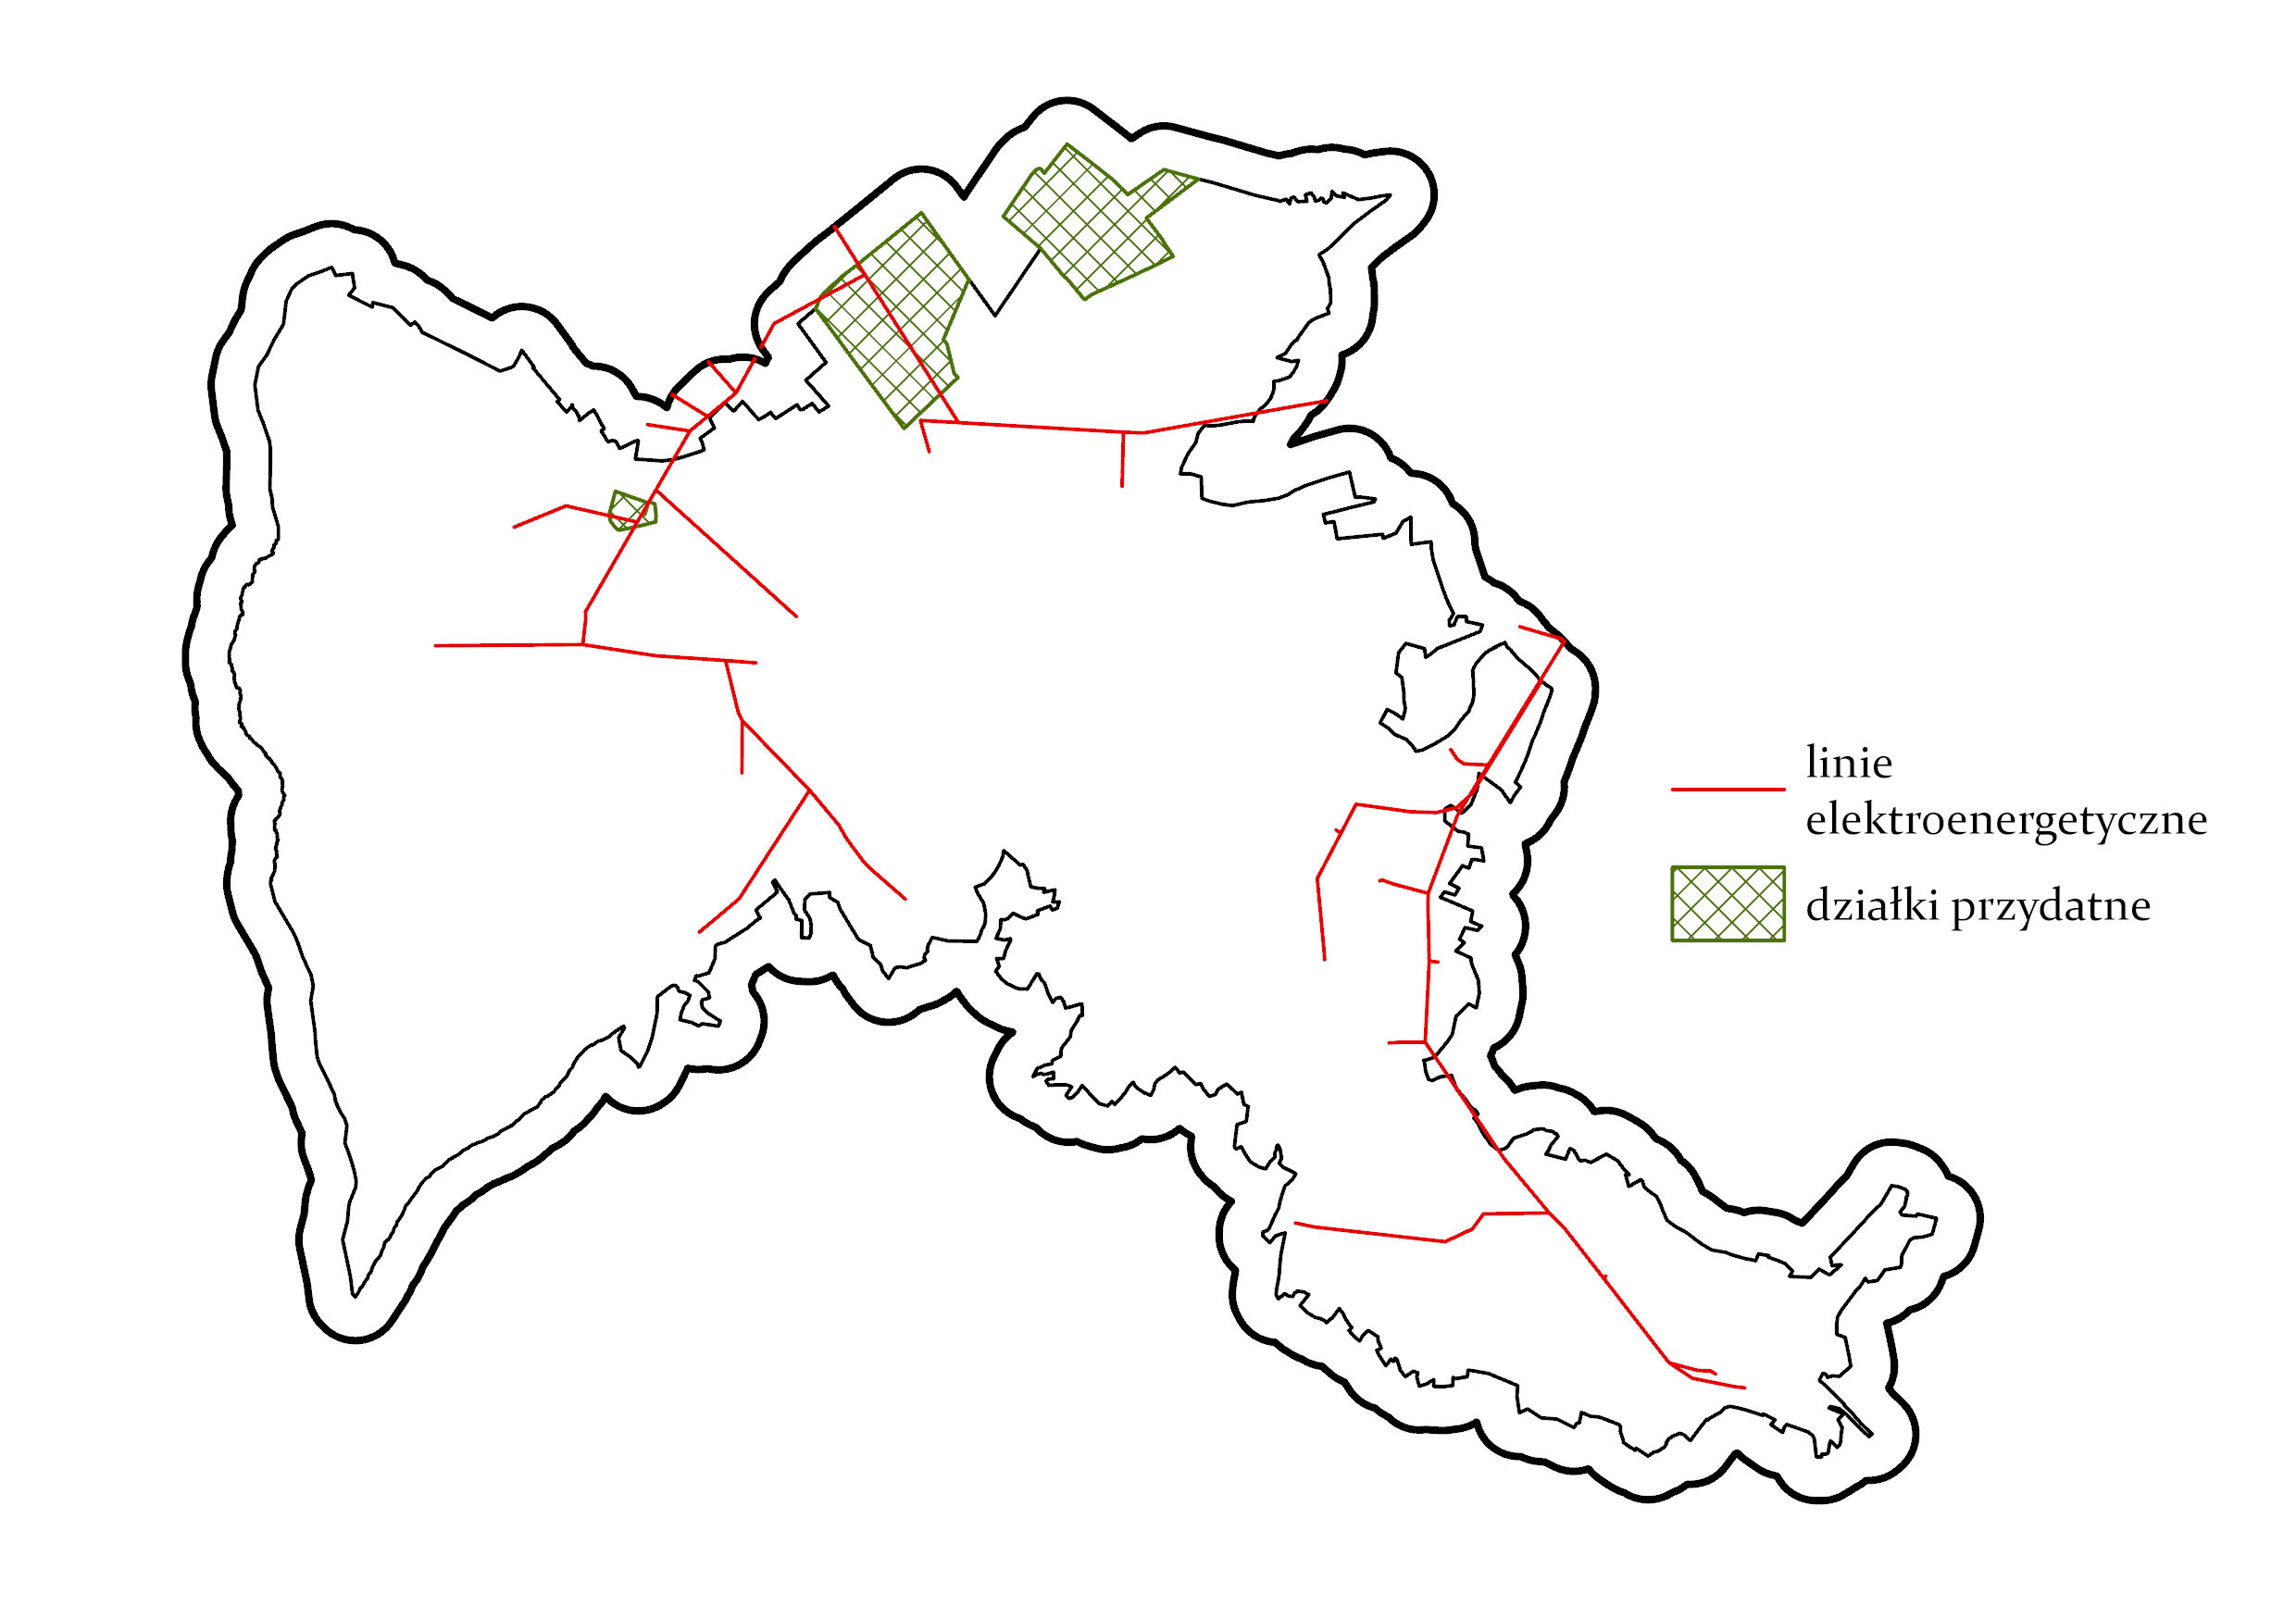
\includegraphics[width=\linewidth]{img/dzialki-linie.jpg}
        \caption{Mapa przedstawiająca przydatne działki oraz linie elektroenergetyczne - równe wagi}
        \label{fig:dzialki-linie-rowne}
    \end{minipage}
    \hfill
    \begin{minipage}[t]{0.48\textwidth}
        \centering
        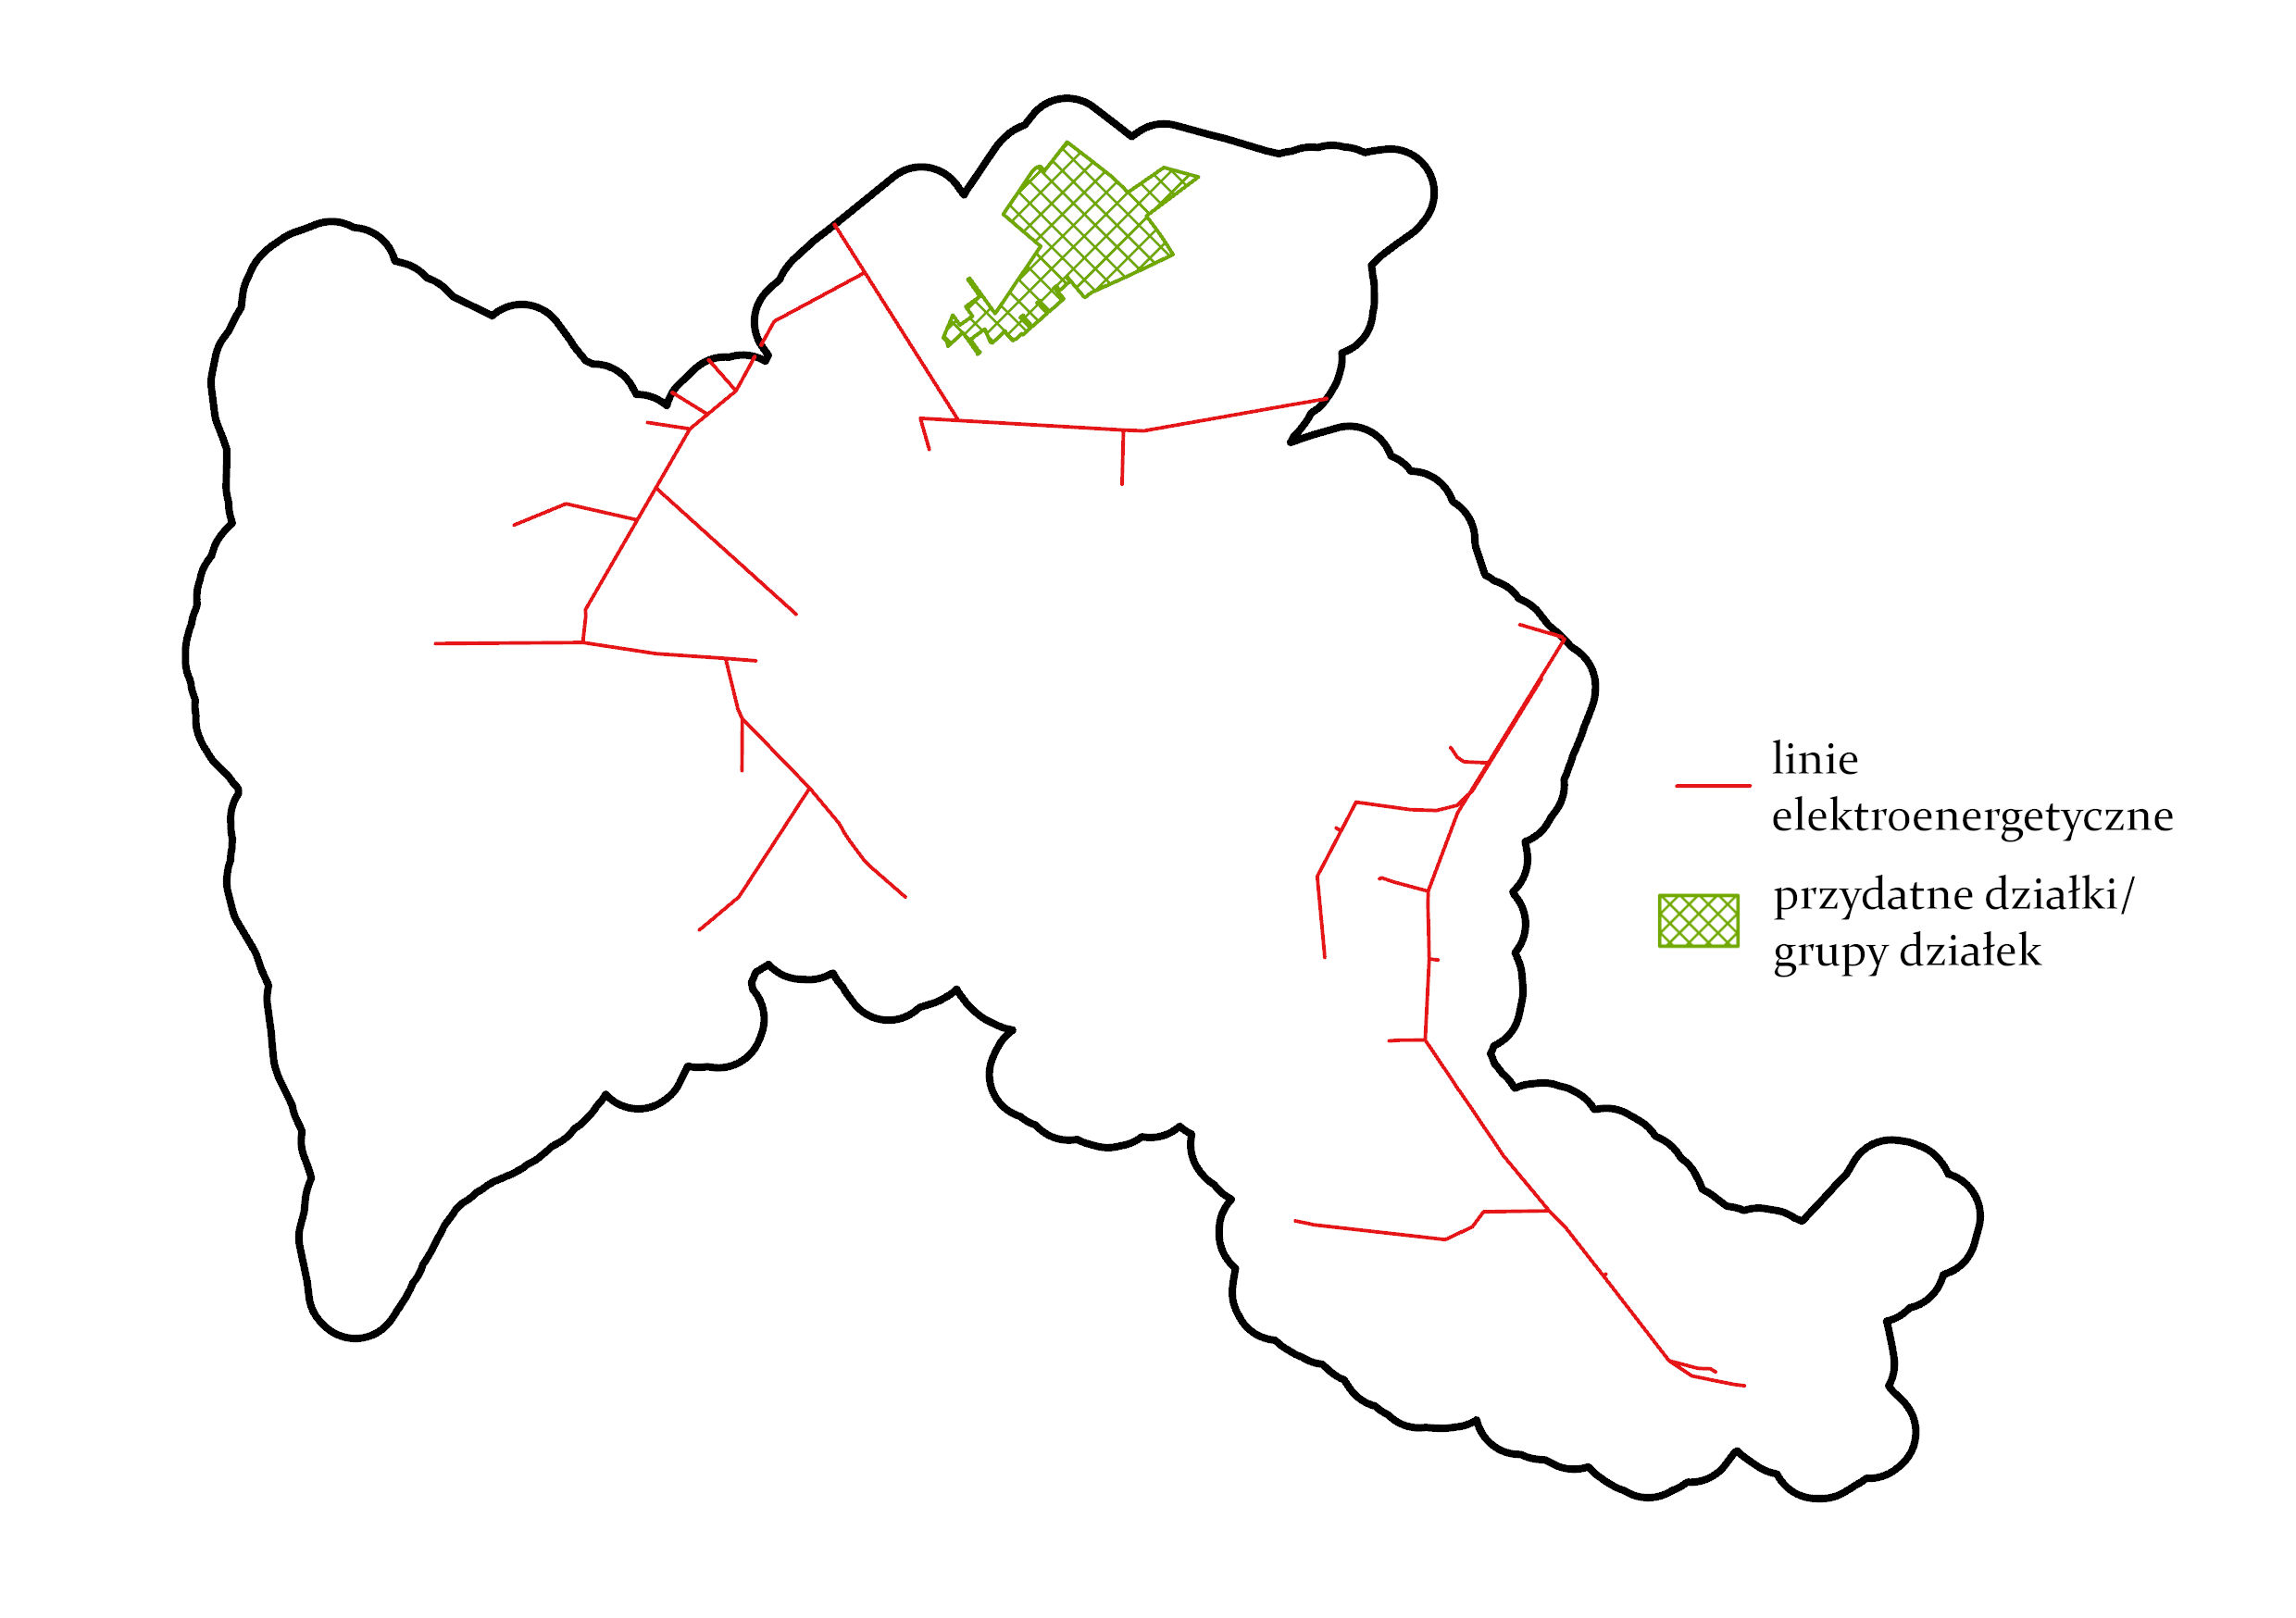
\includegraphics[width=\linewidth]{img/roznewagi-dzialki-linie.jpg}
        \caption{Mapa przedstawiająca przydatne działki oraz linie elektroenergetyczne - różne wagi}
        \label{fig:dzialki-linie-rozne}
    \end{minipage}
\end{figure}

W przypadku wersji z równymi wagami, linia elektroenergetyczna przechodzi przez jedną z wytypowanych grup działek. W związku z tym żadna ścieżka przyłącza nie została utworzona. Poniżej znajduje się wersja przyłącza utworzona dla wersji z różnymi wagami dla kryteriów.

\begin{figure}[H]
    \centering
    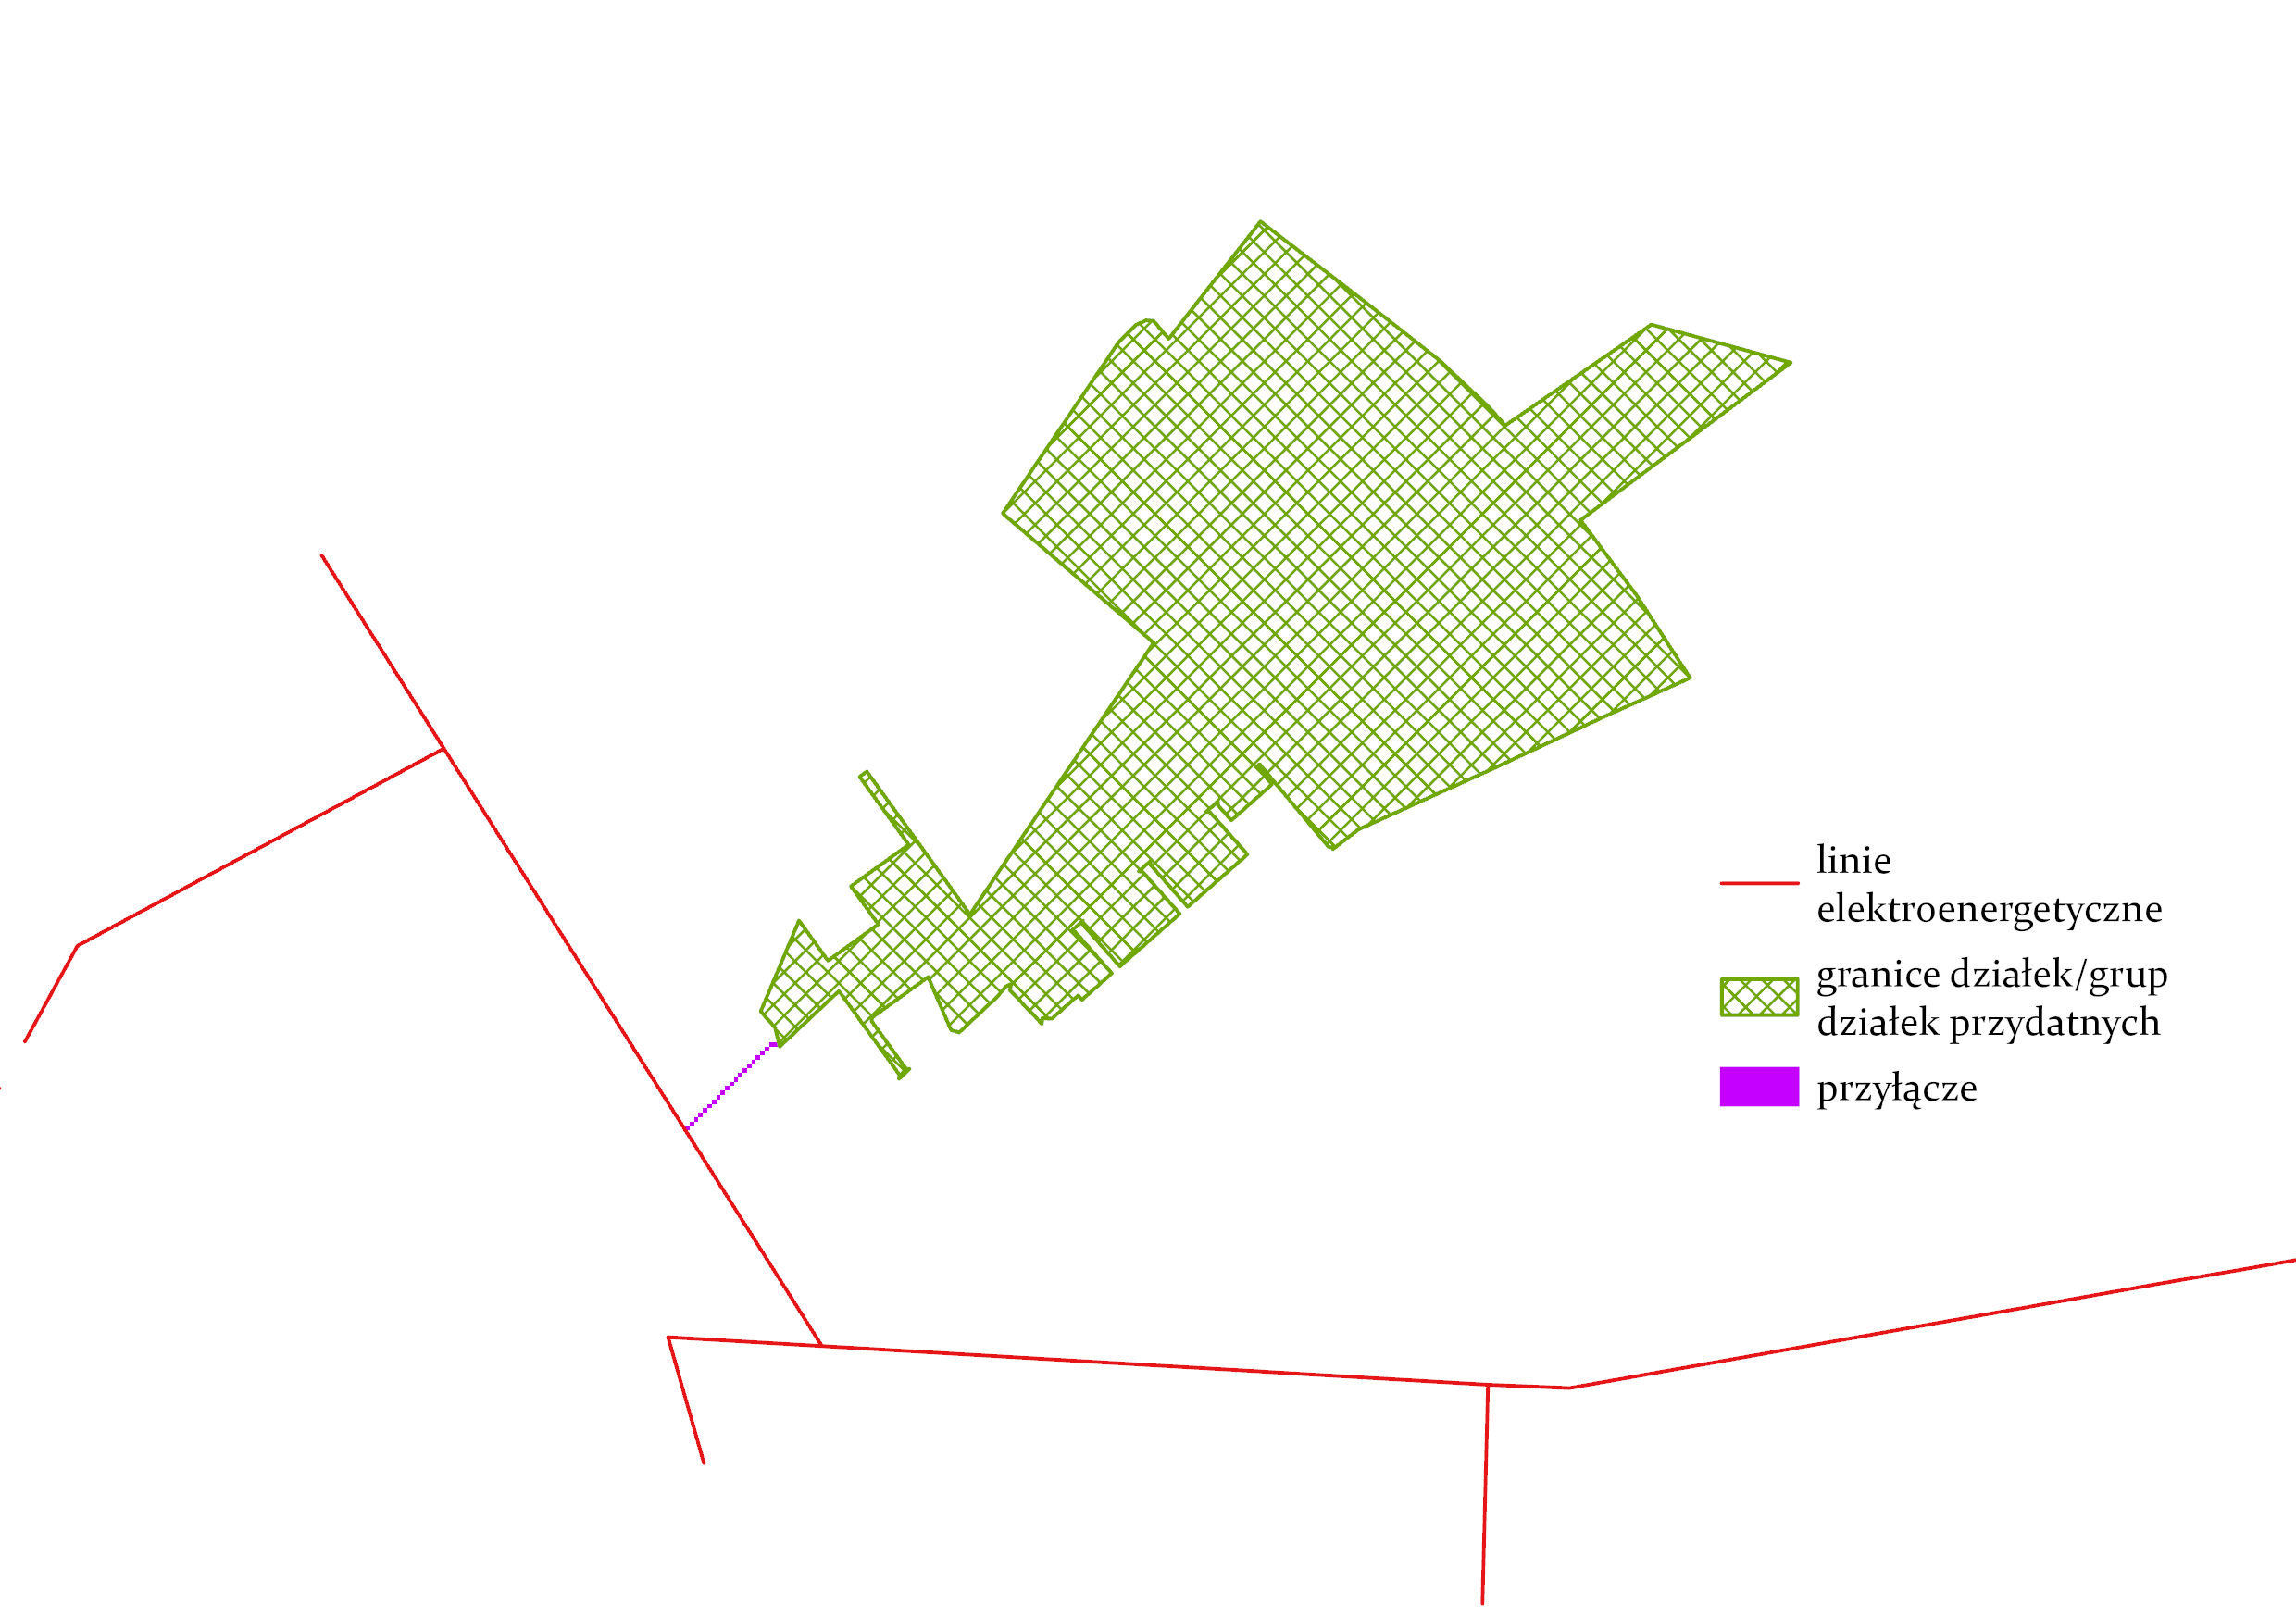
\includegraphics[width=0.65\textwidth]{img/roznewagi-path-raster.jpg}
    \caption{Mapa przedstawiająca utworzoną ścieżkę w postaci rastrowej - różne wagi}
\end{figure}

\begin{figure}[H]
    \centering
    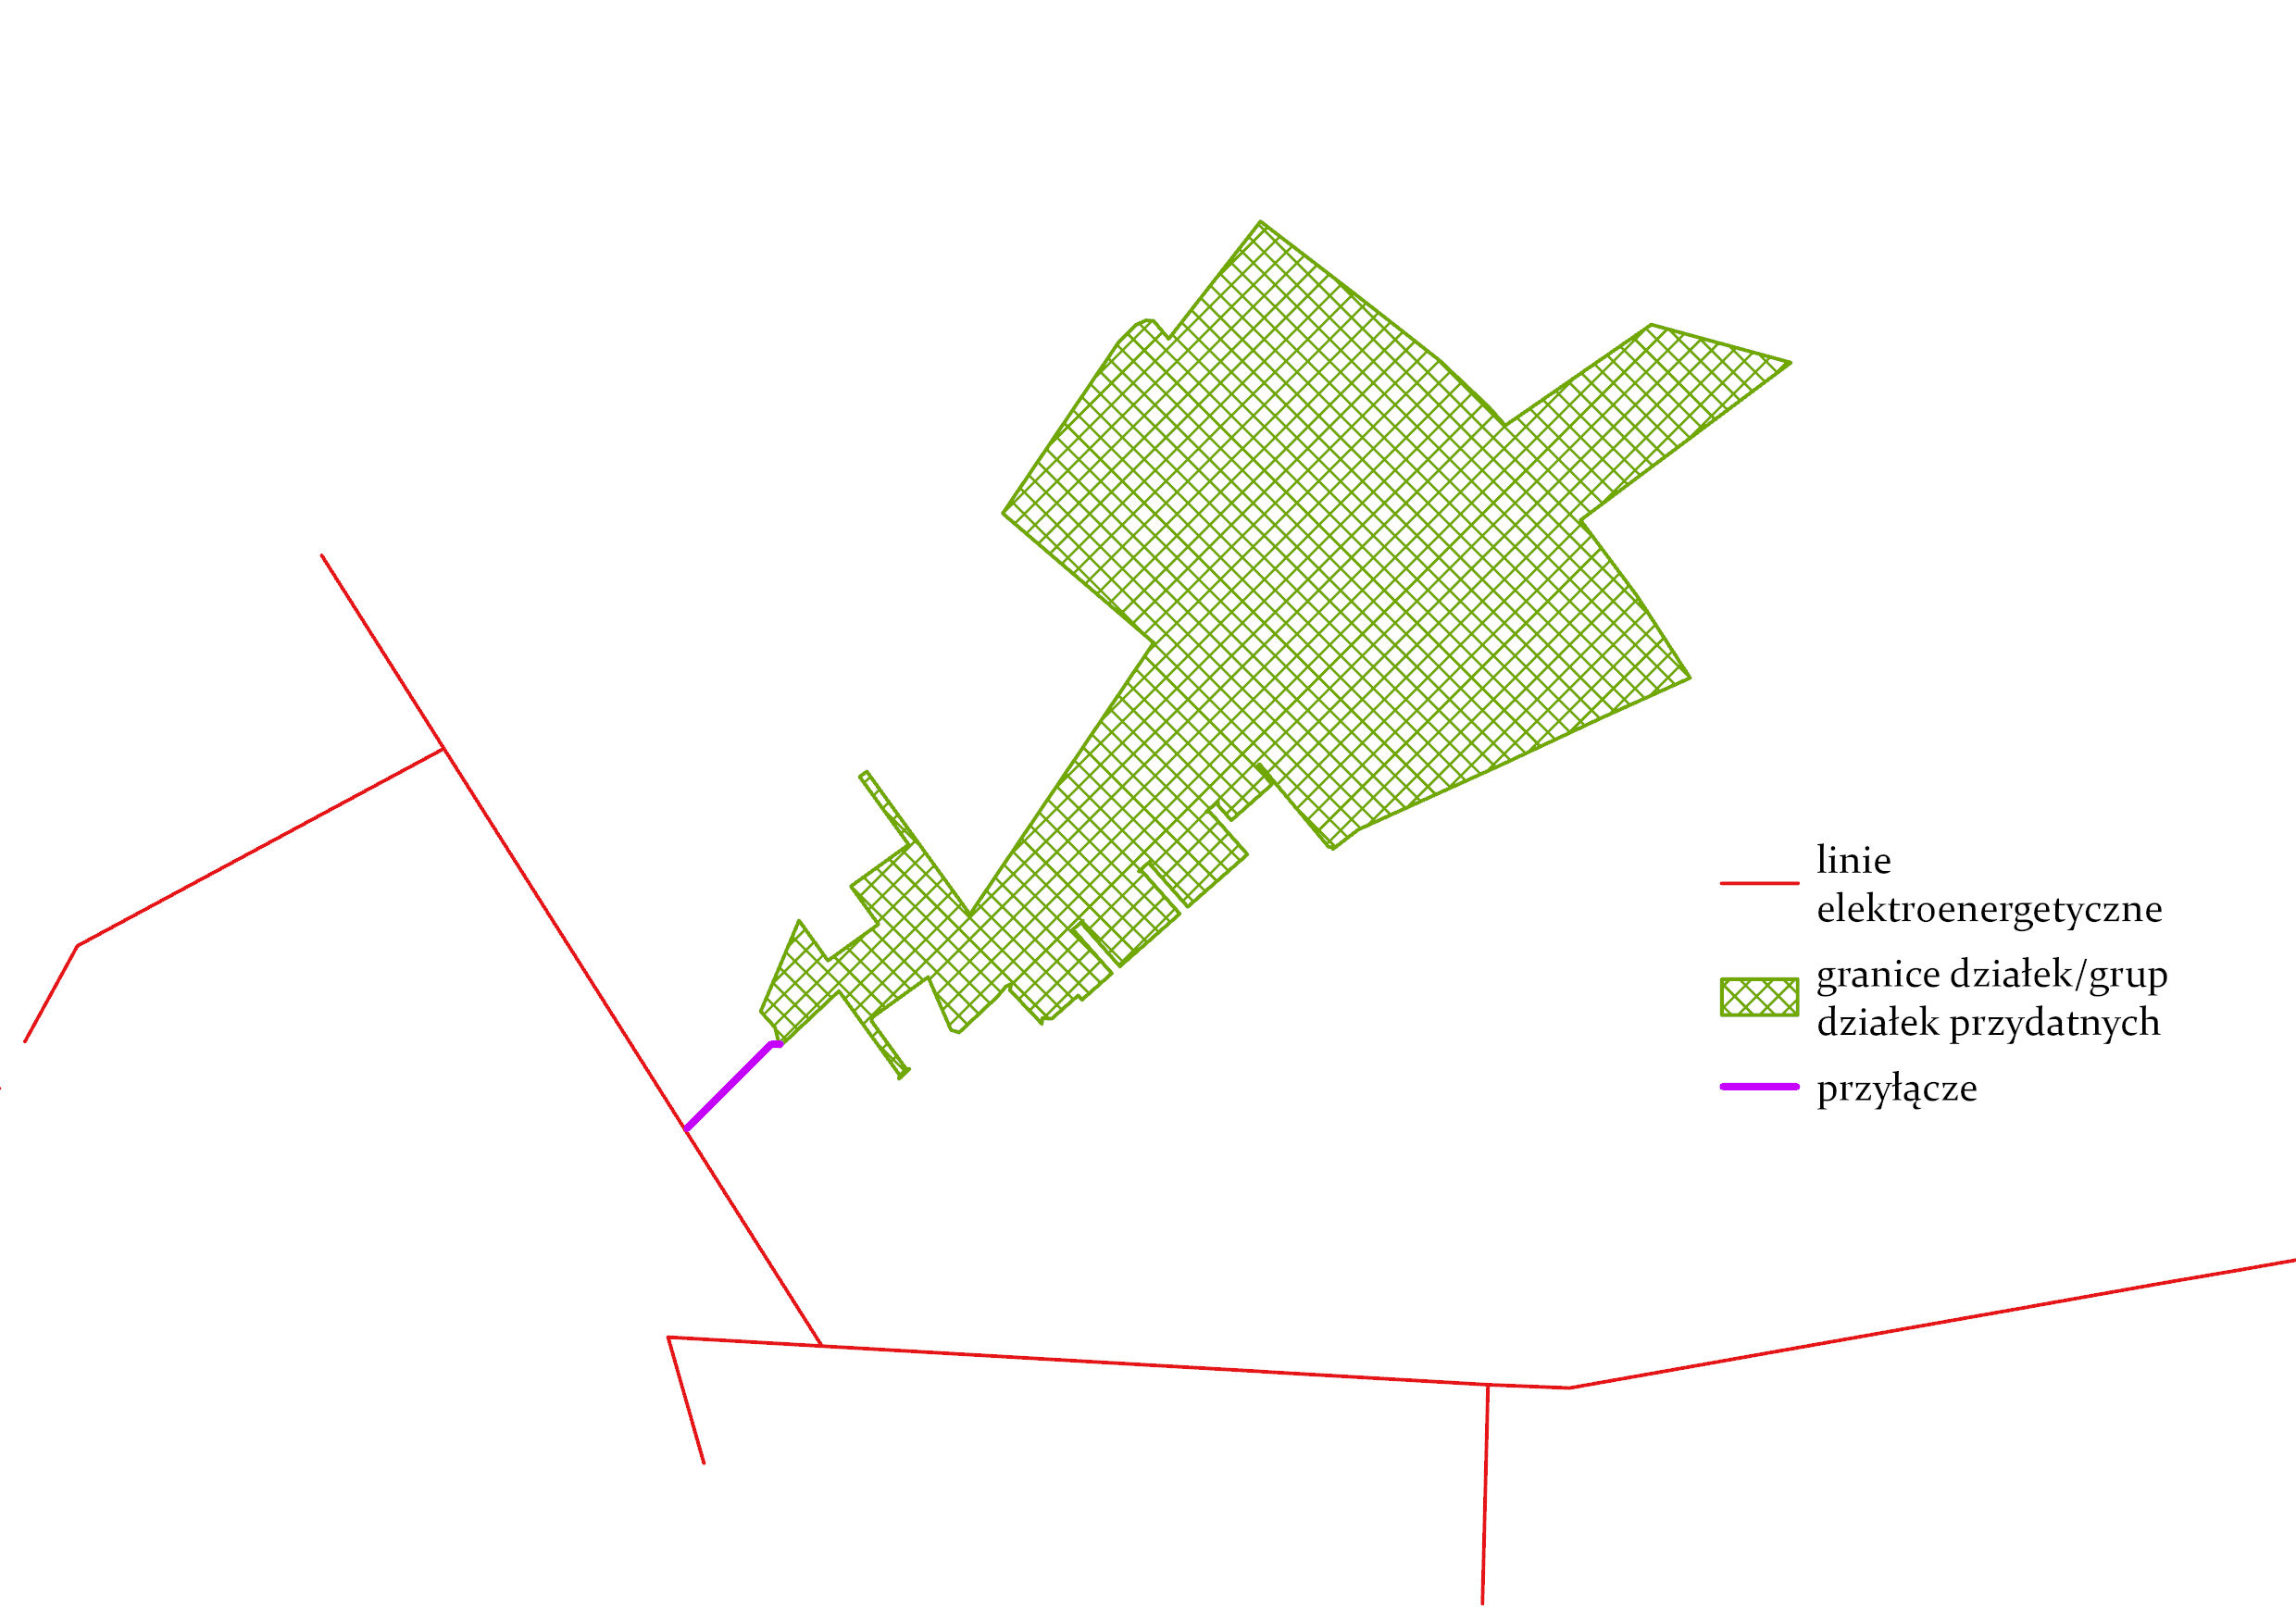
\includegraphics[width=0.65\textwidth]{img/roznewagi-path-vector.jpg}
    \caption{Mapa przedstawiająca utworzoną ścieżkę w postaci wektorowej - różne wagi}
\end{figure}
\newpage

\section{Test modelu na danych z innego obszaru}
\subsection{Opis obszaru}
Stworzony model należało przetestować na innym obszarze. Wybrano do tego celu gminę Pleśna - wiejską gminę w powiecie tarnowskim w województwie małopolskim.

\begin{figure}[H]
    \centering
    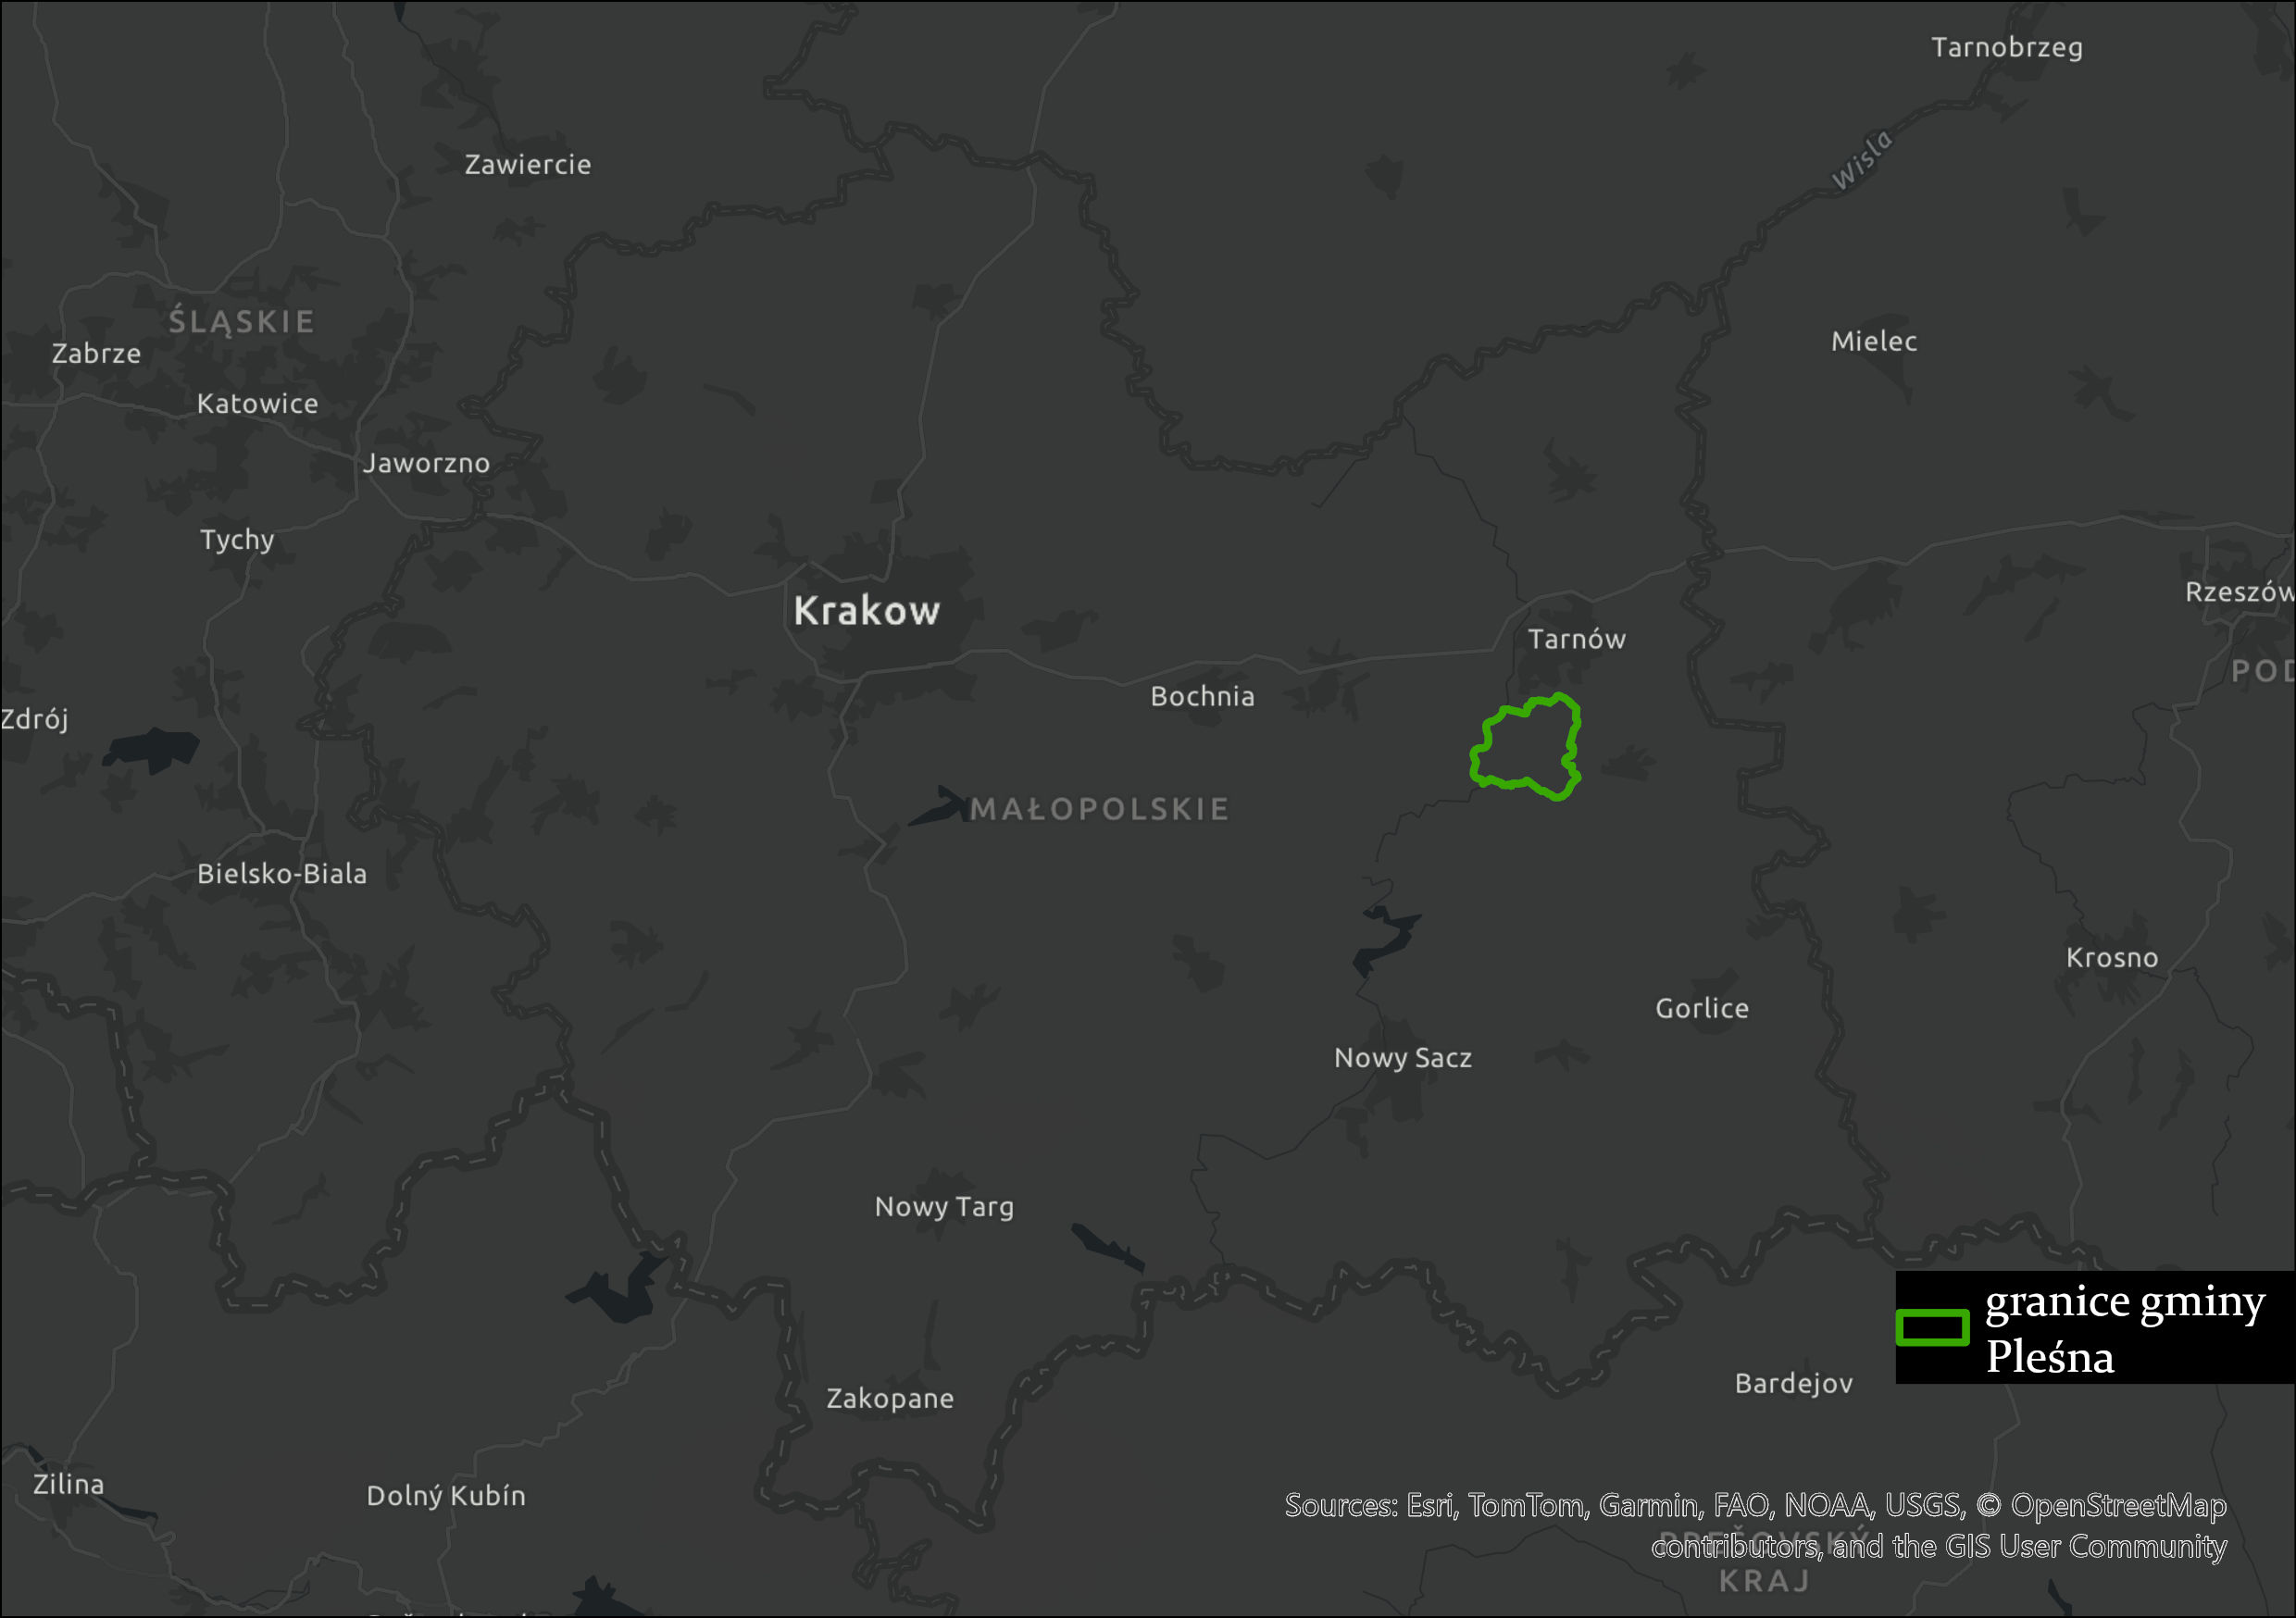
\includegraphics[width=0.75\textwidth]{img/plesna-polozenie.jpg}
    \caption{Położenie gminy na mapie województwa małopolskiego}
\end{figure}

\subsection{Kryterium 1: odległość od rzek i zbiorników wodnych}
W gminie występuje duża gęstość rzek i zbiorników wodnych, lecz ze względu na łagodnie postawione granice dla tego kryterium, duża część obszaru gminy cechuje się dużą przydatnością.

\begin{figure}[H]
    \centering
    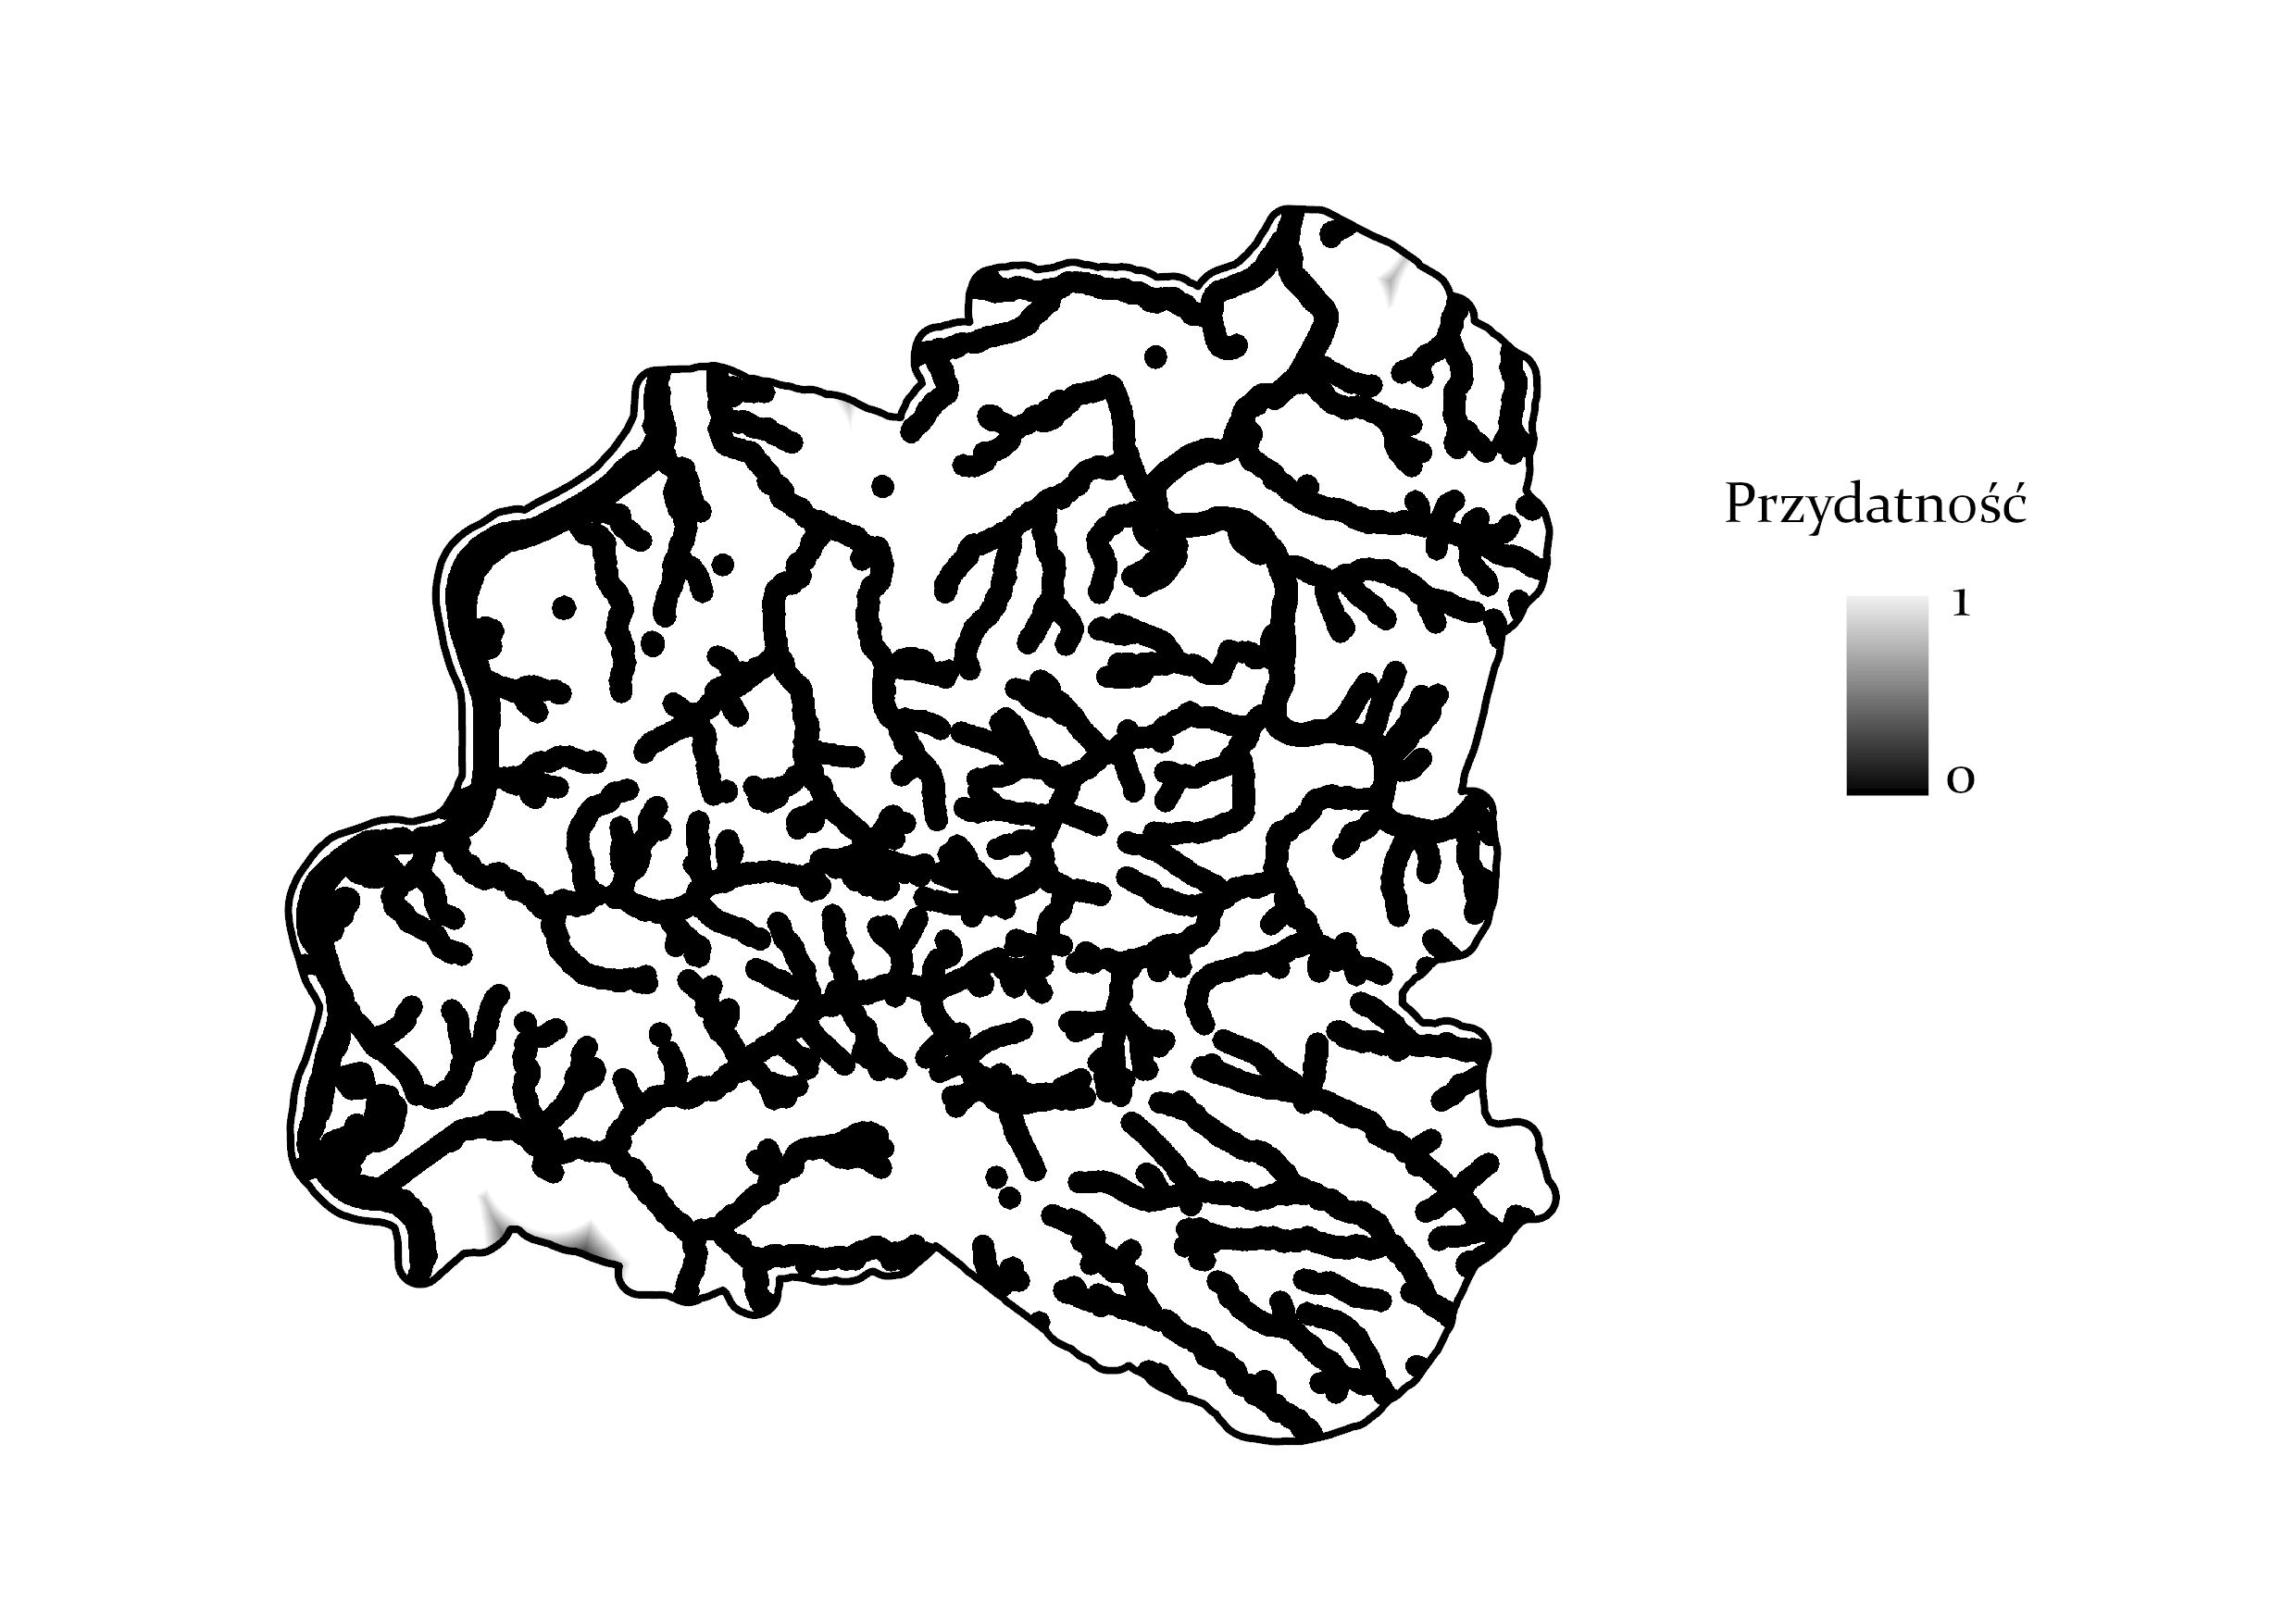
\includegraphics[width=0.75\textwidth]{img/plesna-kryterium1-layout.jpg}
    \caption{Mapa przydatności dla kryterium 1.}
\end{figure}

\begin{figure}[H]
    \centering
    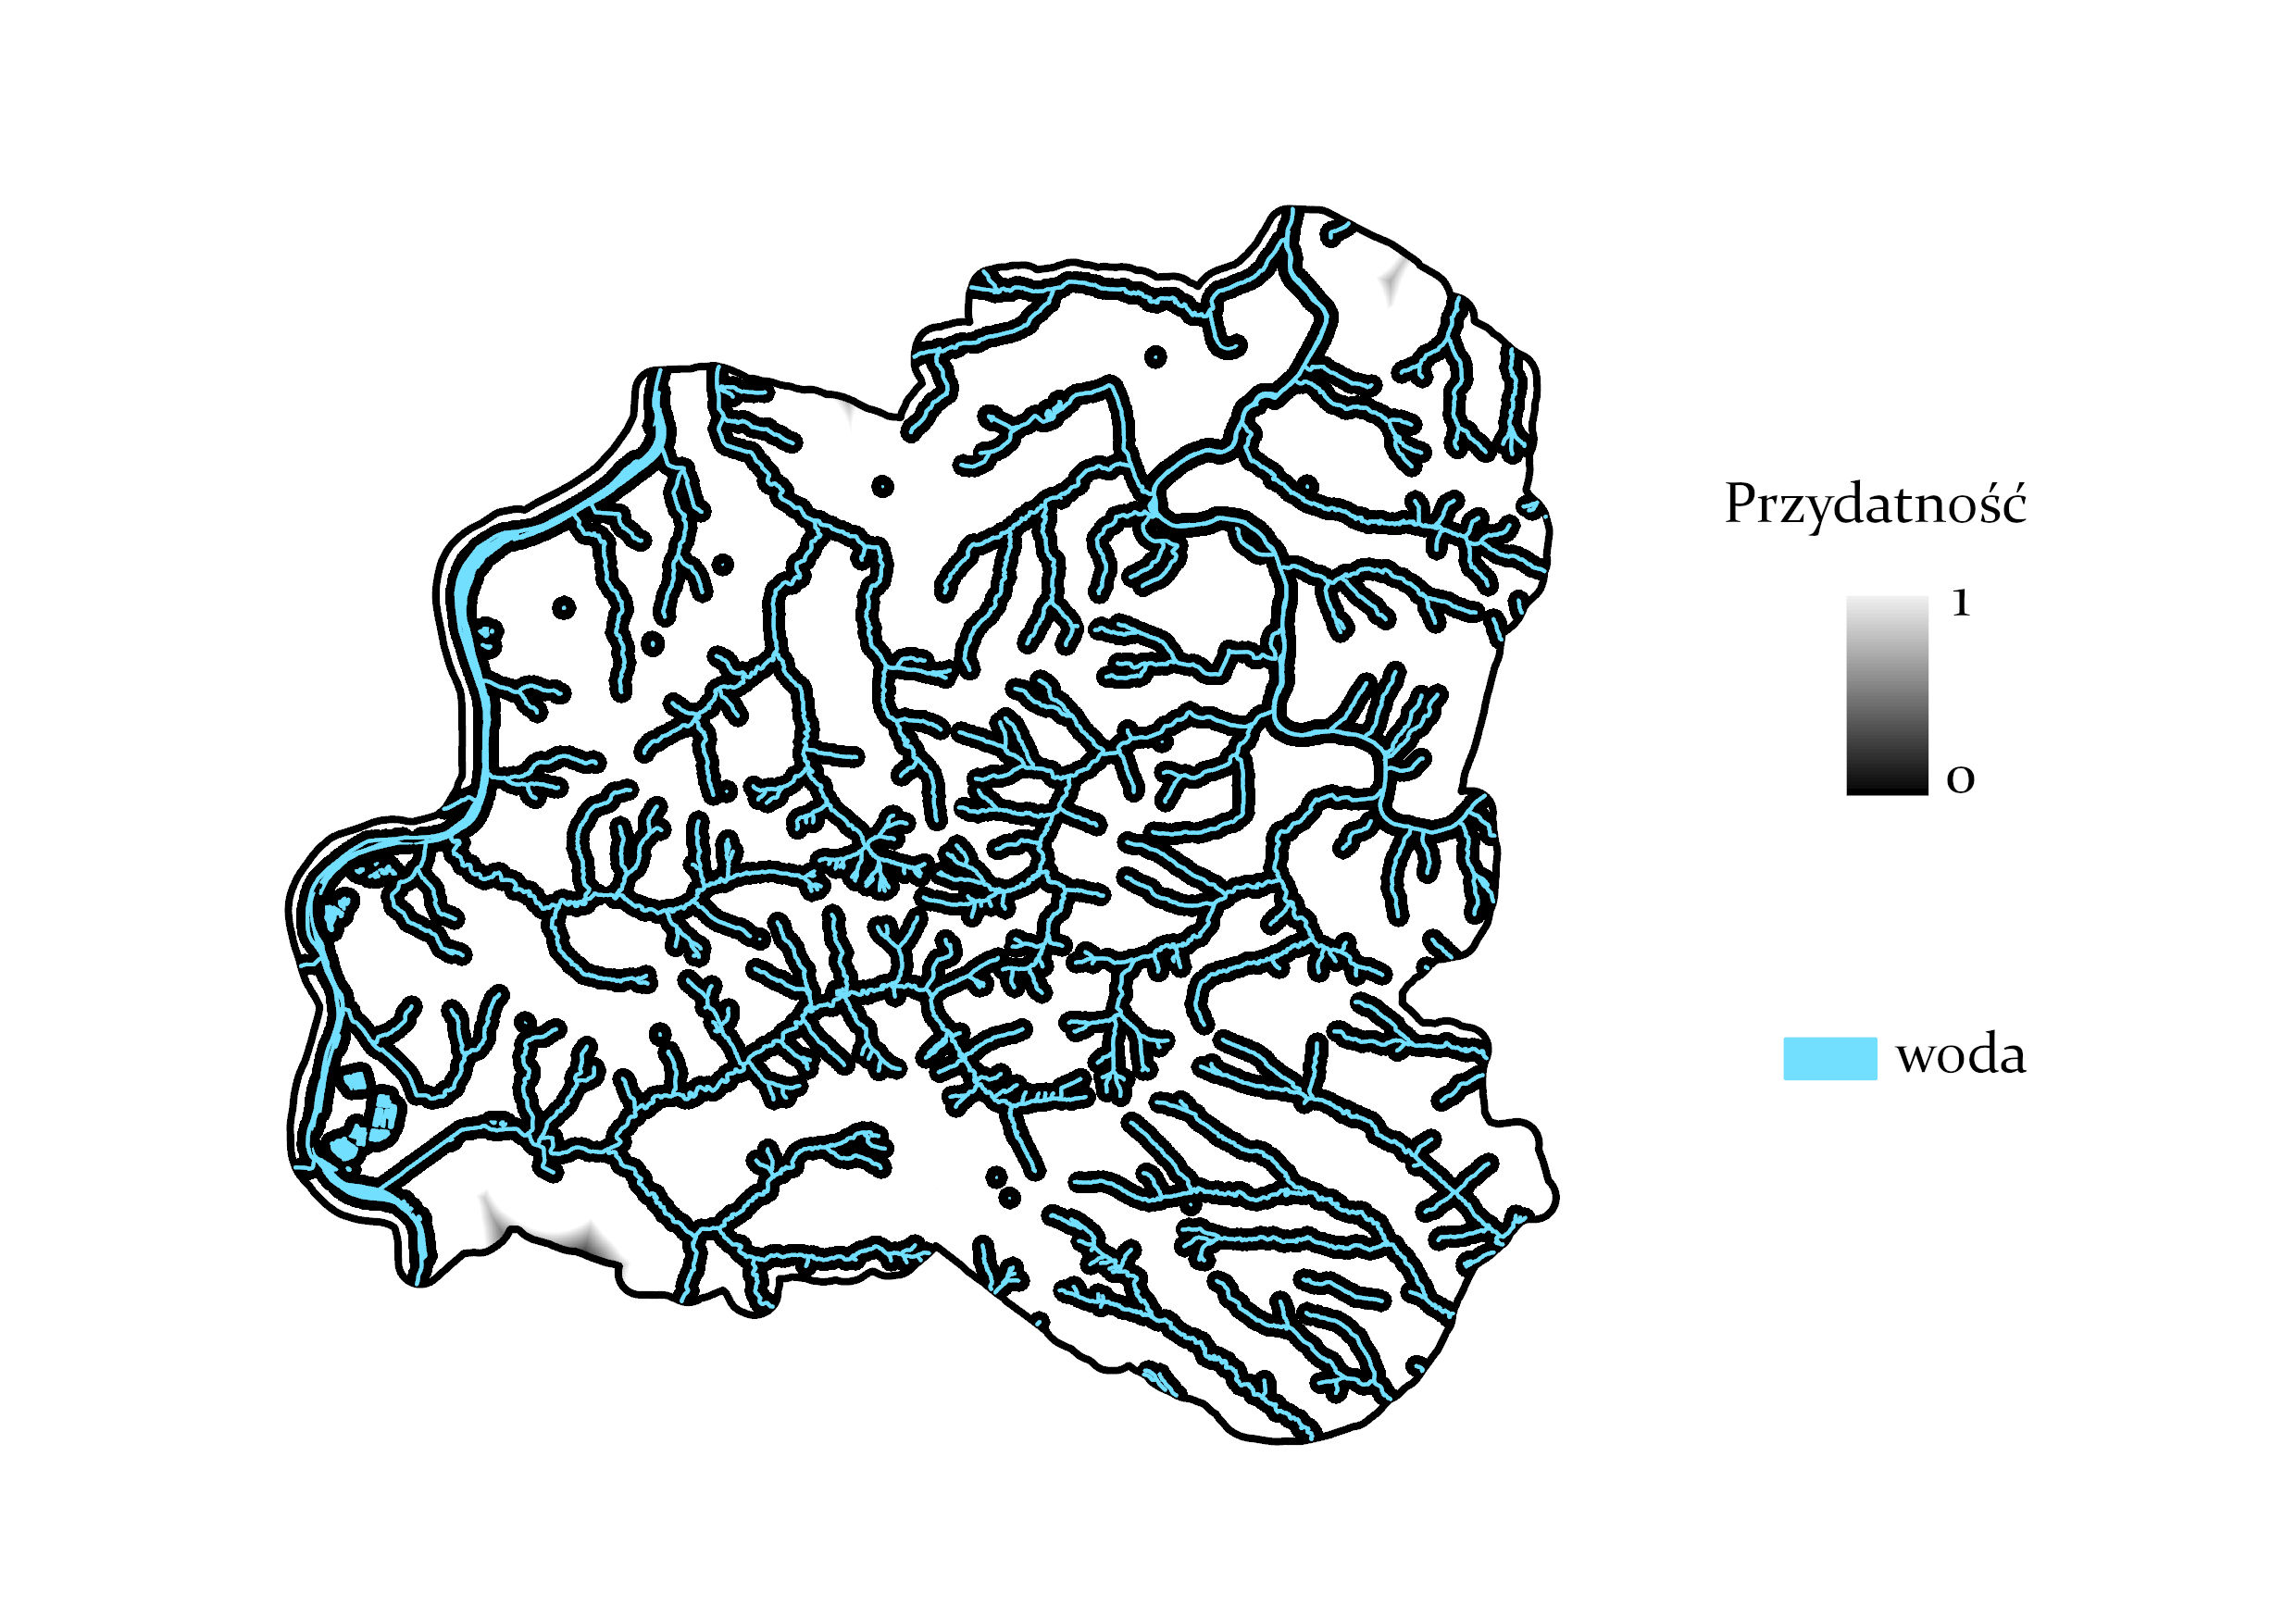
\includegraphics[width=0.75\textwidth]{img/plesna-kryterium1-woda.jpg}
    \caption{Mapa przydatności dla kryterium 1. zawierająca rzeki oraz zbiorniki wodne}
\end{figure}

\subsection{Kryterium 2: odległość od budynków mieszkalnych}
Jak widać poniżej, w gminie znajduje się wiele budynków mieszkalnych, rozmieszczonych mniej więcj równomiernie po całym jej obszarze. Duża część terenu zostaje już na tym etapie wyeliminowana ze względu na obecność kryterium ostrego odległości powyżej 150 metrów od budynków mieszkalnych.

\begin{figure}[H]
    \centering
    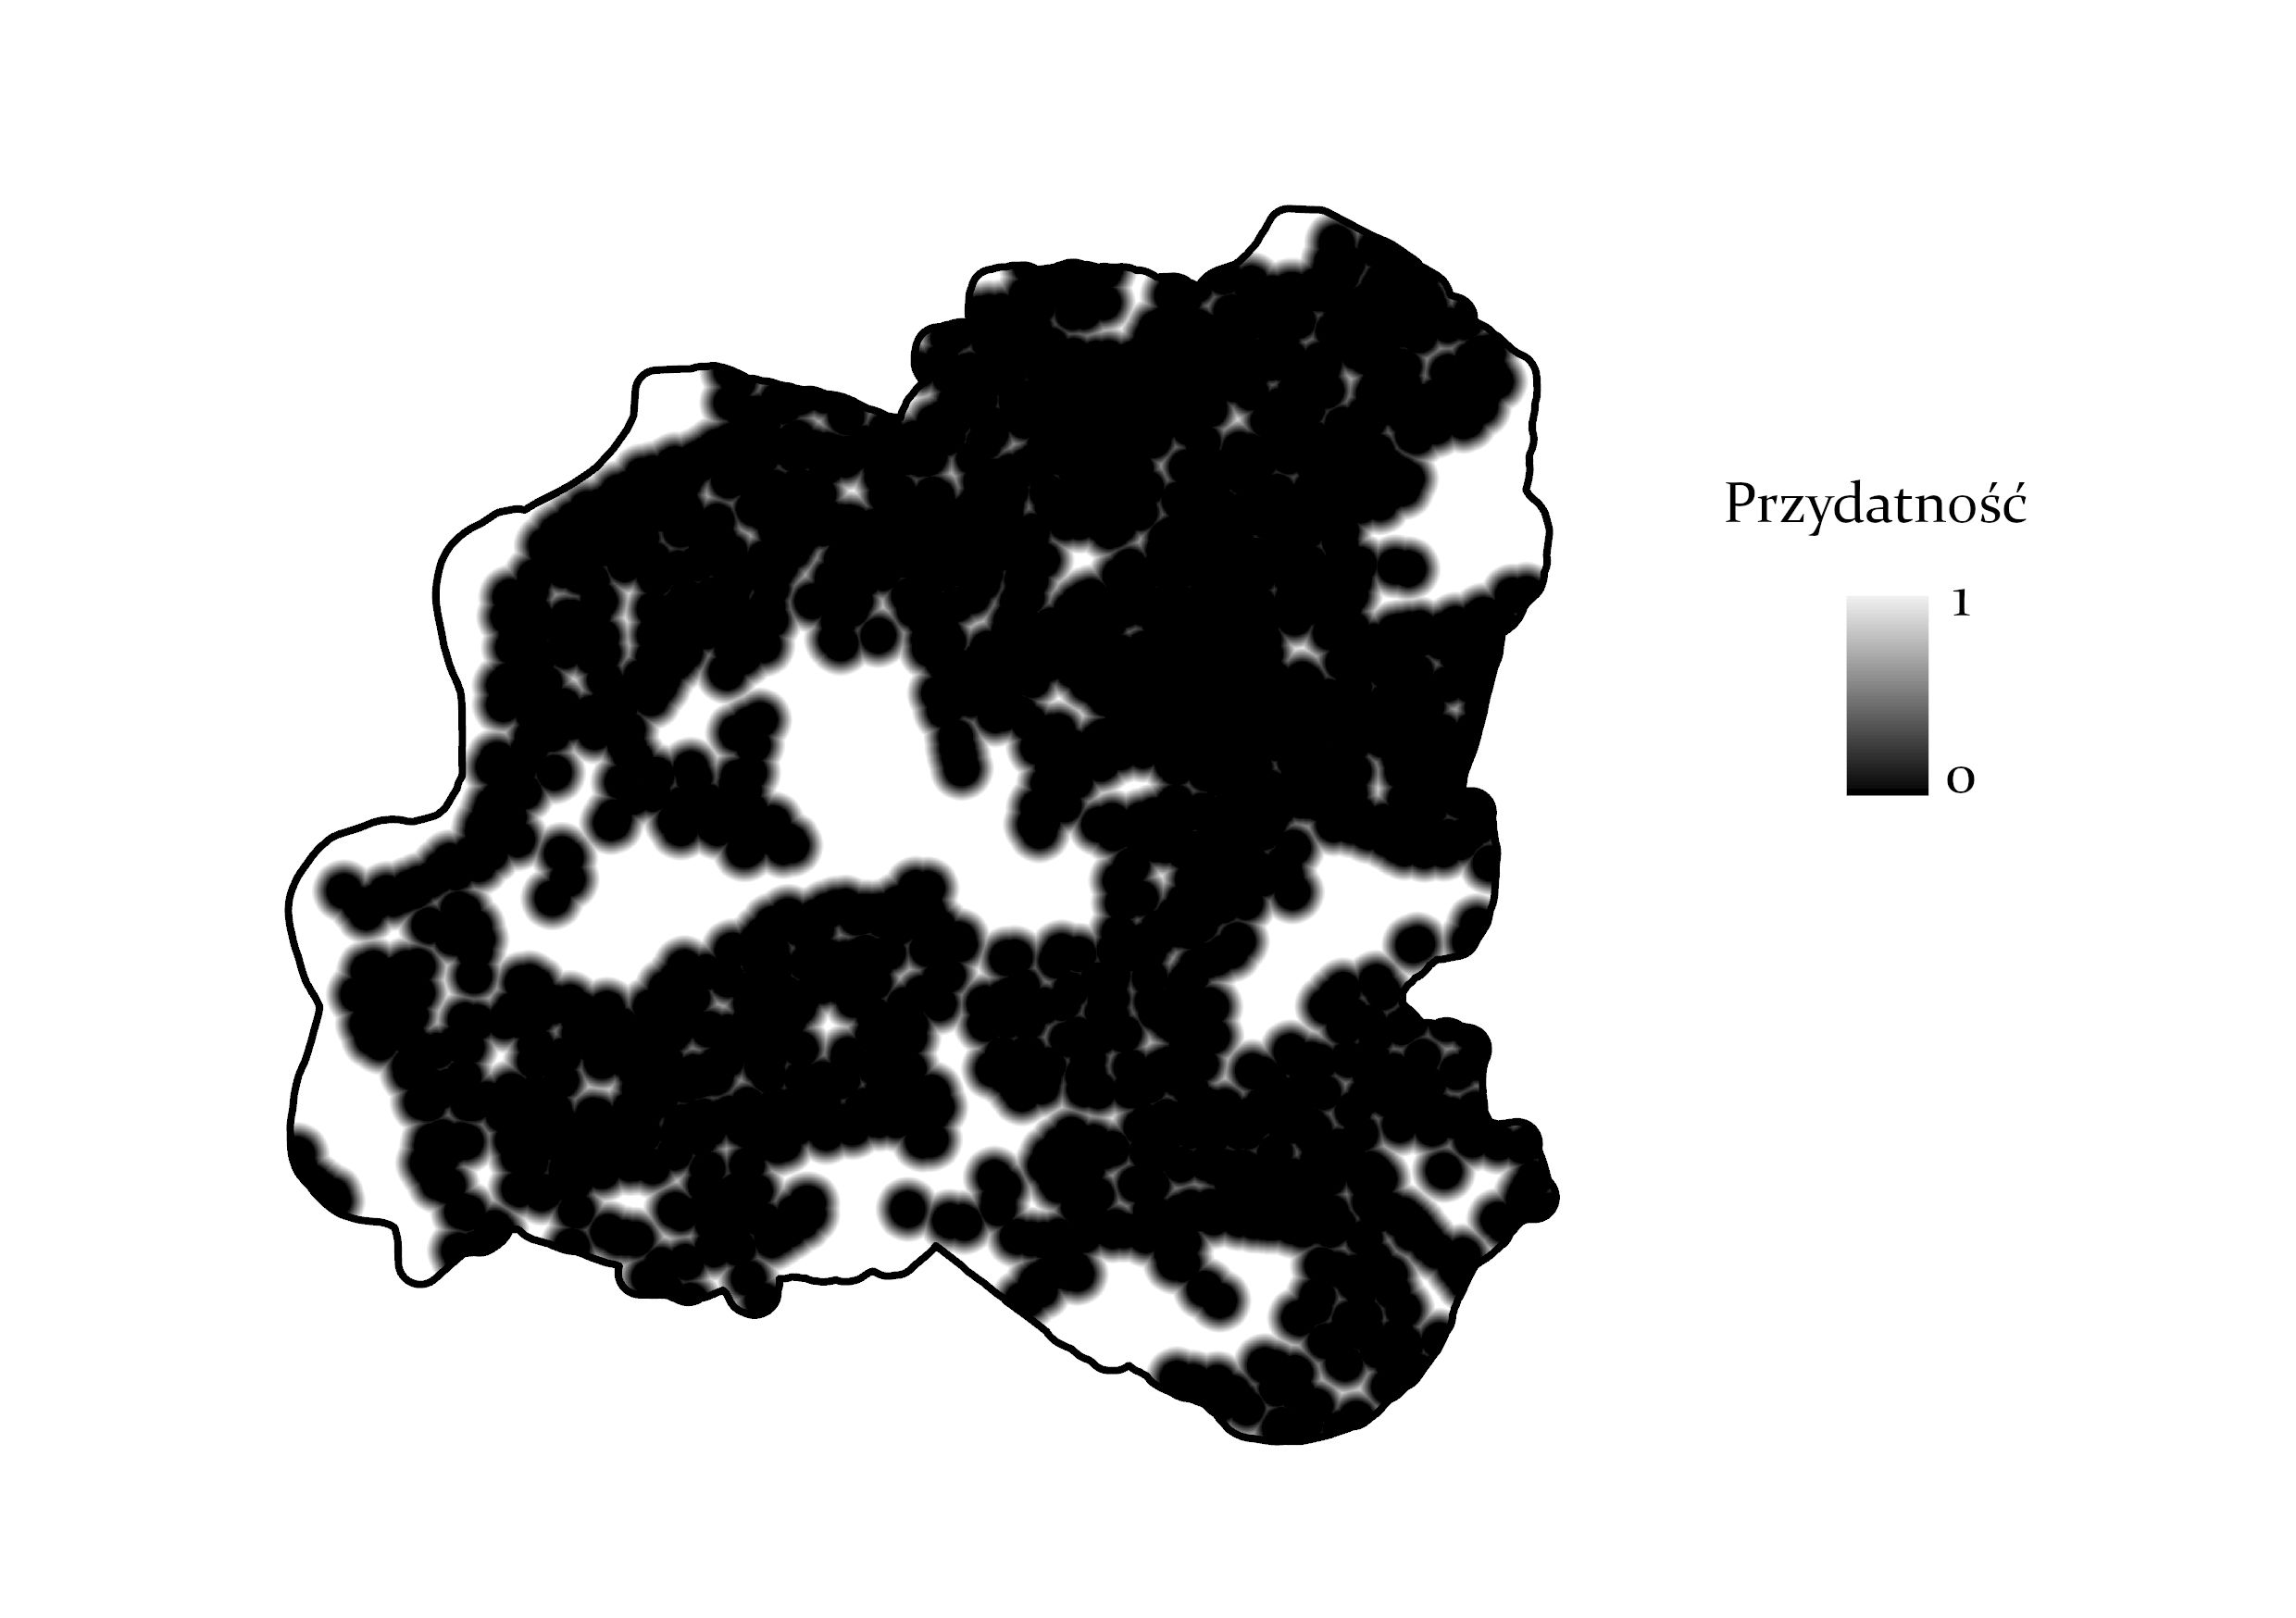
\includegraphics[width=0.75\textwidth]{img/plesna-kryterium2-layout.jpg}
    \caption{Mapa przydatności dla kryterium 2.}
\end{figure}

\begin{figure}[H]
    \centering
    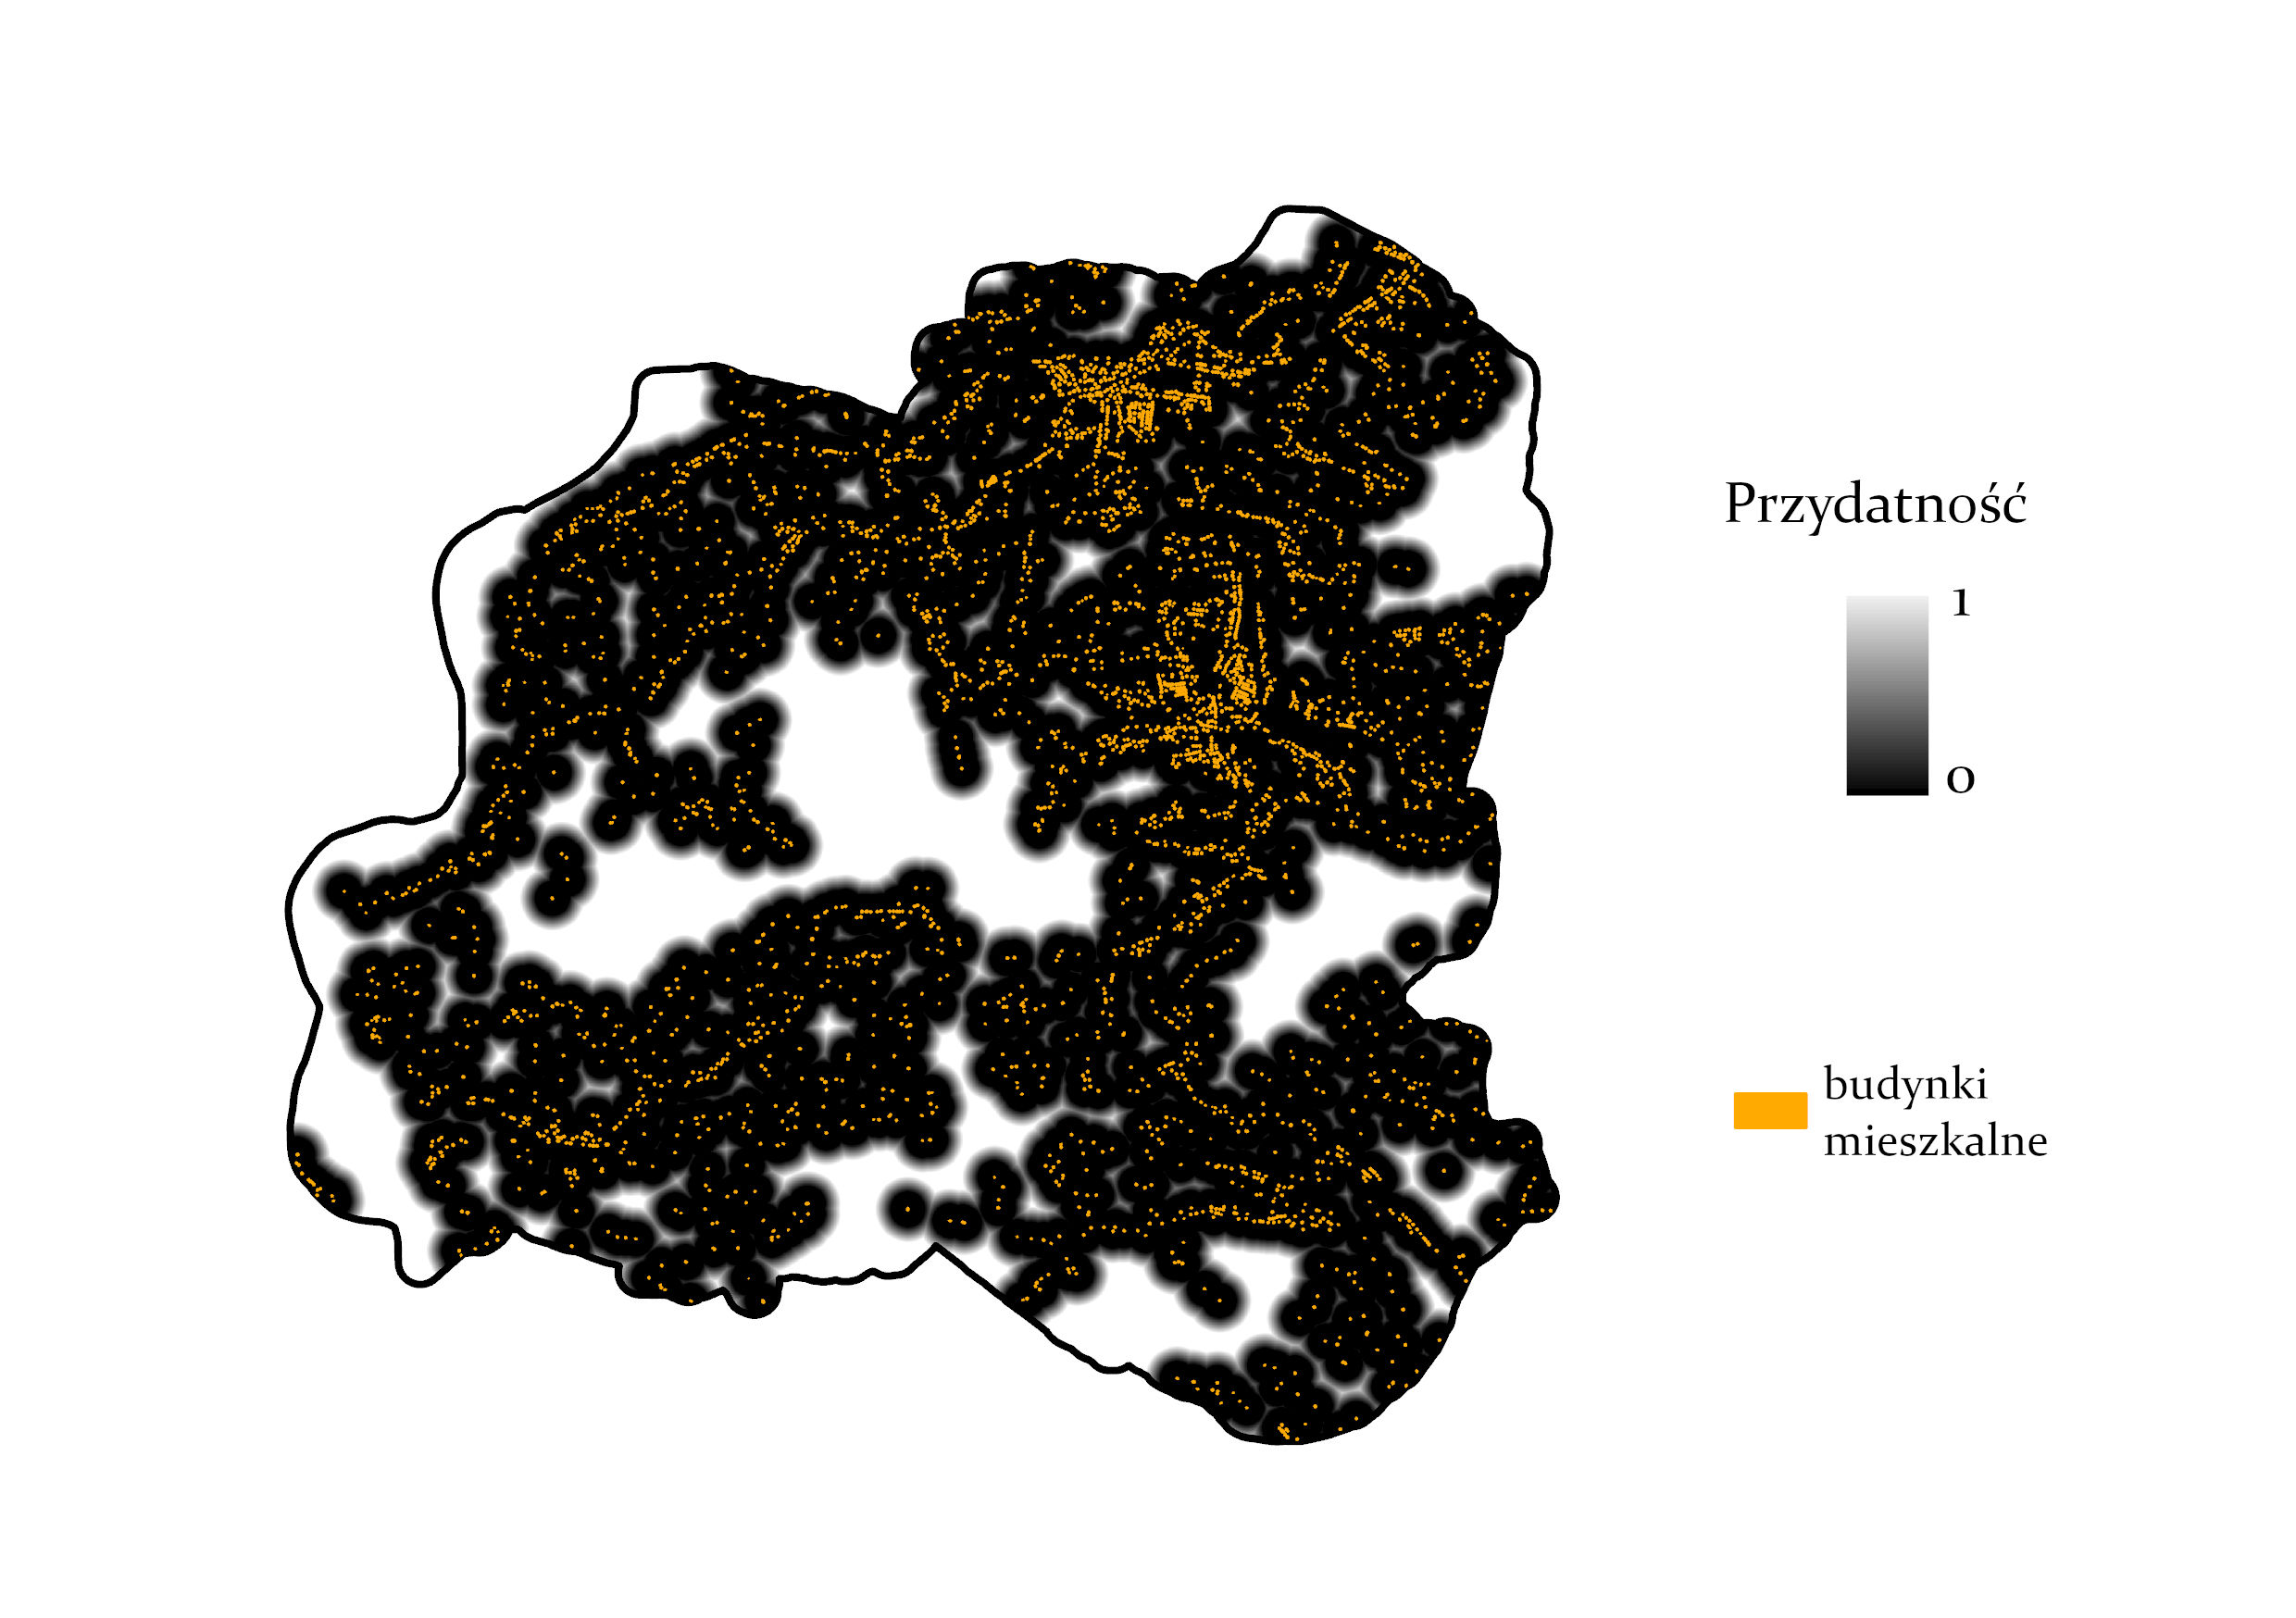
\includegraphics[width=0.75\textwidth]{img/plesna-kryterium2-budynki.jpg}
    \caption{Mapa przydatności dla kryterium 2. zawierająca budynki mieszkalne}
\end{figure}

\subsection{Kryterium 3: pokrycie terenu}
Duża część obszaru, która dla kryterium 2. przyjęła dużą przydatność, tutaj zostaje całkowicie wyeliminowana ze względu na pojawienie się tam terenów leśnych.

\begin{figure}[H]
    \centering
    \includegraphics[width=0.75\textwidth]{img/plesna-kryterium3-layout.jpg}
    \caption{Mapa przydatności dla kryterium 3.}
\end{figure}

\begin{figure}[H]
    \centering
    \includegraphics[width=0.75\textwidth]{img/plesna-kryterium3-lasy.jpg}
    \caption{Mapa przydatności dla kryterium 3. zawierająca lasy}
\end{figure}

\subsection{Kryterium 4: dostęp do dróg utwardzonych}
Stosunkowo duża część obszaru, w porównaniu do poprzednich kryteriów, cechuje się dużą przydatnością dla tego kryterium.

\begin{figure}[H]
    \centering
    \includegraphics[width=0.75\textwidth]{img/plesna-kryterium4-layout.jpg}
    \caption{Mapa przydatności dla kryterium 4.}
\end{figure}

\begin{figure}[H]
    \centering
    \includegraphics[width=0.75\textwidth]{img/plesna-kryterium4-drogi.jpg}
    \caption{Mapa przydatności dla kryterium 4. zawierająca drogi utwardzone}
\end{figure}

\subsection{Kryterium 5: nachylenie stoków}
Gmina ta również jest gminą o stosunkowo dużych nachyleniach stoków. Lecz istnieją również w niej tereny o niższych stokach, na zachodzie oraz północnym wschodzie.


\begin{figure}[H]
    \centering
    \includegraphics[width=0.75\textwidth]{img/plesna-kryterium5-layout.jpg}
    \caption{Mapa przydatności dla kryterium 5.}
\end{figure}

\begin{figure}[H]
    \centering
    \includegraphics[width=0.75\textwidth]{img/plesna-kryterium5-stoki.jpg}
    \caption{Mapa nachyleń stoków wykorzystana podczas sprawdzania kryterium 5.}
\end{figure}


\subsection{Kryterium 6: dostęp do światła słonecznego}
Pod względem tego kryterium gmina wydaje się w dużej części korzystnie uwarunkowana.

\begin{figure}[H]
    \centering
    \includegraphics[width=0.75\textwidth]{img/plesna-kryterium6-layout.jpg}
    \caption{Mapa przydatności dla kryterium 6.}
\end{figure}

\begin{figure}[H]
    \centering
    \includegraphics[width=0.75\textwidth]{img/plesna-kryterium6-aspect.jpg}
    \caption{Mapa przydatności dla kryterium 6. zawierająca stopień wystawy słonecznej}
\end{figure}

\subsection{Kryterium 7: dojazd do istotnych drogowych węzłów komunikacyjnych}

\begin{figure}[H]
    \centering
    \includegraphics[width=0.75\textwidth]{img/plesna-kryterium7-layout.jpg}
    \caption{Mapa przydatności dla kryterium 7.}
\end{figure}

\begin{figure}[H]
    \centering
    \includegraphics[width=0.75\textwidth]{img/plesna-kryterium7-wezly.jpg}
    \caption{Mapa odległości od węzłów}
\end{figure}

\subsection{Ocena przydatności terenu}
\begin{figure}[H]
    \centering
    \includegraphics[width=0.75\textwidth]{img/plesna-rozmyte-layout.jpg}
    \caption{Suma kryteriów rozmytych}
\end{figure}

Ogromna część obszaru gminy jest zupełnie nieprzydatna do inwestycji ze względu na bliskość budynków mieszkalnych, lasów czy wody. Elementy te wzajemnie się uzupełniają i jeżeli na terenie nie ma budynków mieszkalnych, to istnieje tam las, albo przepływa tam rzeka. W wyniku tego niemal cała gmina jest czarną plamą oznaczającą zerową przydatność.

\begin{figure}[H]
    \centering
    \includegraphics[width=0.75\textwidth]{img/plesna-ostre-layout.jpg}
    \caption{Suma kryteriów ostrych}
\end{figure}

\begin{figure}[H]
    \centering
    \includegraphics[width=0.75\textwidth]{img/plesna-wynik.jpg}
    \caption{Wynik łączenia kryteriów ostrych i rozmytych}
\end{figure}

Niewielkie obszary przydatne, jakie pozostały po połączeniu kryteriów, znajdują się głównie w zachodniej części gminy Pleśna.

\begin{figure}[H]
    \centering
    \includegraphics[width=0.75\textwidth]{img/plesna-wynik-po-reklasyfikacji.jpg}
    \caption{Wynik łączenia kryteriów ostrych i rozmytych po reklasyfikacji}
\end{figure}

\subsection{Wybór przydatnych działek}

Pomimo nikłej obecności terenów przydatnych pod tę inwestycję w gminie, udało się wyłonić 4 grupy działek (z czego 2 z nich są przecięte jedynie drogą, więc możnaby je połączyć).

\begin{figure}[H]
    \centering
    \includegraphics[width=0.75\textwidth]{img/plesna-przydatne-dzialki.jpg}
    \caption{Mapa przedstawiająca przydatne działki}
\end{figure}

\begin{figure}[H]
    \centering
    \includegraphics[width=0.75\textwidth]{img/plesna-dzialki-przydatne-ortofoto.jpg}
    \caption{Mapa przedstawiająca przydatne działki na ortofotomapie}
\end{figure}

\begin{figure}[H]
    \centering
    \includegraphics[width=0.75\textwidth]{img/plesna-dzialki-przydatne-ortofoto-2.jpg}
    \caption{Mapa przedstawiająca przydatne działki na ortofotomapie}
\end{figure}

\subsection{Przyłącze do sieci SN}
\begin{figure}[H]
    \centering
    \includegraphics[width=0.75\textwidth]{img/plesna-cost-raster.jpg}
    \caption{Mapa kosztów względnych}
\end{figure}

\begin{figure}[H]
    \centering
    \includegraphics[width=0.75\textwidth]{img/plesna-cost-backlink.jpg}
    \caption{Mapa kierunków (backlink)}
\end{figure}

\begin{figure}[H]
    \centering
    \includegraphics[width=0.75\textwidth]{img/plesna-cost-distance.jpg}
    \caption{Mapa kosztów skumulowanych}
\end{figure}

\begin{figure}[H]
    \centering
    \includegraphics[width=0.75\textwidth]{img/plesna-dzialki-linie.jpg}
    \caption{Mapa przedstawiająca przydatne działki oraz linie elektroenergetyczne}
\end{figure}

Przez jedną z wytypowanych grup działek przechodzi już linia elektroenergetyczna, w związku z czym ścieżka przyłącza nie została utworzona.

\begin{figure}[H]
    \centering
    \includegraphics[width=0.75\textwidth]{img/plesna-braksciezki.jpg}
    \caption{Mapa przedstawiająca linie elektroenergetyczne przechodzące przez jedną z grup działek}
\end{figure}


\end{document}